% thesis.tex
%
% Copyright 2022 Alexander Lyttle.
%
% This work may be distributed and/or modified under the conditions of the
% LaTeX Project Public License (LPPL) version 1.3 or later.
%
% The latest version of this license is in
% https://www.latex-project.org/lppl.txt and version 1.3 or later is part of
% all distributions of LaTeX version 2005/12/01 or later.
%
%
%% PREAMBLE ===================================================================
%
% UoB recommends A4 paper and a font size of 12pt
\documentclass[a4paper,12pt]{uobthesis}


%% PACKAGES -------------------------------------------------------------------
%
% Packages and setup are in packages.sty
% Use 'print' option for print version (reduced color)
% Use 'editor' option for line numbers
\usepackage[editor]{packages}
% AAS macro package
\usepackage{aas_macros}

% Add any additional packages below or at the bottom of packages.sty


%% RESOURCES ------------------------------------------------------------------
%
% Add bibliography resource files
\addbibresource{references.bib}
\addbibresource{lyttle21.bib}

% Add glossary files
% glossary/acronyms.tex
%
% Copyright 2022 Alexander Lyttle.
%
% This work may be distributed and/or modified under the conditions of the
% LaTeX Project Public License (LPPL) version 1.3 or later.
%
% The latest version of this license is in
% https://www.latex-project.org/lppl.txt and version 1.3 or later is part of
% all distributions of LaTeX version 2005/12/01 or later.
%
%
%% GLOSSARY OF ACRONYMS =======================================================
%
% For the list of acronyms to appear, you need to:
% pdflatex thesis.tex
% makeglossaries thesis
% pdflatex thesis.tex
%
% List your acronyms here, e.g.
\newacronym{ms}{MS}{main sequence}
\newacronym{dpi}{DPI}{dots per inch}

% glossary/terms.tex
%
% Copyright 2022 Alexander Lyttle.
%
% This work may be distributed and/or modified under the conditions of the
% LaTeX Project Public License (LPPL) version 1.3 or later.
%
% The latest version of this license is in
% https://www.latex-project.org/lppl.txt and version 1.3 or later is part of
% all distributions of LaTeX version 2005/12/01 or later.
%
%
%% GLOSSARY OF TERMS ==========================================================
%
% For the list of terms to appear, you need to:
% pdflatex thesis.tex
% makeglossaries thesis
% pdflatex thesis.tex
%
% List of terms go here, e.g.
\newglossaryentry{luminosity}
{
    name=luminosity,
    description={The total radiant power of an object}
}
\newglossaryentry{star}
{
    name=star,
    description={An astronomical object which is in hydrostatic equilibrium and emits light due to internal sources of energy}
}


% Specify which files to include (for faster compile time)
\includeonly{
  chapters/introduction,
  chapters/hbm,
  chapters/lyttle21,
  chapters/glitch,
  chapters/glitch-gp,
  chapters/conclusion,
  appendices/lyttle21
}

%% TITLEPAGE DETAILS ----------------------------------------------------------
%
% Add your details here
\author{Alexander J. Lyttle}
\title{Hierarchically Modelling Many Stars}
\group{Sun, Stars and Exoplanets Group}
\school{Physics and Astronomy}
\college{Engineering and Physical Sciences}
\submitted{April}{2023}  % Change this to the month you submit your thesis

% Path to UoB logo file, downloaded from 
% https://intranet.birmingham.ac.uk/staff/resources/brand-resources/university-logo-guidelines.aspx
\logo{uob-logo.eps}  % Optional, comment this out if logo not wanted


%% LICENSE --------------------------------------------------------------------
%
% Optional license, uncomment this if you want to use custom license text
% Default text is 'All Rights Reserved.'
\license{\doclicenseText}  % This example uses the doclicense package


%% DEDICATION -----------------------------------------------------------------
%
% Optional dedication, edit this or comment out if not appropriate
\dedication{%
\begin{center}
  \textsc{Dedicated to}\\
  Hannah\\
  \pgfornament[width=1.5cm,ydelta=-3pt]{70}\\  % Fancy divider
  % \pgfornament[width=2.5cm,ydelta=-3pt]{80}\\  % Simple divider
  \textsc{In Loving Memory of}\\
  Angela and Barry
\end{center}
}


%% ABSTRACT -------------------------------------------------------------------
%
\abstract{%
As high-precision asteroseismology modelling of stars continues to advance, it is becoming increasingly important to account for the systematic effects that arise from our assumptions of the stellar helium abundance (\(Y\)) and the mixing-length theory parameter (\(\mlt\)). To address this issue, we present a novel approach for improving the inference of the fundamental parameters of a sample of Kepler dwarfs and subgiants with a narrow mass range of \(0.8 < M < 1.2 \mathrm{M}_{\odot}\). Our method includes a statistical treatment of \(Y\) and \(\mlt\) and employs a hierarchical Bayesian model that incorporates information about the distribution of these parameters in the population. Specifically, we fit a linear helium enrichment law that includes an intrinsic scatter and a normal distribution in \(\mlt\). We explore various levels of pooling parameters, with and without the Sun as a calibrator, and report \(\Delta Y/\Delta Z = 1.05^{+0.28}_{-0.25}\) and \(\mu_\alpha = 1.90^{+0.10}_{-0.09}\) when the Sun is included. Despite accounting for the uncertainties in \(Y\) and \(\mlt\), we are able to report statistical uncertainties of 2.5 per cent in mass, 1.2 per cent in radius, and 12 per cent in age. Moreover, our approach can be extended to larger samples, which would enable us to obtain more precise constraints on the fundamental parameters of individual stars and improve our understanding of the population-level inference.
}


%% ACKNOWLEDGEMENTS -----------------------------------------------------------
%
\acknowledgements{%
\begin{CJK*}{UTF8}{gbsn}
  % INTERNAL SUPPORT
  I am tremendously grateful to my PhD supervisor Guy R. Davies for his support and excellent mentorship throughout my postgraduate research. I also thank my first co-supervisor Andrea Miglio for his guidence before his move to the University of Bologna. I extend my thanks to Amaury Triaud, who took over from Andrea as my co-supervisor and has since been an inspiring mentor and leader of our research group. It has been a pleasure to work with the Sun, Stars, and Exoplanets research group here at the University of Birmignham. Particularly, I would like to thank all of my fellow current and former PhD students with whom I have exchanged ideas, advice, laughs, and stories: T. Baycroft, L. Carboneau, Y. Davies, A. Dixon, G. Dransfield, A. Freckleton, O. Hall, E. Hatt, V. Hod\v{z}i\'{c}, S. Khan, E. Ross, O. Scutt, M. Standing, W. Van Rossem, and E. Willett. I also appreciate the support of other postdoctoral researchers in our group, notably M. Nielsen, Tanda Li (李坦达), and W. Ball. I extend my thanks to the support staff in the School of Physics and Astronomy, particularly our office secretary Lou for her unwavering support over a challenging few years.
\end{CJK*}

% EXTERNAL COLLABORATORS
I thank my external collaborators. Nick Saunders at the University of Hawaii. Simon Murphy at the University of Southern Queensland. Co-authors on my research publications.

% FUNDING
I acknowledge the support of the public who have indirectly funded the research in this work via various public agencies. Particularly, I thank the Science and Technology Facilities Council who funded my PhD. I also acknowledge that this work is a part of a project that has received funding from the European Research Council (ERC) under the European Union's Horizon 2020 research and innovation programme (CartographY; grant agreement ID 804752). Finally, I am grateful for the financial and academic support from the Alan Turing Enrichment scheme. This scheme provided me the opportunity to learn from and collaborate with the wider world of machine learning in science.

% DATA AND SOFTWARE
The use of data and software. Open source community. This work made use of the \href{https://gaia-kepler.fun}{gaia-kepler.fun} crossmatch database created by Megan Bedell.

% FAMILY AND FRIENDS
Support of my loving family and friends.

% THESIS EXAMINERS
Finally, I would like to thank my PhD examiners Daniel Reese and Chris Moore, and viva chairperson Annelies Mortier.
}


%% DOCUMENT ===================================================================
%
\begin{document}

  \maketitle  % Title page

  \frontmatter

  %% FRONT MATTER -------------------------------------------------------------
  \makefrontmatter  % Adds abstract, dedication and acknowledgements

  %% CONTENTS -----------------------------------------------------------------
  \tableofcontents
  \listoffigures                                              % Figures
  \listoftables                                               % Tables
  \printglossary[type=\acronymtype,title={List of Acronyms}]  % Acronyms
  \printglossary[title={List of Terms}]                       % Terms

  \mainmatter

  %% CHAPTERS -----------------------------------------------------------------
  %
  % Add your chapters here
  % chapters/introduction.tex
%
% Copyright 2022 Alexander Lyttle.
%
% This work may be distributed and/or modified under the conditions of the
% LaTeX Project Public License (LPPL) version 1.3 or later.
%
% The latest version of this license is in
% https://www.latex-project.org/lppl.txt and version 1.3 or later is part of
% all distributions of LaTeX version 2005/12/01 or later.
%
%
\chapter[Introduction]{Introduction}

\textit{In this chapter, I introduce the current state of modelling stars with asteroseismology and the types of stars being studied in this thesis. I start with a brief history of understanding the stars spanning the last century. In Section \ref{sec:seismo}, I introduce asteroseismology of stars which oscillate like the Sun. Then, I provide examples of asteroseismology being used to model large samples of dwarf and subgiant stars in Section \ref{sec:many-stars}. Finally, I introduce the concept of modelling stars the `Bayesian way' with some examples of current methods and their limitations.}

% Since the late 19th century, astronomers have been trying to understand the physical structure and evolution of the Sun and other stars. They wanted to determine whether other stars were like the Sun and whether they changed with time. Answers to these questions could tell us where we came from and what the future holds for the solar system. While little was known of this at the time, astronomers started by gathering data in an effort to map the night sky. The invention of the spectrograph by \citet{Draper1874} allowed researchers to systematically classify stars by their brightness in different wavelengths of light \citep{Maury.Pickering1897}. This was an pivotal early step towards the large-scale stellar surveys we are used to today.

% \citet{Hertzsprung1909} made early estimates of absolute magnitude from the widths of the spectral lines

\section{Understanding the Stars}\label{sec:stars}

Early efforts to understand the stars began by finding relations between their spectral classification and magnitude in different photometric bands. On what was later called a Hertzsprung-Russell (HR) diagram \citep[e.g.][]{Russell1914}, astronomers plot the absolute magnitude (or luminosity, \(L\)) of a star against its spectral class (or effective temperature, \(\teff\)). They found that stars were not uniformly distributed on the HR diagram, but were instead grouped in distinct sequences. For example, the narrow diagonal band where most stars were found was called the \emph{main sequence}. Astronomers wondered why stars adhered to these sequences and to what extent they evolved with time.

Initial insight into stellar evolution came about when astronomers studied open clusters on the HR diagram \citep{Trumpler1930}. These are groups of stars found at a similar distance and close together on the sky. Assuming clusters formed at the same time with similar chemical abundances, the only expected difference between stars is their mass and multiplicity. Using stars of known mass (e.g. from orbital solutions to binary systems) and luminosity distributions, astronomers could trace lines of similar mass and composition from younger to older clusters \citep[e.g.][]{Sandage1957}. Coupled with early arguments from stellar physics \citep[e.g.][]{Chandrasekhar1939}, scientists formed stellar evolutionary tracks --- the path a star takes on the HR diagram during its evolution. Deriving the stellar radius (\(R\)) from the relation \(L \propto R^2 \teff^4\), they inferred that stars started life on the dimmer edge of the main sequence and became brighter and larger throughout most of their lifetime. At some point, stars would leave the main sequence, rapidly cool, expand, and then ascend a region of the HR diagram known as the \emph{red giant branch}.

%  \citet{Kuiper1938} found an empirical mass-luminosity relation.

% Explaining structure in the HR diagram involved studying open clusters of stars. Astronomers expected these groups of stars, found at a similar parallax, to have formed at a similar time with similar chemical abundances. They presumed the remaining variation was for stars of different mass. Therefore, ordering open clusters on an HR diagram showed the evolution of stars of different mass. Furthermore, early measurements of stellar mass came from orbital solutions to visual and spectroscopic binary star systems.

% Observations of stars in clusters, assumed to have similar ages and chemical abundances, showed how stars of different mass evolved across the HR diagram with time.

% The luminosity and effective temperature could be estimated from the magnitude and colour of the stars. From luminosity and temperature, we could derive the radius of stars. Early stellar mass estimates came from visual and spectroscopic binaries. Spectroscopy provides abundances of chemical species ionised in the stellar atmosphere. However, except for the Sun, stellar age and helium abundance has no model-independence. The latter ionisations at temperatures and densities higher than the surface of stars like the Sun.

The chemical composition, energy sources and evolutionary physics of stars were still uncertain. Spectroscopy revealed relative abundances of elements excited in stellar atmospheres, but it was difficult to determine their absolute abundances. \citet{Payne1925} proposed that stars comprised mostly hydrogen and helium, later reinforced by estimates of helium content in the Sun \citep[e.g.][]{Schwarzschild1946}. The idea was radical at the time because it did not match the abundance of elements found on Earth. Meanwhile, advancements in nuclear science spawned the theory of stellar nucleosynthesis \citep{Hoyle1946}. Stars produce elements heavier than hydrogen and helium through nuclear fusion reactions. This discovery explained the production of many elements in the universe, tying the formation and evolution of stars to planetary formation and the conditions for life in the universe.

In the second half of the 20th century, astronomers advanced the theory of stellar evolution. With this came computational methods for simulating stars \citep[e.g.][]{Kippenhahn.Weigert.ea1967}. Astronomers could start to compare observations of stars and clusters with numerical solutions to stellar structure equations. We call this process \emph{modelling stars}. Early models of the Sun benefited from independent geological age estimates and neutrino-production rates from observing cosmic rays. With these constraints, and the Sun as a calibrator, researchers could start to refine their models and test them on other stars. For example, \citet{Iben1967} computed stellar models for main sequence stars with similar masses to the Sun using observations of the clusters M67 and NGC 188.

On a similar timescale, a new field emerged which gave astronomers a model-independent way of studying the inside of stars. Identifying regular perturbations of the surface of the Sun, researchers realised that they pertained to high-order, stochastically-driven spherical harmonic oscillations. Measuring these oscillation modes, they could study the Sun similarly to how seismologists study the Earth. Astronomers studying multiple non-radial stellar oscillations distinguished this new field, called \emph{asteroseismology}, from the well-known study of radially pulsating stars \citep[e.g. Cepheid variables;][]{Leavitt1908}. In Section \ref{sec:seismo} we briefly elaborate on the history and theory of asteroseismology for stars like the Sun.

% Approximations for the equation of state by \citet{Eggleton.Faulkner.ea1973}.

Today, astronomers have a huge abundance of data with which to determine stellar parameters and test theories of stellar evolution. In Section \ref{sec:many-stars}, we give some recent examples of Sun-like asteroseismic populations and their context in the wider HR diagram. With big datasets and complex, multi-parameter models, there has been a recent shift towards Bayesian statistical methods to model these stars. THerefore, we introduce the concept of modelling stars `the Bayesian way' in Section \ref{sec:modelling-stars}. There, we introduce some tools used to model these stars and then highlight some common assumptions made.

% Large-scale surveys have lead to asteroseismology on a large scale. Combined with photometry, spectroscopy and astrometry (parallax, position and motion), asteroseismology has bePowerful tool in Section \ref{sec:many-stars}.

% Modelling stars became a way to test theories of stellar evolution and estimate the ages of stars. In recent years, the Bayesian framework...  

% We briefly introduce modelling stars the Bayesian way in Section \ref{sec:modelling-stars}.

% On a similar timescale, the field of helioseismology emerged. Starting by observing oscillations on the surface of the Sun. When applied to other stars, asteroseismology. This gave highly precise measurements of the oscillation modes. Solar-like oscillators oscillate like the Sun. These provided an independent way to test stellar models and determine masses and radii from the scaling relations.

\section[Solar-Like Oscillators]{Asteroseismology of Solar-Like Oscillators}\label{sec:seismo}

% In this section, we provide a brief history and theory of asteroseismology to provide a foundation from which to understand this thesis. However, we recommend the recent review by \citet{Aerts2021} or the lecture notes by \citet{Christensen-Dalsgaard2014} for a more detailed understanding of the field.

\subsection{A Brief History of Asteroseismology}

Several decades ago, 5-minute oscillations in the radial velocity of the solar surface were observed by \citet{Leighton.Noyes.ea1962}, leading to the inference of acoustic waves trapped beneath the solar photosphere \citep{Ulrich1970}. A further decade of study culminated in the measurement of regular patterns of oscillation modes in the Sun; for example, from measurements of radial velocity \citep{Claverie.Isaak.ea1979} and total irradiance \citep{Woodard.Hudson1983a}. Initially thought to be short-lived irregularities on the surface, these modes were found to be compatible with stochastically excited standing waves penetrating deep into the Sun. Later, \citet{Deubner.Gough1984} introduced the word \emph{helioseismology} to describe the study of the solar interior using observations of these modes. Helioseismology was soon responsible for breakthrough solar research, from measuring differential rotation \citep{Deubner.Ulrich.ea1979} to solving the mismatch between predicted and measured solar neutrino production \citep{Bahcall.Ulrich1988}.

Astronomers initially debated the mechanism driving the modes of standing pressure waves (or \emph{p modes}) in the Sun. \citet{Goldreich.Keeley1977} suggested what became the prevailing theory, that the p modes were stochastically excited by near-surface convection. Therefore, astronomers expected solar-like oscillations to be present in other stars with a convective envelope like the Sun. Shortly thereafter, \citet{Christensen-Dalsgaard1984} was among those to introduce the term \emph{asteroseismology} --- the study of the internal structure of stars with many observable oscillation modes. Subsequently, solar-like oscillations were discovered in a few bright stars. Among the first were Procyon and \(\alpha\) Cen A \citep{Gelly.Grec.ea1986}, with individual modes later resolved by \citet{Martic.Schmitt.ea1999} and \citet{Bouchy.Carrier2001} respectively.

Instrumental and atmospheric noise limited the progress of asteroseismology with ground-based equipment to studies of small number of bright dwarf stars. Asteroseismology of solar-like oscillators requires high-cadence (\(\sim \SIrange{1}{10}{\minute}\)) brightness observations over long baselines (\(\sim \SI{1}{\year}\)) with parts-per-million precision \citep[e.g.][]{Schofield.Chaplin.ea2019}. 
% For example, noise of \(\lesssim \SI{100}{ppm\per\hour}\) for \(I\)-band magnitudes \(\lesssim 10\) \citep{Schofield.Chaplin.ea2019}. 
The first dedicated space-based missions which met these requirements arrived in the late 2000s, accelerating progress in the field. Initially, the \emph{CoRoT} mission \citep{Baglin.Auvergne.ea2006} detected solar-like oscillations in thousands of red giant stars \citep{DeRidder.Barban.ea2009,Mosser.Belkacem.ea2010}. Then, the \emph{Kepler} mission \citep{Borucki.Koch.ea2010} yielded oscillations in thousands more red giants \citep{Pinsonneault.Elsworth.ea2014} and hundreds of main sequence stars similar to the Sun \citep{Serenelli.Johnson.ea2017}. Most recently, \emph{TESS} \citep{Ricker.Winn.ea2015} added thousands more dwarf and giant stars to the roster of solar-like oscillators \citep{Hon.Huber.ea2021,SilvaAguirre.Stello.ea2020,Hatt.Nielsen.ea2023}. For a more detailed review of modern asteroseismology, see \citet{Aerts2021}. 

\subsection{A Brief Theory of Solar-Like Oscillations}\label{sec:seismo-theory}

\begin{figure}[tb]
    \centering
    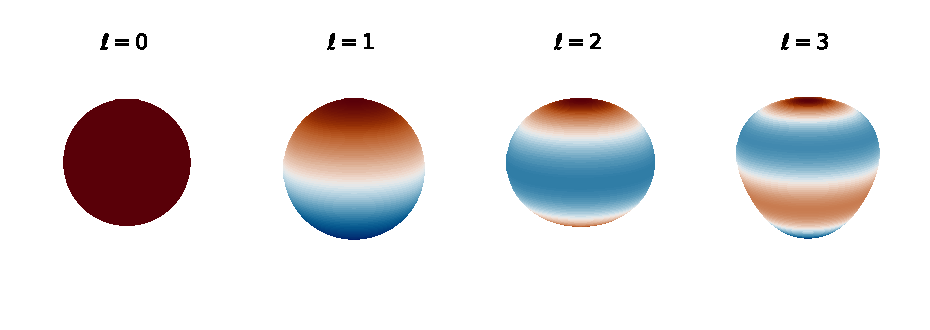
\includegraphics[trim={0 0.4in 0 0},clip]{figures/spherical_harmonics.pdf}
    \caption[Surface spherical harmonic oscillation modes for a few angular degrees ($l$) with azimuthal order \(m=0\).]{Surface spherical harmonic oscillation modes for a few angular degrees ($l$) with azimuthal order \(m=0\). The colour-map represents radial displacement at the surface, with \emph{red} and \emph{blue} corresponding to displacement inward and outward respectively. The coloured regions pulsate in and out, and the white regions represent stationary nodes on the surface.}
    \label{fig:spherical-harmonics}
\end{figure}

We can approximate oscillations on the surface of a star by spherical harmonic functions with angular degree \(l\) and azimuthal order \(m\). The angular degree is the number of nodes on the surface of the star. We show a representation of the surface spherical harmonics for the first four angular degrees in Figure \ref{fig:spherical-harmonics}. For each \(l\), there exists \(2l+1\) solutions with different azimuthal order (\(m\)) corresponding to the different orientations of the nodes over the spherical surface. Additionally, the oscillation modes have unique frequency solutions for different radial orders (\(n\)) proportional to the number of nodes radially throughout the star.

\begin{figure}[tb]
    \centering
    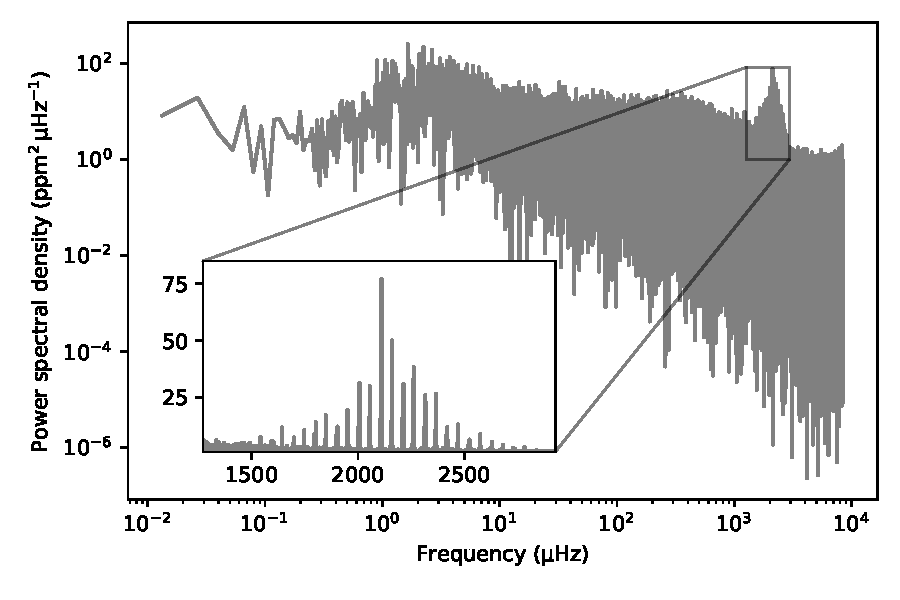
\includegraphics{figures/seismo-psd.pdf}
    \caption[The power spectral density of 16 Cyg A.]{The power spectral density of 16 Cyg A. The inset plot highlights the Gaussian-like power excess in the larger plot.}
    \label{fig:seismo-psd}
\end{figure}

In solar-like oscillators, p modes are stochastically excited by near-surface convection. Typically, the timescale of this process drives high-order modes in main sequence stars (\(n \sim 20\)). We can identify these modes in a frequency-power spectrum derived from photometric or radial velocity time series observations. For instance, both stars in the 16 Cygni planet hosting system are solar-like oscillators with similar properties to the Sun \citep{Metcalfe.Chaplin.ea2012,Davies.Chaplin.ea2015,Metcalfe.Creevey.ea2014}. Using 16 Cyg A as an example, we downloaded the power spectrum determined by the \emph{Kepler} Asteroseismic Science Operations Centre (KASOC) using \emph{Kepler} observations\footnote{\url{https://kasoc.phys.au.dk}}. Shown in Figure \ref{fig:seismo-psd}, the power spectrum of 16 Cyg A has a distinct power excess around \SI{2000}{\micro\hertz}. 

The power excess has a Gaussian-like shape around frequencies compatible with the near-surface convective timescale responsible for mode excitation. We call the centre of this Gaussian the \emph{frequency at maximum power} (\(\numax\)). Dependent on near-surface conditions, \citet{Brown.Gilliland.ea1991} suggested \(\numax\) scales with the acoustic cut-off frequency --- the highest frequency at which acoustic waves can reflect near the stellar surface. Subsequently, \citet{Kjeldsen.Bedding1995} found that \(\numax \propto g\teff^{\,-1/2}\) where \(g\) and \(\teff\) are the near-surface gravitational field strength and effective temperature. Hence, \(\numax\) for a solar-like oscillator decreases as it evolves, from \(\sim \SI{1000}{\micro\hertz}\) on the main sequence to \(\sim \SI{10}{\micro\hertz}\) near the tip of the red giant branch.

Looking closely at the power excess in Figure \ref{fig:seismo-psd}, we can see a comb of approximately equally spaced peaks. Each peak corresponds to an oscillation mode, with their collective central frequencies and separations providing information about the internal stellar structure. Naturally, higher frequency modes correspond to higher radial order, \(n\). However, the angular degree and azimuthal order are harder to identify. We saw in Figure \ref{fig:spherical-harmonics} how modes of higher \(l\) have more anti-nodes on the surface. Therefore, the overall effect of the oscillations cancel out when measuring irradiance integrated over the stellar surface. Consequentially, observed mode amplitude decreases with \(l\), leaving only \(l \lesssim 3\) detectable. 
% Not Section 2.1 of JCD Lecture Notes (2014) derives this
Therefore, we can assume the tallest peaks are \(l=0,1\), and the smaller peaks are \(l=2,3\), all modulated by the wider Gaussian-like envelope.

Modes with different \(m\) cannot be distinguished for a spherically symmetric, non-rotating star. In the case of a rotating or distorted (asymmetric) star, the observed mode frequencies will split for different \(m\) via the Doppler effect. Measuring this splitting can constrain the rotation rate of the star \citep[e.g.][]{Davies.Chaplin.ea2015,Garcia.Ceillier.ea2014,Deheuvels.Garcia.ea2012}. Such studies have lead to breakthrough research on the rotational evolution of stars \citep[e.g.][]{Angus.Aigrain.ea2015,Hall.Davies.ea2021,vanSaders.Ceillier.ea2016}. However, we will hereafter consider only the case of a slowly rotating, spherically symmetric star.

For an acoustic wave in a one-dimensional homogeneous medium, we would expect each mode of oscillation to be an integer multiple of the fundamental mode. While the case for a star is more complicated, we can also approximate the frequencies for different modes as a multiple of a characteristic frequency. \citet{Tassoul1980} found that the modes could be approximated by assuming the asymptotic limit, where \(l/n \rightarrow 0\). This lead to the following expression for the frequency of a mode for a given \(n\) and \(l\) \citep[cf.][]{Gough1986},
%
\begin{equation}
    \nu_{nl} \simeq \left(n + \frac{l}{2} + \varepsilon\right) \nu_0 + O(\nu_{nl}^{-1}), \label{eq:asy}
\end{equation}
%
where \(\varepsilon\) is some constant offset and \(O(\nu_{nl}^{-1})\) represents higher order terms. The characteristic frequency (\(\nu_0\)) is the inverse of the acoustic diameter,
%
\begin{equation}
    \nu_0 = \left(2 \int_{0}^{R} \frac{\dd r}{c(r)}\right)^{-1},
\end{equation}
%
where \(c(r)\) is the sound speed as a function of radius (\(r\)), and \(R\) is the radius of the star. Similarly to other variable stars, \citet{Ulrich1986} found that this characteristic frequency relates to mean stellar density by \(\nu_0 \propto \overline{\rho}^{\,1/2}\). While \(\nu_0\) is not directly detectable in solar-like oscillators, we can approximate it by taking the difference between consecutive modes of the same angular degree, \(\Delta\nu_{nl} = \nu_{nl} - \nu_{n-1\,l}\). Thus, estimates of a global (or average) \emph{large frequency separation}, \(\Delta\nu\), can also provide information about the density of a star. This leads to independent constraint on stellar mass and radius (e.g. from scaling relations to the Sun).

\begin{figure}[tb]
    \centering
    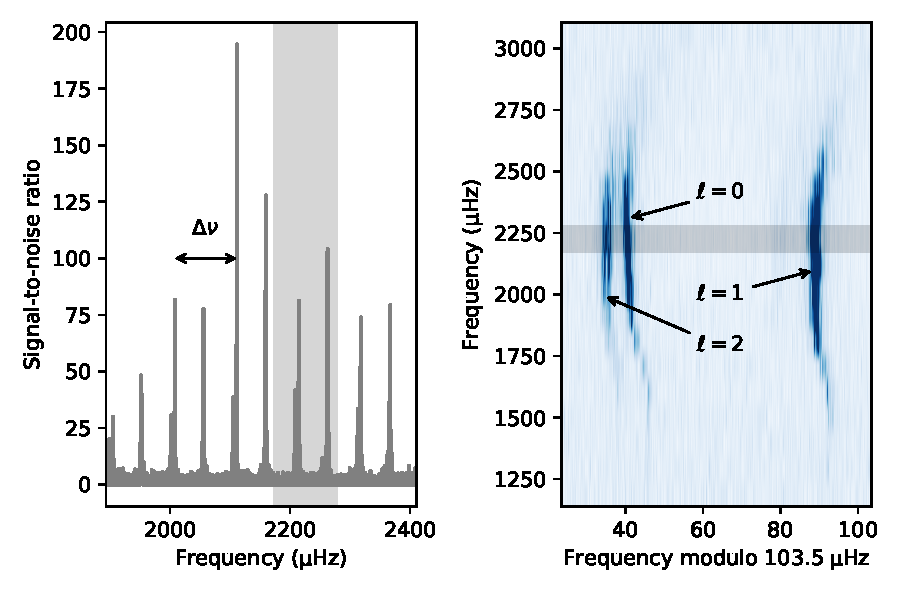
\includegraphics{figures/seismo-echelle.pdf}
    \caption[Signal-to-noise ratio as a function of frequency and echelle diagram for 16 Cyg A.]{\emph{Left:} A section of the spectral signal-to-noise ratio (SNR) against frequency for 16 Cyg A. The large frequency spacing (\(\Delta\nu\)) between two radial modes is annotated with a double-headed arrow. The shaded region corresponds to a single row (also highlighted) in the echelle plot (\emph{right}). The echelle plot shows the spectral SNR such that a darker colour represents a higher SNR. Each row spans \SI{103.5}{\micro\hertz} and is stacked in order of frequency. The apparent ridges are labelled according to the angular degree (\(l\)) of the modes they represent.}
    \label{fig:seismo-echelle}
\end{figure}

The asymptotic expression helps us identify modes in a star. If the first term of Equation \ref{eq:asy} was exact, we would expect odd and even modes to be grouped together and separated by \(\dnu/2\). To show this, we revisit the power spectrum of 16 Cyg A and estimate a signal-to-noise ratio (SNR) by dividing out a moving median in log-frequency steps of \SI{0.005}{\dex}. We can see the regular pattern predicted by Equation \ref{eq:asy} in the left panel of Figure \ref{fig:seismo-echelle}. Every other mode is approximately separated by \(\dnu\). To see this effect over the wider spectrum, we created an \emph{echelle} plot in the right panel. Folding the spectrum by an estimate of \(\dnu\) reveals a sequence of ridges corresponding to modes of different angular degree. Odd and even angular degree are grouped together, although do not lie on top of each other. The small difference between modes of different \(l\) is described by the higher order terms neglected from Equation \ref{eq:asy}. A faint ridge corresponding to \(l=3\) modes is also visible next to the \(l=1\) ridge. However, 16 Cyg A represents one of the highest SNR dwarf stars observed by \emph{Kepler}, and the \(l=3\) ridge is otherwise not usually visible. 

% Once we have identified a solar-like oscillator, what information is there to gain from asteroseismology? We have discussed how parameters \(\numax\) and \(\dnu\) scale with global stellar properties. Scaling these parameters with respect to the Sun, we can obtain relations for the radius and mass of the star,
% %
% \begin{align}
%     \left(\frac{R}{\si{\solarradius}}\right) &\simeq \left(\frac{\numax}{\numax_{,\odot}}\right) \left(\frac{\dnu}{\dnu_\odot}\right)^{-2} \left(\frac{\teff}{\teff_{,\odot}}\right)^{1/2},\\
%     \left(\frac{M}{\si{\soNonlarmass}}\right) &\simeq \left(\frac{\numax}{\numax_{,\odot}}\right)^3 \left(\frac{\dnu}{\dnu_\odot}\right)^{-4} \left(\frac{\teff}{\teff_{,\odot}}\right)^{3/2}.
% \end{align}
% %
% Using these relations directly can provide quick-look, independent mass and radius estimates \citep[e.g.][]{Pinsonneault.Elsworth.ea2018}.

% We can also use individual modes and compare with models. Worth noting the surface term here.

Repeating this kind of analysis on a large-scale can provide a wealth of observables from which to model stars. In the next section, we give some examples where asteroseismology was used to model many solar-like oscillators.

\section[Modelling Stars with Asteroseismology]{Modelling Many Stars with Asteroseismology}\label{sec:many-stars}

Recent space-based missions like \emph{Kepler} and \emph{TESS} enable asteroseismology with many stars. Like \emph{CoRoT}, these missions were primarily designed to detect exoplanets using the transit method. However, their instrumental requirements were also well-suited to asteroseismology. This allowed astronomers to study regions of the HR diagram in more detail, from main sequence dwarf stars to red giants. We draw particular attention to \emph{Kepler}, the first of the two missions. \emph{Kepler}'s primary mission observed a single \(\sim\SI{100}{deg\squared}\) diameter patch of sky for around 4 years \citep{Borucki.Koch.ea2010}, cut short by a mechanical failure which spawned the secondary \emph{K2} mission \citep{Howell.Sobeck.ea2014}. \emph{Kepler} took photometric measurements in long (\SI{30}{\minute}) and short (\SI{60}{\second}) cadences, with the Nyquist frequency of the latter high enough to detect main sequence oscillators. During its primary mission, large asteroseismic datasets were gathered. The long baseline of 4 years allowed for high frequency precision not since seen by \emph{K2} or \emph{TESS}.

% In this section, we introduce the sample of stars being studied in this thesis relative to the broader astronomical picture.

Of the asteroseismic targets found by \emph{Kepler}, we focus on dwarf and subgiant solar-like oscillators. These are stars with a similar mass to the Sun on the main sequence or shortly after the turn-off before ascending the red giant branch. From an asteroseismic perspective, the power spectra of dwarf stars are relatively simple. As solar-like oscillators approach the red giant branch, their modes begin to couple with buoyancy-driven modes in the core \citep{Bedding.Mosser.ea2011,Mosser.Barban.ea2011}. This leads to irregular patterns which can be used to separate evolutionary state and study properties of the core \citep[e.g.][]{Mosser.Vrard.ea2015}. On the other hand, the relative simplicity of main sequence oscillators make them a suitable place to start our study. Furthermore, the work in this thesis anticipates the upcoming \emph{PLATO} mission which aims to observe \(\sim 10^4\) dwarf and subgiant oscillators \citep{Rauer.Aerts.ea2016}.

% Modelling many stars with asteroseismology is complemented by other recent large-scale stellar surveys. High-precision astrometry from the \emph{Gaia} mission \citep{GaiaCollaboration.Prusti.ea2016} has provided improved distances and orbital solutions. The APOGEE large-scale spectroscopic survey \citep{Majewski.Schiavon.ea2017} has also yielded precise chemical abundances. These surveys have enabled studies of the assembly history of our galaxy. For example, \citet{Helmi.Babusiaux.ea2018} discovered a merger between the Milky Way and Gaia-Enceladus by analysing the motions and abundances from \emph{Gaia} and APOGEE. Asteroseismology has accompanied this work by helping determine the ages of stars tied to the merger \citep{Chaplin.Serenelli.ea2020,Montalban.Mackereth.ea2021}.

Modelling many stars with asteroseismology is complemented by other recent large-scale stellar surveys. High-precision astrometry from the space-based \emph{Gaia} mission provides precise distances and orbital solutions for over a billion sources \citep{GaiaCollaboration.Prusti.ea2016}. Additionally, the APOGEE large-scale spectroscopic survey provides precise chemical abundances for over half a million targets to date \citep{Majewski.Schiavon.ea2017,Jonsson.Holtzman.ea2020}. When combined, these surveys have enabled studies of the assembly history of our galaxy \citep[e.g.][]{Helmi.Babusiaux.ea2018} which have since been strengthened by asteroseismology \citep{Chaplin.Serenelli.ea2020,Montalban.Mackereth.ea2021}.

\begin{figure}
    \centering
    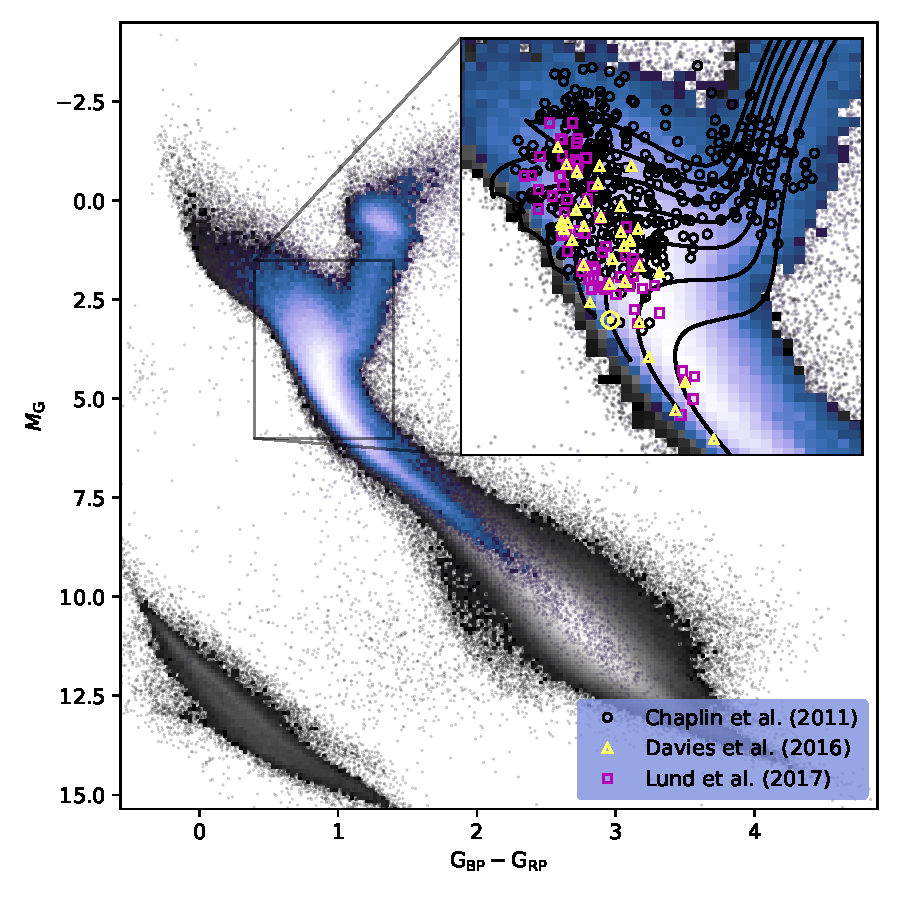
\includegraphics{figures/hr-diagram.pdf}
    \caption[Colour-magnitude diagram highlighting the region occupied by dwarf and subgiant solar-like oscillators.]{Colour-magnitude diagram highlighting the region occupied by solar-like oscillators. 
    % The data are \emph{Gaia} G, G\textsubscript{BP}, and G\textsubscript{RP} band magnitudes respectively. The absolute magnitude (\(M_\mathrm{G}\)) is calculated from \emph{Gaia} parallaxes neglecting extinction. 
    
    \emph{Main plot:} The background 2D histogram (greyscale) shows the density of \emph{Gaia} DR3 targets with parallax \(>\SI{5}{\milli\aarcsec}\) (distance \(\lesssim\SI{200}{\parsec}\)). The foreground 2D histogram (blue-purple) shows the density of all \emph{Kepler} targets in \emph{Gaia} DR3. Scattered points are shown where the density is less than 10 points per bin.
    
    \emph{Inset plot:} Stellar evolutionary tracks with solar metallicity are given by the black lines for \SIrange{0.8}{1.4}{\solarmass} in steps of \SI{0.1}{\solarmass}. The circles in the inset axes correspond to \emph{Kepler} solar-like oscillators with references given in the legend. The Sun is given by the `\(\odot\)' symbol.}
    \label{fig:hr-diagram}
\end{figure}

In Figure \ref{fig:hr-diagram}, we show a colour-magnitude diagram made using magnitudes and parallaxes from \emph{Gaia} Data Release 3 \citep[DR3;][]{GaiaCollaboration.Vallenari.ea2022}. For this illustrative plot, we have neglected the effect of extinction from dust in the interstellar medium. The background distribution shows solar-neighbourhood \emph{Gaia} sources with a parallax greater than \SI{5}{\milli\aarcsec} for context. Over-plot is the distribution of \emph{Kepler} objects cross-matched with \emph{Gaia} DR3\footnote{The cross-matched dataset was obtained from \url{https://gaia-kepler.fun}}. The densest region lies in the low- to intermediate-mass main sequence (\SIrange{0.8}{1.2}{\solarmass}) but we can also see a clear red giant branch and red clump in the upper-right of the distribution. The inset plot draws attention to the region occupied by dwarf and subgiant solar-like oscillators, where we give some examples.

\citet{Chaplin.Kjeldsen.ea2011} identified the first large catalogue of \(\sim 500\) dwarf and subgiant solar-like oscillators (black circles in Figure \ref{fig:hr-diagram}) by measuring \(\dnu\) and \(\numax\) in \emph{Kepler} data. Later, \citet{Chaplin.Basu.ea2014} determined ages, masses and radii for these stars using \(\dnu\) and \(\numax\) complemented by photometry and ground-based spectroscopy where available. The subsequent arrival of APOGEE spectroscopy allowed \citet{Serenelli.Johnson.ea2017} to revisit this sample with a more consistent set of \(\teff\) and metallicity. By comparing observations to models of stellar evolution, they found radii, masses and ages with uncertainties of around 3, 5 and 20 per cent respectively.

For a subset of these stars, the SNR was high enough to identify many individual modes. \citet{Appourchaux.Chaplin.ea2012} were among the first to publish individual mode frequencies (\(\nu_{nl}\)) for around 60 of these stars. This sample was later modelled by \citet{Metcalfe.Creevey.ea2014} who found observing individual modes doubled precision of radii, masses and ages over using \(\dnu\) and \(\numax\) alone. Around the same time, the number of confirmed exoplanets was increasing rapidly \citep{Burke.Bryson.ea2014}. This motivated a more detailed study of 35 exoplanet host stars by \citet{SilvaAguirre.Davies.ea2015} with modes identified by \citet{Davies.SilvaAguirre.ea2016}. We can see these as yellow triangles in Figure \ref{fig:hr-diagram}. The remaining best targets, referred to as the LEGACY sample, were modelled by \citet{SilvaAguirre.Lund.ea2017} using modes identified by \citet{Lund.SilvaAguirre.ea2017}. We show these as magenta squares in Figure \ref{fig:hr-diagram}.

% These targets are still being studied extensively today helium glitch \citet{Mazumdar.Monteiro.ea2014,Verma.Raodeo.ea2019}.

% While we have introduced the data used in modelling stars with asteroseismology, we have not explained how parameters like radius, mass and age are determined. In the next section, we introduce how these stars are modelled using Bayesian methodology. 

% However, there have been many sources of systematic uncertainty. Many assumptions were made in the modelling of this sample of stars. It is a perfect test case for new modelling methods. Then the plan is to apply these to future missions like Plato and Nancy Grace Roman.

\section{Modelling Stars the Bayesian Way}\label{sec:modelling-stars}

% The phrase `modelling stars' can be confusing. We often use it to describe the process of numerically simulating the physics of a star. Some examples of such simulations are one-dimensional stellar evolution codes (e.g. MESA) and three-dimensional hydrodynamical simulations \todo{e.g. other}. However, we also use the word `model' in probabilistic inference to refer to the process of generating predictions with some set of model parameters given some observed data \citep[e.g.][]{Hogg.Bovy.ea2010}. In this thesis, we prefer the phrase `modelling stars' to mean the entire process of inferring stellar parameters using a generative model. To model a given star, we may need to compute many stellar simulations, but the overall model compares these simulations to data in a probabilistic way. To avoid confusion where possible, we refer to numerical models of stars as either stellar simulations or evolutionary models.

% In some cases, stellar parameters can be estimated from observables using direct or empirical relationships. For example, mass-luminosity relation, or asteroseismic scaling relations.

% With the advent of high-precision asteroseismology for many stars, astronomers have a plethora of observables to constrain physical models of stellar evolution. 

% A la carte modelling involves producing and optimising dedicated stellar models for a given star. Many parameters can be optimised this way, but it is slow.

% Grid-based modelling involves producing a large grid of stellar models and computing the likelihood across the grid. Some examples. Assumptions must be made on approximations of stellar physics such as helium and MLT. Also overshoot, diffusion, rotation, solar abundances and opacity tables.

Modelling stars `the Bayesian way' involves estimating the probability distributions of stellar parameters (\(\vect{\theta}\)) given observed parameters (\(\vect{y}\)). For example, the parameters of interest might be the age, mass and initial fractional heavy-element abundance of the star (\(\vect{\theta} = t_\star, M, Z\)) and we might observe the effective temperature, luminosity, and large frequency spacing (\(\vect{y} = \teff, L, \Delta\nu\)). We can do this starting with Bayes' theorem for the \emph{posterior} probability density,
%
\begin{equation}
    p(\vect{\theta} \mid \vect{y}) = \frac{p(\vect{y} \mid \vect{\theta})\,p(\vect{\theta})}{p(\vect{y})},
\end{equation}
%
where \(p(\vect{y} \mid \vect{\theta})\) is the \emph{likelihood}, \(p(\vect{\theta})\) is the \emph{prior}, and \(p(\vect{y})\) is the \emph{evidence}. We should choose a prior to represent our expectation for \(\vect{\theta}\). The prior dominates if the observations are bad (i.e. have a small likelihood) and we return our current `belief' (or expectation). However, if the observations are good enough, the likelihood has more influence on the posterior and our belief is updated. As a result, we can use the Bayesian methodology to systematically update our beliefs. This provides a statistical scheme from which to build our stellar models.

Let us consider a stellar model with three parameters, \(\vect{\theta} = t_\star, M, Z\). For instance, we might want the age of a star to help date a galactic merger, or its mass to characterise an exoplanetary system. To get the probability over age given our observations, we must \emph{marginalise} over the joint posterior with respect to all other parameters. The marginal posterior probability distribution for \(t_\star\) is,
%
\begin{equation}
    p(t_\star \mid \vect{y}) = \int\limits_0^\infty \int\limits_0^1 p(\vect{\theta} \mid \vect{y}) \, \dd M \dd Z,
\end{equation}
%
where the bounds of the integral are chosen across all space for \(M\) and \(Z\). In other words, the marginal distribution involves integrating over the uncertainty in all other model parameters.

The marginal posterior distribution depends on our choice of function which maps \(\vect{\theta}\) to predict observable parameters, \(\tilde{\vect{y}} = f(\vect{\theta})\). The likelihood then compares the predictions (\(\tilde{\vect{y}}\)) with observations (\(\vect{y}\)). When modelling stars, there is no analytical form to \(f\). Instead, we use numerical simulations which take in \(\vect{\theta}\) and approximate \(\vect{y}\). For example, Modules for Experiments in Stellar Astrophysics \citep[MESA; originally developed by][]{Paxton.Bildsten.ea2011} is a one-dimensional stellar evolution code. Assuming spherical symmetry, MESA simulates the structure and evolution of a star along a one-dimensional radial slice. The code numerically solves a series of differential equations which govern the interior dynamics of the star \citep[see, e.g.][for an introduction to stellar structure and evolution]{Kippenhahn.Weigert.ea2013}. Often starting with a cloud of gas, MESA evolves the system over dynamical time steps recording physical properties at mesh points inside the star.

We can also predict oscillation mode frequencies (\(\nu_{nl}\)) with simulations. For example, the GYRE code developed by \citet{Townsend.Teitler2013} uses the output of MESA to compute oscillation modes for a given \(n\) and \(l\). While the physics of p mode propagation in the star is relatively well-known, our understanding of the atmospheric boundary conditions are not. As such, there is a known discrepancy between the simulated and observed p modes. The nature of this can lead to a systematic bias when modelled \(\dnu\) and \(\nu_{nl}\). Corrections for this effect exist \citep[e.g.][]{Ball.Gizon2014} but are still not fully understood.

The complexity of stellar models means that the marginalised posterior distributions are not analytically derivable. One solution is to estimate the posterior with numerical methods like Markov Chain Monte Carlo (MCMC). Typically, this involves exploring parameter space with multiple calls to \(f\) for different values of \(\vect{\theta}\). In the case of MCMC-based algorithms like Hamiltonian Monte Carlo (HMC) and the No U-Turn Sampler (NUTS), the gradient of \(f\) is also required. There are several open-source \textsc{Python} packages widely used to implement these algorithms, for instance \texttt{pymc} \citep{Salvatier.Wiecki.ea2016} and \texttt{numpyro} \citep{Phan.Pradhan.ea2019}.

There are some existing methods for determining stellar parameters using this Bayesian approach. As an early example, \citet{Bazot.Bourguignon.ea2008} used the MCMC algorithm to sample model parameters with on-the-fly stellar model calculation. While their method could be tailored to individual stars, it was very computationally expensive. Each proposed set of \(\vect{\theta}\) spawns a stellar simulation which evolves to a given age. Steps prior to this age may be discarded, and the simulation can take minutes to hours for each set of \(\vect{\theta}\). This was not a viable solution for modelling the large populations of stars being observed with high-precision today.

A more efficient solution is to sample a discrete grid of models \citep{Gruberbauer.Guenther.ea2012,Gruberbauer.Guenther.ea2013}. For example, a recent tool which does this is the BAyesian STellar algorithm (BASTA) developed by \citet{AguirreBorsen-Koch.Rorsted.ea2022}. The authors pre-compute and interpolate a grid of simulated stars corresponding to a set of relevant input parameters. They weight the grid points according to the prior and then compute the marginalised posterior for each model parameter. We could extend this by interpolating a grid of stellar models to approximate \(f\) itself. This is done in the Asteroseismic Inference on a Massive Scale (AIMS) pipeline by \citet{Lund.Reese2018,Rendle.Buldgen.ea2019}. However, interpolation methods can be slow. They scale poorly with dimensionality and number of points on the grid. A small subset of the grid can be used to mitigate this issue, but we want a solution which can be extended to model many stars at once.

Asteroseismology has allowed us to model stars more precisely than ever before. This has exposed systematic uncertainties in common assumptions used when computing these models \citep[e.g.][]{Tayar.Claytor.ea2022}. For instance, fractional helium abundance (\(Y\)) cannot be determined spectroscopically in cool stars. Instead, we often assume it follows a linear enrichment law \citep{Chiosi.Matteucci1982,Ribas.Jordi.ea2000,Casagrande.Flynn.ea2007}. Such a law assumes that helium is enriched in the interstellar medium linearly with metallicity. However, \citet{Lebreton.Goupil.ea2014} found that varying \(Y\) by \(\pm\,0.03\) can have \(\gtrsim \mp\,20\) per cent effect on stellar age. Therefore, assuming \(Y\) instead of incorporating it in our model leads to underestimating our uncertainty on stellar age and other correlated parameters. In Chapters \ref{chap:glitch} and \ref{chap:glitch-gp}, we will explore one way to improve inference of \(Y\) using an asteroseismic signature of helium ionisation. In the meantime, we explore a better statistical treatment of our prior on such poorly characterised parameters.

% Another assumption is the value of the mixing-length theory parameter (\(\mlt\)). This parametrises a common approximation of convective mixing used in stellar models \citep{Gough1977}. Many of the aforementioned methods assume a value of \(\mlt\) calibrated to the Sun. However, 3D hydrodynamical models have shown different values of \(\mlt\) do a better job of approximating convection for different stars \citep{Magic.Weiss.ea2015}.

% To properly model stars the Bayesian way, we need to accommodate \(Y\) and \(\mlt\) in our models. Unfortunately, the effect of these parameters on observables is degenerate. Observables are not precise enough to differentiate between the two on a star-by-star level. 

Finally, it is important that our prior represents not only our belief for individual stars, but also the population. There are many cases where we would expect stellar parameters to be correlated between stars. Not accounting for such correlations cause us to overestimate uncertainty on individual stellar parameters. For example, we believe that \(Y\) belongs to a distribution governed by chemical enrichment of the interstellar medium. Stars formed in a similar place and time should share similar chemical abundances. We can incorporate prior beliefs like this using a hierarchical Bayesian model (HBM). In the next chapter, we introduce the concept of an HBM. We explore a simple HBM in the context of astronomy and show how it can improve our estimates of stellar parameters. Following that, we present a hierarchical model on a population of dwarf and subgiant stars observed by \emph{Kepler} in Chapter \ref{chap:hmd}.

% While such a method improves upon and tackles bias in our choice of \(Y\) and \(\mlt\), there is more helium abundance information to be gained from asteroseismology. Finally, in Chapter \ref{chap:glitch}, we explore signatures of helium abundance in the oscillation modes of stars. We present a new method for characterising these glitches.

  % chapters/hbm.tex
%
% Copyright 2022 Alexander Lyttle.
%
% This work may be distributed and/or modified under the conditions of the
% LaTeX Project Public License (LPPL) version 1.3 or later.
%
% The latest version of this license is in
% https://www.latex-project.org/lppl.txt and version 1.3 or later is part of
% all distributions of LaTeX version 2005/12/01 or later.
%
%
\chapter{Hierarchical Bayesian Models}\label{chap:hbm}

\textit{In this chapter, we introduce the concept of a hierarchical Bayesian model in the context of determining stellar parameters. We use a simplified analogy for measuring distances to stars in an open cluster to demonstrate the advantages and usage of a hierarchical model in Section \ref{sec:hbm-dist}. Finally, we identify parameters which could be treated hierarchically when modelling the physical properties of many stars, priming the reader for Chapter \ref{chap:hmd}.}

\section{Introduction}

When modelling a single star, we can use a variant of Bayes' theorem (Equation \ref{eq:bayes}) to estimate the posterior probability of its parameters. We choose priors to represent our current knowledge. For example, if we observe a star in the Milky Way at random, we expect its mass to belong to an Initial Mass Function \citep[IMF; e.g.][]{Chabrier2003} without other prior knowledge. In fact, an IMF prior is an input option for BASTA \citep{AguirreBorsen-Koch.Rorsted.ea2022}. Other prior assumptions include a helium enrichment law which determines the star's initial helium abundance from its metallicity, or that its age must not be older than the universe.

Let us consider modelling a large population of stars simultaneously. For example, we may want to create a catalogue of stellar parameters to use in exoplanet and galactic research. We could treat the parameters for each star independently, repeating the modelling procedure for each star in the sample. However, we know that stars belong to population distributions like the IMF. In some cases, these population distributions are not well understood and assuming one exactly can introduce bias into our model. Instead, it could be better to let the data inform such population priors.

Hierarchical (or multi-level) Bayesian models parametrise population-level prior distributions on individual stellar parameters. These population-parameters (\emph{hyperparameters}) which govern the population must themselves have prior distributions as per the Bayesian formalisation. The hierarchical aspect comes from the distinction between hyperparameters which take one value across a population and those which vary from star-to-star. In the next section, we go through an simple example hierarchical model. Then, we discuss a few parameters which could be given the hierarchical treatment in Section \ref{sec:hbm-phys}.

\section[Stellar Distances]{Stellar Distances in an Open Cluster Analogue}\label{sec:hbm-dist}

\newcommand{\appmag}{\ensuremath{\mathrm{v}}}
\newcommand{\absmag}{\ensuremath{\mathrm{V}}}

In this section, we use the example of measuring distances to stars in an open cluster to demonstrate a hierarchical Bayesian model (HBM). This example is loosely based on the work of \citet{Leistedt.Hogg2017}, which presents a hierarchical model of the colour-magnitude diagram to improve distances from \emph{Gaia} \citep{GaiaCollaboration.Prusti.ea2016}. However, instead of considering the population distributions over magnitude and colour, we build a hierarchy over the stellar distances.

We created a dataset analogous to an open cluster of \(N_\mathrm{stars}\) stars. We gave each \(i\)-th star a dimensionless distance (\(d_i\)) from the observer drawn randomly from a normal distribution with a mean of 10 and standard deviation of 0.1. Then, we converted these to dimensionless parallax using the relation \(\varpi = 1/d\). We also gave each star an absolute visual magnitude (\(\absmag_i\)) drawn randomly from a standard normal distribution. To get a quantity proportional to apparent magnitude (\(\appmag_i\)) for each star, we used the relation \(\appmag_i = \absmag_i + 5 \log_{10} d_i\). For the purpose of this example, we ignored additional real-world effects such as extinction and reddening.

\begin{table}[tb]
    \centering
    \caption{Simulated dimensionless distance, magnitudes and parallax for \(N_\mathrm{stars}=20\) belonging to an open cluster analogue.}
    \label{tab:hbm-data}
    \begin{tabular}{r|rrrr|rr}
\toprule
 & $d_\mathrm{true}$ & $\mathrm{V_{true}}$ & $\varpi_\mathrm{true}$ & $\mathrm{v_{true}}$ & $\varpi_\mathrm{obs}$ & $\mathrm{v_{obs}}$ \\
Star &  &  &  &  &  &  \\
\midrule
0 & 9.9590 & -1.2758 & 0.10041 & 3.7153 & 0.09439 & 3.5628 \\
1 & 10.1730 & 0.3098 & 0.09830 & 5.3471 & 0.09202 & 5.3523 \\
2 & 10.1205 & -0.6844 & 0.09881 & 4.3416 & 0.10593 & 4.3648 \\
3 & 9.8957 & 0.7540 & 0.10105 & 5.7312 & 0.11552 & 5.9872 \\
4 & 10.1023 & 0.7008 & 0.09899 & 5.7229 & 0.09636 & 5.6452 \\
5 & 10.0334 & 0.2487 & 0.09967 & 5.2559 & 0.09678 & 5.2154 \\
6 & 9.9949 & 0.5171 & 0.10005 & 5.5160 & 0.09456 & 5.5110 \\
7 & 10.0877 & -3.2752 & 0.09913 & 1.7437 & 0.09919 & 1.7812 \\
8 & 10.2116 & -0.4053 & 0.09793 & 4.6402 & 0.08759 & 4.6816 \\
9 & 9.8786 & -0.4657 & 0.10123 & 4.5078 & 0.10183 & 4.5158 \\
10 & 10.0208 & -1.0131 & 0.09979 & 3.9914 & 0.12611 & 4.0295 \\
11 & 9.9049 & 1.2571 & 0.10096 & 6.2363 & 0.08160 & 6.4150 \\
12 & 9.8902 & -1.8509 & 0.10111 & 3.1251 & 0.10719 & 3.1597 \\
13 & 9.8521 & 0.8966 & 0.10150 & 5.8642 & 0.11467 & 5.8742 \\
14 & 9.9199 & 0.5401 & 0.10081 & 5.5226 & 0.09802 & 5.3892 \\
15 & 10.0848 & -0.6031 & 0.09916 & 4.4152 & 0.10617 & 4.3134 \\
16 & 9.9546 & 0.7726 & 0.10046 & 5.7627 & 0.09763 & 5.8150 \\
17 & 10.0821 & -1.2505 & 0.09919 & 3.7672 & 0.11883 & 3.6586 \\
18 & 10.0387 & -0.4488 & 0.09961 & 4.5596 & 0.07481 & 4.6057 \\
19 & 10.0174 & 1.0101 & 0.09983 & 6.0139 & 0.09255 & 5.9360 \\
\bottomrule
\end{tabular}

\end{table}

We simulated noisy observations of \(\varpi_i\) and \(\appmag_i\) by randomly drawing from a normal distribution centred on their true values with standard deviations of \(\sigma_{\appmag,i} = 0.1\) and \(\sigma_{\varpi,i} = 0.01\) respectively. We repeated this for \(N_\mathrm{stars}=20\) stars and present the true values and observables in Table \ref{tab:hbm-data}. For real-world context, the uncertainties on \(\varpi\) from \emph{Gaia} \citep{GaiaCollaboration.Prusti.ea2016} Data Release 3 \citep[][]{GaiaCollaboration.Vallenari.ea2022} are approximately \SI{0.02}{\milli\aarcsec} for stars with \emph{Gaia} G-band magnitudes of less than 15. Therefore, if our choice of \(\sigma_{\varpi,i}\) was representative of \emph{Gaia} uncertainties, then the distance to our stellar cluster would be \(\sim \SI{5}{\kilo\parsec}\). An example open cluster at this distance is NGC 6791, at \SI{4}{\kilo\parsec} \citep{Brogaard.Bruntt.ea2011}. We note that by the same comparison, our chosen spread in dimensionless distances of 0.1 corresponds to an order of magnitude more than typical cluster sizes of a few parsecs.

In Section \ref{sec:simple-model}, we describe a simple Bayesian model for determining distances and absolute magnitudes of stars in the cluster. Then, we define the HBM in Section \ref{sec:hbm-model} which incorporates a population-level distribution over distance. We outline our method for inferring model parameters in Section \ref{sec:hbm-inf} and then compare results from the models in Section \ref{sec:hbm-comp}. Finally, we explore how the HBM scales with the number of stars observed in Section \ref{sec:hbm-scale}.

\subsection{Simple Model}\label{sec:simple-model}

We started with a simxple model which treats each star independently. Using Bayes' theorem, we write the posterior probability density of the model parameters, \(d_i, \absmag_i\) given the observed parameters \(\varpi_i, \appmag_i\) as,
%
\begin{equation}
    p(d_i, \absmag_i \mid \varpi_i, \appmag_i) \propto p(\varpi_i, \appmag_i \mid d_i, \absmag_i) \, p(d_i, \absmag_i).
\end{equation}
%
The likelihood is given by \(p(\varpi_i, \appmag_i \mid d_i, \absmag_i)\) and the prior probability of the parameters is \(p(d_i, \absmag_i)\).

We modelled the likelihood as the product of normal distributions, assuming \(\varpi_i\) and \(\appmag_i\) were observed independently,
%
\begin{equation}
    p(\varpi_i, \appmag_i \mid d_i, \absmag_i) = \mathcal{N}(\varpi_i \mid d_i^{\,-1}, \sigma_{\varpi, i}^2) \, \mathcal{N}(\appmag_i \mid \absmag_i + 5\log_{10}d_i \, , \sigma_{\appmag, i}^2),\label{eq:hbm-like}
\end{equation}
%
where \(\mathcal{N}(x \,|\, \mu, \sigma^2)\) is a normal distribution over \(x\) with a mean of \(\mu\) and variance of \(\sigma^2\).

We assumed stars in the cluster were equally likely to be between a distance of 0 and 20. We also assumed the absolute magnitudes were likely to be normally distributed centred on 0 and scaled by 10. Therefore, the prior probability of the model parameters is,
%
\begin{equation}
    p(d_i, \absmag_i) = \mathcal{U}(d_i \mid 0, 20) \, \mathcal{N}(\absmag_i \mid 0, 100),
\end{equation}
%
where \(\mathcal{U}(x \,|\, a, b)\) is a uniform distribution over \(x\) from \(a\) to \(b\). We chose weakly-informative priors on the parameters, given that we know the true values for this example. However, these priors are fairly unrealistic and should be adapted to represent our expectation in real-world cases. For example, the exponential prior from \citet{Bailer-Jones.Rybizki.ea2018} would me more appropriate when observing stars radially outward from the galactic disk.

\begin{figure}[tb]
    \centering
    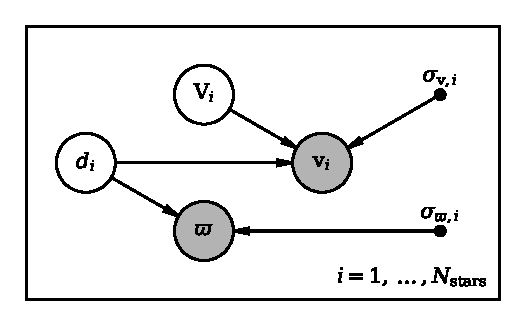
\includegraphics{figures/simple-pgm.pdf}
    \caption[Probabilistic graphical model for the simple (non-hierarchical) model]{Probabilistic graphical model for the simple (non-hierarchical) model. Parameters are given by circular nodes and connected by arrows showing the direction of dependency. Observed parameters are shaded, and fixed parameters are given by filled dots. The box represents a set of parameters belonging to the \(i\)-th star.}
    \label{fig:simple-pgm}
\end{figure}

In Figure \ref{fig:simple-pgm}, we show a probabilistic graphical model of the simple model. This shows the connections between parameters in the model. There is no hierarchy in this model because each parameter exists within the box, meaning no parameters are shared between stars. However, we know that the stellar distances are correlated. For example, it is highly unlikely that one star in the cluster is at a distance of 5 and another is at a distance of 15. If we can exploit this expectation, we could improve our prior and thus improve the inference of \(d_i\) and \(\absmag_i\).

\subsection{Hierarchical Model}\label{sec:hbm-model}

In this section, we present an HBM which includes the known correlation between distances to the stars in this open cluster analogue. We assumed the stars are all members of the same open cluster. Therefore, their distances can be modelled by some distribution. For this example, we assumed that each distance is drawn from a normal distribution characterised by new \emph{hyperparameters} \(\mu_d\) and \(\sigma_d\),
%
\begin{equation}
    d_i \sim \mathcal{N}(\mu_d, \sigma_d^2).
\end{equation}
%
The hyperparameters are so-called because they take a single value for the population of stars. Hence, the hierarchy of the model arises as some parameters represent how individual parameters are distributed in the population.

Each stellar distance, \(d_i\), is no longer independent. Hence, we modified the posterior probability distribution to account for this new correlation,
%
\begin{equation}
    p(\mu_d, \sigma_d, \vect{d}, \vect{\absmag} \mid \vect{\varpi}, \vect{\appmag}) \propto p(\vect{\varpi}, \vect{\appmag} \mid \vect{d}, \vect{\absmag}) \, p(\vect{d} \mid \mu_d, \sigma_d) \, p(\mu_d, \sigma_d, \vect{\absmag}),
\end{equation}
%
where \(p(\vect{\varpi}, \vect{\appmag} \mid \vect{d}, \vect{\absmag})\) is the likelihood --- a product over Equation \ref{eq:hbm-like},
%
\begin{equation}
    p(\vect{\varpi}, \vect{\appmag} \mid \vect{d}, \vect{\absmag}) = \prod_{i=1}^{N_\mathrm{stars}} p(\varpi_i, \appmag_i \mid d_i, \absmag_i).
\end{equation}
%
Our posterior now depends on all stars in the population, so we used bold symbols to represent the set of individual stellar parameters. For example, \(\vect{d} \equiv d_1, \dots, d_{N_\mathrm{stars}}\).

We modelled \(d_i\) as a random variable which depends on the hyperparameters. This is why our prior became the product of a conditional distribution, \(p(\vect{d} \,|\, \mu_d, \sigma_d)\) and a prior on the remaining independent parameters, \(p(\mu_d, \sigma_d, \vect{\absmag})\). We write the conditional distribution for distance as a product of normal distributions,
%
\begin{equation}
    p(\vect{d} \mid \mu_d, \sigma_d) = \prod_{i=1}^{N_\mathrm{stars}} \mathcal{N}(d_i \mid \mu_d, \sigma_d^2),
\end{equation}
%
where the prior probability distribution for \(\mu_d\) and \(\sigma_d\) is,
%
\begin{equation}
    p(\mu_d, \sigma_d) = \mathcal{U}(\mu_d \mid 0, 20) \, \mathcal{N}(\ln\sigma_d \mid - \ln 10, 1).
\end{equation}
%
We chose to use a log-normal prior for \(\sigma_d\) to ensure that the parameter is positive. The standard deviation of the prior on \(\sigma_d\) approximately corresponds to a fractional uncertainty of 100 per cent. Finally, we inherited the prior on \(\absmag_i\) from the simple model, \(p(\vect{\absmag}) = \prod_{i=1}^{N_\mathrm{stars}} \mathcal{N}(\absmag_i \,|\, 0, 100)\).

\begin{figure}[tb]
    \centering
    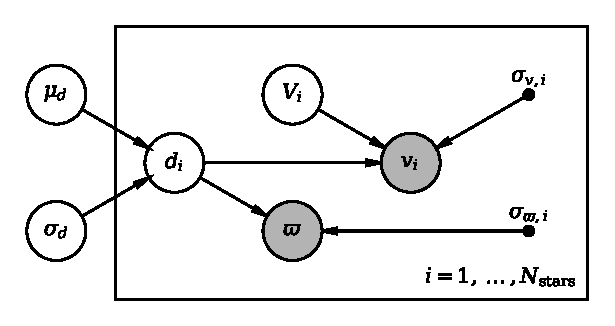
\includegraphics{figures/hbm-pgm.pdf}
    \caption[Probabilistic graphical model for the hierarchical model]{Probabilistic graphical model extension of Figure \ref{fig:simple-pgm} but for the HBM. The hyperparameters exist outside of the box to show that they are the same across the population of stars.}
    \label{fig:hbm-pgm}
\end{figure}

We show the probabilistic graphical model of the HBM in Figure \ref{fig:hbm-pgm}. Here, we see how all individual stellar parameters depend on \(\mu_d\) and \(\sigma_d\). This is a simple extension of Figure \ref{fig:simple-pgm}, but with parameters existing outside of the box to illustrate the model hierarchy. We can imagine extending this framework to multiple levels, or adding additional hyperparameters.

\subsection{Inferring the Model Parameters}\label{sec:hbm-inf}

To infer the model parameters, we need to calculate the marginalised posterior distributions for each parameter. We could obtain these analytically by integrating the full posterior distribution over all model parameters except for the parameter of interest. Alternatively, we can approximate the marginalised posterior using a Markov Chain Monte Carlo (MCMC) sampling algorithm. We chose the latter approach because it is scalable to more complicated models where the marginalisation is not analytically solvable.

We used the No U-Turn Sampler \citep[NUTS;][]{Hoffman.Gelman2014} as implemented in the \textsc{NumPyro} Python package \citep{Phan.Pradhan.ea2019,Bingham.Chen.ea2019} to sample from the approximate posterior distribution for both models. We took 1500 samples, with the first 500 samples discarded as `warmup' steps, repeated for 10 MCMC chains. We increased the target accept probability from 0.8 to 0.98 for the HBM, to minimise the number of divergences encountered during sampling. The resulting marginalised posterior samples amounted to \num{10000} per parameter.

\subsection{Comparing the Models}\label{sec:hbm-comp}

\begin{figure}[p]
    \centering
    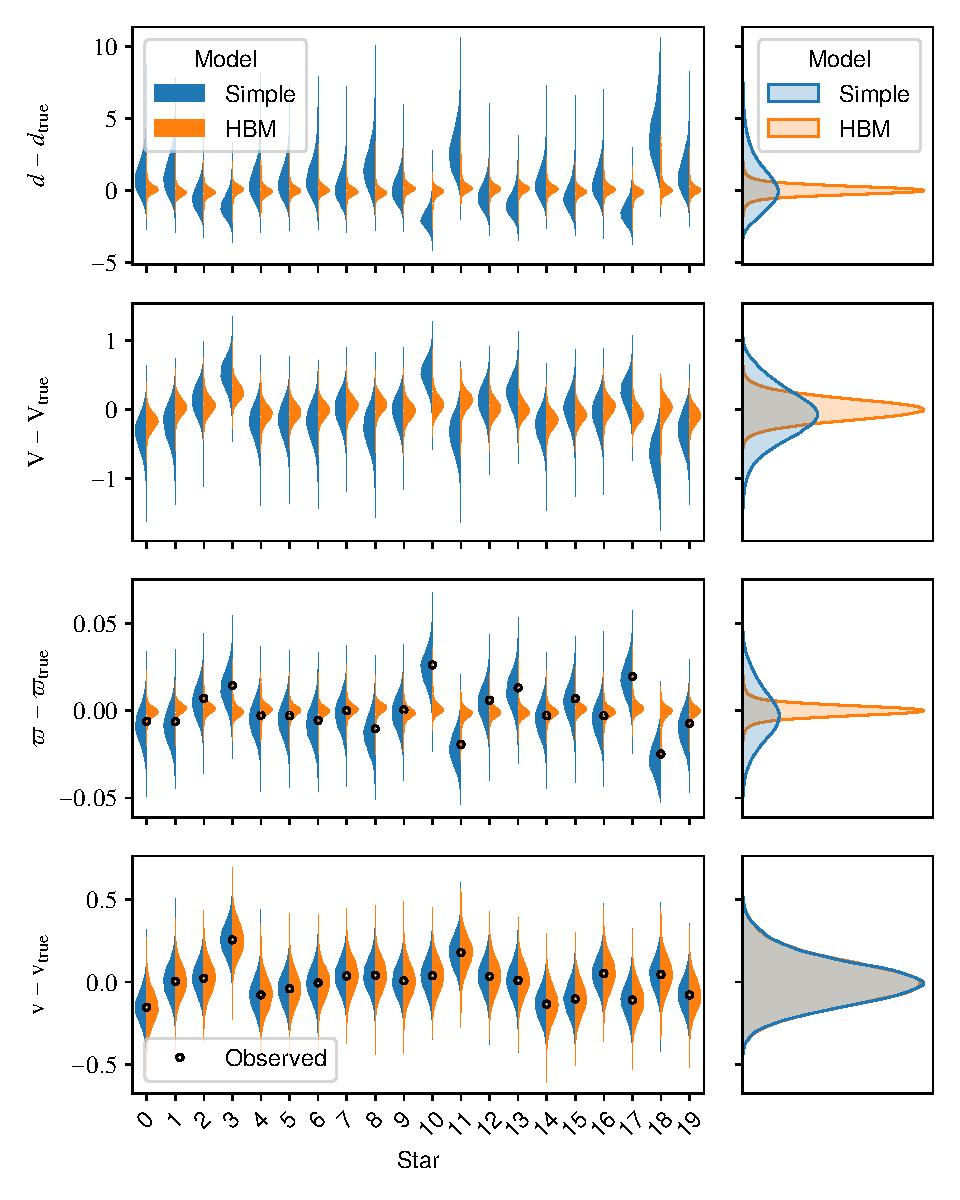
\includegraphics{figures/hbm-results.pdf}
    \caption[Plots comparing results from the simple model to the HBM]{Plots comparing results from the simple model (\emph{blue}) to the HBM (\emph{orange}). \emph{Left column:} Split violin-plots showing the difference between marginalised posterior distributions for the parameters and their true values. \emph{Right column:} Kernel density estimates of the parameter-truth differences over all \(N_\mathrm{stars}\). Observed values of the parameters are given by empty black circles.}
    \label{fig:hbm-results}
\end{figure}

We compared the difference between model parameters and their true values in Figure \ref{fig:hbm-results}. The HBM showed clear improvement over the simple model in all parameters except for apparent magnitude. Pooling the distances shrank their standard deviations by about one third and converged on their true values. This had the effect of removing the observational noise on \(\varpi\), as we can see the posterior predictions for parallax also approached their true values. Since apparent magnitude depended on both \(d\) and \(\absmag\), better distances also improved the absolute magnitudes.

% \todo{Hand-wavy why apparent magnitude saw no improvement was because the observational noise on parallax had a larger impact on the distance than with apparent magnitude. \(\appmag \propto \log_{10}d\), whereas \(\varpi = d^{-1}\). Additionally, the fractional uncertainty on parallax was greater than that of apparent magnitude. The noise budget is dominated by the parallax, so this is the first to be improved by better distances. \(\sigma_\varpi/\varpi = \sigma_d \varpi\), but \(\sigma_\appmag / \appmag \propto \sigma_d \varpi / \appmag\)}

\begin{figure}
    \centering
    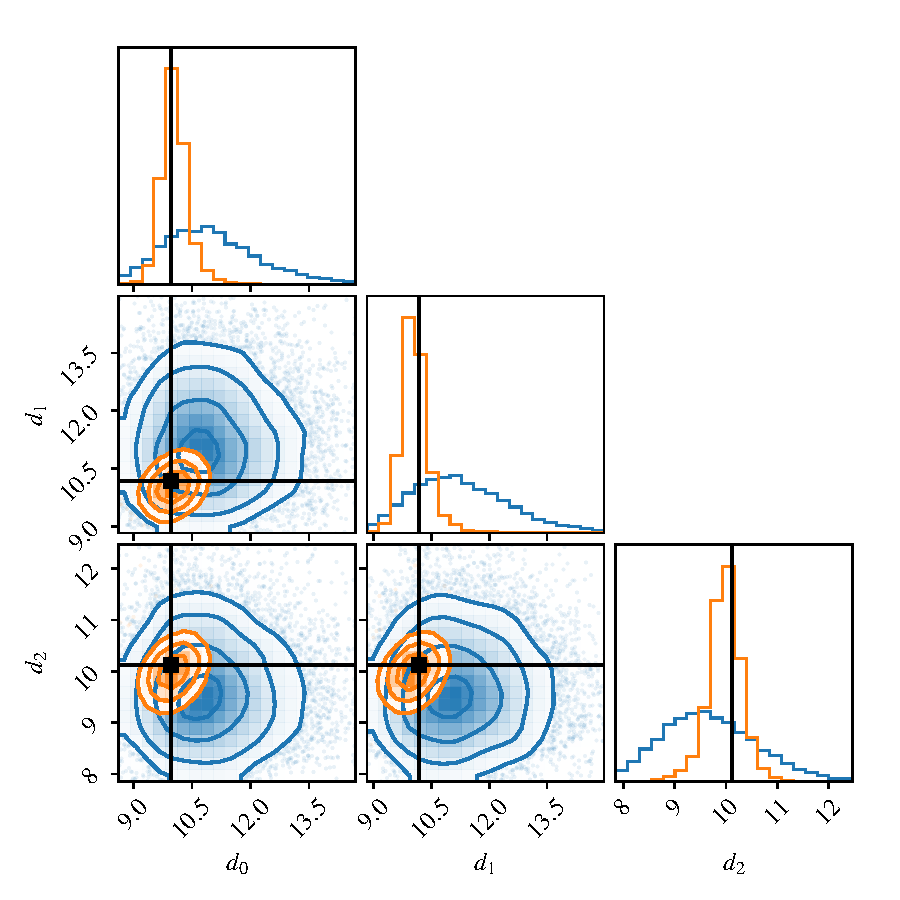
\includegraphics{figures/hbm-dist-corr.pdf}
    \caption[A corner plot showing the marginalised and joint posterior distributions of the distance to the first three stars]{A corner plot showing the marginalised and joint posterior distributions of the distance to the first three stars. The simple model is shown in \emph{blue} and the HMB is shown in \emph{orange}. The true values are given by the \emph{black} lines. The range of the distributions are limited to 98 per cent of the simple model's marginalised posteriors.}
    \label{fig:hbm-corr}
\end{figure}

In Figure \ref{fig:hbm-corr}, we compared the joint and marginalised posteriors of the distance to a few of the stars. The HBM found distances to higher precision, with typical standard deviations of \(s_{d,i} \approx 0.35\) compared to \(s_{d,i} \approx 1.2\) from the simple model. We also noticed a one-to-one correlation between \(d\) present in the HBM but not in the simple model. This was a result of the correlation introduction by the population-prior on \(d\). For each distance, we saw how a lower value in one corresponded to a lower value for the others. This represents our belief that cluster members should share a similar distance. On the other hand, the simple model suggested it was, for example, just as likely to find two stars at distances of 9 and 12 as it would for both to be at a distance of 11.

\begin{figure}[tb]
    \centering
    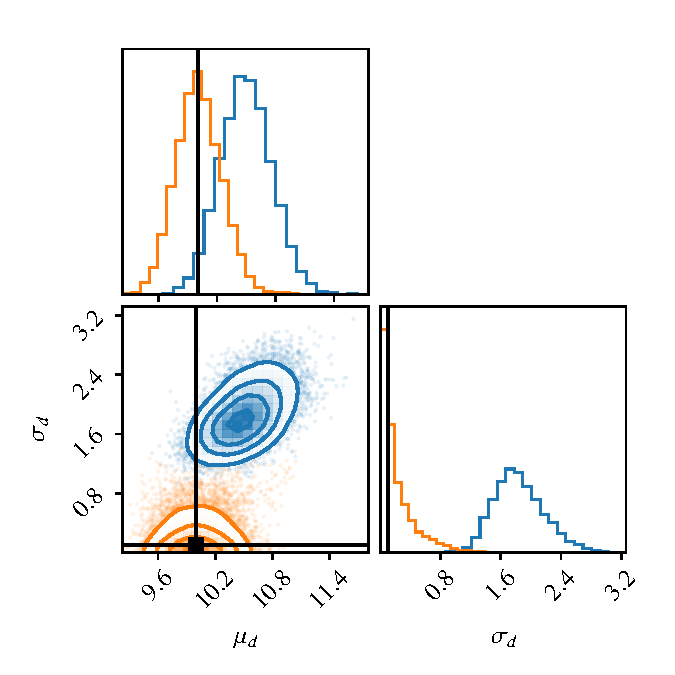
\includegraphics{figures/hbm-global.pdf}
    \caption[The joint and marginalised posterior distributions for the mean and standard deviation of stellar distances in the cluster]{The joint and marginalised posterior distributions for the mean (\(\mu_d\)) and standard deviation (\(\sigma_d\)) of stellar distances in the cluster. The simple model is shown in \emph{blue} and the HMB is shown in \emph{orange}. The true values are given by the \emph{black} lines.}
    \label{fig:hbm-global}
\end{figure}

One consequence of the HBM was that it parametrised the population mean (\(\mu_d\)) and standard deviation (\(\sigma_d\)) of the distances to stars in the cluster independently from the observed noise. For the simple model, we estimated \(\mu_d\) and \(\sigma_d\) by taking the sample mean and standard deviation of distances in the cluster for each posterior sample. We compared the resulting posterior distributions for \(\mu_d\) and \(\sigma_d\) from the two models in Figure \ref{fig:hbm-global}. We found the mean distance from the simple model was \(\mu_d = 10.50 \pm 0.27\), whereas the HBM was more accurate with \(\mu_d = 10.01 \pm 0.24\). We also found the simple model massively overestimated the standard deviation of cluster distances with \(\sigma_d = 1.815_{-0.293}^{+0.360}\), compared to the HBM's more accurate value of \(\sigma_d = 0.131_{-0.088}^{+0.280}\). The simple model cannot easily distinguish between the uncertainty on individual distances and the spread of the population.

\subsection{Scaling with the Number of Stars}\label{sec:hbm-scale}

To test how the model scales with number of stars, we repeated the HBM method for different \(N_\mathrm{stars}\). We randomly generated true and observed parameters in the same way as described at the beginning of \ref{sec:hbm-dist} for 320 stars. The observables were different to the last section, but drawn from the same distributions. We then sampled from the HBM for the first 20, 80 and 320 stars. These represented ratios in \(N_\mathrm{stars}^{1/2}\) of \(1\), \(2\) and \(4\) respectively.

\begin{figure}[tb]
    \centering
    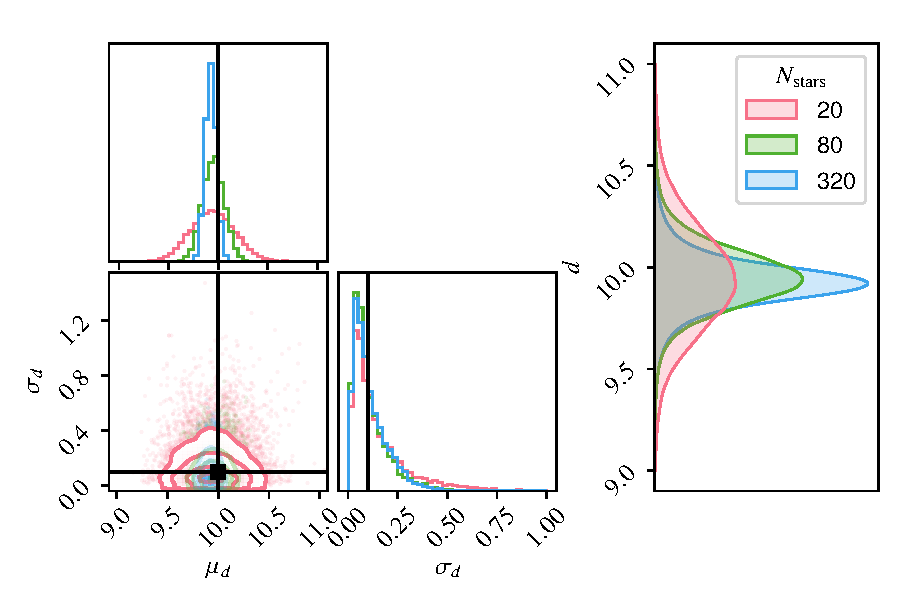
\includegraphics{figures/hbm-extended.pdf}
    \caption{Joint and marginalised posterior distributions from the HBM for 20, 80 and 320 stars.}
    \label{fig:hbm-extended}
\end{figure}

Figure \ref{fig:hbm-extended} shows how the distance estimates improved with increasing number of stars observed, \(N_\mathrm{stars}=(20,80,320)\). Unsurprisingly, the standard deviation on \(\mu_d\) decreased by a factor of \(N_\mathrm{stars}^{1/2}\) each time, with \(s_{\mu_d} \approx (0.24, 0.12, 0.06)\). We also expected a similar reduction in uncertainty for individual distances, albeit limited by the observational noise. Typical standard deviations for \(d_i\) were \(s_{d,i} \approx (0.30, 0.17, 0.15)\). As expected, the distance uncertainties also halved from \(20\) to \(80\) stars. However, this effect lessened with 320 stars. This demonstrated the method is still limited by the error budget across all observed parameters. Despite this, the HBM proved to be a useful way of getting more information from a limited number of noisy observations. 

\section[Stellar Properties]{Inferring Physical Properties of Stars}\label{sec:hbm-phys}

We have seen how a simple HBM can be used to improve the distances and absolute magnitudes of stars in a cluster analogue. This kind of model only represents part of the puzzle for determining ages, masses, and radii in a population of stars. In these Bayesian stellar models (discussed previously in Section \ref{sec:modelling-stars}) we have more parameters which could be considered hierarchically. In this section, we discuss a few possible population distributions which could form a hierarchical model of stellar physics.

\paragraph{Mass} As mentioned in the introduction to this chapter, an IMF may be used as a prior on the mass of a star. If modelling stars with masses spanning a couple of orders of magnitude, it makes sense to draw their masses from an IMF. To make this hierarchical, we would parametrise the IMF as a conditional distribution which informs individual stellar masses. This way, the population of stars constrains the IMF while in-turn sharing information. In this thesis, we only consider stars in a narrow mass range (\SIrange{0.8}{1.2}{\solarmass}) where the IMF does not change much. However, a mass hierarchy like this may be useful in future work.

\paragraph{Age} We do not expect a star to be older than the universe. This makes the age of the universe a natural upper limit to a prior on stellar age. There are also populations of stars where we expect the age to be tightly related. For example, star systems like binaries and clusters are expected to have been formed at a similar time. Similarly to the distances in Section \ref{sec:hbm-dist}, a hierarchical model in age would parametrise the mean and variance of ages in these systems and in-turn improve other connected model parameters. This sort of analysis could be extended to find mixtures of age distributions in the galaxy which could indicate mergers \citep[e.g. \emph{Gaia}-Enceladus;][]{Helmi.Babusiaux.ea2018}. However, we do not further consider a HBM in age this in this work.

\paragraph{Chemical Abundances} Unlike mass and age, surface abundances of stars can be measured directly with spectroscopy. However, not all abundances are easily measured. For example, helium ionises below the surface of the cool stars being studied in this work. Also, diffusion and settling of elements during stellar evolution means surface abundances differ from formation to time of observation. Similarly to age, we can expect clusters of stars to share initial abundances. However, the distribution of abundances in the Milky Way may also be parametrised. As stars evolve they convert hydrogen into helium and heavier elements. Supernovae enrich the galaxy with these elements monotonically, which go on to constitute new stars. A hierarchical model could include this assumption to tie the abundance of helium to heavier elements.

\paragraph{Approximations of Stellar Physics} A hierarchical model need not be limited to real physical parameters. In stellar modelling, we often approximate stellar physics with \emph{pseudo}-physical parameters. For example, convective energy transfer is approximated by the mixing-length theory \citep[MLT;][]{Gough1977} parametrised by \(\mlt\). The value of \(\mlt\) which best models a star is likely to vary with other stellar parameters. It's effect on observables is small making \(\mlt\) difficult to constrain on a star-by-star basis. Hence, a hierarchical model would be able to condition individual values of \(\mlt\) on its population distribution. A distribution over pseudo-physical parameters is less intuitive, yet the HBM would allow us to build one empirically. In addition to the initial helium abundance, \(\mlt\) is modelled hierarchically in Chapter \ref{chap:hmd}.

  % chapters/lyttle21.tex
%
% Copyright 2023 Alexander Lyttle.
%
% This work may be distributed and/or modified under the conditions of the
% LaTeX Project Public License (LPPL) version 1.3 or later.
%
% The latest version of this license is in
% https://www.latex-project.org/lppl.txt and version 1.3 or later is part of
% all distributions of LaTeX version 2005/12/01 or later.
%
%
\chapter[Hierarchically Modelling Dwarf and Subgiant Stars]{Hierarchically Modelling \emph{Kepler} Dwarfs and Subgiants to Improve Inference of Stellar Properties with Asteroseismology}\label{chap:hmd}

\textit{%
    In this chapter, I present the entirety of \citet{Lyttle.Davies.ea2021} with minor modification. I confirm that all writing is my own except for the description of stellar models and input physics in Section \ref{sec:grid} which was written by Tanda Li\footnote{Institute for Frontiers in Astronomy and Astrophysics, Beijing Normal University, Beijing 102206, China}. In this work, we created a hierarchical Bayesian model to pool information about the distribution of helium abundance (\(Y\)) and mixing-length-theory parameter (\(\mlt\)) in a population of dwarf and subgiant solar-like oscillators.
}

\section{Introduction}

%%%%%%%%%%%%%%%%%%%%%%%%%%%%%%%%%%%%%%%%%%%%%%%%%%

%%%%%%%%%%%%%%%%%% INTRODUCTION %%%%%%%%%%%%%%%%%%

The inference of stellar ages, masses, and radii has improved through the use of asteroseismology in recent years \citep[e.g. see the review by][]{Chaplin.Miglio2013}. Measuring the oscillation modes in stars using photometric time series data, from missions such as \emph{CoRoT} \citep{Baglin.Auvergne.ea2006}, \emph{Kepler} \citep{Borucki.Koch.ea2010}, and \emph{TESS} \citep{Ricker.Winn.ea2015} has given us new insights into the structure and evolution of stars \citep{Garcia.Ballot2019}. Recent examples include a deeper understanding of stellar structure \citep{Verma.Raodeo.ea2017}, chronology of a Milky Way merger \citep{Chaplin.Serenelli.ea2020}, and classifying exoplanetary systems \citep{Huber.Chaplin.ea2019, Tayar.Claytor.ea2020}. Several studies used grids of stellar models with constraints from asteroseismology to produce catalogues of precise stellar parameters \citep{Pinsonneault.Elsworth.ea2014, SilvaAguirre.Lund.ea2017}. However, with increasing precision on fundamental parameters inferred from stellar models with asteroseismology, we should take extra care to ensure that we are accounting for uncertainty in our choice of stellar physics.

Typically, stars are modelled on a star-by-star basis with estimates of stellar properties including some assumptions handled by simple scaling relations and solar calibrations. For instance, a helium ($Y$) to heavy-element ($Z$) enrichment ratio ($\Delta Y / \Delta Z$) and mixing-length theory parameter ($\mlt$) are often assumed. However, there has been little effort to account for the population distribution of such quantities. Assuming values for $Y$ and $\mlt$ can result in inaccurate inference and systematics on the inferred stellar parameters \citep{Valle.DellOmodarme.ea2015}. Independently modelling $Y$ and $\mlt$ can also be computationally demanding and requires high-precision observations in order to return meaningful stellar properties.

In this work, we apply a new method to determine stellar properties for a sample of \emph{Kepler} dwarfs and subgiants using a hierarchical Bayesian model (HBM). With an HBM, we introduce population-level distributions for $Y$ and $\mlt$ to encode prior information throughout the sample. We will show that when an HBM is used, we can increase the precision of inferred masses, radii, and ages despite increasing the number of free parameters.

The use of HBMs has been demonstrated in other areas of stellar astrophysics to reduce individual parameter uncertainties by encoding prior information about the distribution of the parameter in a population. For example, HBMs have been used with data from \emph{Gaia}, improving distance measures \citep{Leistedt.Hogg2017, Anderson.Hogg.ea2018} and calibrating the red clump as a standard candle \citep{Hawkins.Leistedt.ea2017, Chan.Bovy2020} using asteroseismology \citep{Hall.Davies.ea2019}. In other instances, HBMs have been used to infer binary-star and exoplanet eccentricities \citep{Hogg.Myers.ea2010}, obliquity of transit systems \citep{Morton.Winn2014}, stellar inclination with asteroseismology \citep{Campante.Lund.ea2016, Kuszlewicz.Chaplin.ea2019}, and the age-metallicity relation of the solar neighbourhood \citep{Feuillet.Bovy.ea2016}.

To describe the distribution of $Y$ in this work, we assume a linear helium enrichment law characterised by freely varied population parameters: the gradient given by $\Delta Y / \Delta Z$, the primordial helium abundance at $Z=0$ ($Y_P$) and an intrinsic spread in helium ($\sigma_Y$). There have been many studies to determine a linear enrichment law, from modelling eclipsing binaries \citep{Ribas.Jordi.ea2000} to spectroscopy of galactic H\,\textsc{ii} regions \citep{Balser2006}. Values of $\Delta Y / \Delta Z$ have also been determined for samples of main sequence (MS) stars \citep{Casagrande.Flynn.ea2007}, open clusters \citep{Brogaard.VandenBerg.ea2012}, and more recently with asteroseismology using individual oscillation frequencies \citep{SilvaAguirre.Lund.ea2017} and the glitch due to the second helium ionisation zone \citep{Verma.Raodeo.ea2019}. In these studies the value of the enrichment ratio was typically inferred to be $1 \lesssim \Delta Y / \Delta Z \lesssim 3$. However, helium enrichment is unlikely to be exactly linear with metallicity and may depend on other chemical abundances \citep{West.Heger2013} or the location of the star in the Milky Way \citep{Frebel2010}. Therefore, we account for some deviation from the linear law by introducing $\sigma_Y$. Moreover, our method may be adapted to different helium enrichment priors in future work.

The widely used mixing-length theory (MLT) of convection, parametrised by $\mlt$, has been tested throughout the Hertzsprung-Russell (HR) diagram with 3D hydrodynamical simulations \citep{Trampedach.Stein.ea2014, Magic.Weiss.ea2015} and asteroseismology \citep{Tayar.Somers.ea2017, Viani.Basu.ea2018, Li.Bedding.ea2018} with values in the range $0.8 \lesssim \mlt/\alpha_{\mathrm{MLT}, \odot} \lesssim 1.2$ where $\alpha_{\mathrm{MLT}, \odot}$ is the value calibrated to the Sun. However, in many grids of stellar models, a constant value calibrated to reproduce the Sun is assumed. This can lead to systematic uncertainties in stellar ages due to the effects of variable mixing depending on the mixing length. The MLT approximates convective mixing, and thus we expect the value of $\mlt$ to vary from star-to-star due to various effects, from changes in chemical composition to other sources of mixing described poorly by MLT. The investigation of more complex $\mlt$ distributions is beyond the scope of this work. Instead, we experiment with two prior assumptions for $\mlt$ in the population. The first assumes $\mlt$ is normally distributed in our sample with a spread ($\sigma_\alpha$) to account for the aforementioned variation in $\mlt$. The second assumes $\mlt$ is constant throughout the sample.

Our HBM requires a way to map from the stellar initial (or bulk) properties to predict observables. We can achieve this with a large grid of stellar evolutionary models. However, a discrete grid can produce inaccurate posterior distributions, limited to the grid resolution. Increasing the resolution is computationally demanding, especially when scaling to higher input dimensions. One solution is to interpolate the stellar models, as is common in the isochrone-fitting method \citep[see e.g.][]{Berger.Huber.ea2020}. However, interpolation can become computationally expensive at high input dimensions and grid size, and evaluating the likelihood using modern Bayesian sampling techniques is slow. Therefore, we use machine learning to map stellar model inputs to observables to provide a fast way to sample the HBM. In this work, we train an artificial neural network (ANN) on a large grid of stellar models. There have been similar applications of ANNs in asteroseismology \citep{Verma.Hanasoge.ea2016, Bellinger.Angelou.ea2016, Hon.Stello.ea2017, Hon.Stello.ea2018a, Hendriks.Aerts2019} but not yet in the context of an HBM. Using the machine learning speed-up, we demonstrate a scalable method for obtaining fundamental stellar parameters.

In Section \ref{sec:data}, we describe the data for the sample of 81 \emph{Kepler} dwarfs and subgiants studied in this work. We then present the methods in Section \ref{sec:meth} for which we produced a large grid of stellar evolutionary models to use as training data for an ANN. We use the ANN as an emulator in a series of statistical models described in Section \ref{sec:hbm} to model the sample and present our results in Section \ref{sec:res}. Finally, in Section \ref{sec:dis} we discuss the results from each model and compare them to results for the sample of stars in the literature.

\section{Data}\label{sec:data}

%%%%%%%%%%%%%%%%%%%%%%%%%%%%%%%%%%%%%%%%%%%%%%%%%%

%%%%%%%%%%%%%%%%%%%%%% DATA %%%%%%%%%%%%%%%%%%%%%%

For this study, we selected the sample of 415 stars from the first APOKASC catalogue of dwarfs and subgiants \citep[][hereafter \serenelli]{Serenelli.Johnson.ea2017}. This sample provides an extensive set of dwarfs and subgiant stars with asteroseismic detections observed by the \emph{Kepler} mission. \citetalias{Serenelli.Johnson.ea2017} used grid-based modelling to determine the ages ($\tau$), masses ($M$), radii ($R$), and surface gravity ($\log g$) of stars in the sample, using global asteroseismic parameters, effective temperature ($\teff$), and metallicity ($\metallicity$) as inputs.

Using five independent pipelines, \citetalias{Serenelli.Johnson.ea2017} determined values for global asteroseismic parameters --- the large frequency separation $\dnu$ and the frequency at maximum power, $\numax$ with median uncertainties of 1.7 per cent and 4 per cent respectively. We chose to adopt the $\dnu$ determined in their work as inputs for our method. They also used $\metallicity$ published in Data Release 13 \citep[DR13;][]{Albareti.AllendePrieto.ea2017} of the APOGEE stellar abundances pipeline \citep[ASPCAP;][]{GarciaPerez.AllendePrieto.ea2016} with uncertainties of \SI{0.1}{\dex}. For their preferred set of results, they adopted $\teff$ from the Sloan Digital Sky Survey (SDSS) \emph{griz}-band photometry \citep{Pinsonneault.An.ea2012} with a median uncertainty of \SI{70}{\kelvin}.

We removed more evolved stars from the APOKASC sample by cutting those with $\log g < \SI{3.8}{\dex}$. We then kept stars within 1-$\sigma$ of $-0.5 < \metallicity < \SI{0.5}{\dex}$ to remove metal-poor stars. Main sequence stars with $M \gtrsim \SI{1.2}{\solarmass}$ are understood to have a convective, hydrogen-burning core, with some dependence on the chemical composition and choice of stellar physics \citep{Appourchaux.Antia.ea2015}. Stellar models with a convective core require the treatment of extra stellar physics such as overshooting, which is beyond the scope of this work. Therefore, we keep only stars with masses within 1-$\sigma$ of \SIrange{0.8}{1.2}{\solarmass} from the preferred set of results of \citetalias{Serenelli.Johnson.ea2017}.

Following cuts to the sample, we adopted updated ASPCAP spectroscopic metallicities, \metallicity, from Data Release 14 \citep[DR14;][]{Blanton.Bershady.ea2017} which had a median uncertainty of \SI{0.07}{\dex}. We also chose to adopt $\teff$ from the same catalogue to be internally consistent. We note that our chosen effective temperature scale is offset from the photometric temperature scale of \citetalias{Serenelli.Johnson.ea2017} by approximately $- \SI{170}{\kelvin}$, with a dispersion of $\sim \SI{120}{\kelvin}$ corresponding to typical uncertainties on the individual temperatures. The median uncertainty in our adopted ASPCAP $\teff$ was \SI{125}{\kelvin}.

To provide a means of calculating luminosities, we used \emph{Gaia} Data Release 2 (DR2) parallaxes \citep{GaiaCollaboration.Prusti.ea2016, GaiaCollaboration.Brown.ea2018}. We cross-matched the remaining sample with the DR2 catalogue, taking the nearest neighbours within a 4 arcsec radius. Although DR2 parallaxes have improved upon the DR1 values at the time of \citetalias{Serenelli.Johnson.ea2017}, there was still evidence for a zero-point offset \citep{Lindegren.Hernandez.ea2018}. We adopted a global offset of \SI{0.05}{\milli\aarcsec}, in the sense that DR2 parallaxes were underestimated, representative of values obtained in the literature using \textit{Kepler} field stars \citep[see e.g.][]{Zinn.Pinsonneault.ea2019, Hall.Davies.ea2019} and through other methods \citep[see e.g.][]{Riess.Casertano.ea2018, Chan.Bovy2020}. We then cross-matched our sample with the Two-Micron All Sky Survey \citep[2MASS;][]{Skrutskie.Cutri.ea2006} to obtain \emph{K\textsubscript{S}}-band (\SI{2.16}{\micro\metre}) photometry.

We determined luminosities, $L$ for the sample using the direct method of \textsc{isoclassify} \citep{Huber.Zinn.ea2017, Berger.Huber.ea2020} with \emph{K\textsubscript{S}}-band photometry, \emph{Gaia} DR2 parallaxes, ASPCAP $\metallicity$ and $\teff$, and asteroseismic $\log g$ as inputs. This involved computing absolute \emph{K\textsubscript{S}}-band magnitudes using the \emph{Gaia} DR2 parallaxes and extinctions determined by the 3D galactic reddening maps of \citet{Green.Schlafly.ea2018}. We determined absolute bolometric magnitudes by interpolating the MIST bolometric correction tables as a function of $\teff$, $\log g$ and $\metallicity$ \citep{Dotter2016, Choi.Dotter.ea2016}. We adopted the uncertainty of \SI{0.02}{\magnitude} assumed by \textsc{isoclassify} for both the extinctions and bolometric corrections, corresponding to typical systematic errors in extinction maps and bolometric fluxes \citep[e.g.][]{Zinn.Pinsonneault.ea2019a,Tayar.Claytor.ea2020}. We obtained luminosities for the sample with a median uncertainty of 3.4 per cent.

\begin{table*}
	\centering
	\caption[The observables and their respective uncertainties for 5 stars in the sample of 81 stars.]{The observables and their respective uncertainties for 5 stars in the sample of 81 stars. The whole table is available as supplementary material for the original article \citep{Lyttle.Davies.ea2021}.}
	\label{tab:data}
	\begin{tabular}{lcccc}
\toprule
Name & $\teff\,(\si{\kelvin})$ & $L\,(\si{\solarluminosity})$ & $\dnu\,(\si{\micro\hertz})$ & $\metallicity_\mathrm{surf}\,(\si{\dex})$ \\
\midrule
  KIC10079226 &            $5929\pm125$ &              $1.571\pm0.049$ &             $116.04\pm0.73$ &                           $0.159\pm0.074$ \\
  KIC10215584 &            $5667\pm119$ &              $1.637\pm0.063$ &             $115.16\pm2.83$ &                           $0.043\pm0.069$ \\
  KIC10319352 &            $5456\pm107$ &              $1.848\pm0.056$ &              $78.75\pm1.73$ &                           $0.265\pm0.065$ \\
  KIC10322381 &            $6147\pm149$ &              $2.445\pm0.079$ &              $86.64\pm6.57$ &                          $-0.317\pm0.079$ \\
  KIC10417911 &            $5628\pm110$ &              $3.408\pm0.115$ &              $56.14\pm2.10$ &                           $0.336\pm0.068$ \\
\bottomrule
\end{tabular}

\end{table*}

\begin{figure}[tb]
    \centering
    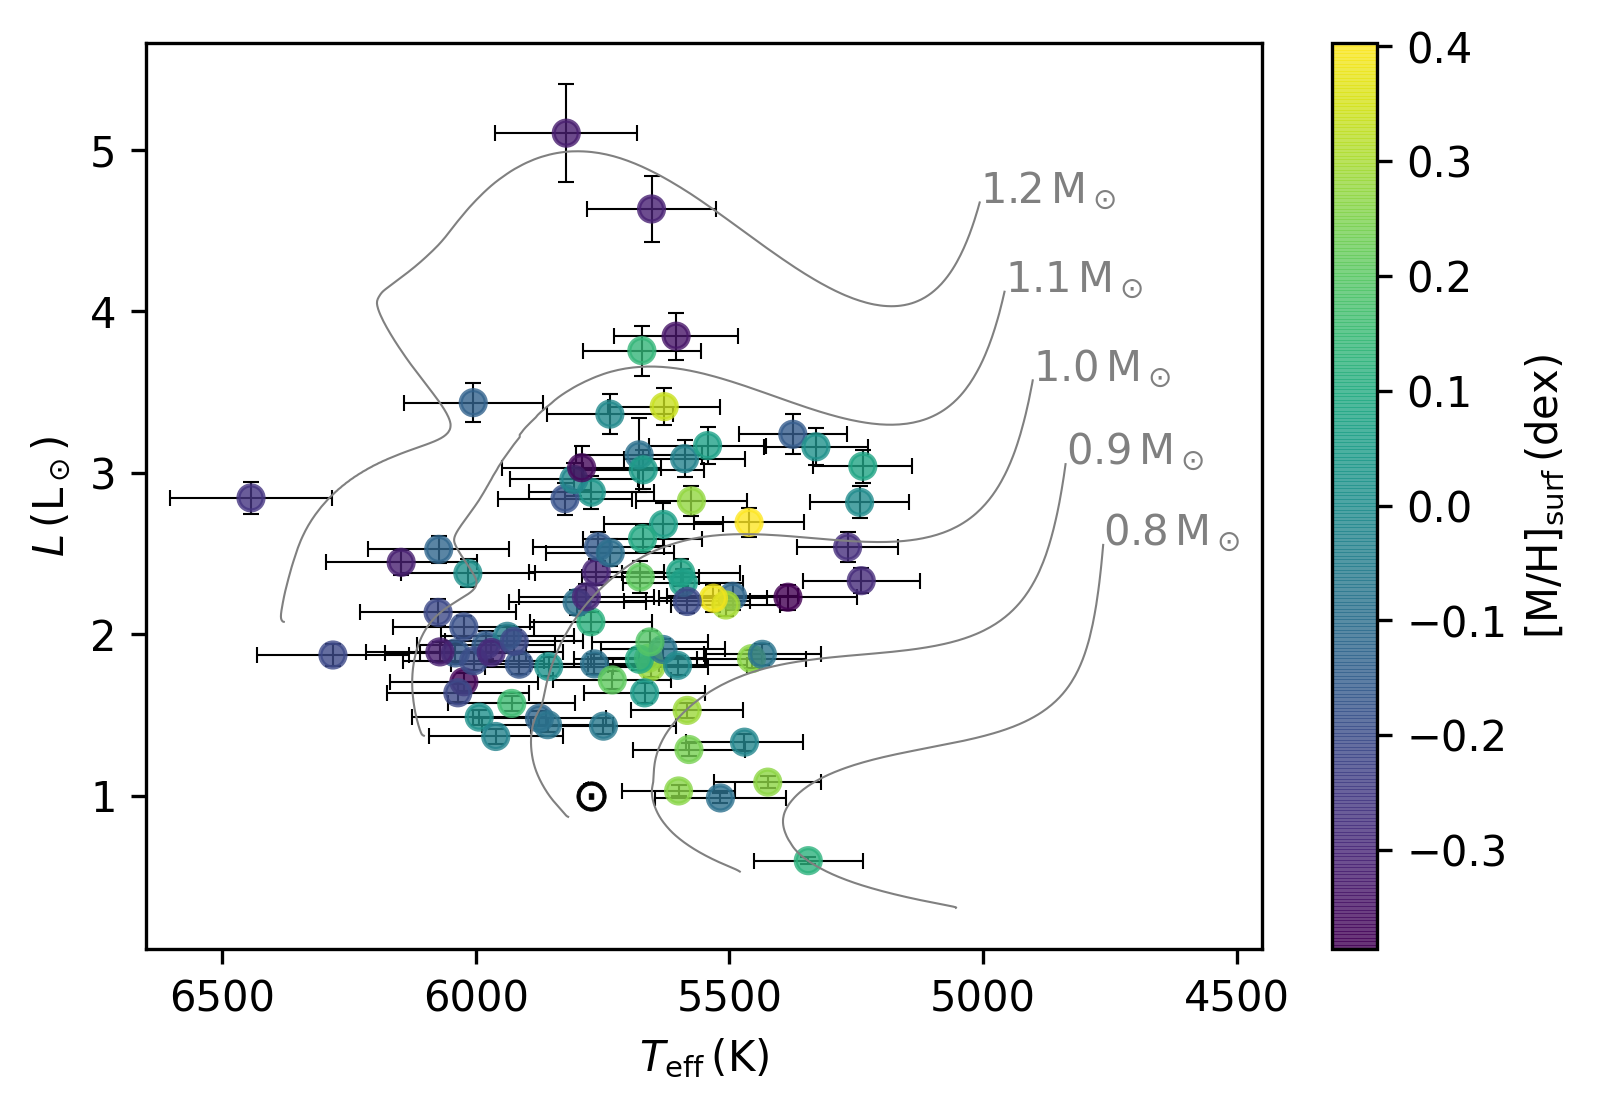
\includegraphics{figures/context.png}
    \caption[The luminosity against effective temperature of the sample of 81 \emph{Kepler} dwarfs and subgiants studied in this work.]{The luminosity, $L$ against effective temperature, $\teff$ of the sample of 81 \emph{Kepler} dwarfs and subgiants studied in this work. Each stars is coloured according to metallicity. The grey lines depict evolutionary tracks with $\metallicity_\mathrm{init}=\SI{0.0}{\dex}$, $Y_\mathrm{init}=0.28$ and $\mlt=1.9$ for different stellar masses. The current position of the Sun is shown by the $\odot$ symbol.}
    \label{fig:data}
\end{figure}

The final sample comprised 81 stars for which we had complete data for $\teff$, $\metallicity$, $\dnu$, and $L$ to use as inputs for our stellar modelling method --- see Table \ref{tab:data}. In Fig. \ref{fig:data}, we show the HR diagram for the sample plot in context with a series of stellar evolutionary tracks at solar metallicity.

\section{Methods}\label{sec:meth}

%%%%%%%%%%%%%%%%%%%%%%%%%%%%%%%%%%%%%%%%%%%%%%%%%%

%%%%%%%%%%%%%%%%%%%% METHODS %%%%%%%%%%%%%%%%%%%%%

Firstly, we used a stellar evolutionary code to compute a grid of models to predict observable quantities (see Section \ref{sec:grid}). Subsequently, we trained an ANN on the grid of stellar models to map input parameters to output observables (see Appendix \ref{sec:ann} for further details). We then constructed three Bayesian models in Section \ref{sec:hbm} which each sampled the trained ANN to estimate stellar fundamental parameters as described in Section \ref{sec:sampling}. Evaluation of the ANN gradient is required during training. Consequently, estimating the gradient of the model likelihood is fast and simple when the observables are generated by an ANN. Hence, we open up the possibility of using a Hamiltonian Monte Carlo (HMC) algorithm --- for example, using the No-U-Turn Sampler \citep[NUTS;][]{Hoffman.Gelman2014} --- which requires the gradient to sample the model posterior. Once we had tested the accuracy of the model on a sample of synthetic stars, we evaluated each model on the subset of the APOKASC catalogue selected in Section \ref{sec:data}.

\subsection{Grid of Stellar Models}\label{sec:grid}

%%%%%%%%%%%%%%%%%%%%%%%%%%%%%%%%%%%%%%%%%%%%%%%%%%

%%%%%%%%%% GRID OF STELLAR MODELS -- TL %%%%%%%%%%

We built a stellar model grid to use in training the ANN. The grid includes four independent model inputs: stellar mass ($M$), initial helium fraction ($Y_{\rm init}$), initial metallicity ($\mathrm{[M/H]}_\mathrm{init}$), and the mixing-length parameter ($\mlt$). Ranges and grid steps of the four model inputs are summarised in Table \ref{tab:grid}. We increased the resolution at higher $\metallicity$ to give a more consistent resolution in $Z_\mathrm{init}$ which we used as an ANN input in Appendix \ref{sec:ann}. We computed each stellar evolutionary track from the Hayashi line to the base of red-giant branch defined here by $\log g$ = 3.6 dex. This amounted to approximately 1000 stellar models per track, totalling $\sim 10^7$ stellar models in the grid.
We also computed an additional set of $\sim 10^6$ stellar models, with input values chosen randomly within the range of the regular grid, to use when testing the accuracy of the ANN.

\begin{table}
	\centering
	\caption[Stellar model grid parameters for train and test datasets.]{Stellar model grid parameters for train and test datasets. $N_\mathrm{track}$ are the numbers of stellar evolutionary tracks for each dimension of the grid, multiplied to a total of \num{17220} tracks.}
	\label{tab:grid}
	\begin{tabular}{cccc} % four columns, alignment for each
		\toprule
		\multicolumn{4}{c}{\textbf{Stellar model grid}}\\
		Input Parameter & Range & Increment & $N_{\rm track}$\\
        \midrule
	$M$ ($M_{\odot}$)  & 0.80 -- 1.20 &  0.01& \num{41}\\
        $\rm{[M/H]}_\mathrm{init}$ (dex) & -0.5 -- 0.2/0.25 -- 0.5 & 0.1/0.05 & \num{14}\\
        	$Y_{\rm init}$ & 0.24 -- 0.32 & 0.02 & \num{5}\\
        $\alpha_{\rm{mlt}}$  & 1.5 -- 2.5&  0.2 & \num{6} \vspace{0.5em}\\
        \textbf{Total} & & & \num{17220}\\
        \bottomrule
    \end{tabular}
\end{table}

\subsubsection{Stellar Models and Input Physics}\label{subsec:stellar_model}

We used Modules for Experiments in Stellar Astrophysics
(\textsc{MESA}, version 12115) to establish a grid of stellar models. 
\textsc{MESA} is an open-source stellar evolution package which is undergoing active development. 
Descriptions of input physics and numerical methods
can be found in \citet{Paxton.Bildsten.ea2011, Paxton.Cantiello.ea2013, Paxton.Marchant.ea2015, Paxton.Schwab.ea2018, Paxton.Smolec.ea2019}.
We adopted the solar chemical mixture, $(Z/X)_{\odot}$ = 0.0181,
 provided by \citet{Asplund.Grevesse.ea2009}. 
The initial chemical composition was calculated by:
%
\begin{equation}
\log (Z_{\rm{init}}/X_{\rm{init}}) = \log (Z/X)_{\odot} + \rm{[M/H]_{init}}.  \\
\end{equation}
%
We used the \textsc{MESA} $\rho-T$ tables based on the 2005
update of OPAL EOS tables \citep{Rogers.Nayfonov2002} and OPAL opacity
supplemented by low-temperature opacity \citep{Ferguson.Alexander.ea2005}. The grey Eddington $T-\tau$ relation is used to determine boundary conditions for modelling the atmosphere. The MLT of convection was implemented, where 
$\alpha_{\rm MLT} = \ell_{\rm MLT}/H_p$ is the mixing-length parameter. 
We also applied the \textsc{MESA} predictive mixing scheme \citep{Paxton.Schwab.ea2018, Paxton.Smolec.ea2019} in the model computation. 

Atomic diffusion of helium and heavy elements was also taken into account. \textsc{MESA} calculates particle diffusion and gravitational settling by solving Burger's equations using the method
and diffusion coefficients of \citet{Thoul.Bahcall.ea1994}. We considered eight elements (${}^1{\rm H}, {}^3{\rm He}, {}^4{\rm He}, {}^{12}{\rm C}, {}^{14}{\rm N}, {}^{16}{\rm O}, {}^{20}{\rm Ne}$, and ${}^{24}{\rm Mg}$)
for diffusion calculations, and had the charge calculated by the \textsc{MESA} ionisation module, which estimates the typical ionic charge as a function of $T$, $\rho$, and free electrons per nucleon from \citet{Paquette.Pelletier.ea1986}.

\subsubsection{Oscillation Models and Asteroseismic Quantities}\label{subsec:seismo_model}

Theoretical stellar oscillations were calculated with the \textsc{GYRE} code (version 5.1), which was developed by \citet{Townsend.Teitler2013}. We computed radial modes (for $\ell$ = 0) for 42 radial orders by solving the adiabatic stellar pulsation equations with the structural models generated by \textsc{MESA}. We determined the asteroseismic large separation ($\dnu$) for each model with theoretical radial modes to avoid the systematic offset of the scaling relation. We derived $\Delta \nu$ with the approach given by \citet{White.Bedding.ea2011}, which is a weighted least-squares fit to the radial frequencies as a function of $n$.

We chose to ignore the well-known, yet poorly-characterised impact of modelled oscillation mode inaccuracies in the near-surface region of the star \citep{Kjeldsen.Bedding.ea2008, Ball.Gizon2014, Sonoi.Samadi.ea2015}. This typically presents only a small effect compared to observational uncertainties when considering the average large frequency spacing, $\dnu$. Additionally, there may be further inaccuracies in the modelled $\dnu$ because of variations in p mode frequencies with stellar activity \citep{Chaplin.Elsworth.ea2007, Garcia.Mathur.ea2010, Kiefer.Schad.ea2017}. Therefore, a thorough treatment of systematic uncertainties in $\dnu$ is instead left to future work. % This may need more         

\subsection{Statistical Models}\label{sec:hbm}

%%%%%%%%%%%%%%%%%%%%%%%%%%%%%%%%%%%%%%%%%%%%%%%%%%

%%%%%%%%%% HIERARCHICAL BAYESIAN MODEL %%%%%%%%%%%

We devised three Bayesian models, each with varying levels of parameter sharing (pooling) between stars in the population. Initially, we tested the models and demonstrated reduction of statistical uncertainties in the stellar fundamental parameters by analysing a random sample of 100 synthetic stars modelled using \textsc{MESA}. Then, we applied the models to the sample of stars in Table \ref{tab:data} (with and without solar data for two of the models) and compared the results with that of \citetalias{Serenelli.Johnson.ea2017}.

Our first model was equivalent to modelling each star individually and featured no pooling; henceforth, we refer to it as the no-pooled (NP) model. We then derived two hierarchical Bayesian models (HBMs) which use population-level parameters to describe their distribution in the sample. Both of these models partially-pooled helium using a linear enrichment law. We drew the initial helium fraction for each star from a normal distribution with a mean described by the enrichment law and standard deviation representing its spread. Similarly, we partially-pooled the MLT parameter, $\mlt$ in one model, whereas we maximally-pooled $\mlt$ in the other, such that it assumes the same value for the entire sample. Hence, we refer to the former as the partial-pooled (PP) model and the latter as the max-pooled (MP) model.

\subsubsection{No-Pooled (NP) Model}\label{sec:np}

Firstly, we constructed a model comprising independent parameters corresponding to the ANN inputs $\boldsymbol{\theta}_i = \{f_{\mathrm{evol}, i}, M_i, \alpha_{\mathrm{MLT},i}, Y_i, Z_i\}$ for a given star, $i$. The parameter $f_{\mathrm{evol}, i}$ describes the evolutionary stage of the $i$-th star (see Equation \ref{eq:fevol} in the Appendix). Using Bayes' theorem, the \emph{posterior} probability density function (PDF) of the model parameters given a set of observed data, $\boldsymbol{d}_i$ is,
%
\begin{equation}
    p(\boldsymbol{\theta}_i | \boldsymbol{d}_i) \propto p(\boldsymbol{\theta}_i) \, p(\boldsymbol{d}_i | \boldsymbol{\theta}_i)\,,
    \label{eq:bayes}
\end{equation}
%
where $p(\boldsymbol{\theta}_i)$ is the \emph{prior} PDF of the model parameters and $p(\boldsymbol{d}_i | \boldsymbol{\theta}_i)$ is the \emph{likelihood} of observing the data given the model.

We chose weakly-informative, bounded priors for the independent parameters, restricting them to their respective ranges in the ANN training data. Although the neural network is able to make predictions outside the training data range, these have not been tested and may be unreliable. Therefore, we used a beta distribution with $\alpha = \beta = 1.2$ as the prior PDF on the independent parameters, transformed such that the probability is null outside the chosen range,
%
\begin{equation}
    p(\boldsymbol{\theta}_i) \propto \prod_{k=1}^{N_{\theta}} \mathcal{B}\left(\tilde{\theta}_{k, i} | 1.2, 1.2\right),
\end{equation}
%
where the beta distribution is defined as,
%
\begin{equation}
    \mathcal{B}(x | \alpha, \beta) = \frac{x^{\,\alpha-1}(1-x)^{\,\beta-1}}{\int_{0}^{1} u^{\,\alpha-1}(1-u)^{\,\beta-1} \mathrm{d} u}.
    \label{eq:beta}
\end{equation}
%
and,
\begin{equation}
    \tilde{\theta}_{k, i} = \frac{\theta_{k, i} - \theta_{k, \mathrm{min}}}{\theta_{k, \mathrm{max}} - \theta_{k, \mathrm{min}}},
\end{equation}
is the transformed parameter where $\theta_{k, \mathrm{min}}$ and $\theta_{k, \mathrm{max}}$ are the upper and lower bounds for each parameter. See Fig. \ref{fig:beta} in the Appendix for an example of the beta distribution. We preferred this over a uniform distribution because our choice of MCMC sampler was less efficient close to the distribution bounds.

Using notation which represents a given random variable $x \sim q$ as equivalent to being drawn from a probability distribution $p(x) \propto q(x)$ where $q(x)$ is a non-normalised probability density function, we may write the priors for $\boldsymbol{\theta}_i$ as,
%
\begin{align*}
    f_{\mathrm{evol}, i} &\sim 0.01 + 1.99 \cdot \mathcal{B}(1.2, 1.2),\\
    M_i &\sim 0.8 + 0.4 \cdot \mathcal{B}(1.2, 1.2),\\
    \alpha_{\mathrm{MLT}, i} &\sim 1.5 + \mathcal{B}(1.2, 1.2),\\
    Y_{\mathrm{init}, i} &\sim 0.24 + 0.08 \cdot \mathcal{B}(1.2, 1.2),\\
    Z_{\mathrm{init}, i} &\sim 0.005 + 0.035 \cdot \mathcal{B}(1.2, 1.2),\\
\end{align*}
%
where each beta distribution is scaled to cover the boundaries of the grid of stellar models computed in Section \ref{sec:grid}.

We made predictions for each star using the trained ANN, $\{\log(\tau)_i, T_{\mathrm{eff}, i}, R_i, \dnu_i, \metallicity_{\mathrm{surf}, i}\} = \boldsymbol{f}_{\mathrm{ANN}}(\boldsymbol{\theta}_i)$, from which we derived the luminosity, $L_i$ using the Stefan-Boltzmann law. Out of the model parameters, those which may be observed are denoted by ${\boldsymbol{\mu}}_{i} = {\boldsymbol{f}}(\boldsymbol{\theta}_i)$. Therefore, we write the likelihood that we observe any $\boldsymbol{d}_i$ with known uncertainty, $\boldsymbol{\sigma}_{i}$ given our model as,
%
\begin{equation}
    p(\boldsymbol{d}_i | \boldsymbol{\theta}_i) = \prod_{k=1}^{N_\mathrm{obs}} \frac{1}{\sigma_{k, i} \sqrt{2\pi}} \exp\left[ - \frac{(d_{k, i} - \mu_{k, i})^2}{2 \sigma_{k, i}^2} \right],
    \label{eq:like}
\end{equation}
%
where $N_\mathrm{obs}$ is the number of observed variables. We chose to use observed $\teff$, $L$, $\dnu$, and $\metallicity$ collated for our sample as described in Section \ref{sec:data}.

\begin{figure}[tb]
    \centering
    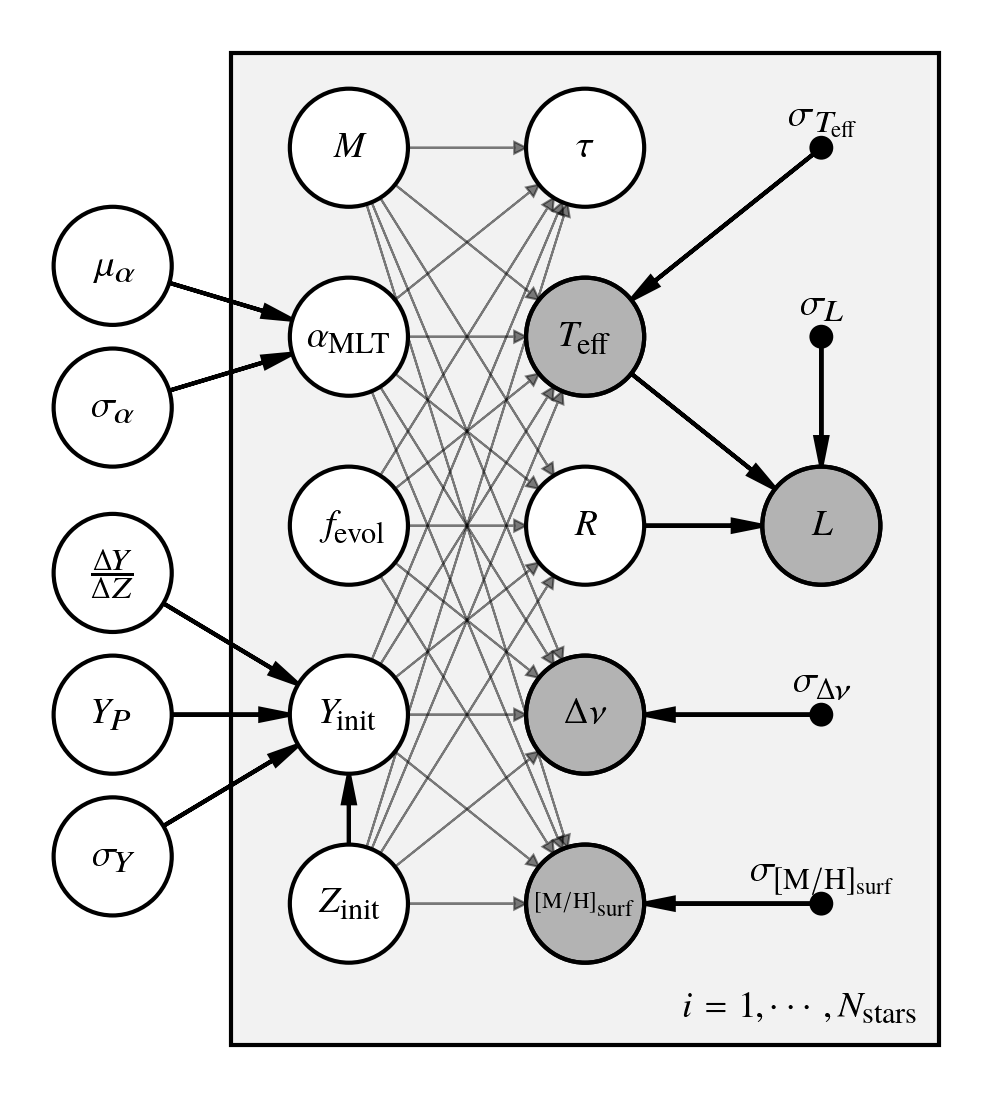
\includegraphics{figures/partial_pool_pgm.png}
    \caption[A probabilistic graphical model of the partially-pooled hierarchical model.]{A probabilistic graphical model (PGM) of the partially-pooled (PP) hierarchical model. Nodes outside the grey rectangle represent the hyperparameters in the model. Nodes inside the grey rectangle represent individual stellar parameters. Dark grey nodes represent observables which each have their respective observational uncertainties given by the solid black nodes. The direction of the arrows represent the dependencies in the generative model. \emph{This diagram was made using the \textsc{Python} package \texttt{daft} \citep{Foreman-Mackey.Hogg.ea2021}.}}
    \label{fig:pgm}
\end{figure}

It follows that the posterior PDF for a population of $N_\mathrm{stars}$ stars for the NP model is, 
%
\begin{equation}
    p(\boldsymbol{\Theta} | \boldsymbol{D}) = \prod_{i=1}^{N_{\mathrm{stars}}} p(\boldsymbol{\theta}_i | \boldsymbol{d}_i),   
\end{equation}
%
where $\boldsymbol{\Theta}$ is the matrix of model parameters and $\boldsymbol{D}$ is the matrix of observables. A probabilistic graphical model (PGM) of the NP model can be seen inside the grey box of Fig. \ref{fig:pgm}, without the arrow connecting $Z_\mathrm{init}$ to $Y_\mathrm{init}$. We ignore the nodes outside the box because these correspond to the PP model described next.

\subsubsection{Partial-Pooled (PP) Model}\label{sec:pp}

%%%%%%%%%%%%%%%%%%%%%%%%%%%%%%%%%%%%%%%%%%%%%%%%%%

%%%%%%%%%%%%% PARTIALLY POOLED MODEL %%%%%%%%%%%%%

Sharing, or pooling parameters between stars in a population can improve the uncertainties on stellar fundamentals by encoding our prior knowledge of their distribution in a population. We constructed a hierarchical model, which builds upon the NP model by introducing population-level \emph{hyperparameters}. Specifically, we chose to describe initial helium and $\mlt$ by partially-pooling them.

We constructed the PP model such that each of the initial helium, $\boldsymbol{Y}_\mathrm{init}$ and MLT parameter, $\boldsymbol{\alpha}_\mathrm{MLT}$ are drawn from a common distribution characterised by the set of hyperparameters, $\boldsymbol{\phi}$. Thus, Bayes' theorem becomes,
%
\begin{equation}
    p(\boldsymbol{\phi}, \boldsymbol{\Theta} | \boldsymbol{D}) \propto p(\boldsymbol{\phi}) \, p(\boldsymbol{Y}_\mathrm{init}, \boldsymbol{\alpha}_\mathrm{MLT} | \boldsymbol{\phi}) \, p(\boldsymbol{f}_{\mathrm{evol}}, \boldsymbol{M}, \boldsymbol{Z}) \, p(\boldsymbol{D} | \boldsymbol{\Theta}),
    \label{eq:hbmbayes}
\end{equation}
%
where $\boldsymbol{\Theta}$ is the same as in the NP model, i.e. each object-level parameter, $\boldsymbol{\theta}_j = \{\theta_{j, i}\}_{i=1}^{N_\mathrm{stars}}$, and $\boldsymbol{\phi} = \{\Delta Y/\Delta Z, Y_P, \sigma_Y, \mu_\alpha, \sigma_\alpha\}$. The hyperparameters for $\boldsymbol{Y}_\mathrm{init}$ comprise the helium enrichment ratio (${\Delta Y}/{\Delta Z}$), primordial helium abundance fraction ($Y_P$), and the spread in helium ($\sigma_Y$). The remaining hyperparameters for $\boldsymbol{\alpha}_\mathrm{MLT}$ comprise the mean ($\mu_\alpha$) and spread, ($\sigma_\alpha$).

We assumed the initial helium and the mixing-length parameter are each drawn from a normal distribution characterised by a population mean and standard deviation. The probability of $\boldsymbol{Y}_\mathrm{init}$ and $\boldsymbol{\alpha}_\mathrm{MLT}$ given $\boldsymbol{\phi}$ is,
%
\begin{equation}
    p(\boldsymbol{Y}_\mathrm{init}, \boldsymbol{\alpha}_\mathrm{MLT} | \boldsymbol{\phi}) = p(\boldsymbol{Y}_\mathrm{init} | \boldsymbol{\mu}_Y, \sigma_Y) \, p(\boldsymbol{\alpha}_\mathrm{MLT} | \mu_\alpha, \sigma_\alpha),
    \label{eq:ppool}
\end{equation}
%
where $\boldsymbol{\mu}_Y$ and is the mean initial helium fraction as described by the linear helium enrichment law,
%
\begin{equation}
    \boldsymbol{\mu}_{Y} = Y_P + \frac{\Delta Y}{\Delta Z} \boldsymbol{Z}_{\mathrm{init}}.\label{eq:helium}
\end{equation}
%
Therefore, we may write the prior PDF of initial helium given its population-level hyperparameters as,
%
\begin{equation}
    p(\boldsymbol{Y}_{\mathrm{init}} | \boldsymbol{Z}_{\mathrm{init}}, {\Delta Y}/{\Delta Z}, Y_P, \sigma_Y) = \prod_{i=1}^{N_\mathrm{stars}} \mathcal{N}({Y}_{\mathrm{init}, i} | {\mu}_{Y, i}, \sigma_Y).
\end{equation}
%

Similarly, for the second component of Equation \ref{eq:ppool}, we chose to partially-pool $\mlt$. We assume that convection in stars of a similar mass, evolutionary stage and area of the HR diagram may be approximated using a similar value of $\mlt$, but the accuracy of the MLT may vary from star-to-star. Given the small range of our sample, any such variation will be absorbed by the spread parameter, $\sigma_\alpha$. Therefore, we decided to describe the prior on $\boldsymbol{\alpha}_\mathrm{MLT}$ as,
%
\begin{equation}
    p(\boldsymbol{\alpha}_{\mathrm{MLT}} | \mu_\alpha, \sigma_\alpha) = \prod_{i=1}^{N_\mathrm{stars}} \mathcal{N}({\alpha}_{\mathrm{MLT}, i} | \mu_\alpha, \sigma_\alpha).
\end{equation}
%

We gave all the hyperparameters weakly informative priors, except for $Y_P$ for which we adopt a recent measurement of the primordial helium abundance from big bang nucleosynthesis (BBN) as the mean \citep{Pitrou.Coc.ea2018}, with a standard deviation representative of the range of values in the literature \citep{Aver.Olive.ea2015, Peimbert.Peimbert.ea2016, Cooke.Fumagalli2018}. Hence, we assumed priors on the hyperparameters as follows,
%
\begin{align*}
    {\Delta Y}/{\Delta Z} &\sim 4.0\cdot\mathcal{B}(1.2, 1.2),\\
    Y_P &\sim \mathcal{N}(0.247, 0.001),\\
    \sigma_Y &\sim \ln\mathcal{N}(0.01, 1.0),\\
    \mu_\alpha &\sim 1.5 + \mathcal{B}(1.2, 1.2),\\
    \sigma_\alpha &\sim \ln\mathcal{N}(0.1, 1.0),
\end{align*}
%
where, $x \sim \ln\mathcal{N}(m, \sigma)$ represents a random variable drawn from the log-normal distribution,
%
\begin{equation}
    \ln\mathcal{N}(x | m, \sigma)=  \frac{1}{x \sigma \sqrt{2 \pi}} \exp \left[ - \frac{\ln (x / m)^{2}}{2 \sigma^{2}}\right].
\end{equation}
%

We produced a PGM for the model, depicted in Fig. \ref{fig:pgm}. The hyperparameters are shown outside the grey box containing the individual stellar parameters to represent the hierarchical aspect of the model.

\subsubsection{Max-Pooled (MP) Model}\label{sec:mp}

%%%%%%%%%%%%%%%%%%%%%%%%%%%%%%%%%%%%%%%%%%%%%%%%%%

%%%%%%%%%%%%%%%% MAX-POOLED MODEL %%%%%%%%%%%%%%%%

We built another hierarchical model similar to the PP model except that $\mlt$ is max-pooled (MP). In this model, we assumed that $\mlt$ must be the same value for every star in the sample, but still allowed it to freely vary on a population-level. Thus, the hyperparameters are now, $\boldsymbol{\phi} = \{\Delta Y/\Delta Z, Y_P, \sigma_Y, \mlt\}$. The posterior distribution of the model takes the same form as in Equation \ref{eq:hbmbayes} except that the MLT parameter for the $i$-th star is,
%
\begin{equation}
    \alpha_{\mathrm{MLT}, i} = \mlt,
\end{equation}
%
where,
\begin{equation}
    \mlt \sim 1.5 + \mathcal{B}(1.2, 1.2),
\end{equation}
%
chosen such that $\mlt$ is confined to the boundaries of the grid of stellar models ($1.5 < \mlt < 2.5$).

\subsection{The Sun as a Star}\label{sec:sun}

Pooling parameters in an HBM allows us to use the Sun as a calibrator uniquely. Rather than calibrating our model physics to the Sun and then assuming the calibrated parameters across our sample, we can include the Sun as a part of the same population as our sample of stars. If we assume $Y_\mathrm{init}$ and $\mlt$ for the Sun are a part of the same prior distribution as for the rest of the sample, then we can simply add solar observables to our model inputs.

For both the PP and MP models, we iterated with and without data for the Sun included in the population, referred to as PPS and MPS respectively. We adopted the solar data in Table \ref{tab:sun} with uncertainties conservatively limited to the accuracy of the ANN for $R$, $L$ and representative of variation in the literature for $\teff$. We also adopted $\dnu=\SI{135.1(2)}{\micro\hertz}$ with a central value from \citet{Huber.Bedding.ea2011} and a standard deviation representative of variations in measurements of the solar $\dnu$ \citep{Broomhall.Chaplin.ea2011}.

\begin{table}
    \centering
    \caption[Solar input data.]{Solar input data. The references correspond to the central values and the uncertainties are chosen to either be representative of the ANN accuracy or the spread of values in the literature (see text for details).}
    \label{tab:sun}
    \begin{tabular}{lcc}
\toprule
                            Input &            Value &                         Reference \\
\midrule
                    $M\,(\si{\solarmass})$ &  $1.000\pm0.001$ &                               --- \\
                 $\tau\,(\si{\giga\year})$ &      $4.6\pm0.1$ &  \citet{Connelly.Bizzarro.ea2012} \\
                   $\teff\,(\si{\kelvin})$ &      $5777\pm20$ &     \citet{Scott.Grevesse.ea2015} \\
                  $R\,(\si{\solarradius})$ &  $1.000\pm0.001$ &                               --- \\
              $L\,(\si{\solarluminosity})$ &    $1.00\pm0.01$ &                               --- \\
               $\dnu\,(\si{\micro\hertz})$ &    $135.1\pm0.2$ &      \citet{Huber.Bedding.ea2011} \\
 $\metallicity_\mathrm{surf}\,(\si{\dex})$ &    $0.00\pm0.01$ &   \citet{Asplund.Grevesse.ea2009} \\
\bottomrule
\end{tabular}

\end{table}

\subsection{Sampling}\label{sec:sampling}

We obtained results for each of the models described above by sampling their posterior distributions using a Markov chain Monte Carlo (MCMC) algorithm. In particular, we used the NUTS algorithm implemented in \textsc{TensorFlow Probability} \citep[\textsc{TFP};][]{Abadi.Barham.ea2016, Dillon.Langmore.ea2017}\footnote{We interacted with \textsc{TFP} using the now deprecated \textsc{PyMC4} package, developed as a successor to \textsc{PyMC3} \citep{Salvatier.Wiecki.ea2016}.}. For each model, we produced \num{20000} samples split across \num{10} MCMC chains and computed summary statistics for the marginalised posteriors of each parameter in the model. We removed stars with problems during tuning using the Gelman-Rubin diagnostic \citep[$\hat{r}$;][]{Gelman.Rubin1992}. We used results from each model once $\hat{r} < 1.04$ for all parameters, indicating good model convergence.

Initially, we created a random synthetic population of stars using \textsc{MESA} to test the ability of the method to recover stellar properties according to our choice of model physics and population priors. We tested the NP, PP, and MP models. Since our sample was fictitious, it would not have been appropriate to include real solar data. We summarise the results for the synthetic stellar parameters and hyperparameters in Appendix \ref{sec:test-stars}. We found that the models were able to recover the true synthetic properties accurately, with increased precision when pooling parameters.

Once we had tested the method on synthetic stars, we obtained results for the sample of 81 dwarfs and subgiants described in Section \ref{sec:data}. Here, we included the PPS and MPS to test the effects of adding the Sun as a star in our population. For the purpose of comparison, we fit the hyperparameters of the PP model ($\Delta Y/\Delta Z, Y_P, \sigma_Y, \mu_\alpha, \sigma_\alpha$) to the results from the NP model.

Since our initial sample was chosen based on masses from \citetalias{Serenelli.Johnson.ea2017}, we expected some stars to lie outside (or near the boundary) of the observational parameter space provided by our grid of stellar models. We used an initial run of the NP model to catch and remove these stars. During the initial run, we dropped 16 of the 81 stars from the sample. Of the removed stars, we found the posteriors in $M$ for 6 skewed towards the prior upper mass limit of \SI{1.2}{\solarmass}. The remaining 10 removed stars suffered poor convergence during sampling ($\hat{r} >> 1.04$) which could be because of poor step-size tuning and sampling at the prior boundary.

Out of the remaining 65 stars with results from the NP model, 2 stars were dropped from the PP model. A consequence of partially pooling parameters is that a population spread, $\sigma$ allows for individual parameters to vary outside the prior range given to the population mean, $\mu$. In this case, individual stellar $\mlt$ was allowed to vary outside the range for which the ANN was valid if $\sigma_\alpha$ was large. The 2 removed stars happened to have high likelihoods outside the valid $\mlt$ range. We found that removing the same 2 stars from the other models made negligible difference to the results, so we leave a solution to this problem to future work. Naturally, we did not see the same issue in the MP model, so we proceeded with modelling the same 65 stars as with the NP model.

\section{Results}\label{sec:res}

%%%%%%%%%%%%%%%%%%%%%%%%%%%%%%%%%%%%%%%%%%%%%%%%%%

%%%%%%%%%%%%%%%%%%%% RESULTS %%%%%%%%%%%%%%%%%%%%%

In this section, we present the results for each of the NP, PP, and MP models with the sample of 81 APOKASC dwarfs and subgiants as inputs. We also present the results for the PPS and MPS models which include the Sun as a star in the population. Firstly, we show the reduction in age, mass and radius uncertainty with the addition of pooling in Section \ref{sec:param-results}. We then show the results for model hyperparameters in Section \ref{sec:hparam-results} where we infer the initial helium abundance and mixing-length parameter distribution in the sample.

\subsection{Stellar Parameter Results}\label{sec:param-results}

In Table \ref{tab:np}, we present results for the 65 APOKASC stars from the NP model. Running the NP model with synthetic stars resulted in unreliable uncertainties (see Appendix \ref{sec:test-stars}). This was because the boundary of the priors in $Y_\mathrm{init}$ and $\mlt$ truncated the posterior distribution leading to underestimated uncertainties and skewing their posterior means towards the centre of their priors. Therefore, we present the NP results only for comparison purposes, but we exclude them from further discussion. In Tables \ref{tab:pp} and \ref{tab:pps} we present the results for the 63 stars from the PP and PPS model respectively. In Tables \ref{tab:mp} and \ref{tab:mps} we also present results for the 65 stars from the MP and MPS models respectively. We note that for the MP models, there is no column for $\mlt$ because this parameter is the same across the population and hence is given in Section \ref{sec:hparam-results}.

\begin{landscape}
\begin{table*}
	\centering
	\caption[The median of the marginalised posterior samples for selected parameters output by the NP model.]{The median of the marginalised posterior samples for selected parameters output by the NP model, with their respective upper and lower 68 per cent credible intervals. The full table is available as supplementary material in the original article \citep{Lyttle.Davies.ea2021}.}
	\label{tab:np}
	\begin{tabular}{lcccccc}  %cccc}
\toprule
Name &                $f_\mathrm{evol}$ &           $M\,(\si{\solarmass})$ &                           $\mlt$ &                $Y_\mathrm{init}$ &                   $Z_\mathrm{init}$ &     $\tau\,(\si{\giga\year})$ \\  %&       $\teff\,(\si{\kelvin})$ &         $R\,(\si{\solarradius})$ &     $\dnu\,(\si{\micro\hertz})$ & $\metallicity_\mathrm{surf}\,(\si{\dex})$ \\
\midrule
  KIC10079226 &  $0.44\substack{+0.16 \\ -0.20}$ &  $1.14\substack{+0.04 \\ -0.04}$ &  $2.07\substack{+0.26 \\ -0.30}$ &  $0.28\substack{+0.02 \\ -0.02}$ &  $0.021\substack{+0.003 \\ -0.003}$ &  $2.5\substack{+1.2 \\ -1.3}$ \\  %&  $5990\substack{+51 \\ -52}$ &  $1.16\substack{+0.01 \\ -0.02}$ &  $116.0\substack{+0.7 \\ -0.7}$ &           $0.16\substack{+0.07 \\ -0.07}$ \\
  KIC10215584 &  $0.50\substack{+0.21 \\ -0.21}$ &  $1.13\substack{+0.04 \\ -0.05}$ &  $1.92\substack{+0.33 \\ -0.26}$ &  $0.27\substack{+0.02 \\ -0.02}$ &  $0.018\substack{+0.002 \\ -0.002}$ &  $2.9\substack{+1.6 \\ -1.3}$ \\  %&  $5949\substack{+64 \\ -65}$ &  $1.18\substack{+0.02 \\ -0.02}$ &  $112.5\substack{+2.6 \\ -2.6}$ &           $0.08\substack{+0.06 \\ -0.06}$ \\
  KIC10319352 &  $1.51\substack{+0.15 \\ -0.28}$ &  $1.09\substack{+0.05 \\ -0.05}$ &  $1.87\substack{+0.33 \\ -0.23}$ &  $0.28\substack{+0.03 \\ -0.02}$ &  $0.028\substack{+0.004 \\ -0.003}$ &  $9.6\substack{+1.7 \\ -1.5}$ \\  %&  $5507\substack{+57 \\ -56}$ &  $1.49\substack{+0.03 \\ -0.03}$ &   $78.6\substack{+1.6 \\ -1.6}$ &           $0.28\substack{+0.06 \\ -0.06}$ \\
  KIC10322381 &  $0.98\substack{+0.23 \\ -0.28}$ &  $1.07\substack{+0.07 \\ -0.07}$ &  $2.04\substack{+0.29 \\ -0.31}$ &  $0.28\substack{+0.02 \\ -0.02}$ &  $0.010\substack{+0.002 \\ -0.002}$ &  $4.7\substack{+1.5 \\ -1.7}$ \\  %&  $6132\substack{+94 \\ -94}$ &  $1.39\substack{+0.05 \\ -0.04}$ &   $85.6\substack{+4.9 \\ -4.6}$ &          $-0.30\substack{+0.07 \\ -0.08}$ \\
  KIC10732098 &  $1.60\substack{+0.14 \\ -0.19}$ &  $1.12\substack{+0.04 \\ -0.05}$ &  $1.86\substack{+0.33 \\ -0.23}$ &  $0.28\substack{+0.02 \\ -0.02}$ &  $0.017\substack{+0.002 \\ -0.002}$ &  $6.7\substack{+0.8 \\ -0.8}$ \\  %&  $5720\substack{+67 \\ -66}$ &  $1.77\substack{+0.04 \\ -0.04}$ &   $62.1\substack{+1.8 \\ -1.7}$ &           $0.06\substack{+0.07 \\ -0.07}$ \\
\bottomrule
\end{tabular}

\end{table*}

\begin{table*}
	\centering
	\caption{The same as Table \ref{tab:np}, but for the PP model.}
	\label{tab:pp}
	\begin{tabular}{lcccccccccc}
\toprule
Name &                $f_\mathrm{evol}$ &           $M\,(\si{\solarmass})$ &                           $\mlt$ &                $Y_\mathrm{init}$ &                   $Z_\mathrm{init}$ &     $\tau\,(\si{\giga\year})$ &      $\teff\,(\si{\kelvin})$ &         $R\,(\si{\solarradius})$ &     $\dnu\,(\si{\micro\hertz})$ & $\metallicity_\mathrm{surf}\,(\si{\dex})$ \\
\midrule
  KIC10079226 &  $0.22\substack{+0.10 \\ -0.09}$ &  $1.16\substack{+0.02 \\ -0.03}$ &  $1.75\substack{+0.11 \\ -0.09}$ &  $0.28\substack{+0.01 \\ -0.01}$ &  $0.020\substack{+0.003 \\ -0.002}$ &  $1.2\substack{+0.6 \\ -0.5}$ &  $5962\substack{+44 \\ -42}$ &  $1.17\substack{+0.01 \\ -0.01}$ &  $115.9\substack{+0.7 \\ -0.7}$ &           $0.15\substack{+0.07 \\ -0.07}$ \\
  KIC10215584 &  $0.37\substack{+0.15 \\ -0.13}$ &  $1.14\substack{+0.03 \\ -0.03}$ &  $1.74\substack{+0.10 \\ -0.09}$ &  $0.27\substack{+0.01 \\ -0.01}$ &  $0.018\substack{+0.002 \\ -0.002}$ &  $2.1\substack{+1.0 \\ -0.8}$ &  $5941\substack{+57 \\ -56}$ &  $1.18\substack{+0.02 \\ -0.02}$ &  $112.5\substack{+2.6 \\ -2.7}$ &           $0.07\substack{+0.07 \\ -0.07}$ \\
  KIC10319352 &  $1.41\substack{+0.11 \\ -0.27}$ &  $1.08\substack{+0.03 \\ -0.03}$ &  $1.73\substack{+0.10 \\ -0.09}$ &  $0.29\substack{+0.02 \\ -0.01}$ &  $0.028\substack{+0.004 \\ -0.004}$ &  $8.6\substack{+1.1 \\ -1.0}$ &  $5512\substack{+45 \\ -46}$ &  $1.49\substack{+0.02 \\ -0.02}$ &   $78.6\substack{+1.6 \\ -1.6}$ &           $0.28\substack{+0.06 \\ -0.07}$ \\
  KIC10322381 &  $0.78\substack{+0.23 \\ -0.19}$ &  $1.14\substack{+0.03 \\ -0.06}$ &  $1.75\substack{+0.10 \\ -0.09}$ &  $0.26\substack{+0.01 \\ -0.01}$ &  $0.011\substack{+0.002 \\ -0.002}$ &  $3.6\substack{+1.7 \\ -1.1}$ &  $6081\substack{+95 \\ -92}$ &  $1.41\substack{+0.05 \\ -0.05}$ &   $86.2\substack{+4.8 \\ -5.2}$ &          $-0.31\substack{+0.07 \\ -0.07}$ \\
  KIC10732098 &  $1.50\substack{+0.13 \\ -0.14}$ &  $1.14\substack{+0.03 \\ -0.04}$ &  $1.74\substack{+0.10 \\ -0.09}$ &  $0.28\substack{+0.01 \\ -0.01}$ &  $0.018\substack{+0.002 \\ -0.002}$ &  $6.4\substack{+0.6 \\ -0.6}$ &  $5701\substack{+59 \\ -58}$ &  $1.78\substack{+0.03 \\ -0.03}$ &   $62.2\substack{+1.7 \\ -1.7}$ &           $0.06\substack{+0.06 \\ -0.06}$ \\
\bottomrule
\end{tabular}

\end{table*}

\begin{table*}
	\centering
	\caption{The same as Table \ref{tab:np}, but for the PPS model.}
	\label{tab:pps}
	\begin{tabular}{lccccccccccc}
\toprule
Name &                $f_\mathrm{evol}$ &           $M\,(\si{\solarmass})$ &                           $\mlt$ &                $Y_\mathrm{init}$ &                   $Z_\mathrm{init}$ &     $\tau\,(\si{\giga\year})$ &      $\teff\,(\si{\kelvin})$ &         $R\,(\si{\solarradius})$ &     $\dnu\,(\si{\micro\hertz})$ & $\metallicity_\mathrm{surf}\,(\si{\dex})$ \\
\midrule
  KIC10079226 &  $0.35\substack{+0.11 \\ -0.12}$ &  $1.17\substack{+0.02 \\ -0.03}$ &  $1.95\substack{+0.14 \\ -0.15}$ &  $0.27\substack{+0.01 \\ -0.01}$ &  $0.020\substack{+0.003 \\ -0.002}$ &  $2.1\substack{+0.8 \\ -0.8}$ &  $5962\substack{+44 \\ -43}$ &  $1.17\substack{+0.01 \\ -0.01}$ &  $116.0\substack{+0.7 \\ -0.7}$ &           $0.15\substack{+0.06 \\ -0.07}$ \\
  KIC10215584 &  $0.47\substack{+0.16 \\ -0.16}$ &  $1.14\substack{+0.03 \\ -0.03}$ &  $1.90\substack{+0.15 \\ -0.17}$ &  $0.27\substack{+0.01 \\ -0.01}$ &  $0.018\substack{+0.002 \\ -0.002}$ &  $2.7\substack{+1.2 \\ -1.1}$ &  $5943\substack{+56 \\ -58}$ &  $1.18\substack{+0.02 \\ -0.02}$ &  $112.6\substack{+2.6 \\ -2.6}$ &           $0.07\substack{+0.06 \\ -0.07}$ \\
  KIC10319352 &  $1.51\substack{+0.10 \\ -0.22}$ &  $1.09\substack{+0.03 \\ -0.03}$ &  $1.88\substack{+0.16 \\ -0.16}$ &  $0.28\substack{+0.01 \\ -0.01}$ &  $0.028\substack{+0.004 \\ -0.004}$ &  $9.6\substack{+1.1 \\ -1.2}$ &  $5507\substack{+47 \\ -48}$ &  $1.49\substack{+0.02 \\ -0.02}$ &   $78.6\substack{+1.6 \\ -1.6}$ &           $0.28\substack{+0.06 \\ -0.06}$ \\
  KIC10322381 &  $0.89\substack{+0.21 \\ -0.22}$ &  $1.12\substack{+0.05 \\ -0.06}$ &  $1.93\substack{+0.15 \\ -0.16}$ &  $0.26\substack{+0.01 \\ -0.01}$ &  $0.010\substack{+0.002 \\ -0.002}$ &  $4.3\substack{+1.7 \\ -1.2}$ &  $6093\substack{+92 \\ -89}$ &  $1.41\substack{+0.04 \\ -0.04}$ &   $86.1\substack{+5.0 \\ -4.9}$ &          $-0.31\substack{+0.07 \\ -0.08}$ \\
  KIC10732098 &  $1.60\substack{+0.11 \\ -0.14}$ &  $1.14\substack{+0.03 \\ -0.04}$ &  $1.90\substack{+0.15 \\ -0.17}$ &  $0.27\substack{+0.01 \\ -0.01}$ &  $0.017\substack{+0.002 \\ -0.002}$ &  $6.9\substack{+0.6 \\ -0.6}$ &  $5704\substack{+62 \\ -61}$ &  $1.78\substack{+0.04 \\ -0.03}$ &   $62.2\substack{+1.8 \\ -1.7}$ &           $0.06\substack{+0.06 \\ -0.06}$ \\
\bottomrule
\end{tabular}

\end{table*}

\begin{table*}
	\centering
	\caption{The same as Table \ref{tab:np}, but for the MP model.}
	\label{tab:mp}
	\begin{tabular}{lccccccccc}
\toprule
Name &                $f_\mathrm{evol}$ &           $M\,(\si{\solarmass})$ &                $Y_\mathrm{init}$ &                   $Z_\mathrm{init}$ &     $\tau\,(\si{\giga\year})$ &      $\teff\,(\si{\kelvin})$ &         $R\,(\si{\solarradius})$ &     $\dnu\,(\si{\micro\hertz})$ & $\metallicity_\mathrm{surf}\,(\si{\dex})$ \\
\midrule
  KIC10079226 &  $0.20\substack{+0.08 \\ -0.08}$ &  $1.17\substack{+0.02 \\ -0.03}$ &  $0.28\substack{+0.01 \\ -0.01}$ &  $0.019\substack{+0.003 \\ -0.002}$ &  $1.1\substack{+0.5 \\ -0.4}$ &  $5961\substack{+42 \\ -41}$ &  $1.17\substack{+0.01 \\ -0.01}$ &  $115.9\substack{+0.7 \\ -0.7}$ &           $0.15\substack{+0.06 \\ -0.07}$ \\
  KIC10215584 &  $0.36\substack{+0.14 \\ -0.13}$ &  $1.14\substack{+0.03 \\ -0.03}$ &  $0.27\substack{+0.01 \\ -0.01}$ &  $0.018\substack{+0.002 \\ -0.002}$ &  $2.0\substack{+0.9 \\ -0.8}$ &  $5941\substack{+57 \\ -57}$ &  $1.18\substack{+0.02 \\ -0.02}$ &  $112.5\substack{+2.6 \\ -2.7}$ &           $0.07\substack{+0.06 \\ -0.07}$ \\
  KIC10319352 &  $1.41\substack{+0.10 \\ -0.25}$ &  $1.08\substack{+0.03 \\ -0.03}$ &  $0.29\substack{+0.02 \\ -0.01}$ &  $0.028\substack{+0.004 \\ -0.004}$ &  $8.6\substack{+1.0 \\ -0.9}$ &  $5512\substack{+44 \\ -45}$ &  $1.49\substack{+0.02 \\ -0.02}$ &   $78.6\substack{+1.7 \\ -1.6}$ &           $0.28\substack{+0.06 \\ -0.07}$ \\
  KIC10322381 &  $0.77\substack{+0.23 \\ -0.19}$ &  $1.14\substack{+0.04 \\ -0.06}$ &  $0.27\substack{+0.01 \\ -0.01}$ &  $0.011\substack{+0.002 \\ -0.002}$ &  $3.5\substack{+1.6 \\ -1.0}$ &  $6076\substack{+96 \\ -91}$ &  $1.41\substack{+0.05 \\ -0.05}$ &   $86.1\substack{+4.7 \\ -5.3}$ &          $-0.32\substack{+0.07 \\ -0.07}$ \\
  KIC10732098 &  $1.50\substack{+0.13 \\ -0.13}$ &  $1.14\substack{+0.03 \\ -0.04}$ &  $0.28\substack{+0.01 \\ -0.01}$ &  $0.018\substack{+0.002 \\ -0.002}$ &  $6.4\substack{+0.6 \\ -0.6}$ &  $5702\substack{+56 \\ -58}$ &  $1.78\substack{+0.03 \\ -0.03}$ &   $62.2\substack{+1.7 \\ -1.7}$ &           $0.06\substack{+0.06 \\ -0.06}$ \\
\bottomrule
\end{tabular}

\end{table*}

\begin{table*}
	\centering
	\caption{The same as Table \ref{tab:np}, but for the MPS model.}
	\label{tab:mps}
	\begin{tabular}{lccccccccc}
\toprule
Name &                $f_\mathrm{evol}$ &           $M\,(\si{\solarmass})$ &                $Y_\mathrm{init}$ &                   $Z_\mathrm{init}$ &      $\tau\,(\si{\giga\year})$ &      $\teff\,(\si{\kelvin})$ &         $R\,(\si{\solarradius})$ &     $\dnu\,(\si{\micro\hertz})$ & $\metallicity_\mathrm{surf}\,(\si{\dex})$ \\
\midrule
  KIC10079226 &  $0.44\substack{+0.07 \\ -0.06}$ &  $1.16\substack{+0.02 \\ -0.03}$ &  $0.26\substack{+0.01 \\ -0.01}$ &  $0.021\substack{+0.003 \\ -0.002}$ &   $2.7\substack{+0.5 \\ -0.4}$ &  $5965\substack{+40 \\ -40}$ &  $1.17\substack{+0.01 \\ -0.01}$ &  $116.0\substack{+0.7 \\ -0.7}$ &           $0.15\substack{+0.06 \\ -0.06}$ \\
  KIC10215584 &  $0.59\substack{+0.11 \\ -0.13}$ &  $1.13\substack{+0.03 \\ -0.03}$ &  $0.26\substack{+0.01 \\ -0.01}$ &  $0.018\substack{+0.002 \\ -0.002}$ &   $3.6\substack{+0.9 \\ -0.9}$ &  $5952\substack{+55 \\ -56}$ &  $1.18\substack{+0.02 \\ -0.02}$ &  $112.7\substack{+2.7 \\ -2.7}$ &           $0.08\substack{+0.06 \\ -0.07}$ \\
  KIC10319352 &  $1.61\substack{+0.04 \\ -0.06}$ &  $1.08\substack{+0.03 \\ -0.03}$ &  $0.27\substack{+0.01 \\ -0.01}$ &  $0.028\substack{+0.004 \\ -0.003}$ &  $10.8\substack{+0.7 \\ -0.8}$ &  $5516\substack{+46 \\ -47}$ &  $1.49\substack{+0.02 \\ -0.02}$ &   $78.6\substack{+1.7 \\ -1.6}$ &           $0.28\substack{+0.07 \\ -0.06}$ \\
  KIC10322381 &  $0.98\substack{+0.19 \\ -0.20}$ &  $1.10\substack{+0.06 \\ -0.05}$ &  $0.26\substack{+0.01 \\ -0.01}$ &  $0.010\substack{+0.002 \\ -0.001}$ &   $5.1\substack{+1.3 \\ -1.5}$ &  $6106\substack{+94 \\ -80}$ &  $1.40\substack{+0.04 \\ -0.04}$ &   $85.8\substack{+5.6 \\ -4.3}$ &          $-0.30\substack{+0.08 \\ -0.08}$ \\
  KIC10732098 &  $1.69\substack{+0.06 \\ -0.09}$ &  $1.14\substack{+0.03 \\ -0.04}$ &  $0.26\substack{+0.01 \\ -0.01}$ &  $0.017\substack{+0.002 \\ -0.002}$ &   $7.4\substack{+0.5 \\ -0.5}$ &  $5715\substack{+61 \\ -61}$ &  $1.77\substack{+0.04 \\ -0.03}$ &   $62.3\substack{+1.8 \\ -1.8}$ &           $0.07\substack{+0.06 \\ -0.07}$ \\
\bottomrule
\end{tabular}

\end{table*}
\end{landscape}

\subsection{Population Parameter Results}\label{sec:hparam-results}

We obtained values for the hyperparameters for each of the models and present them in Table \ref{tab:hparam_results} along with their upper and lower 68 per cent credible regions. We omit the results for $Y_P$ because its posterior is the same as the prior, $Y_P=0.247\pm0.001$ for all the models. We fit the same hyperparameters from the PP model to the NP model results for $Y_\mathrm{init}$, $Z_\mathrm{init}$, and $\mlt$ for the purpose of comparison. However, the NP model results suffer from boundary effects which makes the resulting fit unreliable, pushing the population mean to the centre of the priors and underestimating the uncertainties. We leave the NP results here only for completeness.

\begin{table*}
	\centering
	\caption{Hyperparameter results for each model with the omission of $Y_P$.}
	\label{tab:hparam_results}
	\begin{tabular}{lccccc}
\toprule
Model &              $\Delta Y/\Delta Z$ &                             $\sigma_Y$ &                        $\mu_\alpha$ &                     $\sigma_\alpha$ &               $\alpha_\mathrm{mlt}$ \\
\midrule
            NP &  $1.69\substack{+0.21 \\ -0.21}$ &  $0.0074\substack{+0.0026 \\ -0.0022}$ &  $1.954\substack{+0.040 \\ -0.041}$ &  $0.065\substack{+0.030 \\ -0.024}$ &                                 --- \\
            PP &  $1.60\substack{+0.45 \\ -0.42}$ &  $0.0051\substack{+0.0045 \\ -0.0027}$ &  $1.742\substack{+0.081 \\ -0.070}$ &  $0.056\substack{+0.051 \\ -0.030}$ &                                 --- \\
           PPS &  $1.05\substack{+0.28 \\ -0.25}$ &  $0.0045\substack{+0.0038 \\ -0.0023}$ &  $1.900\substack{+0.095 \\ -0.088}$ &  $0.133\substack{+0.057 \\ -0.047}$ &                                 --- \\
            MP &  $1.60\substack{+0.45 \\ -0.42}$ &  $0.0051\substack{+0.0044 \\ -0.0027}$ &                                 --- &                                 --- &  $1.728\substack{+0.077 \\ -0.066}$ \\
           MPS &  $0.76\substack{+0.24 \\ -0.27}$ &  $0.0049\substack{+0.0039 \\ -0.0025}$ &                                 --- &                                 --- &  $2.088\substack{+0.031 \\ -0.029}$ \\
\bottomrule
\end{tabular}

\end{table*}

\begin{figure}
    \centering
    \begin{subfigure}[b]{.66\linewidth}
        \centering
        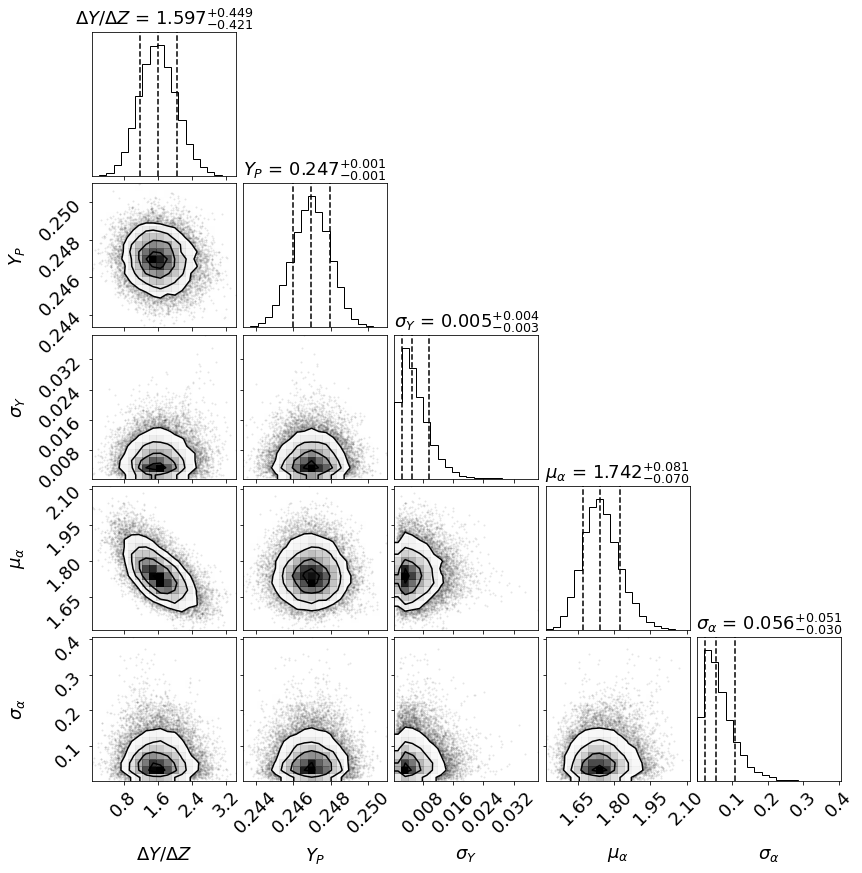
\includegraphics[width=\textwidth]{figures/corner_plot_pp.png}
    \end{subfigure}

    \begin{subfigure}[b]{.66\linewidth}
        \centering
        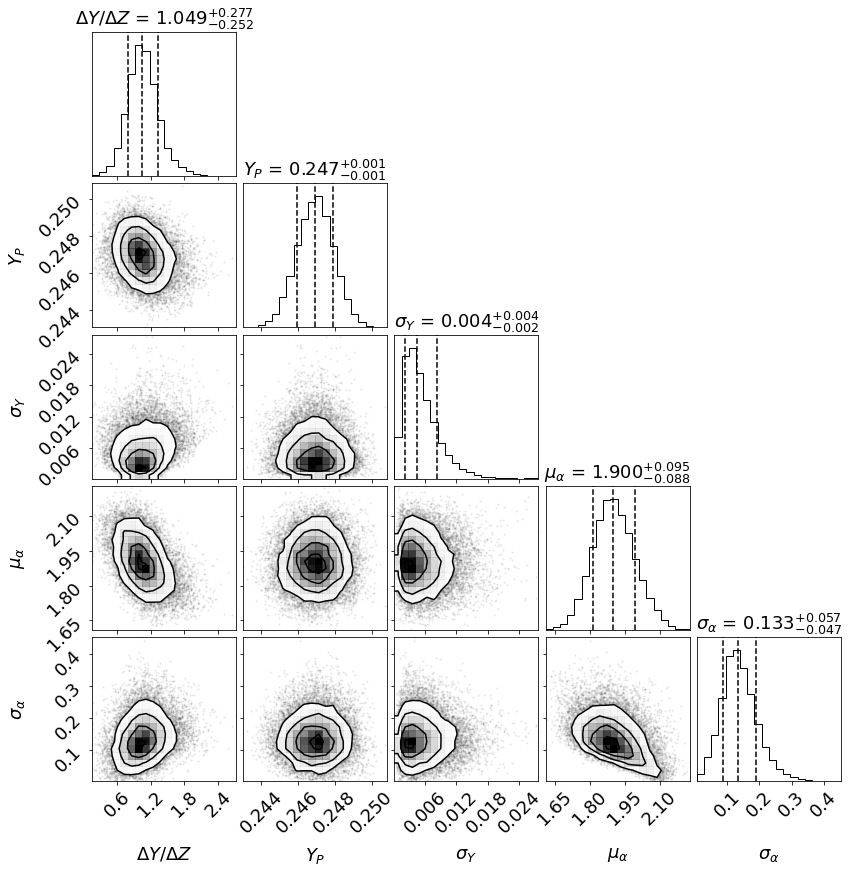
\includegraphics[width=\textwidth]{figures/corner_plot_pps.png}
    \end{subfigure}
    \caption[Corner plots showing the joint and marginalised sampled posterior distributions for the PP and PPS hyperparameters.]{Corner plots showing the joint and marginalised sampled posterior distributions for the hyperparameters for the PP (top) and PPS (bottom) models. The vertical dashed lines give the 16th, 50th and 84th percentiles.}
    \label{fig:corners-pp}
\end{figure} 

\begin{figure}
    \centering
    \begin{subfigure}[b]{.66\linewidth}
        \centering
        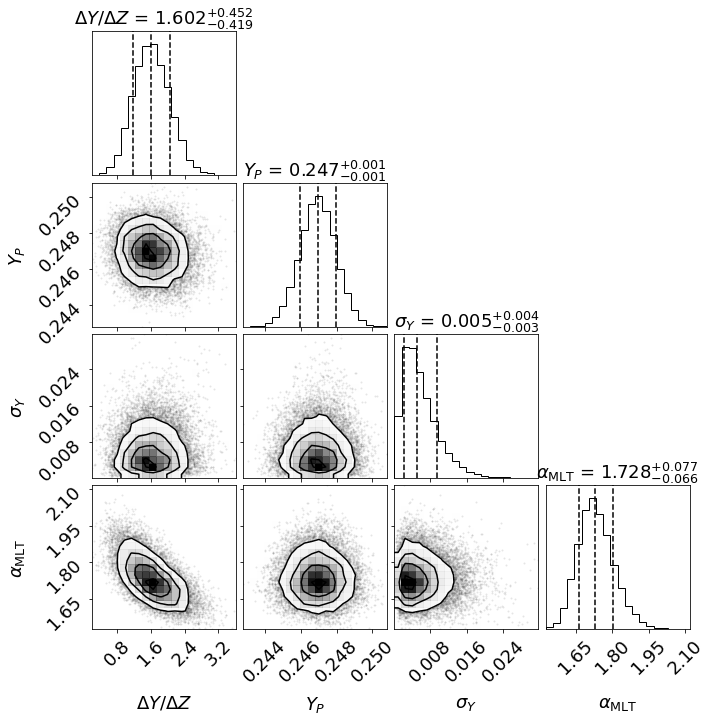
\includegraphics[width=\textwidth]{figures/corner_plot_mp.png}
    \end{subfigure}

    \begin{subfigure}[b]{.66\linewidth}
        \centering
        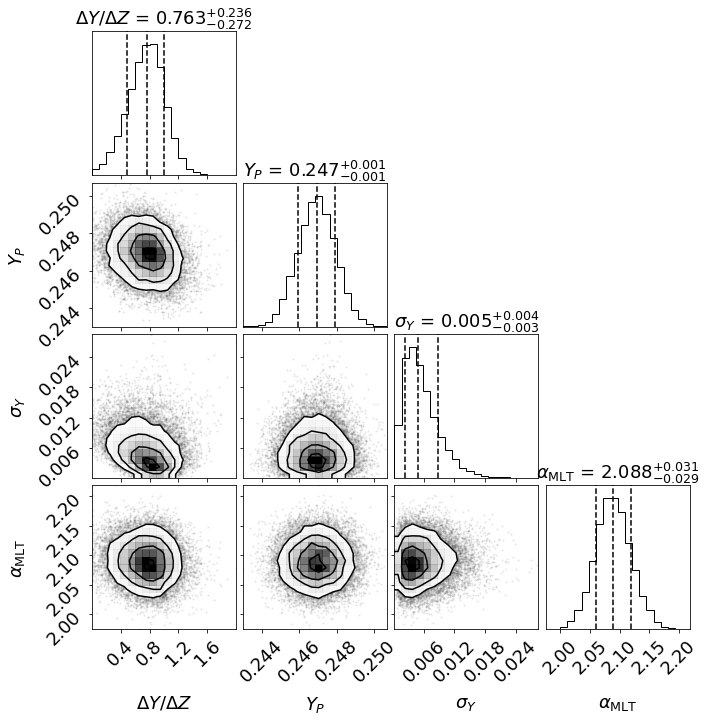
\includegraphics[width=\textwidth]{figures/corner_plot_mps.png}
    \end{subfigure}
    \caption{The same as Fig. \ref{fig:corners-pp} but for the MP (top) and MPS (bottom) models.}
    \label{fig:corners-mp}
\end{figure} 

Fig. \ref{fig:corners-pp} shows the joint and marginal distributions (corner plot) output by the PP and PPS model. We see an anti-correlation between $\Delta Y / \Delta Z$ and $\mu_\alpha$, expected due to the degeneracy between the two parameters in the stellar evolutionary models. In Fig. \ref{fig:corners-mp}, we also show the corner plot for the MP and MPS model output. Similarly, we see an anti-correlation between $\Delta Y / \Delta Z$ and $\mlt$.

\begin{figure}[tb]
    \centering
    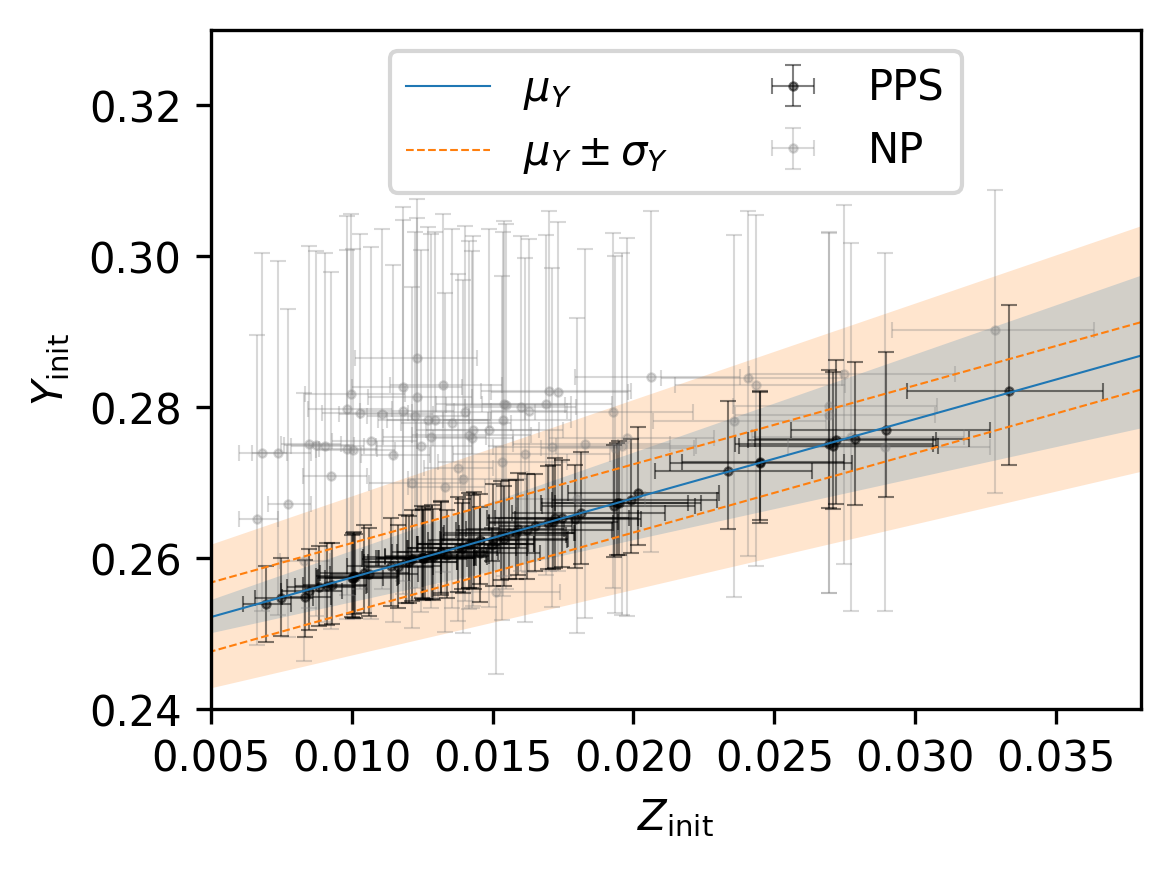
\includegraphics{figures/zi_yi_results_plot.png}
    \caption[The results for initial helium fraction against initial heavy-element fraction for each star from the PPS model.]{The results for initial helium fraction ($Y_\mathrm{init}$) against initial heavy-element fraction ($Z_\mathrm{init}$) for each star from the PPS model are shown by the black markers. The mean helium enrichment, $\mu_Y = Y_P + (\Delta Y / \Delta Z) Z_\mathrm{init}$ with its 68 per cent credible interval are shown in blue by a solid line and shaded region respectively. The population spread, $\mu_Y \pm \sigma_Y$ and its 68 per cent credible interval are shown in orange by a dashed line and shaded region respectively. The individual results from the NP model are shown by the light grey markers.}
    \label{fig:helium}
\end{figure}

We present the helium enrichment relation resulting from the PPS model in Fig. \ref{fig:helium}. In this figure, we plot the individual results for $Y_\mathrm{init}$ and $Z_\mathrm{init}$ for each of the stars from the NP and PPS models. This is an example of shrinkage in the HBM; the estimates for individual stellar parameters move towards the mean of the population when they are pooled.

\section{Discussion}\label{sec:dis}

%%%%%%%%%%%%%%%%%%%%%%%%%%%%%%%%%%%%%%%%%%%%%%%%%%

%%%%%%%%%%%%%%%%%%%% DISCUSSION %%%%%%%%%%%%%%%%%%

So far, we have shown that we can add parameters to stellar models without sacrificing statistical uncertainties through the application of an HBM. We freed the $Y_\mathrm{init}$ and $\mlt$ using pooling to encode our prior knowledge of their distribution in the population. We also tested the impact of including the Sun as a star in our population. We first discuss the impact of pooling and our choice of population priors for $Y_\mathrm{init}$ and $\mlt$ in Section \ref{sec:helium} and \ref{sec:mlt}. To assess the accuracy of our model with respect to the literature, we compare our results to those of \citetalias{Serenelli.Johnson.ea2017} in Section \ref{sec:comp}. We found good agreement between this work and their results, despite some differences in observables and stellar model physics which we discuss further. Then, we discuss sources of systematic uncertainties in Section \ref{sec:sys}. Although we have accounted for uncertainties in \ref{sec:helium} and \ref{sec:mlt} in our model, there are still differences between stellar modelling codes and other model physics which should be considered. Finally, in Section \ref{sec:out}, we highlight a possible outlier in our dataset.

\subsection{Helium Enrichment}\label{sec:helium}

We found the value for the helium enrichment ratio, $\Delta Y / \Delta Z$ to be the same in both the PP and MP models, $\Delta Y / \Delta Z = 1.6\substack{+0.5\\-0.4}$. This is consistent with values of $\sim 1.4$ in the literature (when heavy element diffusion is included) albeit obtained through different methods: e.g. measuring the metallicity and helium abundance of an open cluster and comparing with the primordial helium abundance \citep{Brogaard.VandenBerg.ea2012}, and fitting to helium abundances determined for \emph{Kepler} field stars using asteroseismology \citep{Verma.Raodeo.ea2019}.

When we added the Sun to the pooled models, PPS and MPS, obtained $\Delta Y / \Delta Z$ up to 2-$\sigma$ lower than the models without the Sun. In both models, the resulting $\Delta Y / \Delta Z$ of approximately \numrange{0.8}{1.0} was consistent with the initial helium fraction expected from solar models with our choice of \citet{Asplund.Grevesse.ea2009} abundances \citep{Serenelli.Basu2010}. However, such solar models have been shown to not recover helioseismic measurements of helium in the Sun \citep{Basu.Antia2004, Serenelli.Basu.ea2009, Villante.Serenelli.ea2014}. Solar models with the older \citet{Grevesse.Sauval1998} abundances typically yield higher helium fractions more in-line with helioseismology. The $\Delta Y / \Delta Z$ from the PP and MP models are higher than those including the Sun. We could extend our model to include asteroseismic indicators of helium to improve the uncertainties on $Y$ and test whether this difference becomes more significant.

% We assumed a linear helium enrichment law dependent only on the initial heavy element abundance, $Z_\mathrm{init}$. However, helium enrichment could vary non-linearly depending on other chemical abundances \citep{West.Heger2013} or the location of the star in the Milky Way \citep{Frebel2010}. Our model has the advantage of being adaptable to different population priors, stellar inputs, and observables. Future work will explore the helium enrichment relation further, with the inclusion of metal-poor stars and a dependence on different chemical abundances.

Our models assumed a prior of $Y_P = \num{0.247(1)}$ for the primordial helium fraction which dominated its posterior. This was a sensible assumption to make when using a linear enrichment law, because measurements of the primordial helium correspond to the abundance at the epoch of BBN according to current cosmological theory \citep{Cyburt.Fields.ea2016}. However, if we used a less informative prior for $Y_P$ we might yield more uncertain results, or even a different value for $Y_P$. In previous work fitting a linear enrichment law, some results for $Y_P$ suggested a value below the BBN value \citep{Casagrande.Flynn.ea2007, SilvaAguirre.Lund.ea2017}. It is more probable that the assumption of a linear enrichment law is inaccurate than a sample of stars could contradict independent $Y_P$ from cosmology. We justify our prior on $Y_P$ as in-line with the assumption of a linear enrichment law, but highlight the need to investigate other ways of describing helium in a population of stars.

\subsection{Mixing-Length Theory}\label{sec:mlt}

To a greater degree than chemical composition, the best-fitting $\mlt$ depends on the choice of model physics and stellar modelling code. The MLT is an approximation of convection which is often calibrated to the Sun and then assumed for all stars in a model. However, studies of 3D hydrodynamical simulations suggest that the degree to which $\mlt$ approximates convection varies across the HR diagram \citep{Magic.Weiss.ea2015} and this is confirmed when modelling stars with asteroseismology \citep{Tayar.Somers.ea2017}.

The PP model (without the Sun) favoured a mean mixing-length parameter of $\mu_\alpha \simeq 1.7$. Whereas, the PPS model yielded a higher value of $\mu_\alpha \simeq 1.9$ by $\sim 2$-$\sigma$. We found this was attributed to the addition of the Sun. The individual solar results for the PPS model yielded a value of $\mlt_\odot = 2.12\pm0.03$ which was considerably higher than the $\mlt$ obtained for the other stars in the sample (see Appendix \ref{sec:sun-res}). This result agrees with the 3D simulations \citep[e.g.][]{Trampedach.Stein.ea2014}, which predict lower $\mlt$ for stars with lower $\teff$ and higher $\log g$. However, the solar value also exceeds the reference solar calibrated values of $\approx 1.92$ for the same stellar evolution code \citep{Paxton.Bildsten.ea2011}. This is caused by the differences in adopted solar mixture, atmospheric boundary conditions and the treatment of convective mixing between this work and typical reference values.

Despite the difference in $\mu_\alpha$, the resulting spread in mixing-length for the PPS model $\sigma_\alpha \approx 0.13$ was double that of the PP model to cope with the high solar value. This implies that a large population spread in $\mlt$ could explain the difference we see. In other words, if we assume that the best-fitting $\mlt$ is normally distributed in our population, then the Sun lies within 2-$\sigma$ of the mean, among 95 per cent of all stars in the population. 

There are a few prior studies which look at the spread in $\mlt$ for a population of stars, typically by fitting $\mlt$ as a function of $\metallicity$, $\teff$, and $\log g$ \citep[e.g.][]{Bonaca.Tanner.ea2012,Viani.Basu.ea2018}. For example, results from \citet{Viani.Basu.ea2018} for stellar models including diffusion, predict $\mlt$ in the range \numrange{1.5}{2.3} across our sample. This dispersion would be more compatible with the larger spread obtained by our PPS model. However, in future work we should further investigate how $\mlt$ varies with stellar parameters, as our assumption of a normal distribution may not be accurate.

We found a greater difference in $\mlt$ between the models with and without the Sun when we max-pooled $\mlt$. The MP models yielded a global $\mlt$ in-line with $\mu_\alpha$ from the PP model. However, when we added the Sun, the model yielded $\mlt \approx 2.1$ which is in common with the solar results (see Appendix \ref{sec:sun-res}). This had a similar affect as assuming a solar calibrated value, because the model favoured fitting to data with the best observational precision. The change in $\mlt$ between the MP and MPS models resulted in a mean difference of $\sim 20$ per cent between the individual stellar ages. This is an example of how adopting a solar calibrated value can bias stellar ages. We argue that carefully including the Sun as a part of the population with an intrinsic spread is a better way to calibrate the stellar models than assuming as solar $\mlt$ across the sample.

In all observables except for $L$, the Sun is near the centre of our distribution of stars. However, we found no relationship between $L$ and $\mlt$ in both our NP and PP models. A possible explanation for the difference in $\mlt$ with and without the Sun could be some systematic offset in our observational data for the sample. Here, we point to our choice of spectroscopic $\teff$ which typically underestimates $\teff$ compared to photometric scales, as noted in \citetalias{Serenelli.Johnson.ea2017}. We ran a solar model with an additional parameter, $\Delta \teff = T_{\rm eff, obs} - \teff$ which represents a bias in the observed effective temperature. The estimated covariance between $\Delta \teff$ and $\mlt$ was \SI{0.452}{\kelvin}\footnote{\mlt~is dimensionless, hence the units of covariance are \si{\kelvin}.} (with a correlation of \num{0.517}). Therefore, underestimating $\teff$ by about \SI{100}{\kelvin} could underestimate $\mlt$ by about \num{0.1}. If we extend this result to the other stars in the sample, the lower $\mlt$ obtained without including the Sun as a star could be caused by underestimating $\teff$ relative to the Sun. Alternatively, the $\mlt$ of the Sun could have been higher than the rest of the sample to compensate for neglecting additional sources of mixing required to reproduce the higher precision solar observables. A deeper quantification of systematic uncertainties is left to future work.

\subsection{Comparison with APOKASC Results}\label{sec:comp}

Before we compare our results to \citetalias{Serenelli.Johnson.ea2017}, we should highlight some key differences between our data and methodology. The results from \citetalias{Serenelli.Johnson.ea2017} were determined using a grid-based-modelling technique, which estimates the likelihood across a dense grid of stellar models. They used results from several pipelines to estimate the systematic uncertainties. For the central values of their results, they used the Bayesian stellar algorithm \citep[BASTA;][]{SilvaAguirre.Davies.ea2015} using a grid computed with \textsc{GARSTEC} \citep{Weiss.Schlattl2008}. Their choice of stellar physics was similar to this work, except for two major differences.

Firstly, the results of \citetalias{Serenelli.Johnson.ea2017} were determined using stellar models calculated without heavy-element diffusion. The inclusion of diffusion when modelling the Sun has been commonplace over the last few decades, with good agreement between models and helioseismic observations \citep{Christensen-Dalsgaard.Proffitt.ea1993, Bahcall.Pinsonneault.ea1995}. More recent work explored the diffusion in cluster stars \citep{Korn.Grundahl.ea2007, Onehag.Gustafsson.ea2014} and another demonstrated the impact of including diffusion on stellar ages \citep{Dotter.Conroy.ea2017}. Our stellar models were computed with heavy-element diffusion. Recently, work by \citet{Nsamba.Campante.ea2018} on a similar sample of stars showed, on average, models without diffusion compared to those including diffusion can lead to underestimated radii and masses, and overestimated ages by 1, 3, and 16 per cent respectively.

Secondly, our choice of \citet{Asplund.Grevesse.ea2009} solar chemical mixture differs from the \citet{Grevesse.Sauval1998} mixtures adopted by \citetalias{Serenelli.Johnson.ea2017}. The former leads to a solar heavy-element to hydrogen ratio of $(Z/X)_\odot = 0.0181$, and the latter, $(Z/X)_\odot = 0.0230$. Typically, \citet{Grevesse.Sauval1998} abundances are favoured in asteroseismic modelling because they are better able to reproduce measurements of helium in the Sun from helioseismology \citep{Serenelli.Basu.ea2009}. An effect of using the \citet{Asplund.Grevesse.ea2009} abundances, is that it favours lower $Z_\mathrm{init}$ for a given $\metallicity_\mathrm{surf}$. As a result, models using \citet{Grevesse.Sauval1998} abundances on average underestimate radii and mass compared to those without by about 1 and 0.5 per cent respectively \citep{Nsamba.Campante.ea2018}.

Although updated, much of our observable data is comparable to that of \citetalias{Serenelli.Johnson.ea2017}, except for $\teff$. The preferred results from \citetalias{Serenelli.Johnson.ea2017} were determined using a photometric $\teff$ scale which we found to be on average $\sim \SI{170}{\kelvin}$ greater than our spectroscopic scale from DR14. In \citetalias{Serenelli.Johnson.ea2017}, they saw a similar offset between the DR13 $\teff$ available at the time. They found a median difference in mass, radius, and age of approximately $-6$, $-2$, and $+35$ per cent respectively with results from the photometric $\teff$ scale subtracted from the spectroscopic scale.

% \begin{figure}
%     \centering
%     \begin{subfigure}[b]{.33\linewidth}
%         \centering
%         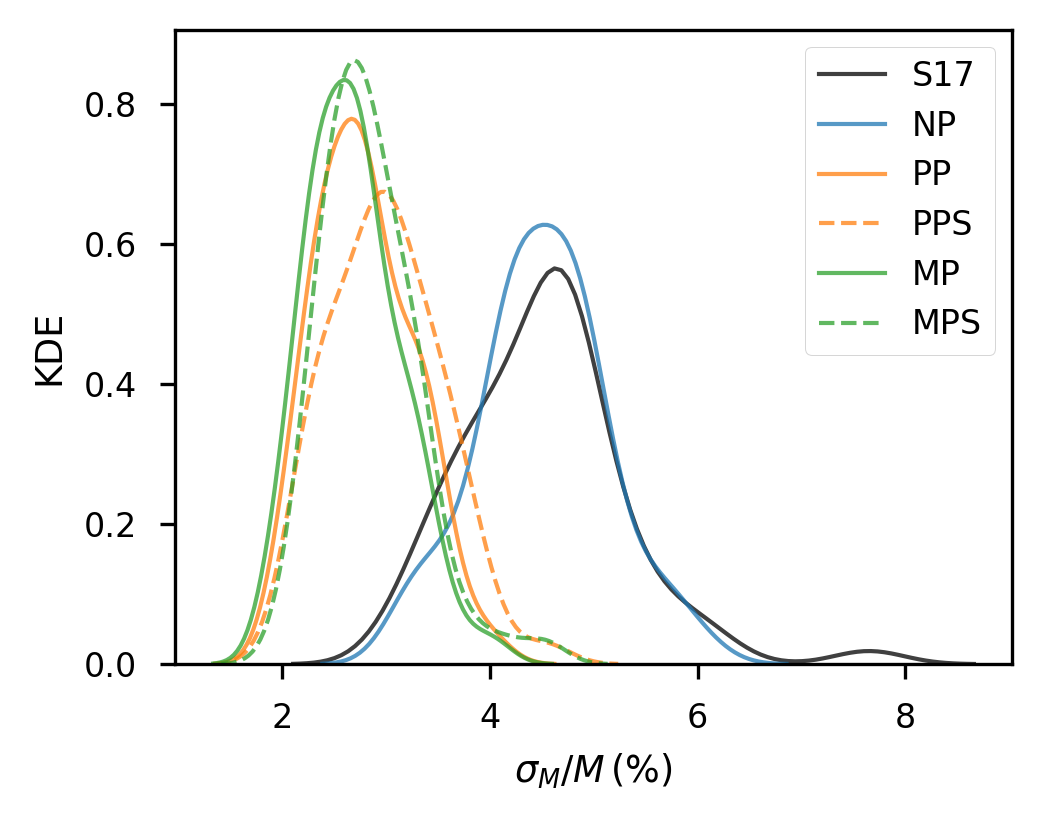
\includegraphics[width=\linewidth]{figures/sigma_mass.png}
%     \end{subfigure}%
%     \begin{subfigure}[b]{.33\linewidth}
%         \centering
%         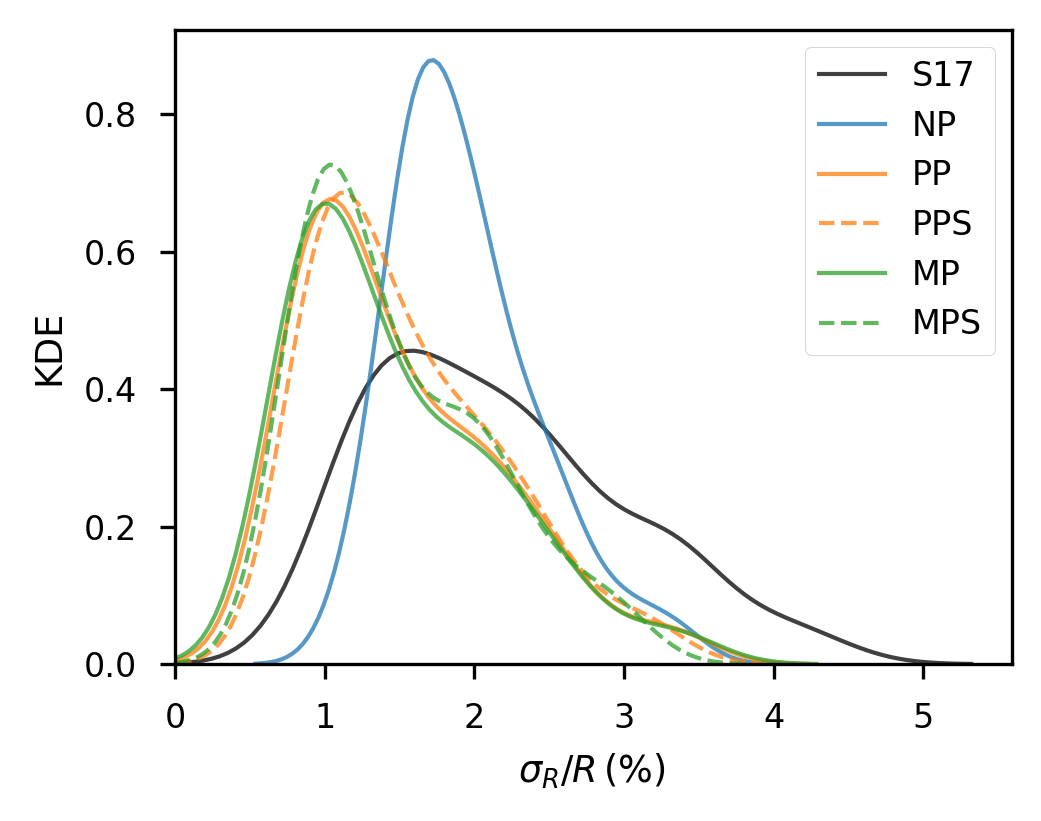
\includegraphics[width=\linewidth]{figures/sigma_rad.png}
%     \end{subfigure}%
%     \begin{subfigure}[b]{.33\linewidth}
%         \centering
%         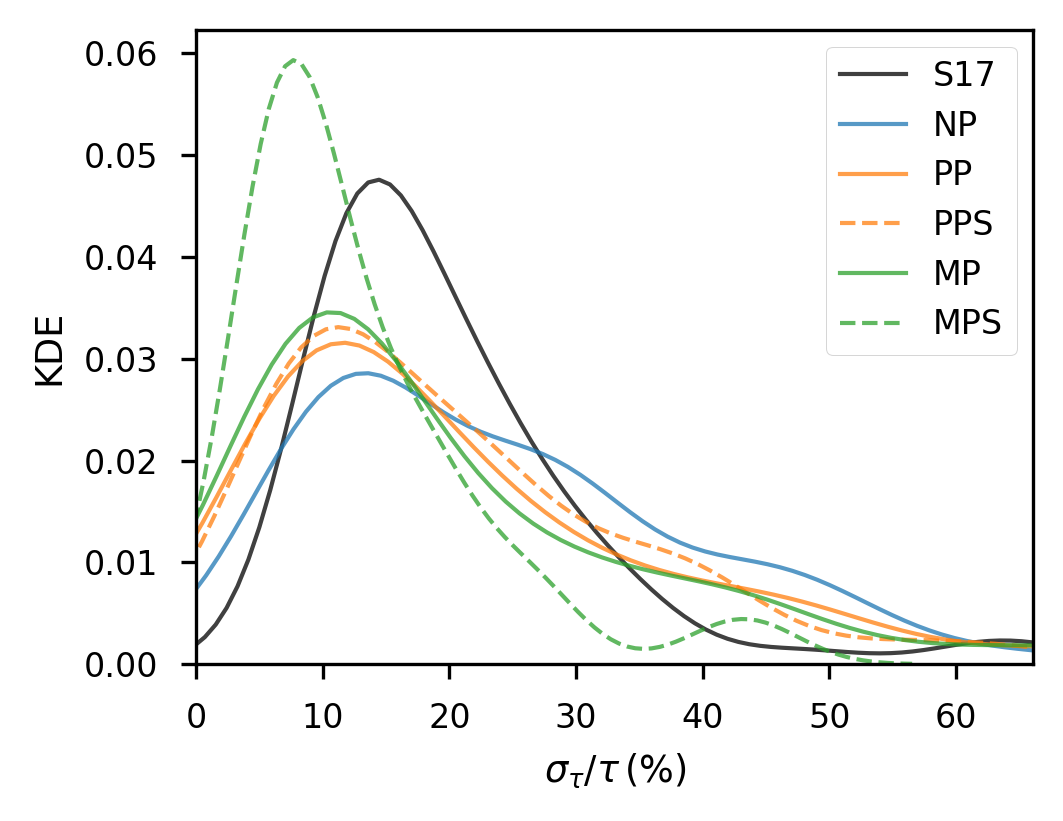
\includegraphics[width=\linewidth]{figures/sigma_age.png}
%     \end{subfigure}%
%     \caption{Kernel density estimates (KDEs) of the distribution of statistical uncertainties in the results from each model compared with those of \citepalias{Serenelli.Johnson.ea2017} for the sample of APOKASC dwarfs and subgiants.}
%     \label{fig:unc-comp}
% \end{figure}

\begin{figure}[!tb]
    \centering
    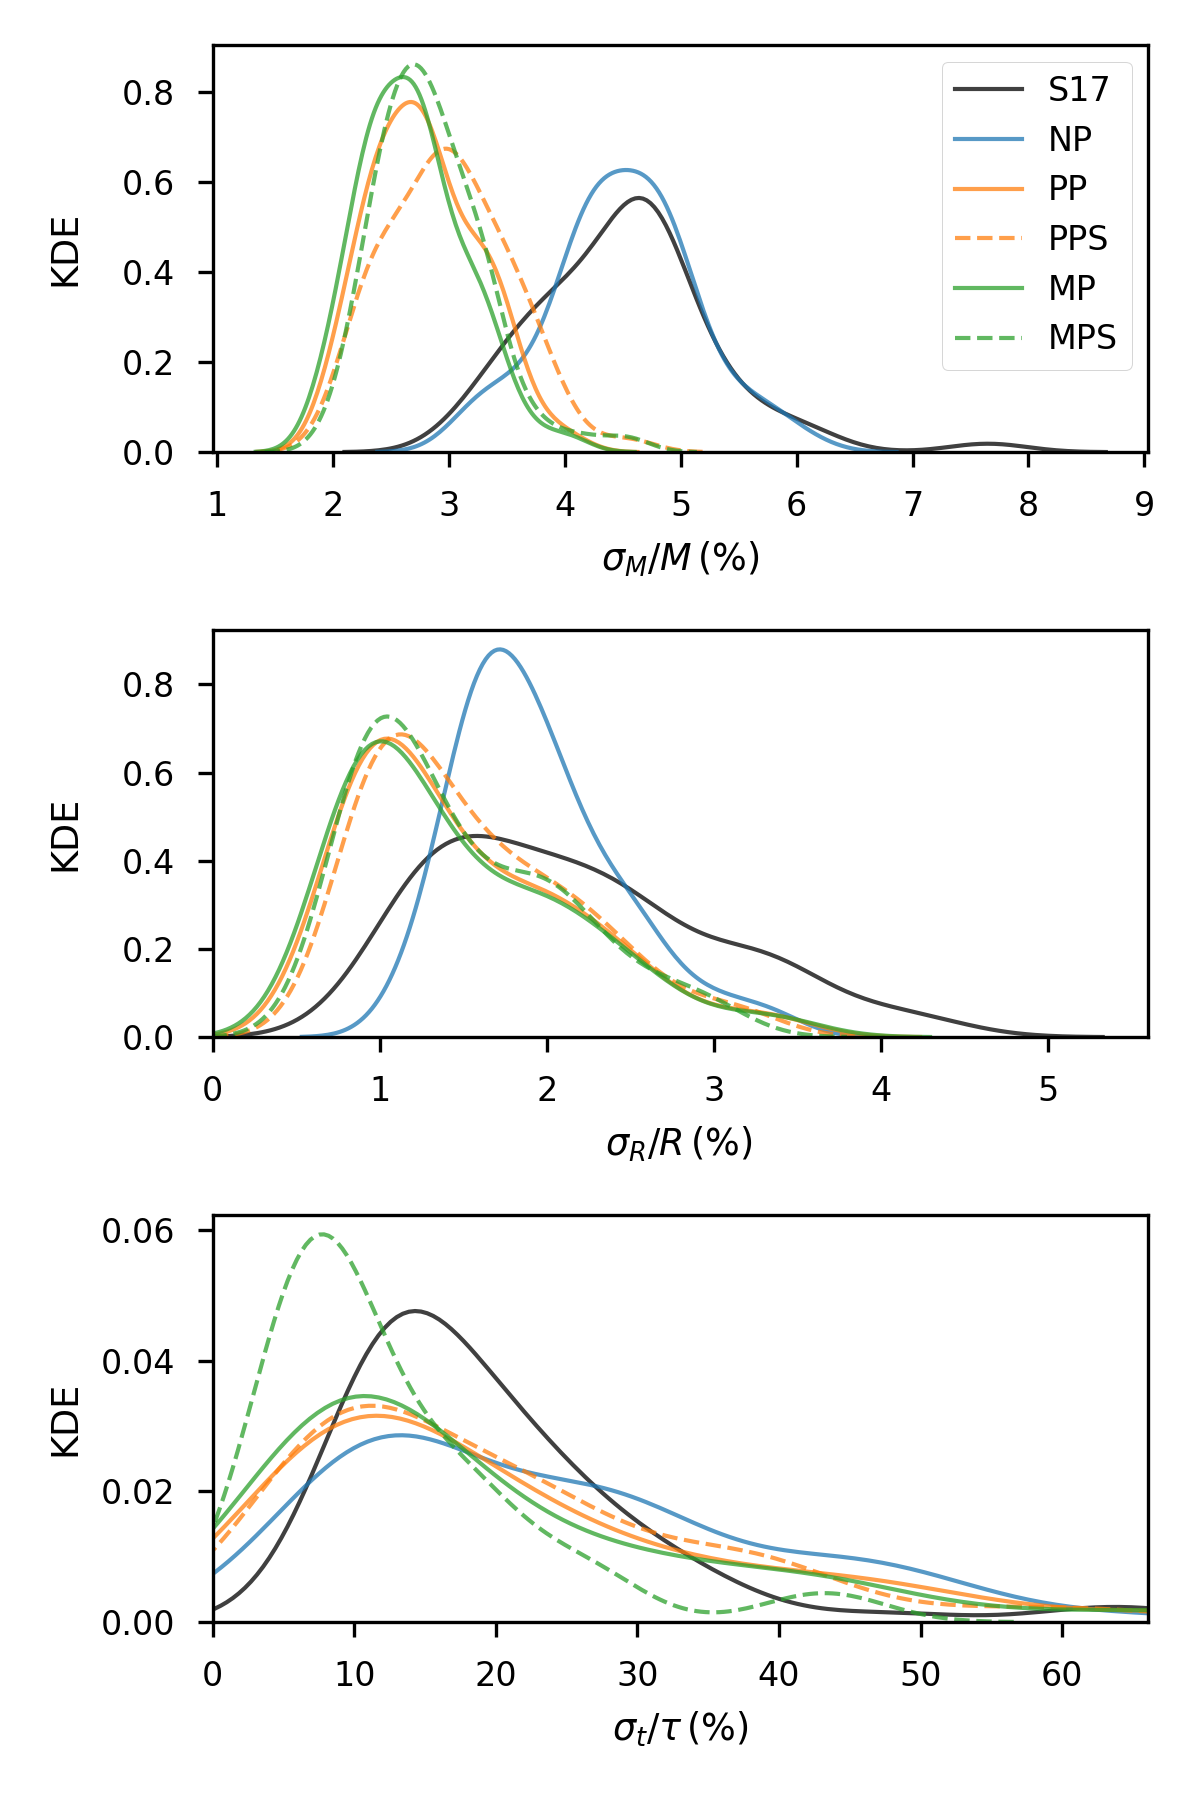
\includegraphics{figures/unc-comp.png}
    \caption[Kernel density estimates of the distribution of statistical uncertainties in the results from each model.]{Kernel density estimates (KDEs) of the distribution of statistical uncertainties in the results from each model compared with those of \citetalias{Serenelli.Johnson.ea2017} for the sample of APOKASC dwarfs and subgiants.}
    \label{fig:unc-comp}
\end{figure}

In Fig. \ref{fig:unc-comp} we compare our statistical uncertainties for $M$, $R$, and $\tau$ with those for the equivalent stars from \citetalias{Serenelli.Johnson.ea2017}. We found that the NP model yielded comparable uncertainties to \citetalias{Serenelli.Johnson.ea2017} but note that these are likely underestimated due the influence of the prior boundaries for $Y_\mathrm{init}$ and $\mlt$. We expected larger uncertainties because we included additional free parameters ($Y_\mathrm{init}$ and $\mlt$) over the work of \citetalias{Serenelli.Johnson.ea2017}. However, when we treat these parameters hierarchically, we saw a reduction in uncertainties from all the pooled models. This is because our prior assumptions about the population allows for the sharing of information between the stars. This uncertainty reduction scales with the number of stars in our sample, demonstrated by the results for the synthetic stars in Fig. \ref{fig:shrinkage}. Thus, hierarchically modelling our population resulted in improved statistical uncertainties in stellar fundamental parameters.

% \begin{figure}
%     \centering
%     \begin{subfigure}[b]{.33\linewidth}
%         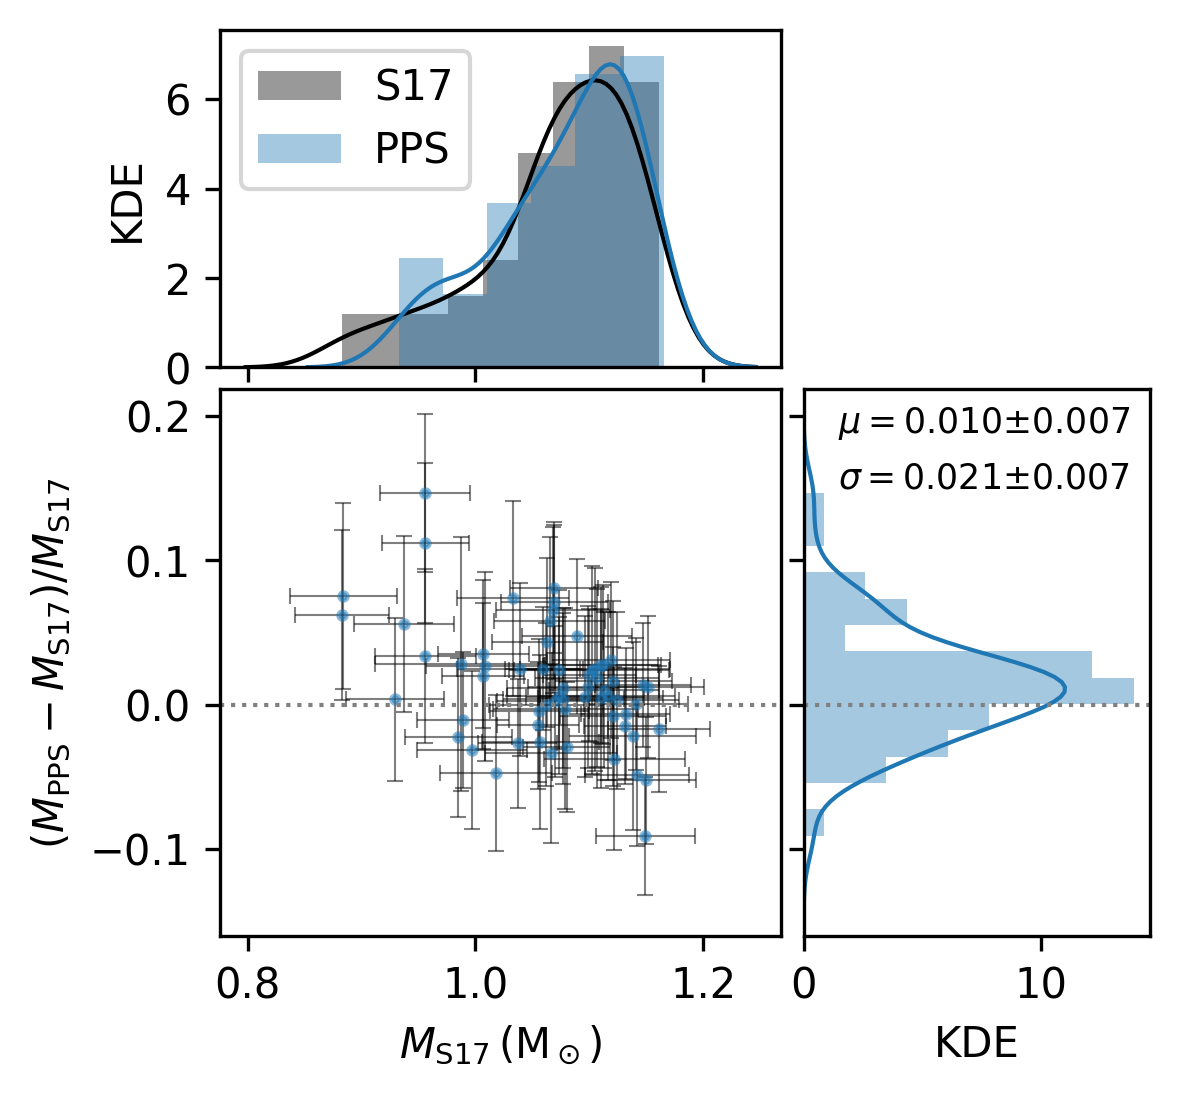
\includegraphics[width=\linewidth]{figures/mass_comp.png}
%     \end{subfigure}%
%     \begin{subfigure}[b]{.33\linewidth}
%         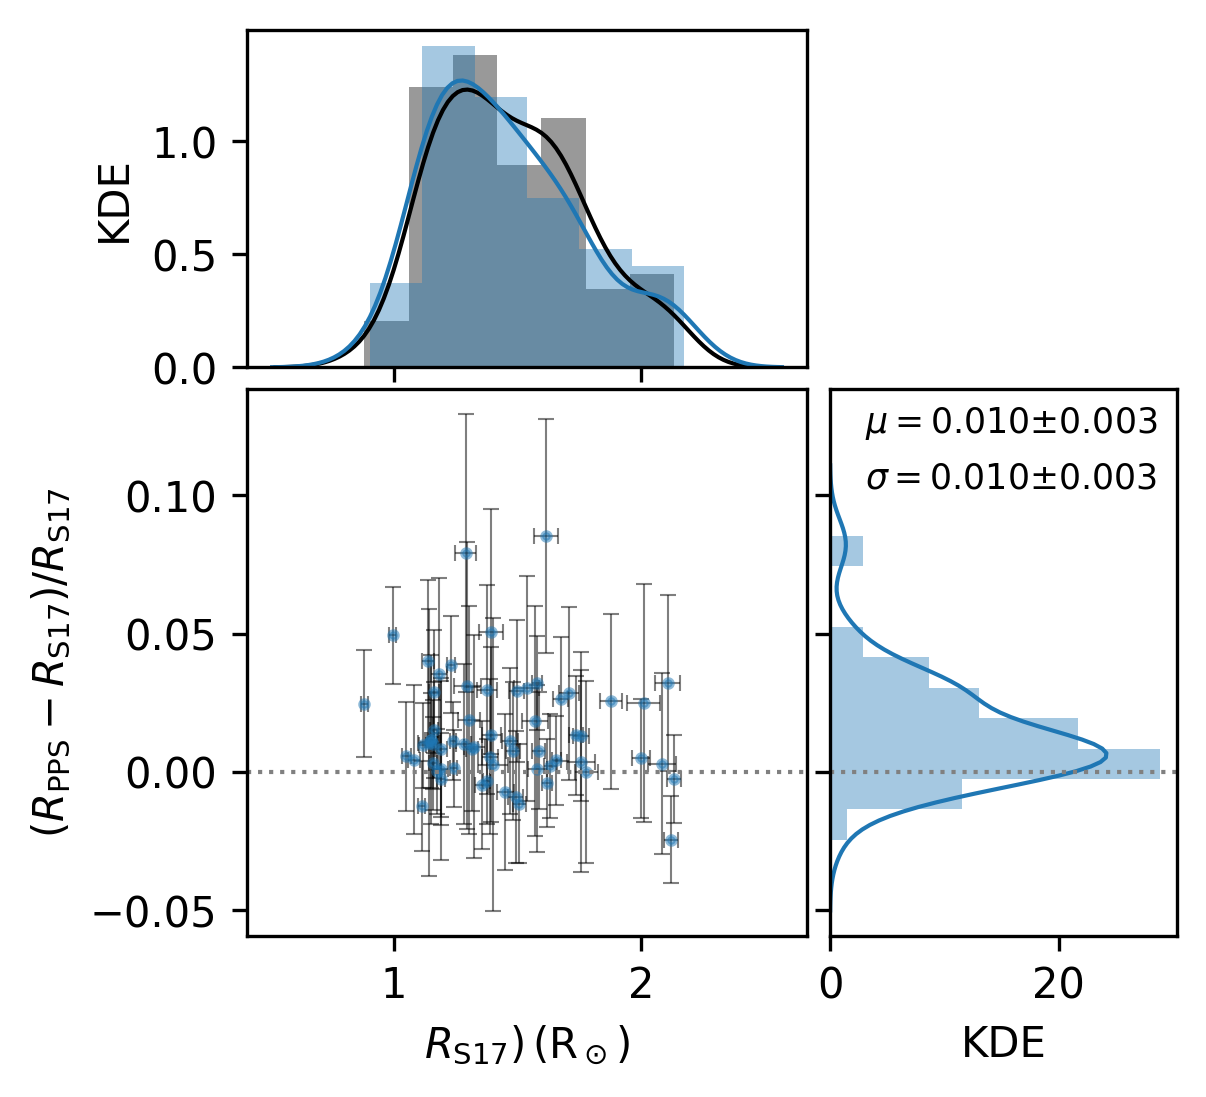
\includegraphics[width=\linewidth]{figures/rad_comp.png}
%     \end{subfigure}%
%     \begin{subfigure}[b]{.33\linewidth}
%         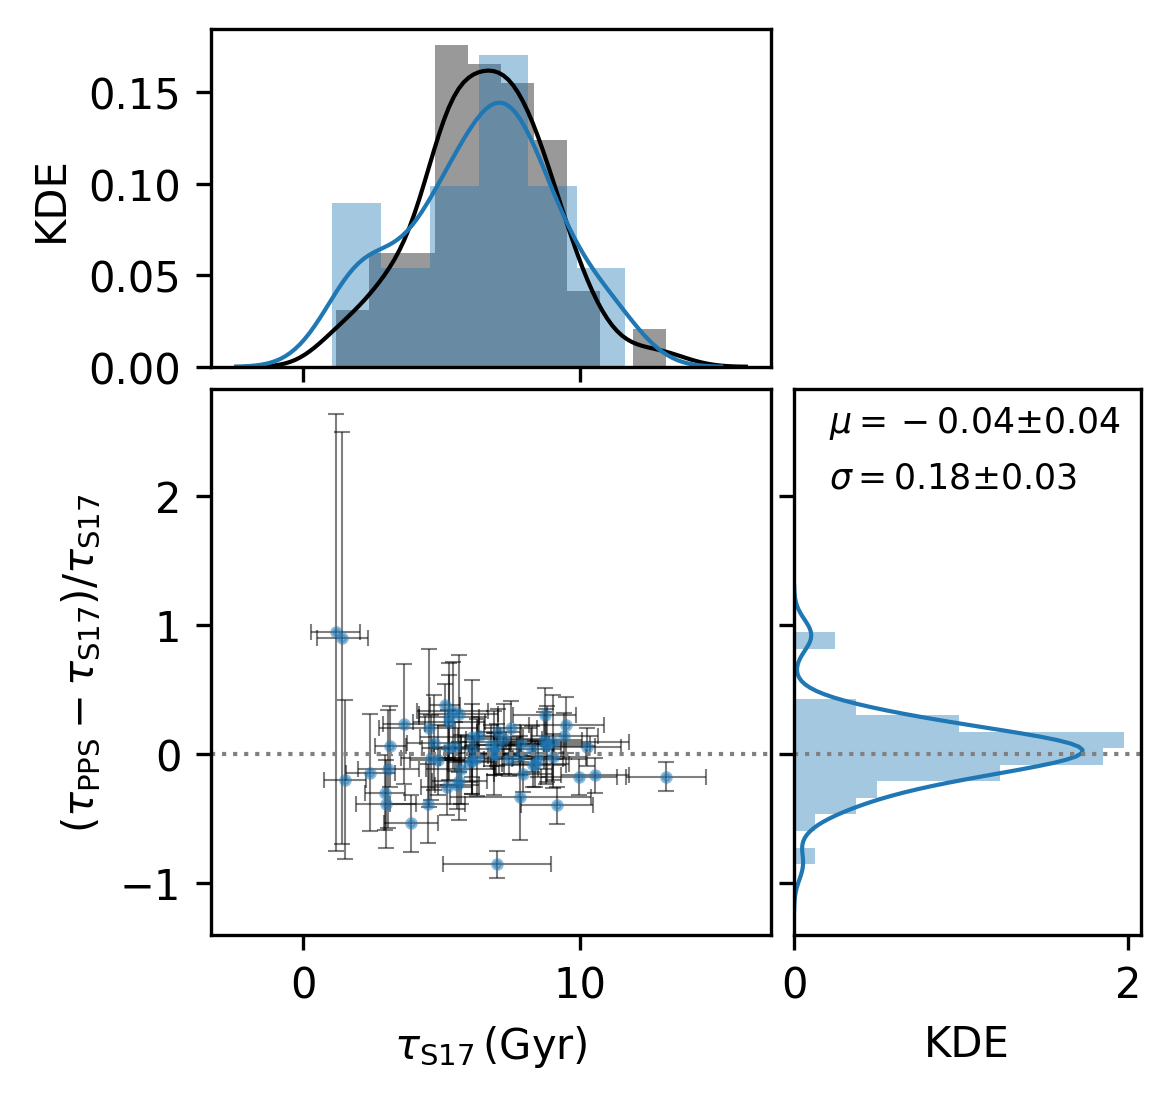
\includegraphics[width=\linewidth]{figures/age_comp.png}
%     \end{subfigure}%
%     \caption{The mean and standard deviation in age, mass and radius results from the PPS model compared with the results (using the photometric temperature scale) from \citetalias{Serenelli.Johnson.ea2017}.}
%     \label{fig:comp}
% \end{figure}

\begin{figure}[!tb]
    \centering
    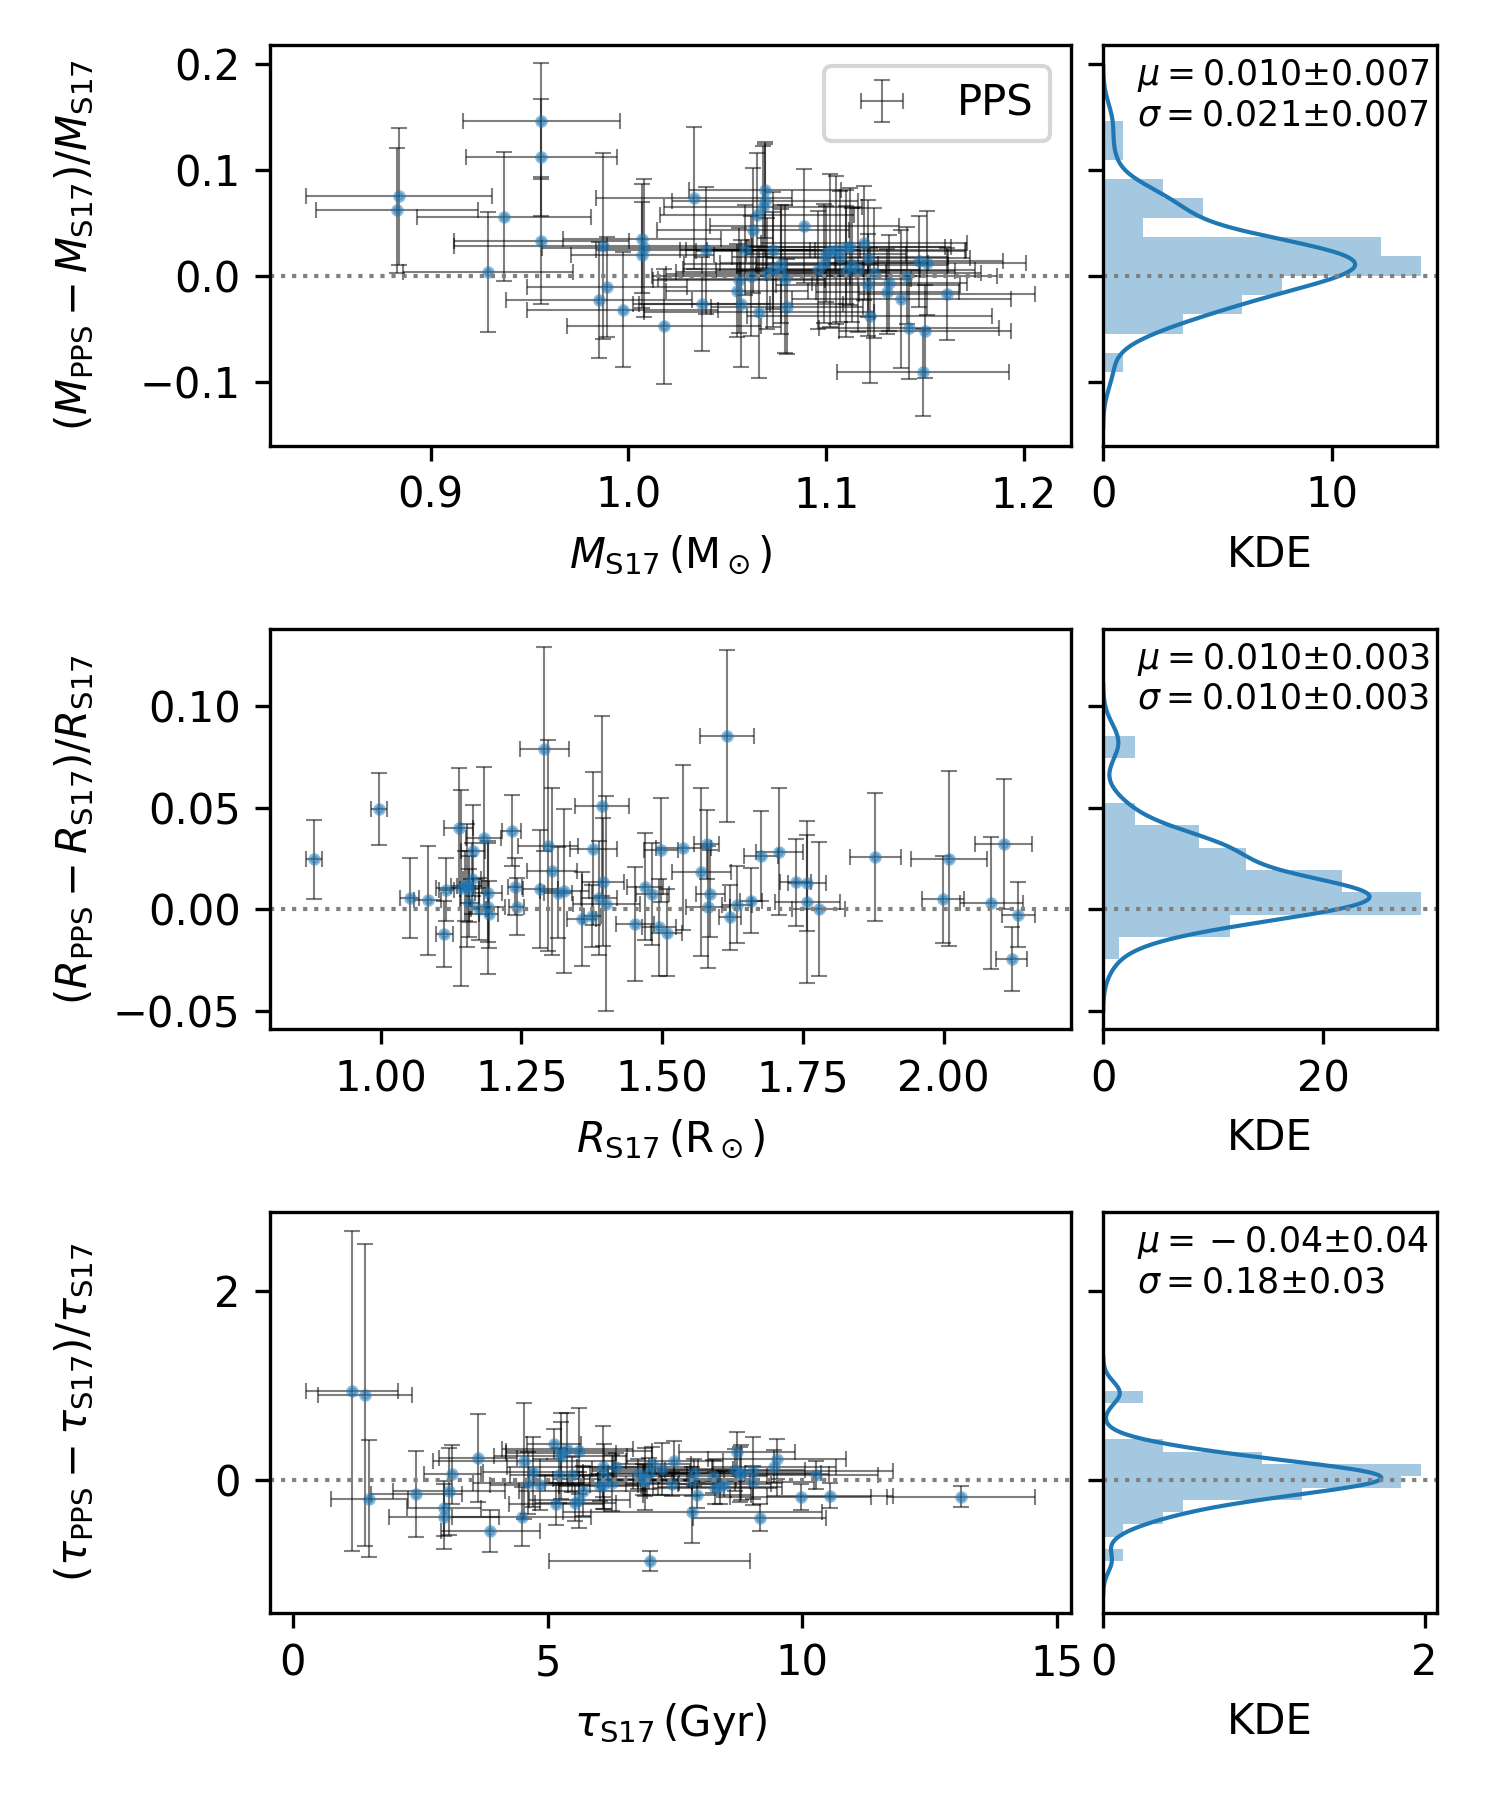
\includegraphics{figures/param-comp.png}
    \caption[The mean and standard deviation in age, mass and radius results from the PPS model.]{The mean and standard deviation in age, mass and radius results from the PPS model compared with the results (using the photometric temperature scale) from \citetalias{Serenelli.Johnson.ea2017}.}
    \label{fig:comp}
\end{figure}

In the following subsection, we compare the results between our PPS model with that of \citetalias{Serenelli.Johnson.ea2017} for mass, radius, and age with reference to Fig. \ref{fig:comp}. We preferred the PPS model for comparison because it utilised the high-precision data available for the Sun as a star to help calibrate the sample, while partially pooling both $Y_\mathrm{init}$ and $\mlt$ to allow for small variations within the population.

\subsubsection{Mass, Radius, and Age}

In the top panel of Fig. \ref{fig:comp}, we compare the masses obtained by the PPS model with \citetalias{Serenelli.Johnson.ea2017} and found a dispersion of around 2 per cent. Our masses were on average 1 per cent above the results from \citetalias{Serenelli.Johnson.ea2017}. Although we might expect the lower $\teff$ scale in this work to underestimate the mass, we attribute this overall effect to our choice of stellar model physics. As previously discussed, the use of \citet{Asplund.Grevesse.ea2009} solar abundances and heavy-element diffusion has the cumulative effect of overestimating stellar masses compared to the physics adopted by \citetalias{Serenelli.Johnson.ea2017}. We also found that the results from all the pooled models returned similar masses, with or without the Sun.

In the central panel of Fig. \ref{fig:comp}, we show that our radii are similar to \citetalias{Serenelli.Johnson.ea2017} with a spread of 1 per cent. We also found radii on average 1 per cent greater than the APOKASC results. Similarly to with mass, this contradicts what would be expected from a lower $\teff$ scale and could also be explained by model physics. Our radii also varied little between models with and without the Sun.

Our ages were also consistent with those from \citetalias{Serenelli.Johnson.ea2017}. The bottom panel of Fig. \ref{fig:comp} shows the spread in the relative age differences to be about 18 per cent, slightly underestimated by 4 per cent. We would expect the lower $\teff$ scale to overestimate the ages as found in \citetalias{Serenelli.Johnson.ea2017}, but instead they are comparable. However, as discussed previously, including diffusion has been shown to reduce age estimates compared to those without. Since we have included diffusion, this could explain the similar ages despite the difference in $\teff$ scale.

Including the Sun in our pooled models affected the resulting ages more than mass and radius. Including the Sun typically overestimated the ages compared to models without the Sun. This is expected given the higher $\mlt$ for the models including solar data, because a larger mixing-length leads to more efficient nuclear burning and more time spent during the MS phase. 

\subsection{Systematic Uncertainties}\label{sec:sys}

We have already accounted for systematics due to the choice of helium enrichment and mixing-length parameter by marginalising over their uncertainties assuming their population distributions. However, there are other model physics which we have not freely varied, including diffusion and choice of solar mixture. Although our method can be adapted to different stellar evolutionary codes and choice of physics, an in-depth analysis of systematic uncertainties is left to future work. 

In previous work studying stars in the APOKASC sample, several pipelines used a range of stellar evolutionary codes and model physics are employed to evaluate systematic uncertainties from the models \citep{Serenelli.Johnson.ea2017, SilvaAguirre.Lund.ea2017}. Using a hierarchical model in this work enabled us to reduce median statistical uncertainties to 2.5 per cent in mass, 1.2 per cent in radius, and 12 per cent in age. However, the systematic uncertainty analysis of \citetalias{Serenelli.Johnson.ea2017} found median systematic uncertainties of 3, 1, and 13 per cent in mass, radius, and age respectively. These are comparable, highlighting the importance of including sources of systematic uncertainty in our model.

Other systematics could arise from observational data. For example, we chose the ASPCAP DR14 $\teff$ scale which was systematically lower than the photometric scale of choice in \citetalias{Serenelli.Johnson.ea2017}. However, our method was still able to recover similar masses, radii, and ages. This could be explained by our choice of stellar model physics, as discussed previously.

\subsection{Outliers}\label{sec:out}

We identified KIC 9025370 as a possible outlier. Consistent across all our models, its modelled effective temperature, $\teff=\SI{5934(50)}{\kelvin}$ was about 4-$\sigma$ greater than its observed $\teff$, and its modelled $L$ was about 2-$\sigma$ dimmer than its observed luminosity. Only $\dnu$ and $\metallicity_\mathrm{surf}$ were consistent between modelled and observed values. The difference was also apparent in our comparison of ages with \citetalias{Serenelli.Johnson.ea2017} where we obtained an age of $1.5\substack{+0.7\\-0.6}\,\si{\giga\year}$ compared to their value of $7.0\substack{+2.0\\-1.6}\,\si{\giga\year}$.

KIC 9025370 turned out to be a double-lined spectroscopic binary \citep{Nissen.SilvaAguirre.ea2017}, discovered after \citetalias{Serenelli.Johnson.ea2017} and hence included in the original sample. The higher observed luminosity from \textsc{Isoclassify} and inconsistent spectroscopic $\teff$ compared with our model posteriors were compatible with a spectroscopic binary. We calculated a photometric $\teff$ using the IRFM method \citep{Casagrande.Ramirez.ea2010} with the available 2MASS photometry for the target and obtained $\teff=\SI{5983(120)}{\kelvin}$, more consistent with our modelled effective temperature and inconsistent with its spectroscopic $\teff$. Thus, our inferred $\teff$ was within the dispersion between different observed $\teff$ scales. Running the model without KIC 9025370 did not affect the resulting inferred hyperparameters, demonstrating the robustness of our model. Therefore, we present KIC 9025370 in our results but suggest that further investigation should be carried out.

\section{Conclusion}

%%%%%%%%%%%%%%%%%%%%%%%%%%%%%%%%%%%%%%%%%%%%%%%%%%

%%%%%%%%%%%%%%%%%%%% CONCLUSION %%%%%%%%%%%%%%%%%%

We have shown that modelling $Y_\mathrm{init}$ and $\mlt$ to improve inference of fundamental parameters can be done through the use of an HBM, whilst still improving statistical uncertainties. Our results were in good agreement with \citetalias{Serenelli.Johnson.ea2017} with small changes in mass and radii expected from our choice of model physics and updated observables. Taking our partially-pooled model including the Sun (PPS) as our preferred set of results, we obtained median statistical uncertainties on $M$, $R$, and $\tau$ of 2.5, 1.2, and 12 per cent respectively. Furthermore, we demonstrated that the uncertainties reduced with increasing sample size in a population of synthetic stars, giving scope to further improve our inference on larger sample sizes from \emph{TESS}.

We found that the gradient, $\Delta Y / \Delta Z$ of the linear helium enrichment law ranged from 0.8 to 1.6 depending on the level of parameter pooling and the inclusion of the Sun in our sample, with $\Delta Y / \Delta Z = 1.1\substack{+0.3\\-0.3}$ from our preferred PPS model. Consistent across our models was the spread in initial helium about the enrichment law, $\sigma_Y = 0.005\substack{+0.004\\-0.003}$. The mean $\mlt$ in the population was $\mu_\alpha = 1.90\substack{+0.10\\-0.09}$ for the PPS model, with values from 1.7 to 2.1 depending on the level of pooling and whether or not solar data was included. We also found the spread in $\mlt$ doubled to $\sigma_\alpha = 0.13\substack{+0.06\\-0.05}$ to account for the addition of the Sun in our sample. We conclude that there are still discrepancies between the best-fitting $\mlt$ in our population and that of the Sun which need to be investigated further. Perhaps, the addition of asteroseismic signatures of helium abundance \citep[see e.g.][and Chapter \ref{chap:glitch}]{Verma.Raodeo.ea2017} would improve our constraints on $Y_\mathrm{init}$ and thus reduce star-by-star uncertainties in $\mlt$.

Using HBMs has allowed us to introduce more free parameters without inflating statistical uncertainties. We used an ANN to approximate stellar models, a method which can be extended to higher input dimensions with little impact on training and evaluation time. Our model also scales well with the number of stars, making use of GPU parallel processing when sampling the posterior.

As shown in tests with synthetic stars (Appendix \ref{sec:test-stars}) and apparent in Fig. \ref{fig:unc-comp}, increasing the number of stars decreases the statistical uncertainties when parameters are pooled. The theoretical limit to this improvement is $\sqrt{N_1 / N_2}$ for two populations of size $N_1$ and $N_2$. For example, if we increase our sample to 300 stars, we would expect the uncertainties to reduce by up to a factor of 2. Naturally, the uncertainty is still limited by observational precision. However, hierarchical modelling as demonstrated in this work, allows us to get the most out of our data and paves the way for a data-driven analysis of model systematics.

Including all-sky data from \emph{TESS} and in anticipation of \emph{PLATO} \citep{Rauer.Catala.ea2014} we can expect our sample size of asteroseismic dwarfs and subgiants only to increase. There is also scope to extend our grid of models to include red giants, for which there are vast catalogues of stars already studied with \emph{Kepler} \citep{Pinsonneault.Elsworth.ea2018}.

% \section*{Acknowledgements}

% %%%%%%%%%%%%%%%%%%%%%%%%%%%%%%%%%%%%%%%%%%%%%%%%%%

% %%%%%%%%%%%%%%%% ACKNOWLEDGEMENTS %%%%%%%%%%%%%%%%

% This work is a part of a project that has received funding from the European Research Council (ERC) under the European Union’s Horizon 2020 research and innovation programme (CartographY; grant agreement ID 804752). A.J.L., G.R.D., and W.J.C. acknowledge the support of the Science and Technology Facilities Council. D.H. acknowledges support from the Alfred P. Sloan Foundation, the National Aeronautics and Space Administration (80NSSC19K0597), and the National Science Foundation (AST-1717000). M.B.N. acknowledges support from the UK Space Agency. R.A.G. acknowledges the funding from the PLATO CNES grant. We acknowledge the use of the \textsc{daft} and \textsc{corner} packages to produce figures in this work. We thank Ilya Mandel and Sean Matt for their discussion regarding this work. We also thank the referee for their immensely helpful comments which have improved the paper.

% \section*{Data Availability}

% %%%%%%%%%%%%%%%%%%%%%%%%%%%%%%%%%%%%%%%%%%%%%%%%%%

% %%%%%%%%%%%%%%% DATA AVAILABILITY %%%%%%%%%%%%%%%%

% The data underlying this article are available in the article, in its online supplementary material, and in Zenodo, at \url{https://dx.doi.org/10.5281/zenodo.4746353}.

  % chapters/glitch.tex
%
% Copyright 2023 Alexander Lyttle.
%
% This work may be distributed and/or modified under the conditions of the
% LaTeX Project Public License (LPPL) version 1.3 or later.
%
% The latest version of this license is in
% https://www.latex-project.org/lppl.txt and version 1.3 or later is part of
% all distributions of LaTeX version 2005/12/01 or later.
%
%
\chapter[Acoustic Glitches in Solar-Like Oscillators]{Acoustic Glitches in Solar-Like Oscillators as a Signature of Helium Abundance}\label{chap:glitch}

% \epigraph{\singlespacing``Ideals are like stars: you will not succeed in touching them with your hands, but like the seafaring man on the ocean desert of waters, you choose them as your guides, and following them, you reach your destiny.''}{\emph{Carl Schurz}}

% So far in this thesis, we have shown that a hierarchical Bayesian model can be used to infer the helium abundance distribution in a stellar population. We also found how this improves the inference of fundamental stellar parameters. However, there is limited information about helium abundance in the stellar observables used (e.g. \(L, \teff, \Delta\nu\)).

An acoustic glitch is a sharp variation of the sound speed inside a medium. The presence of a glitch induces a sinusoidal signature in consecutive standing pressure wave modes. The reason for this is not entirely intuitive, so we go through a simple, one-dimensional example in Section \ref{sec:1d-glitch}. 

Acoustic glitches in Sun-like stars arise from sharp variations in their structure, such as the base of the convection zone (BCZ) and helium ionisation zones (He\,\textsc{i} and He\,\textsc{ii}). Early work identified glitches in solar oscillation modes by analysing their second differences, \(\Delta_2\nu_{nl} \equiv \nu_{n-1\,l} - 2\nu_{nl} + \nu_{n+1\,l}\). Second and higher-order differences remove some smoothly varying components to the mode frequencies and effectively amplify glitch signatures. Assuming a sharp localised discontinuity in sound speed at He\,\textsc{ii} ionisation and the BCZ, \citet{Basu.Antia.ea1994,Basu1997} were able to model these glitches and measure the extent of convective overshoot below the BCZ.

\citet{Monteiro.Thompson1998} further developed a model of the He\,\textsc{ii} ionisation glitch signature by accounting for its finite width in the star, later applying it to study the Sun \citep{Monteiro.Thompson2005}. Around the same time, \citet{Basu.Mazumdar.ea2004} showed the amplitude of the He\,\textsc{ii} glitch signature correlated with the fractional helium abundance (\(Y\)) near the surface of Sun-like stars. Since helium ionises below the stellar atmosphere for these stars, asteroseismology was able to probe where spectroscopy could not. A few years later, \citet{Houdek.Gough2007} proposed a closer physical approximation of the He\,\textsc{ii} glitch. They derived the glitch signature which was later used in many studies of solar-like oscillators.

The glitch could be further studied in stars other than the Sun with the advent of space-based missions. With \emph{CoRoT} providing evidence of solar-like oscillations in red giants, \citet{Miglio.Montalban.ea2010,Mazumdar.Michel.ea2012} found evidence of glitch in red giants. Sample of \emph{Kepler} stars \citep{Mazumdar.Monteiro.ea2012,Mazumdar.Monteiro.ea2014,Verma.Raodeo.ea2017} compare fitting directly and to second differences. For example, 16 Cyg A and B \citet{Verma.Faria.ea2014}. Then \citet{Verma.Raodeo.ea2019} extended this to model to determine helium abundances. Using a variety of stellar models they were not able to find a consistent helium enrichment law.

In Section \ref{sec:glitch-star}, we demonstrate how glitches in stellar structure due to helium ionisation and the BCZ affect the mode frequencies of solar-like oscillators. Starting with the variational principle \citep{Chandrasekhar1964}, we show how to get to the He\,\textsc{ii} glitch signature formula from \citet{Houdek.Gough2007}. Hence, this chapter serves as a primer for Chapter \ref{chap:glitch-gp}, where we apply a new model for measuring acoustic glitches in \(\nu_{nl}\) using a Gaussian process.

\section[1D example]{A One-Dimensional Example of a Glitch}\label{sec:1d-glitch}

\newcommand*{\glitch}{\ensuremath{{\mathrm{g}}}}

A rapid variation in the structure of a medium induces a periodic perturbation (\(\delta\omega\)) to the eigenfrequencies. To demonstrate this, we will explore a simple one-dimensional example \citep[e.g][]{Verner2005}. Consider a medium bound from \(x=0\) to \(x=L\) in which pressure waves can propagate at constant speed \(c\). The longitudinal displacement of the wave \(\xi\) must obey the wave equation,
%
\begin{equation}
    \frac{\partial^2\xi(x, t)}{\partial t^2} = c^2 \frac{\partial^2\xi(x, t)}{\partial x^2},
\end{equation}
%
at a given position \(x\) and time \(t\). A general solution to the wave may be written as a sum of right- and left-travelling waves. In terms of the angular frequency \(\omega\), wave number \(k\), and complex coefficients \((A, B)\),
%
\begin{equation}
    \xi(x, t) = A \ee^{i (\omega t - k x)} + B \ee^{i (\omega t + k x)},
\end{equation}
%
where \(\omega\) and \(k\) satisfy \(\omega = c k\). Solving for the boundary condition \(\xi(0, t) = 0\) we find \(B = - A\). Substituting Euler's formula, \(A = (r/2) \ee^{i\phi}\), we can write the real solution for \(\xi\) as,
%
\begin{equation}
    \real\left[\xi(x, t)\right] = r \sin k x \sin(\omega t + \phi),
\end{equation}
%
representing the physical component of the wave, where \(r\) and \(\phi\) are the amplitude and temporal phase respectively. Solutions for \(\omega\) which satisfy \(\xi(L, t)=0\) may then be found,
%
\begin{equation}
    \omega_n = c \frac{n \pi}{L}, \label{eq:omega-n}
\end{equation}
%
where \(n\) is a non-zero integer (the \(n=0\) solution would give \(\xi=0\) everywhere).

\begin{figure}[!tb]
    \centering
    % 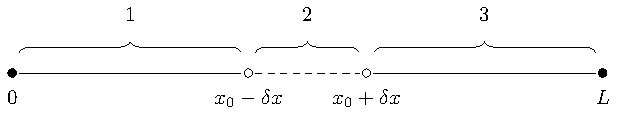
\includegraphics{figures/glitch-1d-example-diagram.pdf}
    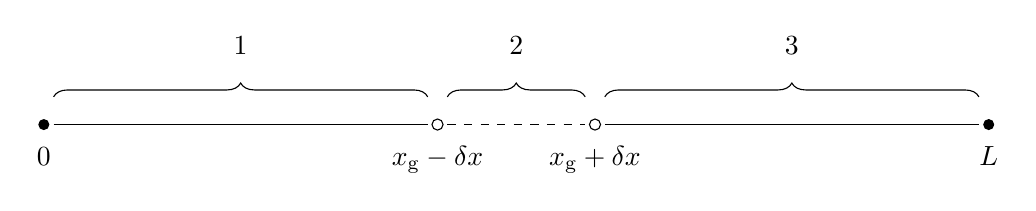
\begin{tikzpicture}
  \def\labelshift{(0, -0.4)}%
  \def\regionshift{(0, 1)}%
  \node[label={[anchor=base,shift=\labelshift]below:0}] (A) at (0, 0) {};
  \node[label={[anchor=base,shift=\labelshift]below:$x_{\mathrm{g}}-\delta x$}] (B) at (5, 0) {};
  \node[label={[anchor=base,shift=\labelshift]below:$x_{\mathrm{g}}+\delta x$}] (C) at (7, 0) {};
  \node[label={[anchor=base,shift=\labelshift]below:$L$}] (D) at (12, 0) {};

  \fill (A) circle (2pt) (D) circle (2pt);
  \draw (B) circle (2pt) (C) circle (2pt);
  \draw (A) -- (B) (C) -- (D);
  \draw[dashed] (B) -- (C);

  \draw[decorate,decoration={brace,amplitude=5pt,raise=10pt}] (A) -- (B) node[midway,shift=\regionshift]{1};
  \draw[decorate,decoration={brace,amplitude=5pt,raise=10pt}] (B) -- (C) node[midway,shift=\regionshift]{2};
  \draw[decorate,decoration={brace,amplitude=5pt,raise=10pt}] (C) -- (D) node[midway,shift=\regionshift]{3};
\end{tikzpicture}

    \caption[A diagram showing a one-dimensional medium with a small structural perturbation.]{A diagram showing a one-dimensional medium split into three regions. 1: Fixed at \(x=0\) with a constant speed of sound \(c\); 2: A small structural perturbation centred at \(x=x_\glitch\) with width \(2\delta x\) and constant speed of sound \(c + \delta c\); 3: Fixed at \(x=L\) with a constant speed of sound \(c\).}
    \label{fig:1d-diagram}
\end{figure}

Now, let us suppose there is a small structural perturbation (or glitch) in the medium at position \(x_\glitch\) with half-width \(\delta x\). Figure \ref{fig:1d-diagram} shows this system divided into 3 regions, with region 2 containing the glitch. In region 2, the speed of sound is \(c + \delta c\) and the corresponding wave number is \(k + \delta k\). We want to find the frequencies which correspond to standing waves in this system and compare them to that of the homogeneous medium above. We will show that the resulting perturbation to the eigenfrequencies (\(\delta\omega\)) is periodic, with an amplitude and period that relates to the properties of the glitch.

Firstly, we propose solutions to the wave for each region by considering reflection and transmission at each boundary. Initially ignoring the wave superposed by a reflection at \(x=L\),
%
\begin{align}
    \xi_1(x, t) &= \ee^{i(\omega t - k x)} + A \ee^{i(\omega t + k x)}, \label{eq:xi1-r} \\
    \xi_2(x, t) &= B\ee^{i(\omega t - (k + \delta k) x)} + C \ee^{i(\omega t + (k + \delta k) x)}, \label{eq:xi2-r} \\
    \xi_3(x, t) &= D \ee^{i(\omega t - k x)}, \label{eq:xi3-r}
\end{align}
%
where complex coefficients \(A\) and \(C\) represent reflections, and \(B\) and \(D\) represent transmissions, at \(x_\glitch \pm \delta x\) respectively. Later, we will substitute the left-travelling wave (\(- \xi\{-k, -\delta k\}\)) after determining the values of the coefficients.

The internal boundary conditions for this system are found by enforcing spacial continuity at \(x - \delta x\) and \(x + \delta x\),
%
\begin{align*}
    \xi_1(x_\glitch - \delta x, t) &= \xi_2(x_\glitch - \delta x, t), \\
    \xi_2(x_\glitch + \delta x, t) &= \xi_3(x_\glitch + \delta x, t), \\
    \frac{\partial \xi_1}{\partial x}(x_\glitch - \delta x, t) &= \frac{\partial \xi_2}{\partial x}(x_\glitch - \delta x, t), \\
    \frac{\partial \xi_2}{\partial x}(x_\glitch + \delta x, t) &= \frac{\partial \xi_3}{\partial x}(x_\glitch + \delta x, t).
\end{align*}
%
Solving these simultaneously with the Python package \textsc{sympy} gives the following equations for the complex coefficients\footnote{The code for these derivations are available at \url{\gitremote/tree/\gitbranch/notebooks}},
%
\begin{align}
    A &= \delta k (2k + \delta k) (1 - \ee^{4i \delta x (k + \delta k)}) \ee^{- 2i k (x_\glitch - \delta x)} \alpha^{-1}, \\
    B &= 2 k (2k + \delta k) \ee^{4i \delta x (k + \delta k)} \ee^{i \delta k (x_\glitch - \delta x)} \alpha^{-1}, \\
    C &= 2 k \delta k \ee^{- i (x_\glitch - \delta x) (2k + \delta k)} \alpha^{-1}, \\
    D &= 4 k (k + \delta k) \ee^{2 i \delta x (2k + \delta k)} \alpha^{-1},
\end{align}
%
where,
\begin{equation}
    \alpha = (2k + \delta k)^2 \ee^{4 i \delta x (k + \delta k)} - \delta k^2.
\end{equation}
%

Now we have solutions for the coefficients, we can superpose the right-travelling wave, \(\xi\{k, \delta k\} \rightarrow - \xi\{-k, -\delta k\}\) to get the full solution for the wave function. Substituting \(k \rightarrow -k\) and \(\delta k \rightarrow -\delta k\) into the coefficients yields their complex conjugates, \((\overline{A},\overline{B},\overline{C},\overline{D})\). This allows us to rewrite the wave functions into a more flexible form. For example, substituting Euler's formula, \(A = (r_A/2) \ee^{i\phi_A}\) and \(\overline{A} = (r_A/2) \ee^{-i\phi_A}\), Equation \ref{eq:xi1-r} now becomes,
%
\begin{equation}
    \xi_1(x, t) = \ee^{i \omega t} \left[ \frac{r_A}{2} \left( \ee^{i(kx + \phi_A)} - \ee^{-i(kx + \phi_A)} \right) - \left( \ee^{ikx} - \ee^{-ikx} \right) \right], \label{eq:xi1}
\end{equation}
%
where its real component is,
\begin{equation}
    \real\left[\xi_1(x, t)\right] = \sin \omega t \left[2 \sin kx - r_A \sin(kx + \phi_A)\right].
\end{equation}
%
However, this does not satisfy the outer boundary condition that the displacement is always zero at \(x=0\); in other words, \(\xi_1(0, t) = - r_A \sin \omega t \sin(\phi_A) \neq 0\) everywhere. To fix this, we introduce a small displacement phase \(\epsilon\) caused by the glitch, and let \(x \rightarrow x + \epsilon\). We will determine \(\epsilon\) shortly. In the meantime, superposing the right-travelling wave and substituting Euler's formula into Equations \ref{eq:xi2-r} and \ref{eq:xi3-r}, we can write the real components of the wave functions,
%
\begin{align}
    \real[\xi_1(x, t)] &= \sin \omega t \left\{2 \sin[k (x + \epsilon)] - r_A \sin[k(x + \epsilon) - \phi_A]\right\} \label{eq:xi1-real} \\
    \real[\xi_2(x, t)] &= \sin \omega t \left\{ r_B \sin[(k + \delta k)(x + \epsilon) - \phi_B] - r_C \sin[(k + \delta k)(x + \epsilon) - \phi_C]\right\} \\
    \real[\xi_3(x, t)] &= \sin \omega t \left\{r_D \sin[k(x + \epsilon) - \phi_D]\right\} \label{eq:xi3-real}
\end{align}
%
Imposing the boundary condition \(\xi_1(0, t) = 0\), we solve Equation \ref{eq:xi1-real} for \(\epsilon\) at \(x=0\),
%
\begin{align}
    \epsilon &= \frac{1}{k} \tan^{-1}\left( \frac{(r_A / 2) \sin(\phi_A)}{1 - (r_A/2) \cos(\phi_A)} \right), \notag\\
    &= \frac{1}{k} \tan^{-1}\left( \frac{\imag[A]}{1 - \real[A]} \right). \label{eq:1d-phase}
\end{align}
%

Finally, we can impose the boundary condition \(\xi_3(L, t) = 0\) to solve for \(\omega\). Setting Equation \ref{eq:xi3-real} to zero, we can rewrite it in terms of the real and imaginary components of \(D\),
%
\begin{align}
    \sin \omega t \left\{r_D \sin[k(L + \epsilon) - \phi_D]\right\} &= 0, \quad (\div \sin \omega t) \notag \\
    r_D \cos \phi_D \sin[k(L + \epsilon)] - r_D \sin \phi_D \cos[k(L + \epsilon)] &= 0, \notag \\
    \real[D] \sin[k(L + \epsilon)] - \imag[D] \cos[k(L + \epsilon)] &=0. \label{eq:1d-glitch-sol}
\end{align}
%
The glitch affects the amplitude and phase of the wave. If we set \(\epsilon = 0\) and \(D = 1\) we recover the homogeneous frequency solutions (Equation \ref{eq:omega-n}). Unfortunately, solving Equation \ref{eq:1d-glitch-sol} for \(\omega\) is not possible analytically. However, we can find individual roots (or oscillation modes) numerically.

\begin{figure}
    \centering
    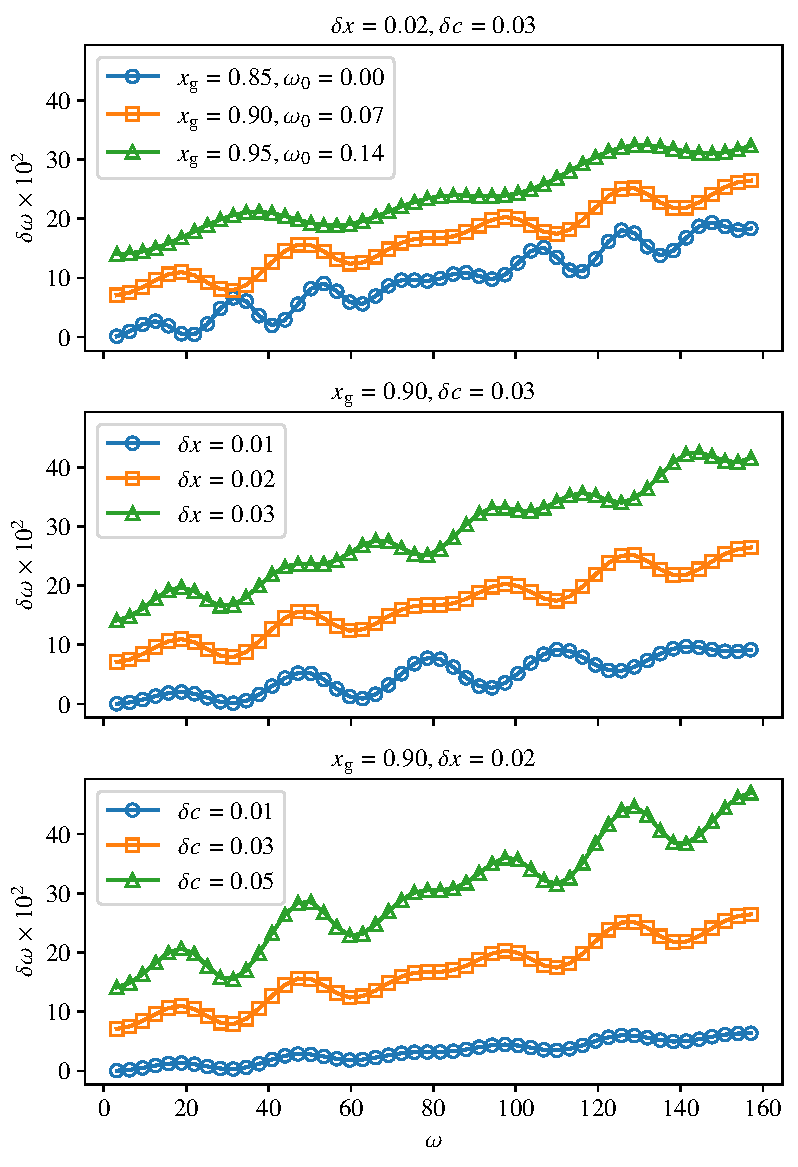
\includegraphics{figures/glitch-1d-example-results.pdf}
    \caption{The change in mode frequency induced by a change in sound speed of \(\delta c\) from \(x_\glitch - \delta x\) to \(x_\glitch + \delta x\) in a one-dimensional medium, bound such that \(x \in [0, 1]\) (see Figure \ref{fig:1d-diagram}). Outside of the perturbation the speed of sound, \(c=1\).
    The frequencies in the top panel are offset by \(\omega_0\).
    Points are joined by straight lines to guide the eye.
    }
    \label{fig:1d-results}
\end{figure}

Let us use \(\omega'_n\) to denote the solutions to Equation \ref{eq:1d-glitch-sol}, where \(n\) is a positive integer. We find \(\omega'_n\) by solving Equation \ref{eq:1d-glitch-sol} using Newton's method for \(n = 1,\dots,50\). Using dimensionless units of length and time, we set \(c=1\), \(L=1\), and test several values of \(x_\glitch\), \(\delta x\), and \(\delta c\). Initial guesses for \(\omega'_n\) are obtained from the homogeneous medium solutions in Equation \ref{eq:omega-n}. The difference between the solutions for \(\omega'_n\) and those from the homogeneous medium, \(\delta \omega_n = \omega'_n - \omega_n\), are shown in Figure \ref{fig:1d-results}. We can see a periodic component of \(\delta\omega\) induced by the glitch. Physically, this arises from the change in phase required to satisfy the boundary conditions of the glitch region. As the wave nodes pass in and out of the region with changing \(n\), the sensitivity of the wave to the glitch oscillates. The overall sensitivity to the glitch depends on how much the wave changes inside the glitch, hence why low \(n\) modes have smaller \(\delta\omega\).

The functional form of \(\delta\omega\) appears to have a linear component and a short period oscillation modulated by a longer period. As the location of the glitch (\(x_\glitch\)) gets smaller, the short period of \(\delta\omega\) decreases. If we imagine the spacial distribution of nodes in the system as a function of \(n\), the density of nodes is larger towards the centre of the system. The periodicity arises from the nodes passing in and out of the glitch region with changing \(n\). Therefore, where the density of wave nodes is higher, we expect the short period of \(\delta\omega\) to decrease. Similarly, as the the half-width of the glitch (\(\delta x\)) increases, the longer period increases. 

Furthermore, an increasing change in sound speed (\(\delta c\)) increases the amplitude of \(\delta\omega\). This result is intuitive, as we expect a perturbation in \(c\) to be proportional to a perturbation in \(\omega\). Finally, increasing both \(\delta x\) and \(\delta c\) increases the slope of \(\delta\omega\). The sensitivity of a mode to the glitch increases with \(n\) and depends on how much the wave changes in the glitch region. A larger glitch allows modes of smaller \(n\) to `see' the glitch region, thus increasing the linear slope of \(\delta\omega\).

%This may be interpreted as the nodes of each standing wave passing in and out of region 2 with increasing \(n\). Where there is a node, the wave is least sensitive to a change in structure, and 

\begin{figure}
    \centering
    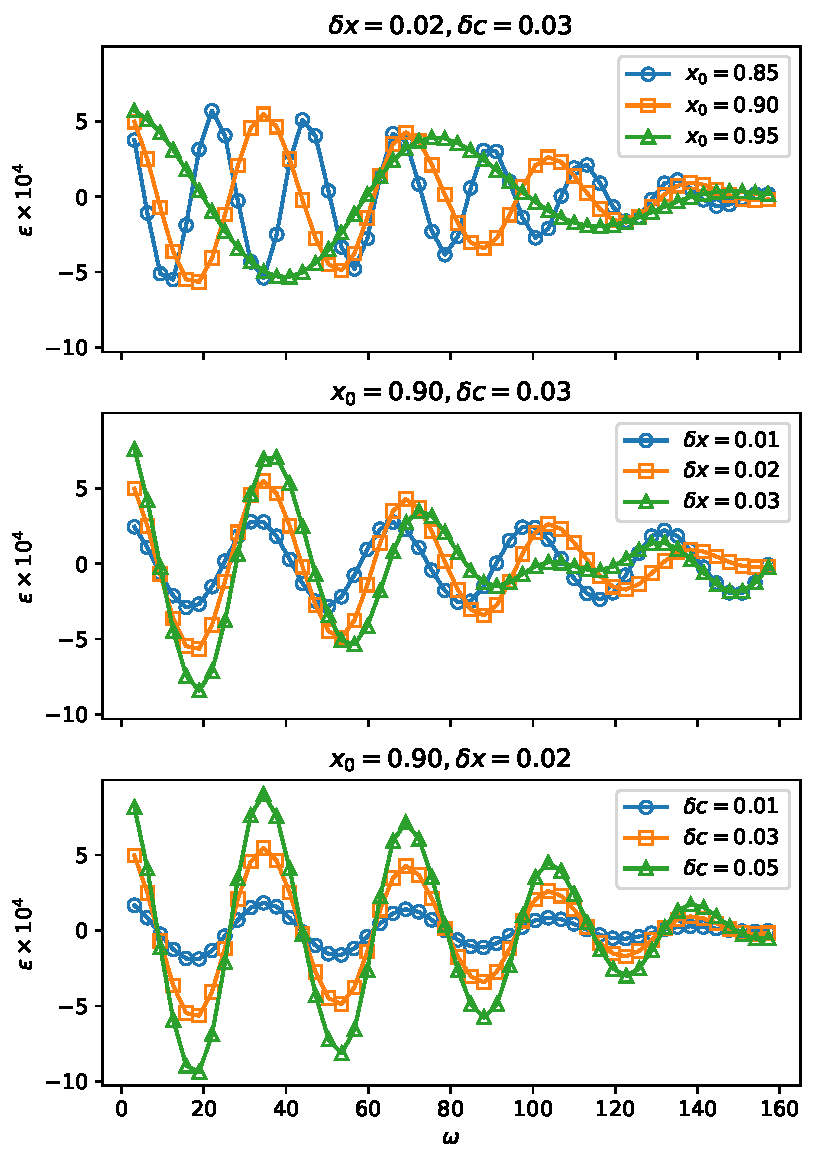
\includegraphics{figures/glitch-1d-example-phase.pdf}
    \caption{The same as Figure \ref{fig:1d-results} but showing the phase offset \(\epsilon\) required to satisfy the boundary conditions.}
    \label{fig:1d-phase}
\end{figure}

The small phase offset \(\epsilon\) in Equation \ref{eq:1d-phase} is required for the wave function to satisfy the boundary conditions at \(x = 0\). However, adding \(\epsilon\) shifts the effective location of \(x_\glitch\) --- it changes the scale of the \(x\)-axis by a factor of \((1 + \epsilon)\). We plot \(\epsilon\) against \(\omega\) in Figure \ref{fig:1d-phase} and show that its magnitude is \(\sim 10^{-4}\), much smaller than the location and size of region 2. The periodicity caused by the glitch also shows up in Figure \ref{fig:1d-phase}, with its properties affected in a similar way to Figure \ref{fig:1d-results}.

Finding an approximate solution for \(\delta\omega\) is beyond the scope of this example. However, we can show that by modelling \(\delta\omega\), we can recover information about the structural glitch. Let us build a model \(\delta\omega = f(\omega)\). Looking at Figure \ref{fig:1d-results}, we propose a form for \(f\),
%
\begin{equation}
    f(\omega) = a_1 \omega - a_2 \sin (\tau_1 \omega) \cos (\tau_2 \omega), \label{eq:1d-domega-func}
\end{equation}
%
where \(a_1\) and \(a_2\) are coefficients which are both functions of \(\delta x\) and \(\delta c\). Parameters \(\tau_1\) and \(\tau_2\) are the `frequencies' (with dimensionless units of time\footnote{An angular frequency in angular frequency space has units of time.}) of the periodic component to \(\delta\omega\), which are functions of \(\delta x\) and \(x_\glitch\) respectively.

\begin{figure}[tb]
    \centering
    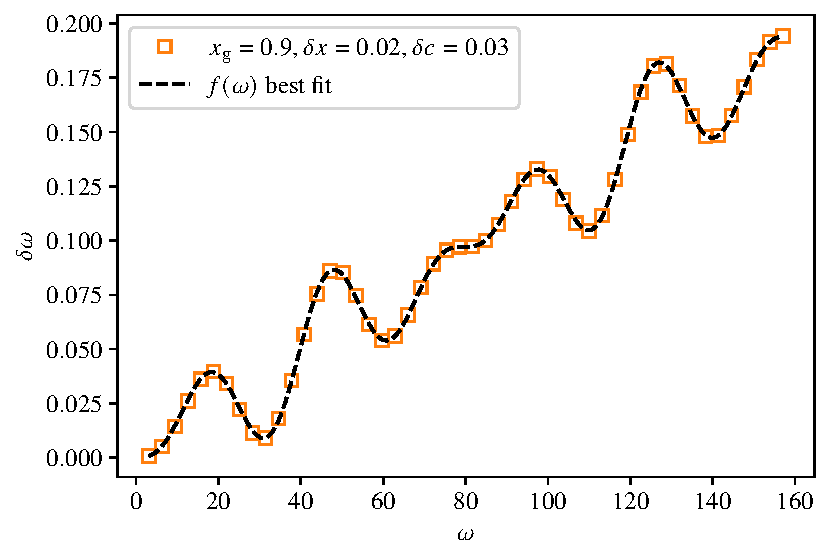
\includegraphics{figures/glitch-1d-fit.pdf}
    \caption{Best fit of Equation \ref{eq:1d-domega-func} to \(\delta\omega_n\) for \(n=1,\dots,50\), \(L=1\), and \(c=1\).}
    \label{fig:1d-fit}
\end{figure}

We fit Equation \ref{eq:1d-domega-func} to \(\delta\omega_n\) obtained from a glitch located at \(x_\glitch = 0.9\), with half-width \(\delta x = 0.02\), and change in sound speed \(\delta c = 0.03\). The best fitting line is shown in Figure \ref{fig:1d-fit}. We found \(\tau_1 \approx \num{0.0389}\) and \(\tau_2 \approx \num{0.199}\). This corresponded to \(\tau_1 \simeq 2\delta\tau\), where \(\delta\tau\) is half the acoustic width of the glitch --- the time at which sound takes to transverse the region. Since the speed of sound \(c \approx \num{1}\) throughout the medium, the true value of \(\delta\tau = 0.02\). We also found the second `frequency' \(\tau_2 \simeq 2\tau_\glitch\), where \(\tau_\glitch\) is the sound travel time from the nearest edge to the centre of the glitch (in this case \num{0.1}). Referring back to Figure \ref{fig:1d-results}, we can infer that the relation between parameters of Equation \ref{eq:1d-domega-func} and the glitch should approximately hold for different values of \(x_\glitch\), \(\delta x\), and \(\delta c\).

% NOTE: Could take this further to show a1 = 2 dc dtau / L and a2 = dc / L

It would be tempting to test this further, but we have shown that modelling the signature of a glitch (\(\delta\omega\)) can help characterise its properties. Although the structure of a star is more complicated than this example, we can extend this principle to find glitch signatures in the mode frequencies of solar-like oscillators. Therefore, we will build upon this analogy and explore acoustic glitches in stars in the next section.

% NOTES: Go slowly through this. The next step is to fit a simple mode to theses oscillations and show that we can find x0 and dx. And show how the amplitude scales with dc.

% NOTES: When it comes to fitting the helium glitch, consider first fitting a GP to the modes with a free noise term. Fix the kernel scale to a series of values and show that we can see the glitch in the residuals. Of course, this leaves the question of what kernel scale to use. Well, we could just model everything at once!

\section[Glitches in Stars]{Acoustic Glitches in Solar-Like Oscillators}\label{sec:glitch-star}

In the previous section, we considered a glitch in a homogeneous medium, where the speed of sound is constant everywhere else. In a star, the adiabatic sound speed is not constant. It depends on the density (\(\rho\)) and pressure (\(P\)),
%
\begin{equation}
    c^2 = \gamma \frac{P}{\rho},\label{eq:sound}
\end{equation}
%
where \(\gamma \equiv \Gamma_1\) is the first adiabatic exponent,
%
\begin{equation}
    \gamma = \left( \frac{\partial \ln P}{\partial \ln \rho} \right)_S,
\end{equation}
%
at constant entropy, \(S\). \citet{Chandrasekhar1939} introduced three adiabatic exponents (\(\Gamma_1,\Gamma_2,\Gamma_3\)) to describe the non-ideal gas inside a star. However, in this chapter we do not use the other two and hence refer the first as \(\gamma\).

For the most part, \(\gamma\), \(P\), and \(\rho\) change smoothly with radius inside a star. However, a small structural glitch in these quantities would lead to a sudden change in sound speed. In the previous section, we showed how such a perturbation can lead to a periodic perturbation in the eigenfrequencies of pressure waves in a homogeneous medium. Characterising this signal allowed us to measure the properties of the glitch. If similar glitches were present in a star, then we might be able to do the same. In this section, we explore the origins of glitches inside a solar-like star. Then, we see what effect these have on the eigenfrequencies, a quantity we can measure through asteroseismology.

Firstly, let us consider the sound speed profile of a Sun-like star. Particularly, we want to see how the sound speed changes on the timescale of a pressure wave moving through the star. As discovered in Section \ref{sec:1d-glitch}, a convenient timescale to work with is the acoustic depth, \(\tau\). This is not to be confused with the symbol for the age of the star in Chapter \ref{chap:hmd}. Here, we define \(\tau\) as the time taken for a pressure wave to travel from the surface (\(R\)) to some radius \(r\) in a star under the assumption of spherical symmetry,
%
\begin{equation}
    \tau(r) = \tau_0 - \int_0^{r} \frac{\dd r'}{c(r')},\label{eq:tau}
\end{equation}
%
where \(\tau_0\) is the acoustic radius of the star. We recall from Section \ref{sec:seismo} that \(\nu_0 \equiv (2\tau_0)^{-1}\) may be approximated by the large frequency separation (\(\Delta\nu_{nl}\)) in the asymptotic limit that \(l/n \rightarrow 0\).

\begin{figure}[tb]
    \centering
    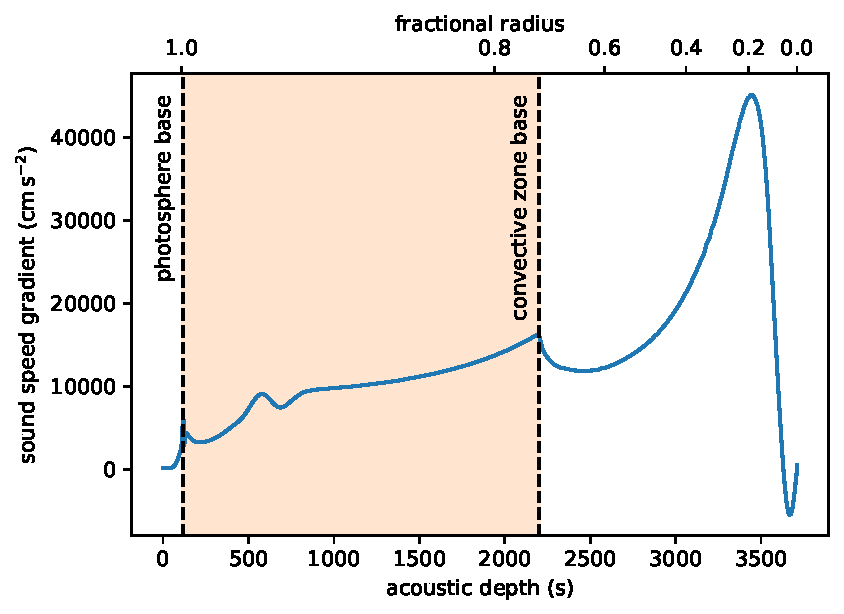
\includegraphics{figures/sound-speed-gradient.pdf}
    \caption{The sound speed gradient (\(\dd c/\dd \tau\)) of model S plot against the acoustic depth (\(\tau\)). The fractional radius to the photosphere base is given on the top axis. The convective envelope is shaded and the bases of the photosphere and convective zone are marked with dashed lines.}
    \label{fig:sound-speed-gradient}
\end{figure}

In Figure \ref{fig:sound-speed-gradient}, we show the sound speed gradient with respect to \(\tau\) for a Sun-like stellar model (model S; see Section \ref{sec:model-s}). We see how the speed of sound changes smoothly throughout the star. In the convective envelope, where p-modes propagate, there is a noticeable wiggle around \SI{700}{\second} and a sharp change in direction at its base. The first is caused by the ionisation of helium, which we will explore further in Section \ref{sec:helium-glitch}. The second is due to a discontinuity in the second temperature gradient as the stellar interior goes from convectively unstable to radiative. This will be discussed in Section \ref{sec:bcz-glitch}.

\subsection{Sun-Like Model Star}\label{sec:model-s}

We computed a representative Sun-like model star (hereafter model S) using MESA \citep[version 12115;][]{Paxton.Bildsten.ea2011,Paxton.Cantiello.ea2013,Paxton.Marchant.ea2015,Paxton.Schwab.ea2018,Paxton.Smolec.ea2019,Jermyn.Bauer.ea2023}. The model was computed with an initial mass of \SI{1.0}{\solarmass} to a central fractional hydrogen abundance of 0.6. We used initial fractional helium and heavy-element abundances of 0.28 and 0.02 respectively. The mixing-length was parameterised by \(\alpha_\mlt=1.9\) and a turbulent pressure factor of 1. We evolved the star using element diffusion with MESA's default coefficients \citep{Stanton.Murillo2016}. In addition, we used MESA's default \citet{Grevesse.Sauval1998} solar chemical composition and opacity tables.We also output pulsation profile data in FGONG format to later use when computing oscillation modes in Chapter \ref{chap:glitch-gp}. Our resulting model S had an age of \SI{4.073}{\giga\year}, \(\teff \approx \SI{5682}{\kelvin}\), and \(R \approx \SI{1.014}{\solarradius}\). Since the model was evolved with element diffusion, the surface fractional helium and heavy-element were approximately \num{0.2515} and \num{0.01810} respectively.

\subsection{Helium Ionisation Glitch}\label{sec:helium-glitch}

In this section, we will first show how the sound speed inside a solar-like star is affected by the ionisation of hydrogen and helium. Then, we will see that an increase in helium abundance (\(Y\)) increases the effect of helium ionisation on the speed of sound. Starting with the variational principle, we derive a commonly used form of the glitch signature found in the mode frequencies. In the process, we show that the p modes are sensitive to rapid changes in sound speed near the surface.

\subsubsection{The Effect of Helium Abundance on \(\gamma\)}

In the outer convective envelope of Sun-like stars, the temperature (\(\SIrange{e4}{e5}{\kelvin}\)) and density (\(\SIrange{e-5}{e-3}{\gram\per\centi\metre\cubed}\)) is suitable for ionising hydrogen and helium \citep{Eggleton.Faulkner.ea1973}. As a given chemical species in the star ionises, the number of particles and hence chemical potential of the species changes. This induces a gradient in the thermal free energy of the gas which relates to the pressure and entropy of the gas. Thus, we expect ionisation to cause a change in the pressure-density gradient at constant entropy, \(\gamma\). Since \(\gamma\) relates to the sound speed from Equation \ref{eq:sound}, any sudden change in \(\gamma\) will induce a change in \(c\).

\begin{figure}[tb]
    \centering
    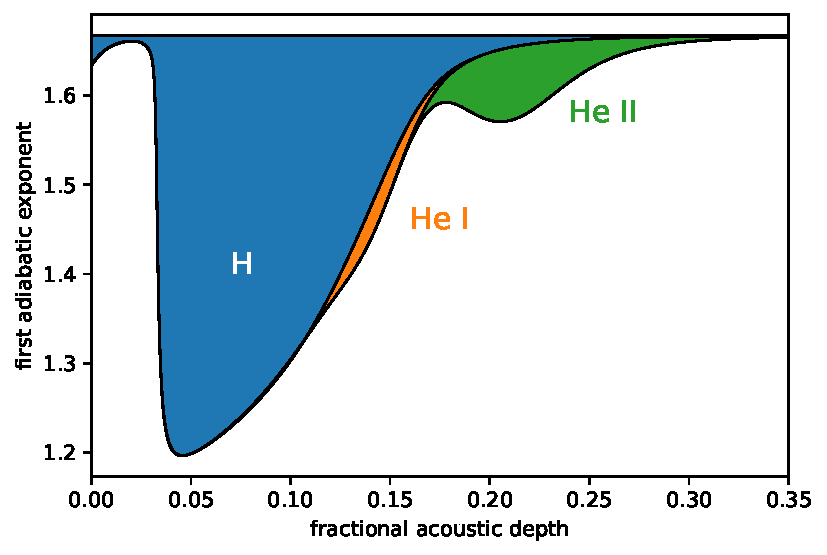
\includegraphics{figures/adiabatic-ionisation-regions.pdf}
    \caption[The depressions in the first adiabatic exponent caused by the ionisation of hydrogen and helium.]{The depressions in the first adiabatic exponent (\(\gamma\)) caused by the ionisation of hydrogen (H), and the first and second ionisations of helium (He\,\textsc{i} and He\,\textsc{ii}). The horizonal axis is the fractional acoustic depth from the surface of the star, \(\tau/\tau_0\).}
    \label{fig:gamma-zones}
\end{figure}

In Figure \ref{fig:gamma-zones}, we show \(\gamma\) for model S against fractional acoustic depth, shaded by regions of ionisation. For an ideal monatmoic gas, \(\gamma=5/3\), but \(\gamma < 5/3\) in regions where helium and hydrogen ionise. Close to the surface of the star, hydrogen ionisation has the largest effect on \(\gamma\) because it makes up the majority of stellar matter. The first (He\,\textsc{i}) and second (He\,\textsc{ii}) ionisations of helium occur deeper in the star. We can see that the second ionisation of helium has a greater affect on \(\gamma\) than the first. The effect of the second He ionisation causes a rapid changing in \(\gamma\) over a few per cent in \(\tau\) (equivalent to \(\sim \SI{50}{\second}\) in model S).

\begin{figure}
    \centering
    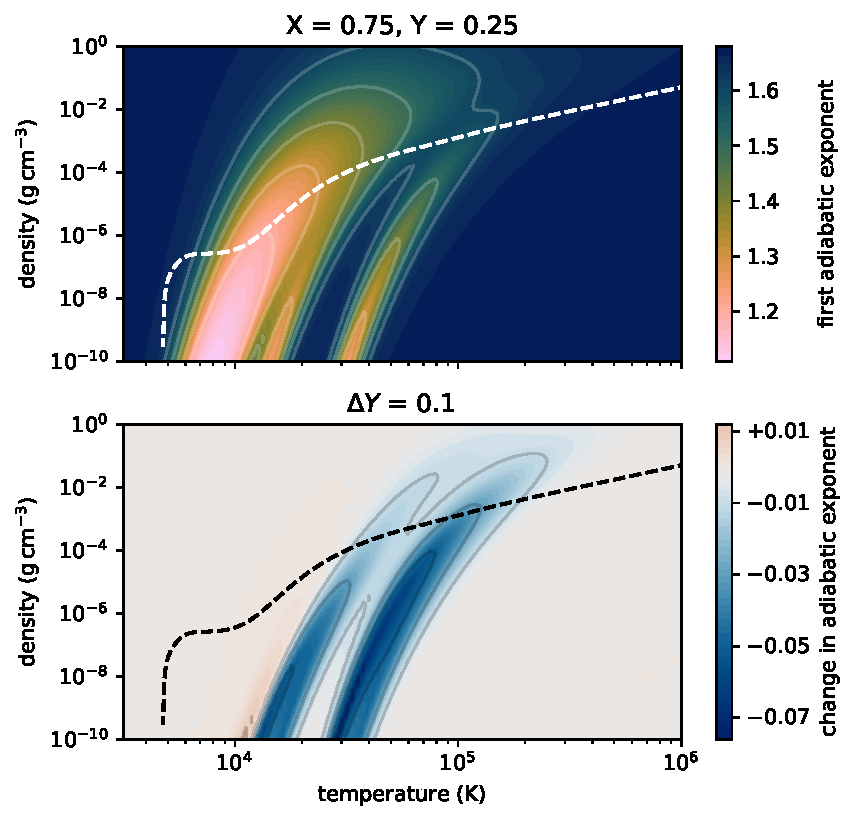
\includegraphics{figures/adiabatic-ionisation-temp.pdf}
    \caption[Temperature-density profile for a Sun-like star.]{Temperature-density profile for a Sun-like star. \emph{Top:} The first adiabatic exponent \(\gamma\) as a function of temperature and density, calculated using Eq. 53 of \citet{Houdayer.Reese.ea2021} for a helium mass fraction, \(Y=0.25\). \emph{Bottom:} The change in \(\gamma\) induced by a change in helium abundance, \(\Delta Y = 0.1\). In both panels, the dashed line shows the temperature-density profile of model S.\\--- \emph{This figure is a recreation of Fig. 5 in \citet{Houdayer.Reese.ea2021}.}}
    \label{fig:gamma-temp-density}
\end{figure}

We were able to isolate the contributions to \(\gamma\) from ionisation using a recent derivation by \citet{Houdayer.Reese.ea2021}. They obtained an approximate formula for \(\gamma\) as a function of temperature (\(T\)) and density valid for the outer convective zone of Sun-like stars. Using their formula, we plot \(\gamma\) for a range of \(T\) and \(\rho\) in Figure \ref{fig:gamma-temp-density}. The first panel illustrates the three ionisation regions of hydrogen and helium. The value of \(\gamma\) decreases when the ionisation reaction is occurring. The magnitude of this effect depends on the temperature-density profile of the star which we can see over-plot for model S. We can imagine a hotter star shifting this line such that ionisation occurs closer to the surface. In the second panel, we see that an increase in helium abundance by 0.1 decreases \(\gamma\) by up to \(\sim 0.03\) in the He\,\textsc{ii} ionisation region along the model S profile. This shows that helium abundance correlates with the size of the glitch in \(\gamma\). However, there is clearly still some dependence on other stellar quantities.

% The exact effect of ionisation on \(\gamma\) is not known analytically. However, \citet{Houdayer.Reese.ea2021} recently approximated \(\gamma\) for the convective zone of a Sun-like star in their study of the helium ionisation glitch. In this subsection, we combine the equations derived in their work to help us understand the relation between ionisation and \(\gamma\). Let us consider an \(M\) mass star with fractional hydrogen and helium abundances of \(X\) and \(Y\) respectively. From \citet{Houdayer.Reese.ea2021}, we approximate the first adiabatic exponent as,
% %
% \begin{equation}
%     \gamma \simeq \frac{5}{3} - \frac{2}{3} \, \eta(T, \rho), \label{eq:gamma1}
% \end{equation}
% %
% where \(\eta\) represents the depression in \(\gamma\). Considering a hydrogen-helium mixture where \(X + Y \approx 1\), \(\eta\) is,
% %
% \begin{equation}
%     \begin{split}
%         \eta(T, \rho) &= \frac{1}{\partial_{TT}^2 f} \left[n_\hydrogen y_\hydrogen \, (1 - y_\hydrogen) \, \frac{(\chi_\hydrogen / k_B T)^2}{2 - y_\hydrogen}
%         % \right. \\ &\left. 
%         + n_\helium y_\helium^{(1)} \left(1 - y_\helium^{(1)}\right) \left(\frac{\chi_\helium^{(1)}}{k_B T}\right)^2 
%         \right. \\ &\left.
%         + \, n_\helium y_\helium^{(2)} \left(1 - y_\helium^{(2)}\right) \left(\frac{\chi_\helium^{(2)}}{k_B T}\right)^2\right],
%     \end{split}
% \end{equation}
% %
% where \(k_B\) is the Boltzmann constant. The parameter \(\partial_{TT}^2\) is the second partial derivative of the free energy density with respect to temperature (\(T\)),
% %
% \begin{equation}
%     \begin{split}
%         \partial_{TT}^2 f &\simeq \frac{3}{2} + n_\hydrogen y_\hydrogen \left[ \frac{3}{2} + \frac{(1 - y_\hydrogen)}{2 - y_\hydrogen} \left(\frac{3}{2} + \frac{\chi_\hydrogen}{k_B T}\right)^2 \right] %\\
%         + n_\helium y_\helium^{(1)} \left[ \frac{3}{2} + \left(1 - y_\helium^{(1)}\right) \left(\frac{3}{2} + \frac{\chi_\helium^{(1)}}{k_B T}\right)^2 \right] \\
%         &+ n_\helium y_\helium^{(2)} \left[ \frac{3}{2} + \left(1 - y_\helium^{(2)}\right) \left(\frac{3}{2} + \frac{\chi_\helium^{(2)}}{k_B T}\right)^2 \right],
%     \end{split}
% \end{equation}
% %
% where \(n_\mathbb{X} = N_\mathbb{X} / N\) is the number density and \(\chi_\mathbb{X}^{i}\) is the \(i\)-th ionisation energy of species \(\mathbb{X}\). Parameter \(y_\mathbb{X}^i\) is related to a reduced form of Saha's equation \needcite,
% %
% \begin{equation}
%     \frac{(y_\mathbb{X}^i)^q}{1 - y_\mathbb{X}^i} = \frac{2 g_\mathbb{X}^i}{g_\mathbb{X}^{i-1}} \frac{\overline{m}}{\rho \lambda_\ee^3} \, \ee^{- \chi_\mathbb{X}^i / k_B T},
% \end{equation}
% %
% where \(q = 2\) for hydrogen, \(q = 1\) for helium, \(\overline{m} = M/N\) is the mean mass, and \(g_\mathbb{X}^i\) is the ground-state degeneracy of ionisation state \(i\). We used these equations to produce Figures \ref{fig:gamma-zones} and \ref{fig:gamma-temp-density}.

\subsubsection{The Effect of \(\gamma\) on p Mode Frequencies}

\begin{figure}
    \centering
    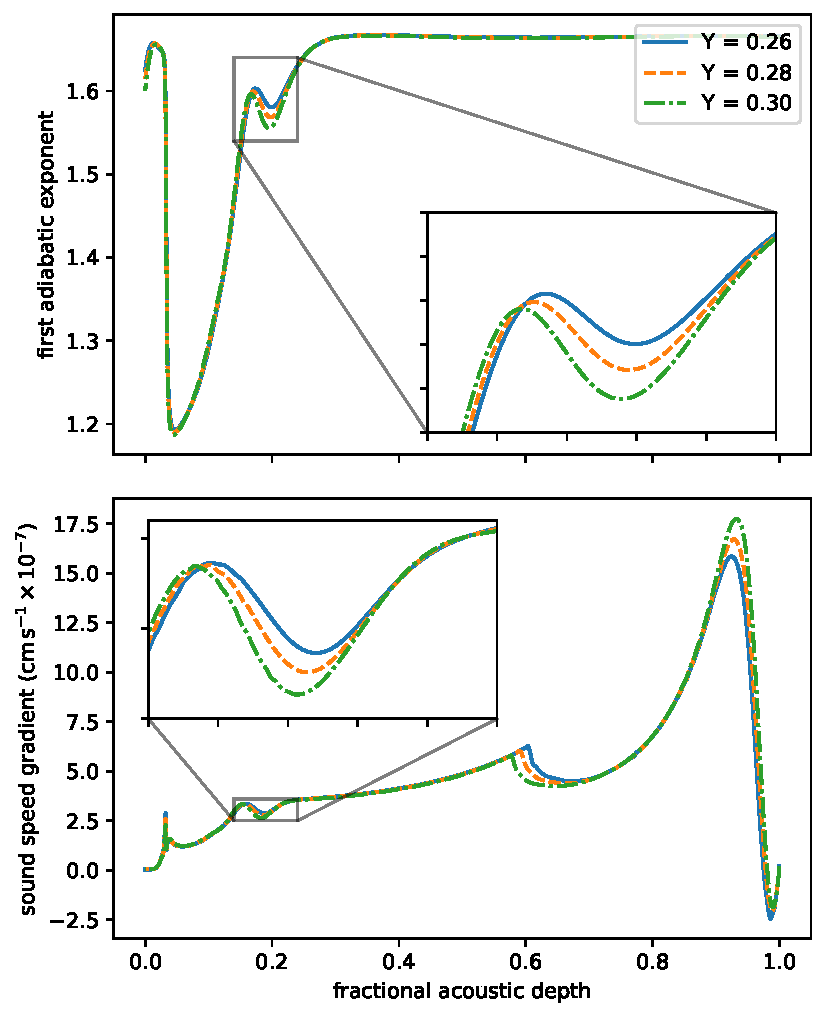
\includegraphics{figures/helium-ionisation-sound-speed.pdf}
    \caption{The effect on the sound speed profile for three solar-like stars with initial helium mass fractions of 0.26 (\emph{solid}), 0.28 (\emph{dashed}), and 0.3 (\emph{dot-dashed}). The models were each evolved to a central helium mass fraction of 0.6. \emph{Top:} The first adiabatic exponent \(\gamma\). \emph{Bottom:} The sound speed gradient \(\dd c/\dd t\) where \(t = \tau/\tau_0\) is the fractional acoustic depth.}
    \label{fig:gamma-sound-speed}
\end{figure}

To show the effect of small changes in \(Y\) on the sound speed, we plot the sound speed gradient in Figure \ref{fig:gamma-sound-speed}. The three models shown were evolved to the same central temperature as model S with initial helium abundances of 0.26, 0.28, and, 0.3. The dominant effect of helium abundance appears as a Gaussian-like depression in \(\gamma\) around the second ionisation of helium. We see how larger helium abundance increases the width and depression in \(\gamma\), which is reflected in the sound speed gradient. A larger \(Y\) also leads to a relative reduction in hydrogen abundance (\(X\)) which shrinks the width of the hydrogen ionisation region.

To see how a change in \(\gamma\) affects the mode frequencies, we explore the sensitivity of a mode to rapid structural changes in the star. Starting with the variational principle, we can approximate the characteristic frequencies of a spherically symmetric, slowly rotating star by \citep{Chandrasekhar1964},
%
\begin{equation}
    \omega^2 = \frac{\mathcal{E}}{\mathcal{I}}\label{eq:var-prin}
\end{equation}
%
which is a ratio of \(\mathcal{E}\) (proportional to the mode's energy)
%
% \begin{equation}
%     \mathcal{E} = \int_0^R \left[\gamma P (\dive{\vect{\xi}})^2 + 2(\vect{\xi}\cdot \nabla P) \dive{\vect{\xi}} + (\vect{\xi}\cdot \nabla P) (\vect{\xi}\cdot\nabla\ln\rho)\right] r^2 \, \dd r.
% \end{equation}
%
to its inertia (\(\mathcal{E}\)). The mode inertia is,
%
\begin{equation}
    \mathcal{I} = \int_0^R \vect{\xi} \cdot \vect{\xi} \, \rho r^2 \, \dd r.
\end{equation}
%
where the amplitude and direction of a pressure wave at a given point in a star is given by the so-called Lagrangian perturbation vector \(\vect{\xi}\). 

\begin{figure}
    \centering
    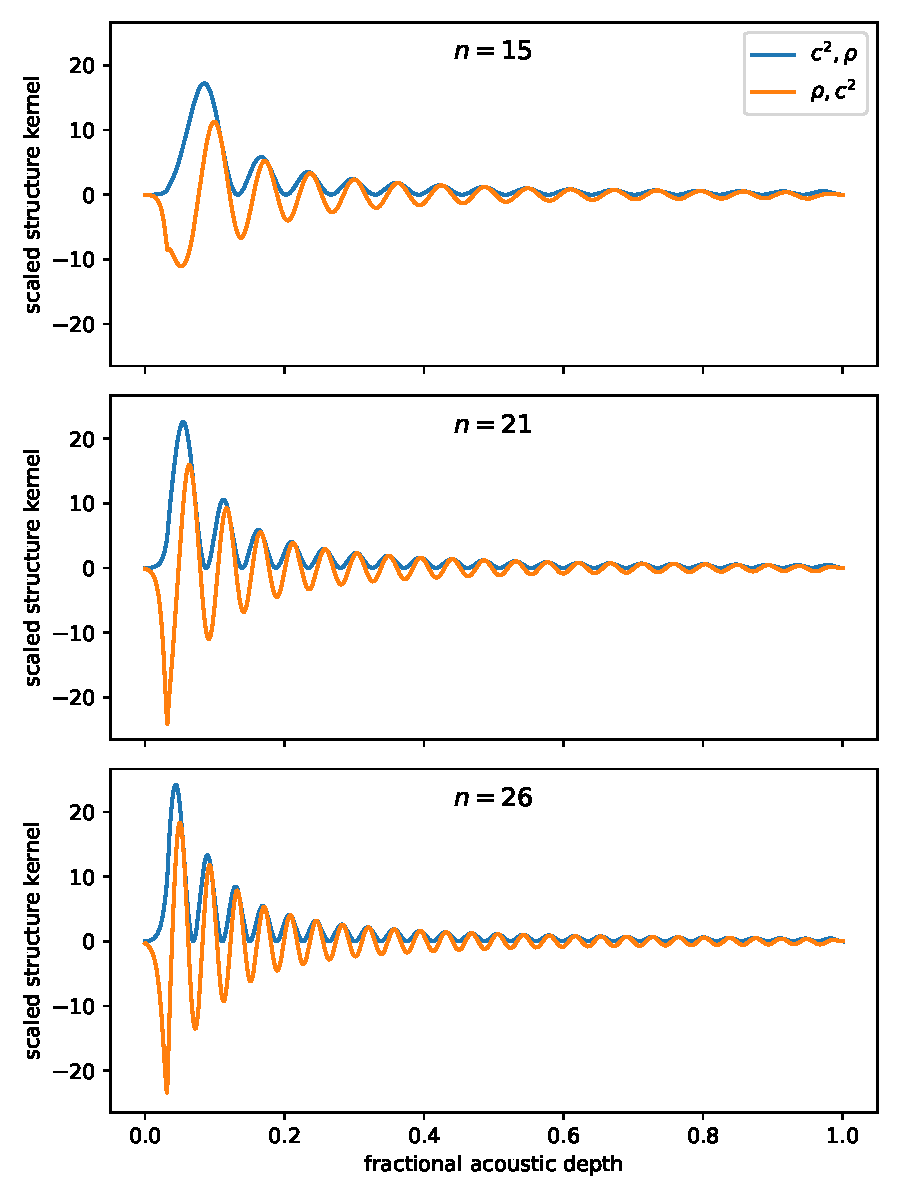
\includegraphics{figures/kernels.pdf}
    \caption{Structure kernels (\(\mathcal{K}_{c^2,\rho}, \mathcal{K}_{\rho,c^2}\)) scaled by the stellar radius as a function of fractional acoustic depth. The kernels were computed for three radial oscillation modes (\(n=15,21,26\)) using oscillation calculations for stellar model S.}
    \label{fig:kernels}
\end{figure}

A structural glitch in the star would cause a small change in frequency (\(\delta\omega\)). Differentiating both sides of Equation \ref{eq:var-prin} with respect to \(\omega\), we get,
%
\begin{align}
    2\omega &= \frac{1}{\mathcal{I}} \left( \frac{\delta\mathcal{E}}{\delta\omega} - \omega^2 \frac{\delta\mathcal{I}}{\delta\omega}\right), \qquad \left[\times \frac{\delta\omega}{2\omega^2}\right] \notag \\
    \frac{\delta\omega}{\omega} &= \frac{1}{2\,\mathcal{I}} \left(\frac{\delta\mathcal{E}}{\omega^2} - \delta\mathcal{I}\right).
\end{align}
%
Small changes \(\delta\mathcal{E}\) and \(\delta\mathcal{I}\) depend on changes to the state variables. By perturbing and substituting appropriate forms of \(\mathcal{E}\) and \(\mathcal{I}\), it is possible to rewrite this as a function of the so-called structural kernels \(\mathcal{K}_{a,b}\). For example \citep{Christensen-Dalsgaard2014},
%
\begin{equation}
    \frac{\delta\omega}{\omega} = \int_0^R \left(\mathcal{K}_{c^2,\rho} \frac{\delta c^2}{c^2} + \mathcal{K}_{\rho,c^2} \frac{\delta \rho}{\rho} \right) \dd r.\label{eq:kernels}
\end{equation}
%
where \(\mathcal{K}_{a, b}\) gives the relative effect on \(\omega\) due to a perturbation in a state variable \(a\) at fixed \(b\), at a given \(r\). The kernels, defined fully in \citet{Gough.Thompson1991}, can show the sensitivity of the wave to a change in state in the star. We plot \(\mathcal{K}_{c^2,\rho}\) and \(\mathcal{K}_{\rho,c^2}\) in Figure \ref{fig:kernels} for a few radial oscillation modes. Both decay through the star, meaning that the modes are less sensitive to structural changes deeper in the star. The kernels also oscillate at different frequencies, meaning that some modes will be more or less sensitive to a glitch than others.

We can evaluate Equation \ref{eq:kernels} to find the effect on \(\omega\) due to a change in \(\gamma\) from helium ionisation. The first term can be easily rewritten in terms of a change in \(\gamma\) because \(c^2 \propto \gamma\), hence \(\mathcal{K}_{\gamma,\rho} \delta \gamma / \gamma \equiv \mathcal{K}_{c^2,\rho} \delta c^2 / c^2\). Helium ionisation has a negligible effect on density, so we can assume \(\delta\rho/\rho \approx 0\) in the ionisation region. Therefore, we may rewrite Equation \ref{eq:kernels} due to a change in \(\gamma\) as,
%
\begin{equation}
    \left.\frac{\delta\omega}{\omega}\right|_\gamma \simeq \int_0^R \mathcal{K}_{\gamma,\rho} \frac{\delta\gamma}{\gamma} \dd r,\label{eq:delta-omega}
\end{equation}
%
where \(\mathcal{K}_{\gamma,\rho}\) is shown in \citet{Gough1993} to satisfy,
%
\begin{equation}
    \omega^2 \mathcal{I}\mathcal{K}_{\gamma,\rho} = \frac12 \gamma P (\dive{\vect{\xi}})^2 r^2.\label{eq:gamma-kernel}
\end{equation}
%

Firstly, we expand the mode inertia, \(\mathcal{I}\). The Lagrangian perturbation vector can be written in terms of a radial and horizontal component, \(\vect{\xi} = \xi_r \hat{r} + \vect{\xi}_h\). In the high-order limit where \(l/n \rightarrow 0\), the horizontal component \(\vect{\xi}_h\) is negligible. Therefore, we can rewrite the mode inertia as,
%
\begin{equation}
    \mathcal{I} \simeq \int_0^R \xi_r^2 \rho r^2 \, \dd r.
\end{equation}
%
Then, we use an approximation of \(\xi_r\) from \citet{Gough1993}, 
%
\begin{equation}
    \xi_r \simeq \frac{\psi_0}{r}\sqrt{\frac{K}{\rho}} \cos\psi,\label{eq:xi-r}
\end{equation}
%
where \(\psi_0\) is a proportionality constant and the radial wave number \(K \simeq \omega / c\) for high-order acoustic modes. The phase term \(\psi \simeq \omega \tau + \epsilon\) when \(\tau\) is not close to the upper turning point (where the wave is reflected near the stellar surface). The small offset \(\epsilon\) is a slowly varying function of \(\tau\). Substituting Equation \ref{eq:xi-r} into the mode inertia gives,
%
\begin{align}
    \mathcal{I} &\simeq \psi_0^2 \int_0^R K \cos^2\psi \, \dd r \notag \\
    &= \frac12 \omega \psi_0^2 \int_0^R (1 + \cos 2 \psi) \frac{\dd r}{c}.
\end{align}
%
Finally, changing to an integral over the acoustic depth, \(\tau\) we can evaluate the integral for high-order modes where \(\omega_n \ll \tau_0^{\,-1}\),
%
\begin{equation}
    \mathcal{I} \simeq \frac12 \omega \psi_0^2 \int_0^{\tau_0} [1 + \cos 2 (\omega\tau + \epsilon)] \, \dd \tau \simeq \frac12 \omega \psi_0^2 \tau_0.
\end{equation}
%

Secondly, we substitute an approximation for \((\dive{\vect{\xi}})^2\) from \citet{Gough1993},
%
\begin{equation}
    (\dive{\vect{\xi}})^2 \simeq \frac{\psi_0^2 \omega^3}{\gamma P c r^2} \sin^2\psi, \label{eq:div-xi}
\end{equation}
%
into Equation \ref{gamma-kernel} to get,
%
\begin{align}
    \left.\frac{\delta\omega}{\omega}\right|_\gamma &\simeq \frac{1}{2\omega^2\mathcal{I}} \int_0^{R} \delta\gamma P (\dive{\vect{\xi}})^2 r^2 \, \dd r, \notag \\
    &\simeq \frac{\omega \psi_0^2}{2 \mathcal{I}} \int_0^{R} \frac{\delta\gamma}{\gamma}\sin^2\psi\frac{\dd r}{c}, \notag \\
    &= \frac{\omega \psi_0^2}{4 \mathcal{I}} \int_0^{R} \frac{\delta\gamma}{\gamma}(1 - \cos 2\psi)\frac{\dd r}{c}.
\end{align}
%
We can see that \(\delta\omega\) is split into a smooth and a periodic component. The smooth component may be treated later, but for now we focus on the oscillating part of \(\delta\omega\). Substituting for \(\mathcal{I}\) and \(\psi\), changing to an integral over acoustic depth we get,
%
\begin{equation}
    \left.\frac{\delta\omega}{\omega}\right|_{\gamma,\mathrm{osc}} \simeq - \frac{1}{2\tau_0} \int_0^{\tau_0} \frac{\delta\gamma}{\gamma} \cos 2 (\omega\tau + \epsilon) \, \dd \tau. \label{eq:omega-osc}
\end{equation}
%

\subsubsection{A Functional Form of the Helium Glitch Signature}

We have shown that a change in \(\gamma\) can induce a periodicity in \(\omega\). The functional from of this periodicity depends on \(\delta\gamma/\gamma\). As shown in Figures \ref{fig:gamma-zones} and \ref{fig:gamma-temp-density}, the dominant perturbation due to a change in helium abundance is from the second ionisation of helium. There have been different attempts to approximate \(\delta\gamma/\gamma\,|_\heII\) in the literature, for example using a Dirac delta function or a triangular function \citep{Monteiro.Christensen-Dalsgaard.ea1994, Monteiro.Thompson2005}. In recent years, work modelling the glitch has used the formulation from \citet{Houdek.Gough2007} where the change in \(\gamma\) due to He\,\textsc{ii} ionisation is modelled with a Gaussian shape,
%
\begin{equation}
    \left.\frac{\delta\gamma}{\gamma}\right|_\heII \simeq - \frac{\Gamma_\heII}{\Delta_\heII \sqrt{2\pi}} \, \ee^{- \frac12{(\tau - \tau_\heII)^2}/{\Delta_\heII^2} }, \label{eq:he-gamma}
\end{equation}
%
where \(\Gamma_\heII\) is the area, \(\Delta_\heII\) is the characteristic width, and \(\tau_\heII\) is the center of the ionisation region.

Here, we independetly verify result for \(\delta\omega\) due to He\,\textsc{ii} ionisation from \citet{Houdek.Gough2007}. Substituting Equation \ref{eq:he-gamma} into Equation \ref{eq:omega-osc} with a change of variables to \(x = (\tau - \tau_\heII)/\Delta_\heII\), we get,
%
\begin{equation}
    \left.\frac{\delta\omega}{\omega}\right|_{\heII, \mathrm{osc}} \simeq \frac{\Gamma_\heII}{2\sqrt{2\pi} \, \tau_0} \, \int_{-\infty}^\infty \ee^{- x^2/2} \cos 2 (\Delta_\heII \omega x + \widetilde{\epsilon_\heII}) \, \dd x \label{eq:omega-ii-osc}
\end{equation}
%
where \(\widetilde{\epsilon_\heII} = \omega\tau_\heII + \epsilon_\heII\) and the phase \(\epsilon=\epsilon_\heII\) is assumed constant accross the glitch region. We can solve the above integral analytically using differentiation under the integral sign by introducing an arbitrary variable \(a\),
%
\begin{equation}
    I(a) = \int_{-\infty}^\infty \ee^{- x^2/2 } \cos 2 (\Delta_\heII \omega x a + \widetilde{\epsilon_\heII}) \, \dd x
\end{equation}
%
Differentiating this with respect to \(a\), and then integrating by parts gets,
%
\begin{align}
    I'(a) &= - 2 \Delta_\heII \omega \int_{-\infty}^\infty x \, \ee^{- x^2/2 } \sin 2 (\Delta_\heII \omega x a + \widetilde{\epsilon_\heII}) \, \dd x, \notag\\
    &= - 2 \Delta_\heII \omega \int_{-\infty}^\infty \sin 2 (\Delta_\heII \omega x a + \widetilde{\epsilon_\heII}) \, \dd \ee^{- x^2/2 }, \notag\\
    &= 2 \Delta_\heII \omega \left\{ \left[ \ee^{- x^2/2 } \sin 2 (\Delta_\heII \omega x a + \widetilde{\epsilon_\heII}) \right]_{-\infty}^\infty - 2 \Delta_\heII \omega a \int_{-\infty}^\infty \ee^{- x^2/2 } \cos 2 (\Delta_\heII \omega x a + \widetilde{\epsilon_\heII}) \, \dd x \right\}, \notag\\
    &= - 4 \Delta_\heII^2 \omega^2 a \, I(a),
\end{align}
%
which is a differential equation with the solution,
%
\begin{equation}
    \begin{split}
        I(a) = I(0) \ee^{- 2 \Delta_\heII^2 \omega^2 a^2}, \qquad I(0) &= \int_{-\infty}^\infty \ee^{- x^2/2 } \cos 2 \widetilde{\epsilon_\heII} \, \dd x, \\
        &= \sqrt{2\pi} \, \cos 2 \widetilde{\epsilon_\heII},
    \end{split}
\end{equation}
%
Therefore, if we set \(a = 1\) (to get back to the integral in Equation \ref{eq:omega-ii-osc}) we get the following for the periodic glitch signature \citep[cf.][Eq. 15]{Houdek.Gough2007},
%
\begin{equation}
    \left.\frac{\delta\omega}{\omega}\right|_{\heII, \mathrm{osc}} \simeq \frac{\Gamma_\heII}{2 \tau_0} \ee^{- 2 \Delta_\heII^2 \omega^2} \cos 2 (\tau_\heII\omega + \epsilon_\heII),
\end{equation}
%
We can rearrange this to a more familiar form in terms of cyclic frequency \citep[e.g.][]{Verma.Faria.ea2014,Verma.Raodeo.ea2017}, by substituting \(\omega = 2\pi\nu\),
%
\begin{equation}
    \left.\frac{\delta\nu}{\nu}\right|_{\heII, \mathrm{osc}} \simeq \nu_0 \Gamma_\heII \, \ee^{- 8 \pi^2 \Delta_\heII^2 \nu^2} \, \sin ( 4 \pi \tau_\heII \nu + \phi_\heII), \label{eq:he-osc}
\end{equation}
%
where \(\phi_\heII = 2(\epsilon_\heII + \pi/4)\), and \(\nu_0 = (2 \tau_0)^{-1}\) is the inverse acoustic diameter of the star.

\subsection{Base of the Convective Zone Glitch}\label{sec:bcz-glitch}

\begin{figure}[tb]
    \centering
    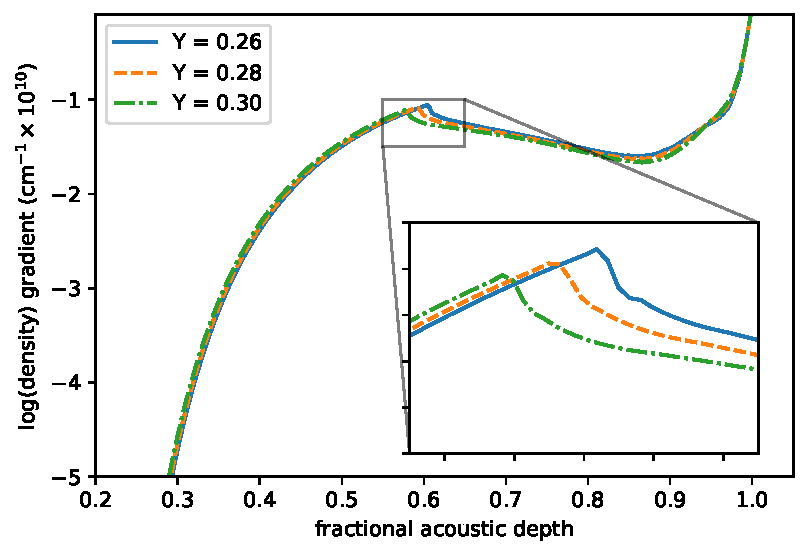
\includegraphics{figures/bcz-density-gradient.pdf}
    \caption{Discontinuity in the density gradient at the base of the convective zone for three solar-like stars with initial helium mass fractions of 0.26 (\emph{solid}), 0.28 (\emph{dashed}), and 0.3 (\emph{dot-dashed}).}
    \label{fig:bcz-density}
\end{figure}

The sensitivity of p-modes to glitches gets smaller further into the star. However, we should not neglect the effect of the near-discontinuity at the base of the convective zone (BCZ). This arises from a jump in the second derivative of temperature at the BCZ which translated to discontinuities in the second derivative of density and sound speed. In Figure \ref{fig:bcz-density} we can see a fast change in direction of the density gradient around \(\tau/\tau_0 \approx 0.6\) (or at about \SI{2200}{\second} for model S). We also see that the relative location of the BCZ changes a little with \(Y\).

% Overshoot actually causes discontinuity in first derivative, not second \citep{Zahn1991}.

We could take a similar approach to the previous section but now considering the second kernel \(\mathcal{K}_{\rho,c^2}\) in Equation \ref{eq:kernels} since the discontinuity affects \(\rho\). However, \citet{Houdek.Gough2007} take another approach by considering the discontinuity as it appears in the acoustic cut-off frequency, \(\omega_{ac}\). The details of this derivation are beyond the scope of this work. Instead, we quote their result for the change in frequency induced by a density discontinuity at the base of the convective zone located at an acoustic depth of \(\tau_\bcz\) \citep[cf.][Eq. 17]{Houdek.Gough2007},
%
\begin{equation}
    \left.\frac{\delta\omega}{\omega}\right|_{\bcz,\mathrm{osc}} \simeq \frac{c_\bcz^2\Delta_\bcz}{8\tau_0 \omega^3} \left(1 + {1}/{4\tau_0^2\omega^2}\right)^{-1/2} \cos\left[2(\tau_\bcz \omega + \epsilon_\bcz) + \tan^{-1}(2\tau_0\omega)\right]
\end{equation}
%
where \(\epsilon_\bcz\) is some phase which depends slowly on \(\omega\), \(c_\bcz\) is the speed of sound and,
%
\begin{equation}
    \Delta_\bcz = \left[\frac{\dd^2 \ln\rho}{\dd r^2}\right]_{-r_\bcz}^{+r_\bcz},
\end{equation}
%
is the change in second derivative of density at the base of the convective zone (\(r = r_\bcz\)).

For high-order modes, \(\tau_0 \omega \gg 1\) and thus \(\tan^{-1}(2\tau_0\omega) \simeq \pi/2\), and \((1 + {1}/{4\tau_0^2\omega^2})^{-1/2} \simeq 1\). Therefore, we can simplify this and write it in a more familiar form in terms of cyclic frequency,
%
\begin{equation}
    \left.\frac{\delta\nu}{\nu}\right|_{\bcz,\mathrm{osc}} \simeq \frac{c_\bcz^2\Delta_\bcz}{32\pi^3}\frac{\nu_0}{\nu^3} \sin(4\pi\tau_\bcz\nu + \phi_\bcz) \label{eq:bcz-osc}
\end{equation}
%
where \(\phi_\bcz\) is some approximately constant phase term.

Now we have equations for the effect of He\,\textsc{ii} ionisation and the BCZ for a given mode frequency \(\nu\), we can use them to model the glitch signatures as they appear in observed mode frequencies, \(\nu_{nl}\). Naturally, these equations are not exact. Several assumptions were made during their derivations. Therefore, if we want to model the glitch signature in \(\nu_{nl}\), we need some way of accounting for the uncertainty in the above equations. In the next chapter, we apply this model to characterise the glitch for a test star and real star. Although such models have been applied to other Sun-like stars before \citep[e.g.][]{Mazumdar.Monteiro.ea2014,Verma.Faria.ea2014}, we propose a new statistical model which uses a Gaussin process to account for the uncertainty in the functional form of \(\nu_{nl}\).

  % chapters/glitch-gp.tex
%
% Copyright 2023 Alexander Lyttle.
%
% This work may be distributed and/or modified under the conditions of the
% LaTeX Project Public License (LPPL) version 1.3 or later.
%
% The latest version of this license is in
% https://www.latex-project.org/lppl.txt and version 1.3 or later is part of
% all distributions of LaTeX version 2005/12/01 or later.
%
%
\chapter[Modelling Acoustic Glitches with a Gaussian Process]{Modelling Acoustic Glitch Signatures in Stellar Oscillations with a Gaussian Process}\label{chap:glitch-gp}

\textit{In this chapter, I apply a new method for modelling acoustic glitch signatures in the radial mode frequencies of solar-like oscillators. I compare my method to another using a model star with different levels of noise. Then, I apply both methods to the star 16 Cyg A. I show that my method can be used to find the strength and location of glitches caused by the second ionisation of helium and the base of the convective zone. I also demonstrate that my method improves treatment of the smoothly varying component of the mode frequencies.}

\section{Introduction}

Let us consider a non-rotating star which oscillates at frequencies \(\nu_{nl}\), where \(n\) and \(l\) are the radial order and angular degree of the modes. We may model the modes as the sum of a smoothly-varying component, \(\tilde{f}(n, l)\), and quickly-varying, small change in frequency, \(\delta\nu\), arising from glitches in the stellar structure,
%
\begin{equation}
    f(n, l) = \tilde{f}(n, l) + \delta\nu,\label{eq:general-glitch}
\end{equation}
%
where \(\delta\nu\) is some function of frequency which may be evaluated at \(\tilde{f}(n, l)\).

In principle, \(\delta\nu\) could arise from any glitches expected in a particular star. Here, we consider glitches in main sequence solar-like oscillators. In Chapter \ref{chap:glitch}, we derived approximations for \(\delta\nu\) arising from acoustic glitches caused by the second ionisation of helium and the BCZ. We choose to ignore contributions to \(\delta\nu\) from the first ionisation of helium. Consequently, we let \(\delta\nu = \delta\nu_\helium + \delta\nu_\bcz\) where each component depends on parameters relating to properties of the glitches (cf. Equations \ref{eq:he-osc} and \ref{eq:bcz-osc}),
%
\begin{align}
    \delta\nu_\helium &= \alpha_\helium \nu_0 \nu \, \ee^{-\beta_\helium \nu^2} \sin(4\pi\tau_\helium\nu + \phi_\helium), \label{eq:he-glitch}\\
    \delta\nu_\bcz &= \alpha_\bcz \nu_0 \nu^{-2} \, \sin(4\pi\tau_\bcz\nu + \phi_\bcz). \label{eq:bcz-glitch}
\end{align}
%
The parameters \(\alpha_\helium \simeq \Gamma_\heII\) and \(\beta_\helium \propto \Delta_\heII^2\) relate to the area and variance of the Gaussian-like depression in \(\gamma\) caused by the second ionisation of helium (see Equation \ref{eq:he-gamma}). The amplitude parameter for the BCZ glitch is proportional to the difference in the second density derivative at the base of the convective zone (\(\alpha_\bcz \propto \Delta_{\bcz}\)) with units of frequency squared. The approximate acoustic depths of second helium ionisation and the BCZ are given by \(\tau_\helium\) and \(\tau_\bcz\) respectively, and \(\phi_\helium\) and \(\phi_\bcz\) are arbitrary phase constants.

Providing \(\tilde{f}(n, l)\) is a good approximation of the mode frequencies, we can calculate \(\delta\nu\) at \(\nu = \tilde{f}(n, l)\) to predict \(f(n, l)\). For example, \(\tilde{f}(n,l)\) could be a \(K\)-th order polynomial in \(n\) with coefficients \(a_{lk}\) \citep[e.g.][]{Kjeldsen.Bedding.ea2005,Ulrich1986},
%
\begin{equation}
    \tilde{f}(n, l) = \nu_0 \sum_{k=0}^{K} a_{lk} n^k. \label{eq:poly}
\end{equation}
%
The linear component of this is equivalent to the asymptotic expression (see Equation \ref{eq:asy}) and the remaining terms describe curvature in the mode frequencies. However, there are drawbacks to using a polynomial for \(\tilde{f}(n, l)\). Whilst a polynomial with \(K = \infty\) can represent any function, this is impractical here. If \(K\) is too low, then it will not be flexible enough, biasing the inference of \(\delta\nu_\helium\) and \(\delta\nu_\bcz\). Yet, if \(K\) is too high, then the model will over-fit and the glitch component may be missed. Regularising the polynomial is one solution to over-fitting, but this adds extra parameters to tune. Additionally, a finite polynomial represents only a small fraction of function space, systematically biasing our model to a particular functional form of \(\tilde{f}\).

\defcitealias{Verma.Raodeo.ea2019}{V19}

Directly fitting the glitch the above way has been done before \citep[e.g.][]{Verma.Faria.ea2014,Verma.Raodeo.ea2017,Mazumdar.Monteiro.ea2014}. In this work, we will compare the most recent version of this method \citep[][hereafter V19]{Verma.Raodeo.ea2019} with a new method. Our method will make use of a Gaussian Process (GP) to marginalise over the uncertainty in the functional form of \(f\). In the next section, we introduce the data used in comparing the two methods. Then, we define both modelling in Section \ref{sec:glitch-methods}. Finally, we apply the methods to the data and present the results and discussion in Sections \ref{sec:glitch-results} and \ref{sec:glitch-disc} respectively.

\section{Data}\label{sec:glitch-data}

In this section, we briefly outline the data used to compare our new method with the \citetalias{Verma.Raodeo.ea2019} method. For simplicity, we only use observations of radial mode frequencies in this work. However, both methods can be extended to use higher-degree modes.

\begin{table}
    \centering
    \caption[Observations of radial mode frequency \(\nu_n\) at radial order \(n\) for model star S and 16 Cyg A.]{Observations of radial mode frequency \(\nu_n\) at radial order \(n\) for model star S (\emph{left}) and 16 Cyg A (\emph{right}). \(N\) are the number of observed radial orders and the scale of the Gaussian noise added to each column is given by \(\sigma_\obs\) where appropriate. The values and their uncertainties for 16 Cyg A come from \citet{Lund.SilvaAguirre.ea2017}.}
    \label{tab:glitch-obs}
    \begin{tabular}{ccccc}
\toprule
Case & Worst & Better & Best & Truth \\
$N, \sigma_n$ & 6, 1.00 & 12, 0.10 & 18, 0.01 &  \\
$n$ &  &  &  &  \\
\midrule
12 & --- & --- & 1781.726 & 1781.729 \\
13 & --- & --- & 1914.348 & 1914.330 \\
14 & --- & --- & 2047.296 & 2047.314 \\
15 & --- & 2180.16 & 2180.107 & 2180.125 \\
16 & --- & 2312.00 & 2312.030 & 2312.029 \\
17 & --- & 2442.64 & 2442.807 & 2442.808 \\
18 & 2577.2 & 2574.32 & 2574.260 & 2574.263 \\
19 & 2706.4 & 2706.50 & 2706.612 & 2706.596 \\
20 & 2839.0 & 2839.46 & 2839.446 & 2839.476 \\
21 & 2971.5 & 2972.92 & 2972.718 & 2972.727 \\
22 & 3107.4 & 3105.77 & 3105.749 & 3105.759 \\
23 & 3240.0 & 3239.18 & 3239.177 & 3239.175 \\
24 & --- & 3372.94 & 3372.980 & 3372.990 \\
25 & --- & 3507.22 & 3507.115 & 3507.112 \\
26 & --- & 3641.56 & 3641.715 & 3641.702 \\
27 & --- & --- & 3776.339 & 3776.350 \\
28 & --- & --- & 3911.281 & 3911.279 \\
29 & --- & --- & 4046.319 & 4046.312 \\
\bottomrule
\end{tabular}

\end{table}

\begin{figure}[tb]
    \centering
    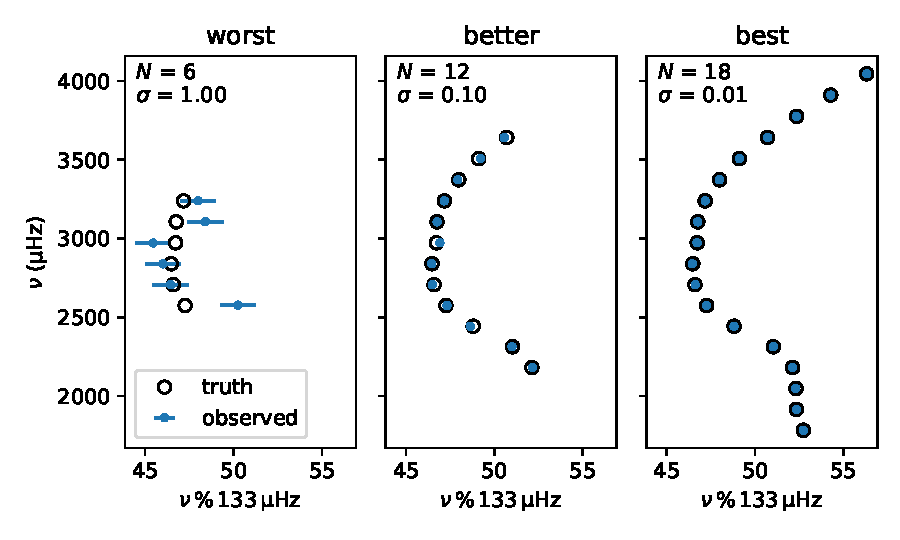
\includegraphics{figures/glitch-test-obs.pdf}
    \caption{Echelle plot of simulated true and `observed' radial mode frequency data from model star S for worst, better, and best case scenarios.}
    \label{fig:glitch-test-obs}
\end{figure}

\paragraph{Test Star} We created three sets of test data for worst, better, and best case scenarios using stellar model S (defined in Section \ref{sec:model-s}). Model S is similar to the Sun, with surface parameters of \(\teff = \SI{5682}{\kelvin}\), \(\log g = 4.426\) and \([\mathrm{Fe/H}] = 0.03\), and bulk parameters of \(M = \SI{1.00}{\solarmass}\), \(R = \SI{1.01}{\solarmass}\) and \(t_\star = \SI{4.07}{\giga\year}\). We calculated radial order modes (\(l=0\)) for the test star using the \textsc{GYRE} oscillation code \citep{Townsend.Teitler2013}. Then, we selected different numbers of modes (\(N\)) symmetrically about a reference frequency, \(\nu_\mathrm{ref} = \SI{2900}{\micro\hertz}\) (close to the expected frequency at maximum power of the star). To the frequencies, we added Gaussian noise scaled by \(\sigma_\obs = 1.0\), \(0.1\), and \SI{0.01}{\micro\hertz}, for the worst, better, and best cases respectively. The parameters and mode frequencies for each test case are shown in Table \ref{tab:glitch-obs}. We also plotted the modes on an echelle diagram in Figure \ref{fig:glitch-test-obs}. We can see the effect of the helium glitch in the echelle diagrams, where there is a periodic feature which is strongest at low frequencies. The glitch signature is visible in the better case and clearest in the best case scenario.

\paragraph{16 Cyg A} We used the asteroseismic benchmark star 16 Cyg A as an example real star to test both methods. We adopted values for 16 radial mode frequencies identified by \citet{Lund.SilvaAguirre.ea2017} using observations from \emph{Kepler} \citep[][KIC 12069424]{Borucki.Koch.ea2010}. The mode frequencies and their associated uncertainties are given in Table \ref{tab:glitch-obs}. The glitch has been previously studied for 16 Cyg A with its binary companion 16 Cyg B in \citet{Verma.Faria.ea2014}, making it a useful subject for comparison. Similarly to model S, this target is a solar analogue. However, it is slightly hotter, more evolved and more metal-rich, with \(\teff = \SI{5825(50)}{\kelvin}\), \(\log g = \SI{4.33(7)}{\dex}\) and \([\mathrm{Fe/H}] = \SI{0.10(3)}{\dex}\) \citep{Ramirez.Melendez.ea2009}. Its fundamental stellar parameters are \(M \approx \SI{1.1}{\solarmass}\), \(R \approx \SI{1.2}{\solarradius}\) and \(t_\star \approx \SI{7}{\giga\year}\) \citep{SilvaAguirre.Lund.ea2017}.

\section{Methods}\label{sec:glitch-methods}

In this section, we describe the two models for radial mode frequency, \(\nu_n = f(n, 0)\), and the fitting methods being compared in this work. The first is the \citetalias{Verma.Raodeo.ea2019} method, originally used in \citet{Verma.Faria.ea2014} to study the 16 Cyg binary star system. Secondly, we introduce our new `GP method'. Both methods use different statistical philosophy and formulation of the smoothly varying component, \(\tilde{f}(n)\). However, they each fit the same glitch component \(\delta\nu = \delta\nu_\helium + \delta\nu_\bcz\) as given in Equations \ref{eq:he-glitch} and \ref{eq:bcz-glitch}.

\subsection{The V19 Method}

The \citetalias{Verma.Raodeo.ea2019} method is a specific case of Equation \ref{eq:general-glitch}, where the smooth component is approximated by 4-th order polynomial,
%
\begin{equation}
    f_A(n) = \tilde{f}_A(n) + \delta\nu_\helium + \delta\nu_\bcz; \quad \tilde{f}_A(n) = \sum_{k=0}^{4} b_k n^k,
\end{equation}
%
\sloppy where \(b_k \equiv a_{0k} \nu_0\) from Equation \ref{eq:poly}. The model parameters are given by \(\vect{\theta}_A = (b_0, \dots, b_4, a_\helium, \beta_\helium, \tau_\helium, \phi_\helium, a_\bcz, \tau_\bcz, \phi_\bcz)\), where the glitch amplitude parameters are modified to include \(\nu_0\) such that \(a_i \equiv \alpha_i\nu_0\). The \(\nu_0\) parameter is not explicitly included in the \citetalias{Verma.Raodeo.ea2019} model, but we find it useful to keep the scaling in mind, and we use \(\nu_0\) in the GP model. 

The model parameters are optimised by minimising a \(\chi^2\) cost function with a regularisation term,
%
\begin{equation}
    \chi^2 = \sum_n \left[ \frac{\nu_n^\obs - f_{A}(n)}{\sigma_n^\obs} \right]^2 + \lambda^2 \sum_n \left[ \frac{\dd^3}{\dd n^3} \tilde{f}_A(n)\right]^2,
\end{equation}
%
where \(\nu_n^\obs\) and \(\sigma_n^\obs\) are the observed mode and its uncertainty at radial order \(n\), and \(\lambda\) is the regularisation parameter. The regularisation was used to avoid the polynomial over-fitting and absorbing the glitch terms.

We fitted the model using the \textsc{GlitchPy} code\footnote{\url{https://github.com/alexlyttle/GlitchPy}, adapted from \url{https://github.com/kuldeepv89/GlitchPy}.}. The fitting method is described in \citet{Verma.Raodeo.ea2019}, in which we adopted the same value of \(\lambda=7\) and bounds for the selection of initial parameters. We chose the initial parameters randomly within their bounds and optimised them using a BFGS minimisation of \(\chi^2\) \citep{Fletcher1987}, repeated 200 times until a global minimum was found. We further repeated this for 1000 realisations of the observed \(\nu_n\) with Gaussian noise scaled by \(\sigma_n^\obs\) to obtain a range of possible solutions.

\subsection{The GP Method}

In the second method, we used a Gaussian Process \citep[GP; see][for a recent review]{Aigrain.Foreman-Mackey2022} instead of a high-order polynomial to model the smoothly varying component of the mode frequencies. The GP represents a probability distribution in function-space, meaning that we can quantify the uncertainty associated with the functional form of $f$. We write our model for a set of modes \(\vect{n} = \{n_i\}_{i=1}^N\) as a random draw from a GP,
%
\begin{equation}
    f_{B}(\vect{n}) \sim \mathcal{GP}\left[ m(\vect{n}), k(\vect{n}, \vect{n}') \right],%\text{\footnotemark}
\end{equation}
%
% \footnotetext{In this section we use the convention that some random variable \(y\) drawn from a distribution \(q\) given parameters \(x\) may be written as \(y \sim q(x)\).}%
where \(m\) and \(k\) are the mean and kernel functions, and \(\vect{n}'\) is any other set of radial orders, \(\vect{n}' = \{n'_j\}_{j=1}^M\). The mean function describes where we expect \(\nu_n\) to be given some approximate physical reasoning. Therefore, we define our mean function for any \(n\)-th order mode as,
%
\begin{equation}
    m(n) = \tilde{f}_B(n) + \delta\nu_\helium + \delta\nu_\bcz; \quad \tilde{f}_B(n) = (n + \varepsilon) \nu_0, \label{eq:asy-glitch}
\end{equation}
%
where \(\tilde{f}_B(n)\) is the asymptotic approximation of the mode frequency (see Equation \ref{eq:asy}).

The kernel represents the expected covariance between the values of the function at different \(n\). We chose the squared exponential kernel function to be compatible with a smoothly-varying function of \(n\). Evaluating the kernel gives an \(N \times M\) matrix with an element \((i,j)\) given by,
%
\begin{equation}
    k(n_i, n'_j) = \alpha_k \nu_0 \, \ee^{- (n_i - n'_j)^2 / 2\lambda_k^2},
\end{equation}
%
where \(\alpha_k\) is a dimensionless amplitude scale factor and \(\lambda_k\) is the length scale (in units of radial order). Both kernel parameters control the flexibility of the GP. The amplitude parameter scales the covariance and \(\lambda_k\) describes the breadth of correlation between different modes. As \(\lambda_k \rightarrow 0\), the off-diagonal terms of the kernel approach zero producing uncorrelated noise with a variance of \(\alpha_k\nu_0\). We found values of \(\alpha_k = 0.5\) and \(\lambda_k = 5\) predicted smoothly varying functions compatible with our prior expectation.

The GP likelihood for some set of observations \(\vect{\nu}_\obs = \{\nu_{n_i}^\obs\}_{i=1}^N\) is a multivariate normal distribution centred on the mean function with covariance provided by the kernel function. We also added Gaussian noise terms to the diagonal of the covariance matrix,
%
\begin{equation}
    \vect{\nu}_\obs \sim \mathcal{N}\left( \vect{\mu}, \,  \vect{\Sigma} \right); \quad \vect{\Sigma} = \vect{K} + \mathrm{diag}(\sigma^2 + \vect{\sigma}_\obs^2), \label{eq:gp-like}
\end{equation}
%
where \(\vect{\mu} = m(\vect{n})\) and \(\vect{K} = k(\vect{n}, \vect{n})\). The scales of Gaussian noise in the model and observations are \(\sigma\) and \(\vect{\sigma}_\obs\) respectively. We included \(\sigma\) to account for uncorrelated noise in the model, for example from the difference between \(\delta\nu\) evaluated at \(\tilde{f}_B(n)\) and at the `true' mode frequencies.

To make noiseless predictions of mode frequencies \(\vect{\nu}_\star\) at new radial orders \(\vect{n}_\star\), we drew from the following multivariate normal distribution \citep{Rasmussen.Williams2006},
%
\begin{equation}
    \vect{\nu}_\star \mid \vect{\nu}_\obs \sim \mathcal{N} \left[ \vect{\mu}_\star + \vect{K}_\star^\mathsf{T} \, \vect{\Sigma}^{\,-1} \, (\vect{\nu}_\obs - \vect{\mu}), \, \vect{K}_{\star\star} - \vect{K}_\star^\mathsf{T} \, \vect{\Sigma}^{\,-1} \, \vect{K}_\star \right]
\end{equation}
%
where,
%
\begin{equation*}
    \vect{\mu}_\star = m(\vect{n}_\star), \quad \vect{K}_\star = k(\vect{n}, \vect{n}_\star), \quad \vect{K}_{\star\star} = k(\vect{n}_\star, \vect{n}_\star).
\end{equation*}
%
% This satisfies the consistency requirement that GP must specify any mode \(\nu_n \sim \mathcal{N}(\mu_n, K_{nn})\) where \(K_{nn}\) is the sub-matrix of the covariance of 

We used Bayes' theorem (see Equation \ref{eq:bayes}) to estimate the probability of our model parameters, \(\vect{\theta}_B = (\nu_0, \varepsilon, \alpha_\helium, \beta_\helium, \tau_\helium, \phi_\helium, a_\bcz, \tau_\bcz, \phi_\bcz, \sigma)\), given observations of mode frequencies. Hence, we write the posterior probability density as,
%
\begin{equation}
    p(\vect{\theta}_B \mid \vect{\nu}_\obs) = \frac{p(\vect{\nu}_\obs \mid \vect{\theta}_B)\,p(\vect{\theta}_B)}{p(\vect{\nu}_\obs)} \equiv \frac{\mathcal{L}(\vect{\theta}_B)\,p(\vect{\theta}_B)}{\mathcal{Z}},
\end{equation}
%
where \(\mathcal{L}(\vect{\theta}_B)\) is the likelihood of the data given the model, \(p(\vect{\theta}_B)\) is the prior probability density of the model parameters, and \(\mathcal{Z}\) is the `evidence' (or normalisation). The true posterior density function cannot be derived analytically, so we estimated it with the `nested sampling' algorithm \citep{Skilling2004}. By evaluating the prior volume at contours of constant likelihood, nested sampling estimates \(\mathcal{Z}\) to weight samples according to their posterior probability. This method requires functions for the log-likelihood and a transform which maps random samples in the unit hypercube to prior parameter space. 

\begin{table}
    \centering
    % \caption{The mean and variance for the prior normal distributions on each parameter where values are not explicitly given in the text.}
    \caption[The GP model parameters and their prior distributions.]{The GP model parameters and their prior distributions. Normal distributions are parametrised by the mean and variance (i.e. \(\mathcal{N}(\mu,\sigma^2)\)). Uniform distributions are parametrised by their lower and upper bounds.}
    \label{tab:glitch-prior}
    \begin{tabular}{lll}
\toprule
Parameter & \multicolumn{2}{c}{Prior} \\
\midrule
 & Test Star & 16 Cyg A \\
\midrule
$\nu_0/\si{\micro\hertz}$ & $\mathcal{N}(132.8,0.01)$ & $\mathcal{N}(103.28,0.0025)$ \\ 
$\varepsilon$ & $\mathcal{N}(1.4,0.0025)$ & $\mathcal{N}(1.45,0.0025)$ \\ 
$\ln(\alpha_\mathrm{cz}/\si{\micro\hertz\squared})$ & $\mathcal{N}(8.29,0.64)$ & $\mathcal{N}(8.04,0.64)$ \\ 
$\ln(\alpha_\mathrm{He}/\si{\mega\second})$ & $\mathcal{N}(-11.1,0.04)$ & $\mathcal{N}(-10.85,0.04)$ \\
$\ln(\beta_\mathrm{He}/\si{\mega\second\squared})$ & $\mathcal{N}(-15.07,0.16)$ & $\mathcal{N}(-14.56,0.16)$ \\
$\ln(\tau_\mathrm{cz}/\si{\mega\second})$ & $\mathcal{N}(-6.09,0.04)$ & $\mathcal{N}(-5.84,0.04)$ \\
$\ln(\tau_\mathrm{He}/\si{\mega\second})$ & $\mathcal{N}(-7.19,0.04)$ & $\mathcal{N}(-6.94,0.04)$ \\
$\ln(\sigma/\si{\micro\hertz})$ & $\mathcal{N}(- 4.605, 4)$ & $\mathcal{N}(- 4.605, 4)$ \\
$\phi_\helium, \phi_\bcz$ & $\mathcal{U}(0, 2\pi)$ & $\mathcal{U}(0, 2\pi)$ \\
\bottomrule
\end{tabular}

\end{table}

Following Equation \ref{eq:gp-like}, we defined the log-likelihood of the model as,
%
\begin{equation}
    \ln\mathcal{L}_B = - \frac12 \left[ {(\vect{\nu}_\obs - \vect{\mu})^\mathsf{T} \vect{\Sigma}^{\,-1} (\vect{\nu}_\obs - \vect{\mu})} + \ln(| \vect{\Sigma} |) + N\ln(2 \pi) \right],
\end{equation}
%
where \(\vect{\mu}\) and \(\vect{\Sigma}\) depend on \(\vect{\theta}_B\). The prior transform for \(\vect{\theta}_B\) is the inverse cumulative distribution function associated with the prior distribution \(p(\vect{\theta}_B)\). We treated the prior for each of \(\vect{\theta}_B\) independently. The total prior distribution is the product of distributions for each parameter, \(p(\vect{\theta}_B) = \prod_j p(\theta_{j})\). We give the prior distributions and their shape parameters in Table \ref{tab:glitch-prior}. In the following paragraphs, we justify our choice of prior distributions based on approximate scaling relations between the parameters. % We also summarise the prior distributions and their parameters in Table \todo{Table summary}

\paragraph{Smooth Component} Starting with the parameters for \(\tilde{f}_B(n)\), we chose to sample them from normal distributions,
%
\begin{gather}
    \nu_0 \sim \mathcal{N}(\overline{\nu}_0, s_{\nu_0}^2), \quad \varepsilon \sim \mathcal{N}(\overline{\varepsilon}, s_\varepsilon^2),%\\
    % \phi_\helium, \phi_\bcz \sim \mathcal{U}\left(0, 2\pi\right),
\end{gather}
%
centred on \(\overline{\nu}_0\) and \(\overline{\varepsilon}\) and scaled by \(s_{\nu_0}\) and \(s_\varepsilon\). For example, the location and scale parameters could come from global estimates of \(\langle\Delta\nu_n\rangle\) or a linear fit to the modes. We determined \(\overline{\nu}_0\) and \(\overline{\varepsilon}\) for the test stars from a linear fit to the true mode frequencies, and added representative uncertainties of 10 and 5 per cent respectively. For 16 Cyg A, we used measurements of \(\langle\Delta\nu_n\rangle\) and \(\nu_{\max}\) from \citet{Lund.SilvaAguirre.ea2017} to estimate \(\overline{\nu}_0\) and \(\overline{\varepsilon}\).

% Priors for the following parameters follow a log-normal distribution to ensure they are positive. We also exploit the property that the scale of a normal distribution in natural log-space is approximately the scale in real-space as a fraction of the distribution mean.

\paragraph{Acoustic Depths} We derived a prior on \(\tau_\helium\) and \(\tau_\bcz\) by observing how they scale with acoustic radius (\(\tau_0\)) in the grid of stellar models from \citet{Lyttle.Davies.ea2021} and in \citet{Verma.Rorsted.ea2022}. Typically, the fractional depth of He\,\textsc{ii} ionisation and the BCZ are \(\tau_\heII/\tau_0 \approx 0.2\) and \(\tau_\bcz/\tau_0 \approx 0.6\), for main sequence solar-like oscillators (see, e.g. Figure \ref{fig:gamma-sound-speed}). We formed the prior distributions from these relations, estimating the acoustic radius from \({\tau}_0 = (2\nu_0)^{-1}\). To account for possible variance with stellar properties, we added a spread of 20 per cent. We defined their priors in natural log-space to ensure they remained positive,
%
\begin{gather}
    \ln\tau_\helium \sim \mathcal{N}\left[ \ln(\overline{\tau}_\helium), \, s_{\ln\tau}^2 \right], \quad \ln\tau_\bcz \sim \mathcal{N}\left[\ln(3\,\overline{\tau}_\helium), \, s_{\ln\tau}^2 \right],\\
    \overline{\tau}_\helium = (10\,\overline{\nu}_0)^{-1}, \quad s_{\ln\tau}^2 = (1/5)^2 + (s_{\nu_0}/\overline{\nu}_0)^2.
\end{gather}

\paragraph{Helium Glitch Amplitude} Deriving a prior on the glitch amplitude parameters was less trivial. By observing \(\gamma\) profiles in the grid of stellar models, we assumed that the width of the helium ionisation region was about 8 per cent of the acoustic depth of the region, \(\Delta_\heII/\tau_\heII \approx 0.08\). Thus, we centred the prior on \(\overline{\beta}_\helium\) obtained from this assumption and used the relation \(\beta_\helium = 8\pi^2\Delta_\heII^2\) from comparison to Equation \ref{eq:he-osc}. We then propagated the variance from the prior on \(\tau_\helium\),
%
\begin{equation}
    \ln\beta_\helium \sim \mathcal{N}\left[ \ln(\overline{\beta}_\helium), \, 4 s_{\ln\tau}^2 \right], \quad \overline{\beta}_\helium = \frac{32}{625} \, \pi^2 \overline{\tau}_\helium^2.
\end{equation}
%
Then, we centred the prior for \(\alpha_\helium\) to satisfy a depth of 0.1 in \(\delta\gamma/\gamma\) caused by helium ionisation using Equation \ref{eq:he-gamma},
%
\begin{gather*}
    \ln\alpha_\helium \sim \mathcal{N}\left[ 1/2 \, \ln({\overline{\beta}_\helium}/{400\pi}), \, s_{\ln\tau}^2 \right].
\end{gather*}
%
We verified that the priors on \(\alpha_\helium\) and \(\beta_\helium\) were compatible with our prior belief by checking that the amplitude at \(\nu_\mathrm{ref}\) peaked from \SIrange{0}{1}{\micro\hertz}, decaying thereafter.

\paragraph{BCZ Glitch Amplitude} We constructed the prior on \(\alpha_\bcz\) such that the BCZ glitch amplitude was approximately \SI{0.1}{\micro\hertz} at \(\nu_\mathrm{ref}\) (an order of magnitude smaller than the helium glitch). This occurred when \(\alpha_\bcz/\nu_0 \approx \SI{30}{\micro\hertz}\). We also scaled the distribution by an additional 80 per cent,
%
\begin{equation*}
    \ln\alpha_\bcz \sim \mathcal{N}\left[ \ln(30\,\overline{\nu}_0), \, (4/5)^2 + (s_{\nu_0}/\overline{\nu}_0)^2\right].
\end{equation*}
%

% \begin{table}
%     \centering
%     % \caption{The mean and variance for the prior normal distributions on each parameter where values are not explicitly given in the text.}
%     \caption[The GP model parameters and their prior distributions.]{The GP model parameters and their prior distributions. Normal distributions are parametrised by the mean and variance (i.e. \(\mathcal{N}(\mu,\sigma^2)\)). Uniform distributions are parametrised by their lower and upper bounds.}
%     \label{tab:glitch-prior}
%     \begin{tabular}{lll}
\toprule
Parameter & \multicolumn{2}{c}{Prior} \\
\midrule
 & Test Star & 16 Cyg A \\
\midrule
$\nu_0/\si{\micro\hertz}$ & $\mathcal{N}(132.8,0.01)$ & $\mathcal{N}(103.28,0.0025)$ \\ 
$\varepsilon$ & $\mathcal{N}(1.4,0.0025)$ & $\mathcal{N}(1.45,0.0025)$ \\ 
$\ln(\alpha_\mathrm{cz}/\si{\micro\hertz\squared})$ & $\mathcal{N}(8.29,0.64)$ & $\mathcal{N}(8.04,0.64)$ \\ 
$\ln(\alpha_\mathrm{He}/\si{\mega\second})$ & $\mathcal{N}(-11.1,0.04)$ & $\mathcal{N}(-10.85,0.04)$ \\
$\ln(\beta_\mathrm{He}/\si{\mega\second\squared})$ & $\mathcal{N}(-15.07,0.16)$ & $\mathcal{N}(-14.56,0.16)$ \\
$\ln(\tau_\mathrm{cz}/\si{\mega\second})$ & $\mathcal{N}(-6.09,0.04)$ & $\mathcal{N}(-5.84,0.04)$ \\
$\ln(\tau_\mathrm{He}/\si{\mega\second})$ & $\mathcal{N}(-7.19,0.04)$ & $\mathcal{N}(-6.94,0.04)$ \\
$\ln(\sigma/\si{\micro\hertz})$ & $\mathcal{N}(- 4.605, 4)$ & $\mathcal{N}(- 4.605, 4)$ \\
$\phi_\helium, \phi_\bcz$ & $\mathcal{U}(0, 2\pi)$ & $\mathcal{U}(0, 2\pi)$ \\
\bottomrule
\end{tabular}

% \end{table}

% The mean and variance for the aforementioned prior distributions are summarised in Table \ref{tab:glitch-prior} for the test star and 16 Cyg A. 
Prior distributions for the remaining parameters were the same for both stars. For example, the prior on the phase parameters \(\phi_\helium\) and \(\phi_\bcz\) was uniformly distributed from 0 to \(2\pi\). We also used a weakly informative prior on the model uncertainty, \(\ln\sigma \sim \mathcal{N}( - \ln 100, 4)\), centred on \SI{0.01}{\micro\hertz}.

We sampled the posterior distribution using the \textsc{Python} nested sampling package \texttt{dynesty} \citep{Speagle2020,Koposov.Speagle.ea2023}. We applied the multi-ellipsoid bounding method \citep{Feroz.Hobson.ea2009} with 500 live points and the random walk sampling method \citep{Skilling2006} with a minimum of 50 steps before proposing a new live point. In addition, we enabled periodic boundary conditions for \(\phi_\helium\) and \(\phi_\bcz\) with the prior transform projecting to periodic space using \(\phi = \phi'\,\mathrm{mod}\,2\pi\), where \(\phi'\) is unconstrained. Otherwise, the nested sampler ran with its default parameters. We used the \textsc{Python} package \texttt{jax} \citep{Bradbury.Frostig.ea2018} to make use of accelerated linear algebra (XLA) and just-in-time (JIT) compilation, and \texttt{tinygp} \citep{Foreman-Mackey.Yadav.ea2022} to build the GP. For analysis and comparison with the \citetalias{Verma.Raodeo.ea2019} method, we drew 1000 points randomly from the posterior samples according to their estimated weights.

% Rearranged into dimensionless quantities, \(f = \nu/\nu_0\), \(t = \tau/\tau_0\), \(a_\helium = \nu_0\alpha_\helium\), \(b_\helium = \nu_0 \beta_\helium\), and \(a_\bcz = \alpha_\bcz/\nu_0^2\),
% %
% \begin{align}
%     f_n &\simeq f_\asy + \delta f_\helium + \delta f_\bcz\\
%     \delta f_\helium &= a_\helium f \, \ee^{-b_\helium f^2} \sin(2 \pi \, t_\helium f + \phi_\helium),\\
%     \delta f_\bcz &= a_\bcz f^{-2} \, \sin(2\pi\,t_\bcz f + \phi_\bcz)
% \end{align}
% %

\section{Results}\label{sec:glitch-results}

% In this section, we compare the results from both methods on the test star and 16 Cyg A.

% \todo{3 model stars with different helium abundance}.

\subsection{Test Star}

\begin{figure}[!tb]
    \centering
    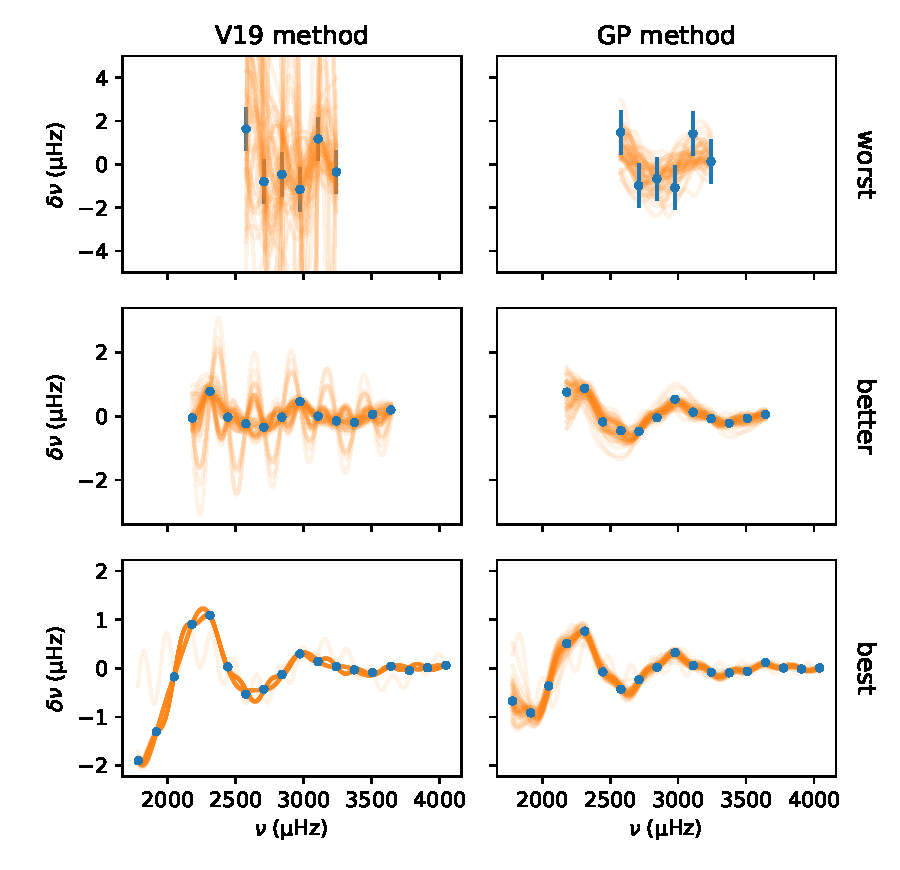
\includegraphics{figures/glitch-test-signal.pdf}
    \caption[50 random draws from the V19 and GP results showing the total glitch signal as a function of frequency.]{50 random draws from the V19 and GP methods showing the total glitch signal, \(\delta\nu = \delta_\helium(\nu) + \delta_\bcz(\nu)\), as a function of frequency, \(\nu\). The data points plot in blue are the median smooth component model at \(\vect{n}\), subtracted from the observed modes (\(\vect{\nu}_\obs\)) with their observed uncertainty (\(\sigma_\obs\)).}
    \label{fig:glitch-test-signal}
\end{figure}

In Figure \ref{fig:glitch-test-signal}, we plot the predicted total glitch component (\(\delta\nu\)) using 50 draws from the posterior distribution for both methods. We subtracted the median smooth component (\(\tilde{f}(n)\)) from the observed \(\nu_n\) over-plot. For each scenario, both methods predicted similar glitch components. However, the \citetalias{Verma.Raodeo.ea2019} method showed more extreme multimodality in all cases. For example, the better case showed a high-amplitude (\(\sim \SI{2}{\micro\hertz}\)) BCZ glitch solution which is not present with the GP method. Such a large BCZ signature would be unlikely. Additionally, the two methods differed by \(\sim \SI{1}{\micro\hertz}\) at low frequency in the best case. Despite this, the \citetalias{Verma.Raodeo.ea2019} method appeared to be more confident in its glitch solutions compared to the GP method.

\begin{figure}[!tb]
    \centering
    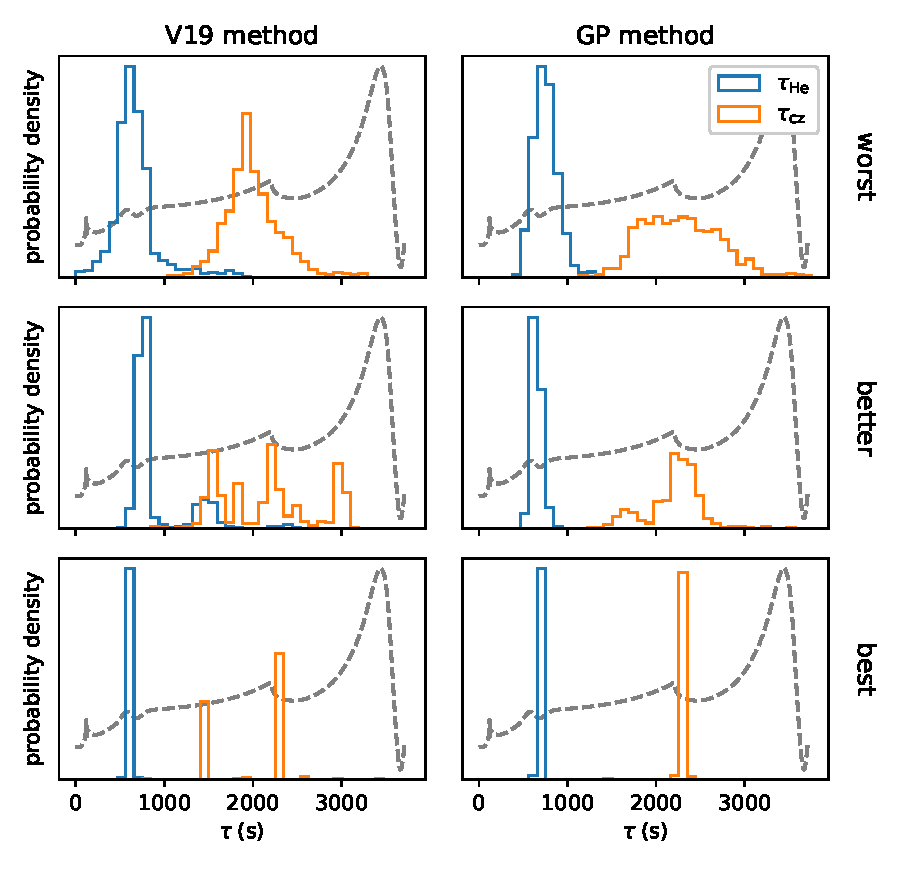
\includegraphics{figures/glitch-test-tau.pdf}
    \caption[Samples from the V19 and GP methods for the acoustic depths of the helium glitch (\(\tau_\helium\)) and base of the convective zone (\(\tau_\bcz\))]{Samples from the V19 and GP methods for the acoustic depths of the helium glitch (\(\tau_\helium\)) and base of the convective zone (\(\tau_\bcz\)). The sound-speed gradient from Figure \ref{fig:sound-speed-gradient} is over-plot with a grey dashed line.}
    \label{fig:glitch-test-tau}
\end{figure}

In Figure \ref{fig:glitch-test-tau}, we plotted posterior distributions for the glitch acoustic depths, \(\tau_\helium\) and \(\tau_\bcz\), and compared them to the sound speed gradient of the test star from Figure \ref{fig:sound-speed-gradient}. We expect the acoustic depths to approximately line up with the sharp structural changes. For the worst case, both methods gave broad distributions for the acoustic depths, compatible with their respective initial guesses and priors. The \citetalias{Verma.Raodeo.ea2019} method initial guesses appeared to underestimate \(\tau_\bcz\), whereas the GP method prior was broad enough to encompass a wide range of possible \(\tau_\bcz\). In the better and best cases, we found that the \citetalias{Verma.Raodeo.ea2019} solutions were multimodal. For example, the better case found solutions for \(\tau_\helium\) far deeper into the star than we would expect, at around \SI{1500}{\second} and \SI{2500}{\second}.

% As predicted by \citet{Houdek.Gough2007} and shown in \citet{Verma.Faria.ea2014}... This is because \(\delta\nu_\helium\) does not include the smaller glitch component due to the first ionisation of helium, located at a smaller \(\tau\).
The values for \(\tau_\helium\) obtained were under-predicted compared to the location of the trough due to the second ionisation of helium. We can see this for the best star fit with the \citetalias{Verma.Raodeo.ea2019} method which finds \(\tau_\helium = \SI{619(15)}{\second}\). The depression in \(\gamma\) due to He\,\textsc{ii} ionisation in the respective stellar model is located at \SI{733}{\second}. On the other hand, the GP method was closer with \(\tau_\helium = \SI{696(19)}{\second}\).

\begin{figure}[tb]
    \centering
    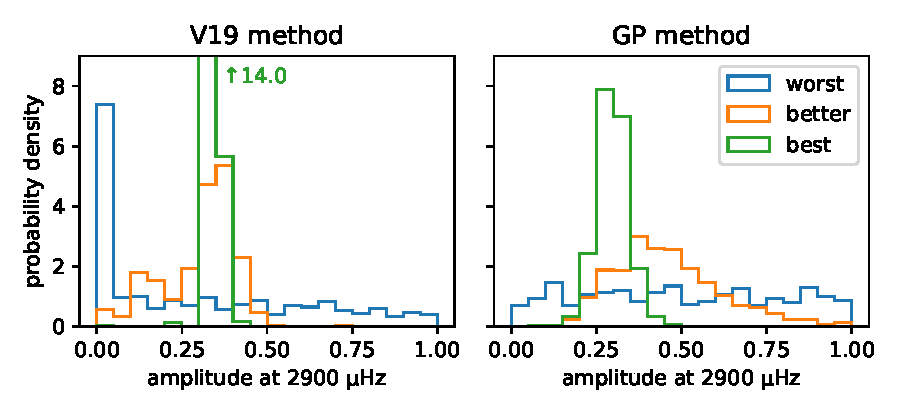
\includegraphics{figures/glitch-test-amplitude.pdf}
    \caption[Samples of the helium glitch amplitude at a reference frequency of \SI{3000}{\micro\hertz} fit with the V19 and GP methods for the worst, better, and best case test data.]{Samples of the helium glitch amplitude at a reference frequency of \SI{3000}{\micro\hertz} fit with the V19 and GP methods for the worst, better, and best case test data. The tallest bar in the V19 method panel is cropped with its value displayed in green text.}
    \label{fig:glitch-test-amplitude}
\end{figure}

We compared helium glitch amplitudes at \(\nu_\mathrm{ref}\) from both methods in Figure \ref{fig:glitch-test-amplitude}. The \citetalias{Verma.Raodeo.ea2019} method preferred low-amplitude solutions for the worst and better cases compared to the GP method. On the other hand, the GP method reflected our prior in the worst case, with the width of the distribution shrinking as the data improved. The GP method did show some bi-modality in the better case, with higher solutions at \(A_\helium^\mathrm{ref} \approx 0.7\) which were not found by the \citetalias{Verma.Raodeo.ea2019} method. In the best case, the \citetalias{Verma.Raodeo.ea2019} method obtained \(A_\helium^\mathrm{ref} = 0.347_{-0.005}^{+0.006}\), whereas the GP method found \(A_\helium^\mathrm{ref} = 0.296_{-0.036}^{+0.042}\).

% Why not use delta gamma / gamma as the probe of helium abundance? That is proportional to alpha / sqrt(beta). Then, an update to this method can use this and beta as a parameter and then work out alpha from that, since beta should scale with tau and the depth is a signature of helium abundance. Be careful as number of modes correlates with delta nu value of fit.

\subsection{16 Cyg A}

We compared the results from both methods applied to the 16 Cyg A data in Figure \ref{fig:glitch-16cyga}. We found that the \citetalias{Verma.Raodeo.ea2019} method predicted extreme solutions for the glitch where the GP method did not. There was also a difference of about \SI{1}{\micro\hertz} at the low frequency end such that the \citetalias{Verma.Raodeo.ea2019} predicted a larger glitch amplitude. Otherwise, the two methods gave similar solutions for the glitch function.

Both methods found similar values for \(\tau_\helium\) but relatively different distributions for \(\tau_\bcz\). Regarding the helium glitch, the \citetalias{Verma.Raodeo.ea2019} method found \(\tau_\helium = 917_{-53}^{+50} \, \mathrm{s}\), and our GP method obtained \(\tau_\helium = 931_{-88}^{+59} \, \mathrm{s}\), within 1-\(\sigma\) of each other. Similarly to the test star, the GP method found a slightly larger value of \(\tau_\helium\) than the \citetalias{Verma.Raodeo.ea2019} method. \citet{Verma.Faria.ea2014} fit the glitch using \(l=0,1,2\) modes and found an acoustic depth of \SI{930(14)}{\second}, within 1-\(\sigma\) of both methods in this work.

We calculated the helium glitch amplitude at a reference frequency of \SI{2188.5}{\micro\hertz}, equivalent to \(\nu_{\max}\) obtained by \citet{Lund.SilvaAguirre.ea2017}. Samples from both posteriors are shown in the bottom panel of Figure \ref{fig:glitch-16cyga}. We found \(A_\helium^\mathrm{ref} = 0.260_{-0.065}^{+0.050}\,\si{\micro\hertz}\) for the \citetalias{Verma.Raodeo.ea2019} method, and \(A_\helium^\mathrm{ref} = 0.333_{-0.073}^{+0.081}\,\si{\micro\hertz}\) for the GP method. Both values were about 1-\(\sigma\) apart. Additionally, both methods found \(A_\bcz^\mathrm{ref} \sim 0.1\,\si{\micro\hertz}\), with the GP method favouring a smaller value. The \citetalias{Verma.Raodeo.ea2019} method found some solutions where \(A_\bcz^\mathrm{ref}\) was larger than \(A_\helium^\mathrm{ref}\), something we would not expect because the modes are less sensitive to structural changes deeper in the star.

\begin{figure}[!tb]
    \centering
    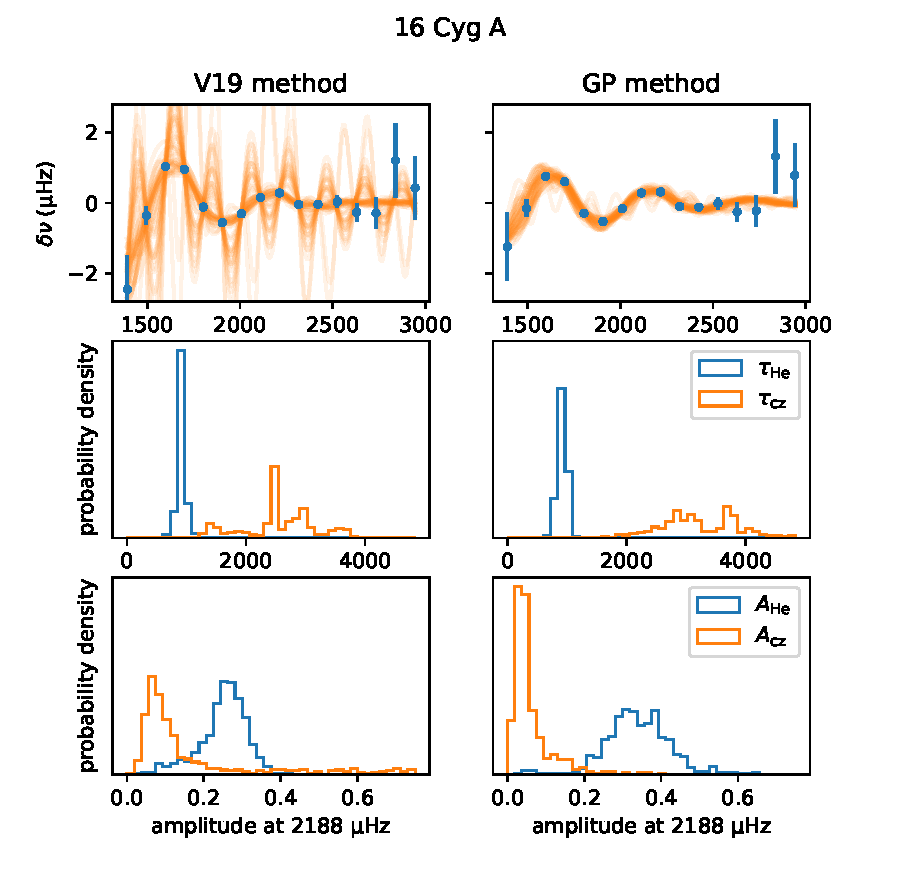
\includegraphics{figures/glitch-16cyga.pdf}
    \caption[Results for the glitch fit to 16 Cyg A using the V19 method and GP method.]{Results for the glitch fit to 16 Cyg A using the \citetalias{Verma.Raodeo.ea2019} method (\emph{left}) and GP method (\emph{right}). The top panel shows 50 draws from the posterior prediction of \(\delta\nu = \delta\nu_\helium + \delta\nu_\bcz\) with the observed \(\nu_n\) minus the median smooth background component of the model. The middle and bottom panels shows the posterior sample probability density for the acoustic depths and reference amplitudes of the glitches respectively.}
    \label{fig:glitch-16cyga}
\end{figure}

\section{Discussion}\label{sec:glitch-disc}

% Discuss major differences

\begin{figure}[tb]
    \centering
    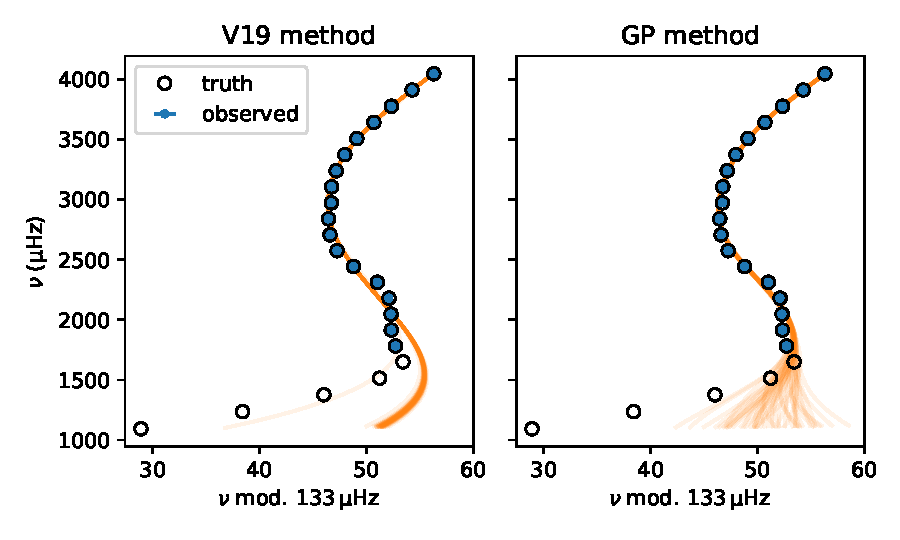
\includegraphics{figures/glitch-test-smooth.pdf}
    \caption[Echelle-like diagrams showing mode frequencies plot against their frequency modulo \SI{133}{\micro\hertz} for the best case scenario.]{Echelle-like diagrams showing mode frequencies plot against their frequency modulo \SI{133}{\micro\hertz} for the best case scenario. The orange lines show 50 draws from the model posterior predictions with the glitch component removed (\(f(n) - \delta\nu\)) for both methods. The predictions are made from a lower radial order \(n=8\) than the observed modes. The true values from model S are shown for each mode. Some radial orders (\(n\)) are shown next to the modes for context.}
    \label{fig:best-smooth}
\end{figure}

Throughout this work, we found a smaller \(\delta\nu\) amplitude at low frequency with the GP method than with the \citetalias{Verma.Raodeo.ea2019} method. This was particularly visible in the best case and in 16 Cyg A. We expected this was a result of the different smooth background models. In Figure \ref{fig:best-smooth} we plotted the smooth component of each model extended to lower order, unobserved modes. We found the GP background component had a turning point at \(\nu \approx \SI{1900}{\micro\hertz}\), higher than the \citetalias{Verma.Raodeo.ea2019} method at \(\nu \approx \SI{1500}{\micro\hertz}\). The smooth component of the \citetalias{Verma.Raodeo.ea2019} method was confidently incorrect outside the observed frequencies. Conversely, the GP method predicted closer to the truth with increasing uncertainty further from the observations. It appeared that the GP provided a more accurate representation of the underlying function than the polynomial.

\begin{figure}[!tb]
    \centering
    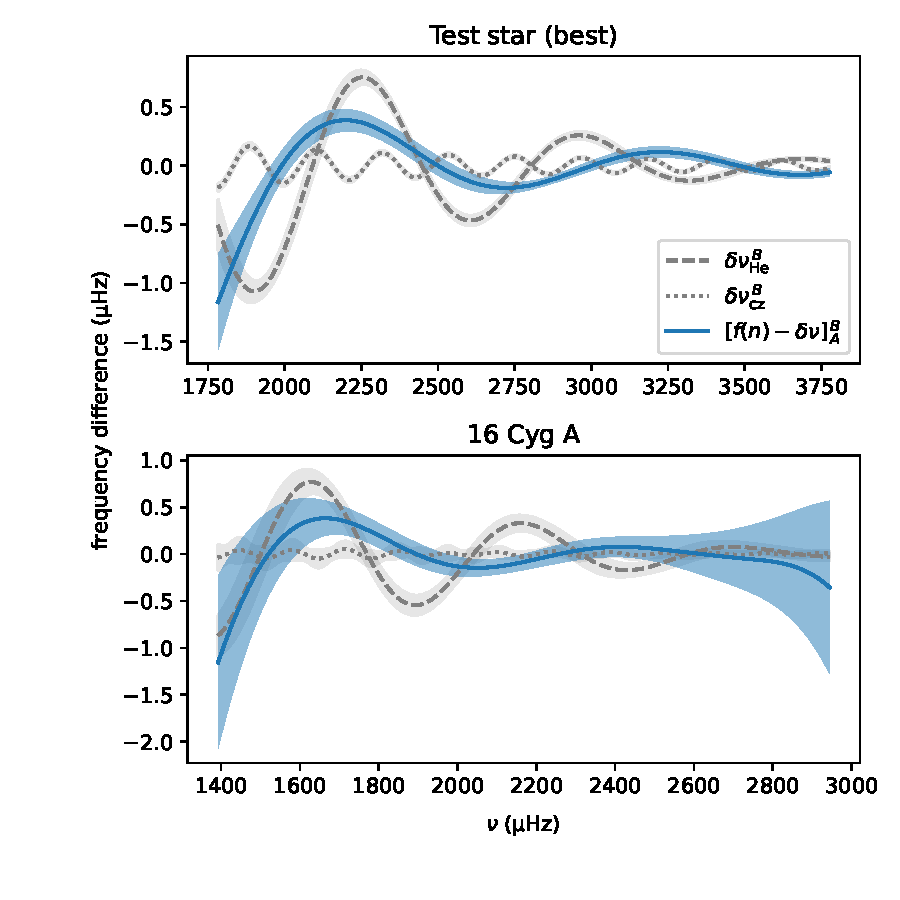
\includegraphics[trim={0.4in 0.2in 0 0},clip]{figures/glitch-res.pdf}
    \caption[The difference between the model without the glitch components predicted by theV19 method and the GP method.]{The difference between the model without the glitch components (\(f(n) - \delta\nu\)) predicted by the \citetalias{Verma.Raodeo.ea2019} method (A) and the GP method (B). The glitch components from the GP method are plot in grey for context. The 68 per cent confidence region is shaded for each line.}
    \label{fig:smooth-res}
\end{figure}

In the test star's best case and 16 Cyg A, the GP method found a higher \(\tau_\helium\) than the \citetalias{Verma.Raodeo.ea2019} method. This could be because the GP was better able to distinguish between the He\,\textsc{ii} glitch and the smaller He\,\textsc{i} glitch. To explore this, we plotted the difference between each model's predictions for the smooth component in Figure \ref{fig:smooth-res}. We saw a clear periodic signal in the differences. The period of this signal in the test star corresponded to an acoustic depth of \(\sim \SI{500}{\second}\), matching the location of He\,\textsc{i} ionisation in model S. The periodic signal was less pronounced for 16 Cyg A, but corresponded to a plausible He\,\textsc{i} acoustic depth of \(\sim \SI{700}{\second}\). We expected that the polynomial was not flexible enough to pick up the He\,\textsc{i} ionisation signature, hence lowering its mean value for \(\tau_\helium\).

% Discuss the prior

The \citetalias{Verma.Raodeo.ea2019} method found several extreme solutions for \(\delta\nu\) whereas GP method did not. We expected this because the GP method used a prior over the model parameters. We tested relaxing the prior on \(\vect{\theta}_B\) and found similar multimodal posteriors to the \citetalias{Verma.Raodeo.ea2019} method. This showed that the prior helped eliminate unrealistic solutions. However, care should be taken over the choice of prior on \(\vect{\theta}_B\) to realistically reflect our expectation. If some of our prior assumptions are incorrect, they may bias the results. For example, the outer convective region gets shallower as stars get hotter (approaching \(\teff \approx \SI{7000}{\kelvin}\)) making the assumption that \(\tau_\bcz/\tau_0 \approx 0.6\) an overestimate in these cases. We accommodate for this with a wide prior on \(\tau_\bcz\), but our prior could be more informed. There is a notable temperature dependence to \(\tau_\bcz/\tau_0\) observed in the grid of stellar models which could be exploited in the future when constructing the prior.

Additionally, the joint posteriors for \(\alpha_\helium\) and \(\beta_\helium\) were correlated in both methods. This was expected, because larger values of \(\beta_\helium\) can be compensated for with a larger amplitude factor (\(\alpha_\helium\)). In the GP method, we did not include this expected correlation in our prior. Hence, we found that having broader priors on \(\alpha_\helium\) and \(\beta_\helium\) lead to the prior predicting unrealistic glitches. We could account for this by using a multivariate prior for the amplitude parameters. Despite this, our approach still improves on the \citetalias{Verma.Raodeo.ea2019} method by using a prior in the first place.

A potential limitation of the GP method is that we calculate the glitch at \(\tilde{f}_B(n)\) from the linear asymptotic equation (Equation \ref{eq:asy}). In regions where the gradient of \(\delta\nu\) is high, the difference between \(\tilde{f}_B(n)\) and the true frequency can be up to \(\sim \SI{0.1}{\micro\hertz}\). Our choice of kernel function cannot absorb this difference because is varies on a short length-scale. Instead, we accounted for this uncertainty by adding Gaussian noise to the model parametrised by \(\sigma\). However, for the best test star, we found \(\sigma \approx 0.05\), which was larger than the observational uncertainty, \(\sigma_\obs = 0.01\). This could limit our method's inference ability for the best asteroseismic targets. One solution is to replace \(\tilde{f}_B(n)\) with a quadratic \citep[e.g.][]{Nielsen.Davies.ea2021} which better approximates \(\nu_n\). However, the GP kernel would need to be adjusted to account for this.

% Using the glitch parameters as a helium diagnostic could involve measuring the amplitude of the helium glitch at a reference frequency such as \(\nu_{\max}\). We should expect solutions for this reference amplitude (\(A_\mathrm{ref}\)) to converge on a value as the data quality increases from worst to best. It is also important that the uncertainty of the reference amplitude is accurate if using it to constrain helium abundance in a population of stars. If using V19 method on a population of stars, this could bias inference towards lower values of helium abundance.

\section{Conclusion}

We introduced a new method for modelling acoustic glitches in solar-like oscillators using a Gaussian Process. Testing the method on a model star, we found that it more accurately characterised the underlying, smoothly-varying functional form of the radial modes than the 
\citetalias{Verma.Raodeo.ea2019} method. Furthermore, our method appeared able to absorb the glitch component from He\,\textsc{i} ionisation, for which the polynomial was not flexible enough. However, this questions whether the He\,\textsc{i} ionisation glitch should be explicitly included in the model.

Additionally, the GP method provided more believable uncertainties on the glitch parameters, whereas the \citetalias{Verma.Raodeo.ea2019} method was over-confident with the best data and under-confident with the worst. Robust uncertainties are important when using the results to make further inference about helium enrichment. In this case, the GP marginalised over correlated noise in the model, not possible with the \citetalias{Verma.Raodeo.ea2019} method.

Future development of the method could involve building a prior for the glitch parameters. For example, we could start with fitting the model to simulated stars and using the results to build an empirical prior. Then, we could run the model on a larger asteroseismic sample of main sequence stars \citep[e.g.][]{Lund.SilvaAguirre.ea2017,Davies.SilvaAguirre.ea2016} and compare our results to those from \citet{Verma.Raodeo.ea2019}. Additionally, we could add parameters from the GP model to the hierarchical model introduced in \citet{Lyttle.Davies.ea2021}. Ultimately, our goal is to scale this method in anticipation of the \(\sim 10^4\) solar-like oscillators expected to be observed by \emph{PLATO} \citep{Rauer.Catala.ea2014}.

  % chapters/conclusion.tex
%
% Copyright 2022 Alexander Lyttle.
%
% This work may be distributed and/or modified under the conditions of the
% LaTeX Project Public License (LPPL) version 1.3 or later.
%
% The latest version of this license is in
% https://www.latex-project.org/lppl.txt and version 1.3 or later is part of
% all distributions of LaTeX version 2005/12/01 or later.
%
%
\chapter{Conclusion}

We demonstrated that a hierarchical Bayesian model (HBM) can improve the inference of inferred stellar parameters. Introducing the concept of an HBM in Chapter \ref{chap:hbm}, we showed how we can include population distributions in a prior to inform individual parameters within the population. We then applied an HBM to model a well-studied sample of oscillating dwarf and subgiant stars in Chapter \ref{chap:hmd}. While accounting for uncertainty in helium abundance and other physics, we were still able to achieve statistical uncertainties of 1.2 per cent in radius, 2.5 per cent in mass and 12 per cent in age. This provides a framework for modelling large populations of stars at the same time.

In our HBM, we assumed a linear helium enrichment law as the mean of a population distribution in initial stellar helium abundance. We marginalised over the uncertainty in the parameters of this law, improving upon other work which just assume a fixed value of the law \citep[e.g.][]{Serenelli.Johnson.ea2017}. We found the slope of this law (\(\Delta Y/\Delta Z\)) to be \(\approx 1\) with and \(\approx 1.6\) without including the Sun-as-a-star in our population. Although these were within 2-\(\sigma\) of each other, it was concerning that the Sun had such an extreme effect. We found signs of \(\teff\) scale offset which could be to blame for this, something we expect APOGEE spectroscopy \needcite. Therefore, future work should parametrise more sources of systematic uncertainty, such as a temperature scale offset.

\section{Improving the Hierarchical Model}

In Chapter \ref{chap:glitch}, we recalled that mode frequencies carry information about acoustic glitches inside the star. However, the form of these mode frequencies as a function of \(n\) is not exactly known. We showed that a Gaussian Process (GP) could be used to marginalise over the uncertainty in this functional form and improve detection of the helium glitch signature.  Our method showed promise compared to those which have come before \citep[e.g.][]{Verma.Raodeo.ea2019}, motivating a more quantatitive comparison in the future. We hope to build a more informed prior on the model parameters and publish this method soon with more examples.

The helium glitch parameters for a given star correlate with its near-surface helium abundance \citep{Houdek.Gough2007}. Therefore, a natural next step would be to include helium glitch parameters in our HBM. Our GP glitch model can be applied to both observed and modelled mode frequencies, providing extra parameters to include in our stellar model emulator (see Section \ref{sec:conc-nn}). Including these should improve inference of helium abundance for stars with individual modes identified \citep[e.g.][]{Davies.SilvaAguirre.ea2016,Lund.SilvaAguirre.ea2017}. Since our HBM models the population distribution of helium, even a small number of stars with good helium constraint will in-turn improve helium estimates for the rest of the population.

% We can also extend the hierarchical aspect of the model. There are other parameters which we expect to correlate in a population of stars. Binary star systems are likely to share common ages and chemical abundances. Some examples are 16 Cyg A and B with an age of \(\sim\SI{7}{\giga\year}\) \citep{Davies.Chaplin.ea2015,Metcalfe.Chaplin.ea2012}, and \(\alpha\) Cen A and B \citep{Kjeldsen.Bedding.ea2005,Bouchy.Carrier2002} with ages \(\sim\SI{6}{\giga\year}\) \citep{Bazot.Bourguignon.ea2012}. Since the masses of these systems are constrained independency of the models, they act as additional points of calibration within the model.

In Chapter \ref{chap:hmd}, we did not consider the effect of uncertain atmospheric physics which effects the mode frequencies. Surface correction methods exist, but ideally we would include this as an extra parameter. While these represented the lowest systematic uncertainty from the study by \citet{Nsamba.Campante.ea2018} compared with diffusion and solar metallicity mixture.

% Once we extend the model to red giants, we can also consider including population distributions on stellar clusters. For example, \emph{Kepler} observed open clusters NGC... which all include solar-like oscillators \needcite. We can 

\section{Emulating Stellar Models}\label{sec:conc-nn}

To emulate the stellar models, we found that a neural network could predict stellar observables with typical errors of up to \(\sim 0.1\) per cent (see Appendix \ref{apx:hmd}). This provided a simple, continuous and differentiable model mapping stellar parameters to observables. We found a notable advantage to using a neural network was its scalability. The linear algebra involved allows for fast predictions for a large numbers of stars in parallel. Furthermore, the neural network can be scaled up to higher input and output dimensions with little performance impact. For example, we recently trained a neural network to emulate the regularly spaced mode frequencies of \(\delta\) Scuti-type oscillators \citep{Scutt.Murphy.ea2023}. This demonstrated the method's applicability to other kinds of oscillators.

We also expect the neural network emulation method to scale to red giant solar-like oscillators. We trained the emulator on a grid of stellar models from the zero-age main sequence to the base of the red giant branch for masses from \SIrange{0.8}{1.2}{\solarmass}. On the main sequence, the upper mass limit was motivated by the diminishing outer convective envelope (responsible for driving solar-like oscillators) in these stars. However, extending the emulator to model red giant solar-like oscillators would require expanding the grid up to \(\sim\SI{2.0}{\solarmass}\). Extending the grid by mass alone, we would need to compute thrice as many evolutionary tracks and evolve existing models further. However, stars with \(M \gtrsim \SI{1.2}{\solarmass}\) have a convective core on the main sequence which introduces an additional model uncertainty from mixing at its boundary. Parametrising this would further multiply the number of input tracks. To handle more dimensions, we should research ways of selectively computing stellar models or augmenting the grid where the neural network error is large.

% Currently, we compute a grid of models where inputs are spaced regularly. However, the neural network may perform better in some regions and worse in others. We could create an algorithm which computes more stellar evolutionary tracks in regions of parameter space where the neural network performs poorly. This way we could start with a sparse grid of training data, then generate more tracks where the neural network error is high and retrain.

\section{Current and Future Data}

Recently, \citet{Hatt.Nielsen.ea2023} identified a sample of \(\sim 4000\) solar-like oscillators in 120- and 20-second cadence \emph{TESS} data. Of these, around 50 \todo{check} are dwarf and subgiant stars which we could include in a future iteration of the HBM. With larger sample sizes, we can further increase the precision of pooled parameters and better characterise their spread in the population distribution. However, we expect the sample size to increase by a few magnitudes by the end of the decade

% This has been exceptionally useful with galactic archaology with the \(\sim 150,000\) oscillating red giants detected by \citet{Hon.Huber.ea2021}. 

Towards the end of the 2020s, we expect the \emph{PLATO} mission to observe tens of thousands of dwarf and subgiant solar-like oscillators \citep{Rauer.Catala.ea2014}. \emph{PLATO} aims to discover hundreds more exoplanets orbiting solar-type stars across a wider proportion of the sky when compared to \emph{Kepler}. They expect to observe up to 20,000 bright (V < 11) oscillating F-K dwarf stars over two year periods \citep{Goupil2017}. Using our HBM method on a sample this size could see a reduction in uncertainty on helium abundance from 0.01 to 0.0005. While this is the maximum expected uncertainty reduction discussed in Chapter \ref{chap:hbm}, it shows that we can start to consider more complex population distributions in helium.

This also allows us to test more complex population-level distributions.  However, this approach may benefit more from extending the HMB to include red giants, for which \emph{Kepler} and \emph{TESS} have yielded \(\sim 100,000\) \citep{Hon.Huber.ea2021,Yu.Huber.ea2018}. For example, since \emph{TESS} is an all-sky survey, we could test including kinematics and galactic positions in the enrichment law. Comparable samples of main sequence stars will not arrive until the end of this decade.

% The number of dwarf and subgiant solar-like oscillators expected from \emph{PLATO} will be comparable to the number of red giant oscillators already found with \emph{Kepler} and \emph{TESS} \needcite. In the meantime we could test extending our method to red giant stars to make use of the abundance of data. This comes with additional challenges. Oscillating red giants include masses \(\gtrsim \SI{1.2}{\solarmass}\) which would have had a convective core during their hydrogen-burning phase of evolution. In this case, we would have to consider overshooting at the convective core boundary. This is an approximation of the physics to simulate mixing at the boundary bringing fresh hydrogen fuel into the core and extending the main sequence lifetime.

% How about extending model to large number of red giants? Need to include other parameters like overshoot. Mode amplitude larger for these brighter targets, making solar-like oscillator datasets sizes much larger (e.g. 10,000s with Kepler)

Also \emph{Nancy Grace Roman Space Telescope} \citep[\emph{Roman}, formerly \emph{WFIRST};][]{Spergel.Gehrels.ea2015}. Asteroseismology of red giants probing deep into galactic bulge. Good for galactic archaeology. Although noisier than Kepler, and lower amplidue oscillations in infrared, still expecting about 1 mil oscillators \citep{Gould.Huber.ea2015}. Also \emph{Roman} wants to do micro-lensing for m-dwarfs and free-floating planets. seismo of micro-lensing sources to help get distances to source. Not so good synergy with exoplanet detections though. Not dedicated seismo.

Long-term, the recently proposed \emph{HAYDN} mission would be a dedicated asteroseismology mission looking at dense stellar clusters \citep{Miglio.Girardi.ea2021}. Also the Earth 2.0 mission to look at Earth-mass planets around solar-type stars \citep{Ge.Zhang.ea2022}. Looking at the \emph{Kepler} field for \SIrange{4}{8}{\year}. Estimates of 100,000 dwarf and subgiant oscillators. Lots of scope for HBMs here.

  
  %% BIBLIOGRAPHY -------------------------------------------------------------
  %
  \begin{refcontext}[sorting=nyt]
    % Allow for name sorting in references
    \printbibliography[title=References,heading=bibintoc]
  \end{refcontext}
  %% APPENDICES ---------------------------------------------------------------
  %
  \appendix

  % Add your appendices here
  % appendices/lyttle21.tex
%
% Copyright 2023 Alexander Lyttle.
%
% This work may be distributed and/or modified under the conditions of the
% LaTeX Project Public License (LPPL) version 1.3 or later.
%
% The latest version of this license is in
% https://www.latex-project.org/lppl.txt and version 1.3 or later is part of
% all distributions of LaTeX version 2005/12/01 or later.
%
%
\chapter[Hierarchically Modelling Dwarf and Subgiant Stars]{Hierarchically Modelling \emph{Kepler} Dwarfs and Subgiants to Improve Inference of Stellar Properties with Asteroseismology}\label{apx:hmd}

\textit{%
    In this chapter, I present the appendix of \citet{Lyttle.Davies.ea2021} with minor modification. It follows from and relates to Chapter \ref{chap:hmd}. Firstly, I explain the methodology behind the neural network emulator in Section \ref{sec:ann}. In Section \ref{sec:beta}, I briefly show the beta distribution which was used as a prior for some parameters in the main body of work. Finally, I test the hierarchical model on a synthetic population of stars in Section \ref{sec:test-stars}.
}

\section{Artificial Neural Network}\label{sec:ann}

%%%%%%%%%%%%%%%%%%%%%%%%%%%%%%%%%%%%%%%%%%%%%%%%%%

%%%%%%%%%%% ARTIFICIAL NEURAL NETWORK %%%%%%%%%%%%

Once we constructed our grid of models, we needed a way to continuously sample the grid for use in our statistical model. We opted to train an Artificial Neural Network (ANN). The ANN is advantageous over interpolation because it scales well with dimensionality, training and evaluation is fast, and gradient evaluation is easy due to its roots in linear algebra \citep{Haykin2007}. We trained an ANN on the data generated by the grid of stellar models to map fundamentals to observables. Firstly, we split the grid into a \emph{train} and \emph{validation} dataset for tuning the ANN, as described in Appendix \ref{sec:train}. We then tested a multitude of ANN configurations and training data inputs, repeatedly evaluating them with the validation dataset in Appendix \ref{sec:opt}. In Appendix \ref{sec:test}, we reserved a set of randomly generated, off-grid stellar models as our final \emph{test} dataset to evaluate the approximation ability of the best-performing ANN independently from our train and validation data. Here, we briefly describe the theory and motivation behind the ANN.

An ANN is a network of artificial \emph{neurons} which each transform an input vector, $\boldsymbol{x}$ based on trainable weights, $\boldsymbol{w}$ and a bias, $b$. The weights are represented by the connections between neurons and the bias is a unique scalar associated with each neuron. A multi-layered ANN is where neurons are arranged into a series of layers such that any neuron in layer $j-1$ is connected to at least one of the neurons in layer $j$. 

\begin{figure}
    \centering
    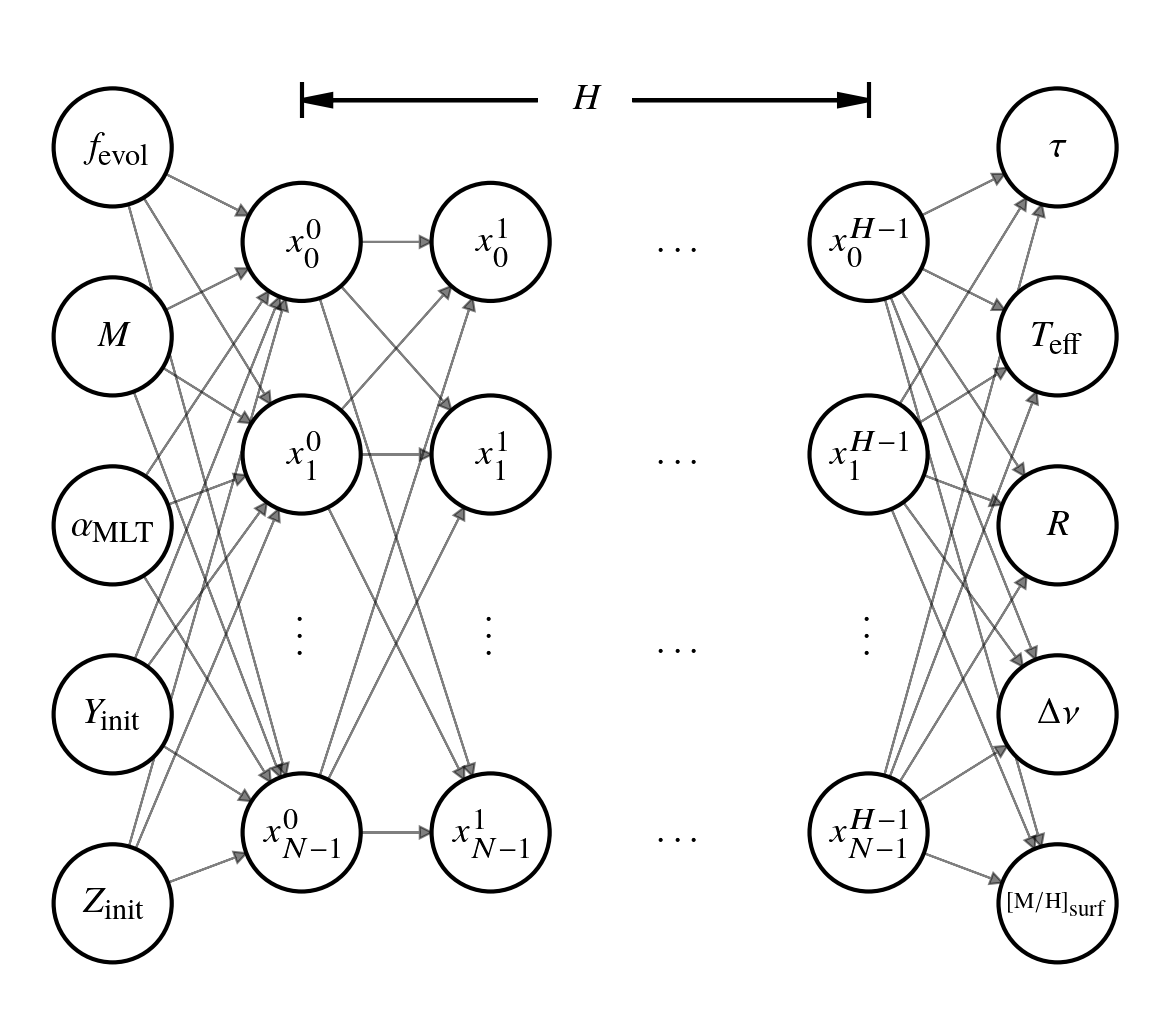
\includegraphics{figures/network_10.png}
    \caption[An artificial neural network comprising $H$ hidden layers with $N$ neurons per layer.]{An artificial neural network comprising $H$ hidden layers with $N$ neurons per layer. Arrows connecting the nodes represent tunable weights.}
    \label{fig:net}
\end{figure}

In this work, we considered a fully-connected ANN, where each neuron in layer $j-1$ is connected to every neuron in layer $j$. The output of the $k$-th neuron in layer $j$ is, 
%
\begin{equation}
    x_{j, k}=f_j(\boldsymbol{w}_{j, k} \cdot \boldsymbol{x}_{j-1} + b_{j, k}),
\end{equation}
%
where $f_j$ is the \emph{activation} function for the $j$-th layer, $\boldsymbol{w}_{j, k}$ are the weights connecting all the neurons in layer $j-1$ to the current neuron, and $b_{j, k}$ is the bias. This generalises such that the output of the $j$-th layer is,
%
\begin{equation}
    \boldsymbol{x}_{j}=f_j(\boldsymbol{W}_{j} \cdot \boldsymbol{x}_{j-1} + \boldsymbol{b}_{j}),
\end{equation}
%
where $\boldsymbol{W}_j$ is the matrix of weights leading to all neurons in the $j$-th layer. For a regression ANN, we typically have a linear activation function applied to the final output layer. Layers of neurons between the input and output layers are called \emph{hidden} layers. Therefore, the output of a network of $H$ hidden layers with initial input $\boldsymbol{\mathbb{X}}$ is,
%
\begin{equation}
    \widetilde{\boldsymbol{\mathbb{Y}}} = \boldsymbol{W}_{H} \cdot f_{H-1}(\dots f_1(\boldsymbol{W}_1 \cdot f_0(\boldsymbol{W}_{0} \cdot \boldsymbol{\mathbb{X}} + \boldsymbol{b}_{0}) + \boldsymbol{b}_1) ) + \boldsymbol{b}_{H}.
\end{equation}
%
We also restricted our configuration to an ANN with the same number of neurons, $N$ in each hidden layer. Hereafter, we refer to our choice of neurons per layer, $N$ and hidden layers, $H$ as the \emph{architecture} (see Fig. \ref{fig:net}).

To fit the ANN, we used a set of training data, $\boldsymbol{\mathbb{D}}_\mathrm{train} = \{\boldsymbol{\mathbb{X}}_i, \boldsymbol{\mathbb{Y}}_i\}_{i=1}^{N_\mathrm{train}}$ comprising $N_\mathrm{train}$ input-output pairs. We split the training data into pseudo-random batches, $\boldsymbol{\mathbb{D}}_\mathrm{batch}$ because this has been shown to improve ANN stability and computational efficiency \citep{Masters.Luschi2018}. The set of predictions made for each batch is evaluated using a \emph{loss} function which primarily comprises an error function, $E(\boldsymbol{\mathbb{D}}_\mathrm{batch})$ to quantify the difference between the training data outputs ($\boldsymbol{\mathbb{Y}}$) and predictions ($\widetilde{\boldsymbol{\mathbb{Y}}}$). We also considered an additional term to the loss called \emph{regularisation} which helps reduce over-fitting \citep{Goodfellow.Bengio.ea2016}. During fitting, the weights are updated after each batch using an algorithm called the \emph{optimizer}, back-propagating the error with the goal of minimising the loss such that $\widetilde{\boldsymbol{\mathbb{Y}}} \approx \boldsymbol{\mathbb{Y}}$ \citep[see e.g.][]{Rumelhart.Hinton.ea1986}.

We trained the ANN using \textsc{TensorFlow} \citep{Abadi.Barham.ea2016}. We varied the architecture, number of batches, choice of loss function, optimizer, and regularisation during the optimisation phase. For each set of ANN parameters, we initialised the ANN with a random set of weights and biases and minimised the loss over a given number of \emph{epochs}. An epoch is defined as one iteration through the entire training dataset, $\boldsymbol{\mathbb{D}}_\mathrm{train}$. We tracked the loss for each ANN using an independent validation dataset to determine the most effective choice of ANN parameters (see Appendix \ref{sec:opt}).

\subsection{Train, Validation, and Test Data}\label{sec:train}

%%%%%%%%%%%%%%%%%%%%%%%%%%%%%%%%%%%%%%%%%%%%%%%%%%

%%%%%%%%%%%%%%%% TRAIN-TEST SPLIT %%%%%%%%%%%%%%%%

We built the train and validation datasets from the outputs of the grid of stellar models in Section \ref{sec:grid}. This included the input parameters: $M$, $\mlt$, $Y_\mathrm{init}$, and the initial heavy-elements fraction, $Z_\mathrm{init}$. We also included the $\teff$, $\log g$, $\dnu$, stellar age ($\tau$), radius ($R$), surface metallicity ($\metallicity_\mathrm{surf}$), and other chemical composition information generated by the models. We determined the fractional MS lifetime, $f_{\mathrm{MS}} = \tau / \tau_{\mathrm{MS}}$, of each evolutionary track by taking $\tau_{\mathrm{MS}}$ as the age when the central hydrogen fraction, $X_c < 0.01$. We then cut data where $f_{\mathrm{MS}} < 0.01$ to remove points on the grid prior to the MS. Once we had refined the data from the grid of models, we randomly sampled \num{7.736e6} points to use as the training dataset, with the remaining $\sim \num{2e6}$ points given to the validation dataset. We varied our choice of ANN input and output parameters among those available in the dataset during tuning (see Appendix \ref{sec:opt}).

Additionally, we produced a test dataset of $\sim \num{2e6}$ stellar models evolved using \textsc{MESA}. Values for the initial $M$, $\metallicity$, $Y$, and $\mlt$ were chosen randomly within the range of grid parameters described in Table \ref{tab:grid} such that they spanned the breadth of the grid in an unbiased manner. We prepared this dataset in the same way as the training set, but also constrained it to $\tau < \SI{15}{\giga\year}$ because we consider ages above $\sim \SI{15}{\giga\year}$ unphysical and such points are sparse in the training data. The test dataset was set aside and evaluated on the final ANN.

\subsection{Tuning}\label{sec:opt}

%%%%%%%%%%%%%%%%%%%%%%%%%%%%%%%%%%%%%%%%%%%%%%%%%%

%%%%%%%%%%%%%%%%%% OPTIMIZATION %%%%%%%%%%%%%%%%%%

We trained an ANN to reproduce stellar observables according to our choice of physics with greater accuracy than typical observational precisions. We experimented with a variety of ANN parameter choices, such as the architecture, activation function, optimisation algorithm, and loss function. We tuned the ANN parameters by varying them in both a grid-based and heuristic approach, each time evaluating the accuracy using the validation dataset.

During initial tuning, we found that having stellar age as an input was unstable, because it varied heavily with the other input parameters. We mitigated this by introducing an input to describe the fraction of time a star had spent in a given evolutionary phase, $f_\mathrm{evol}$. 
%
\begin{equation}
    f_\mathrm{evol} = \begin{cases}
        f_\mathrm{MS},\quad &f_\mathrm{MS} \leq 1\\
        1 + \frac{\tau\,-\,\tau_\mathrm{MS}}{\tau_\mathrm{end}\,-\,\tau_\mathrm{MS}},\quad &f_\mathrm{MS} > 1
    \end{cases}\label{eq:fevol}
\end{equation}
%
where $\tau_\mathrm{end}$ is the age of the star at the end of the track,
%
\begin{equation}
    f_\mathrm{MS} = \frac{\tau}{\tau_\mathrm{MS}},
\end{equation}
%
and $\tau_\mathrm{MS}$ is the MS lifetime. A star with $0.01 < f_\mathrm{evol} \leq 1.0$ is in its MS phase, burning hydrogen in its core, and $1.0 < f_\mathrm{evol} \leq 2.0$ has left the MS. Consequently, $f_\mathrm{evol}$ gives the ANN information about the internal state of the star which affects the output observables. Otherwise, $f_\mathrm{evol}$ has little physical meaning, although it could be interpreted as a measure of the evolutionary phase of the star.

We also observed that the ANN trained poorly in areas with a high rate of change in observables, likely because of poor grid coverage in those areas. To bias training to such areas, we calculated the gradient in $\teff$ and $\log g$ between each point for each stellar evolutionary track and used them as optional weights to the loss during tuning. These weights multiplied the difference between the ANN prediction and the training data in our chosen loss function.

After preliminary tuning, we chose the ANN input and output parameters to be $\boldsymbol{\mathbb{X}} = \{f_\mathrm{evol}, M, \mlt, Y_\mathrm{init}, Z_\mathrm{init}\}$ and $\boldsymbol{\mathbb{Y}} = \{\log(\tau), \teff, R, \dnu, \metallicity_\mathrm{surf}\}$ respectively. A generalised form of our neural network is depicted in Fig. \ref{fig:net}. The inputs corresponded to initial conditions in the stellar modelling code and the outputs corresponded to surface conditions throughout the lifetime of the star, except for age which is mapped from $f_\mathrm{evol}$.

We standardised the training dataset by subtracting the median, $\mu_{1/2}$ and dividing by the standard deviation, $\sigma$ for each input and output parameter. We found that the ANN performed better when the training data was scaled in this way as opposed to no scaling at all. We present the parameters used to standardise the training dataset in Table \ref{tab:std}.

\begin{table}
    \centering
    \caption[The median and standard deviation for each parameter in the training data, used to standardise the dataset.]{The median, $\mu_{1/2}$ and standard deviation, $\sigma$ for each parameter in the training data, used to standardise the dataset.}
    \label{tab:std}
    \begin{tabular}{lcccccccccc}
\toprule
{} & \multicolumn{5}{c}{Input} & \multicolumn{5}{c}{Output} \\
{} & $f_\mathrm{evol}$ & $M\,(\si{\solarmass})$ & $\mlt$ & $Y_\mathrm{init}$ & $Z_\mathrm{init}$ & $\log(\tau/\si{\giga\year})$ & $\teff\,(\si{\kelvin})$ & $R\,(\si{\solarradius})$ & $\dnu\,(\si{\micro\hertz})$ & $\metallicity_\mathrm{surf}\,(\si{\dex})$ \\
\midrule
$\mu_{1/2}$ &             0.865 &                  1.000 &  1.900 &             0.280 &             0.017 &                        0.790 &                5566.772 &                    1.224 &                     100.720 &                                     0.081 \\
$\sigma$    &             0.651 &                  0.118 &  0.338 &             0.028 &             0.011 &                        0.467 &                 601.172 &                    0.503 &                      42.582 &                                     0.361 \\
\bottomrule
\end{tabular}

\end{table}

We found that the optimal choice of architecture ($N$ and $H$) varied depending on our choice of other ANN parameters. Therefore, each time we explored a new parameter, we trained an ANN with a grid of $(N,H)$ ranging from $(32, 2)$ to $(512, 10)$.

We evaluated the performance of three activation functions: the hyperbolic-tangent, the rectified linear unit \citep[ReLU;][]{Hahnloser.Sarpeshkar.ea2000, Glorot.Bordes.ea2011} and the exponential linear unit \citep[ELU;][]{Clevert.Unterthiner.ea2015}. Although the ReLU activation function out-performed the other two in speed and accuracy, the resulting ANN output was not smooth. The discontinuity in the ReLU function, $f(x) = \max(0, x)$ in turn caused the output to be discontinuous. This made the ANN difficult to sample for our choice of statistical model (see Section \ref{sec:hbm}). Out of the remaining activation functions, ELU performed the best, providing a smooth output which was well-suited to our probabilistic sampling methods.

We compared the performance of two optimisers: Adam \citep{Kingma.Ba2014} and stochastic gradient descent \citep[SGD; see e.g.][]{Ruder2016} with and without momentum \citep{Qian1999}. Both optimizers required a choice of \emph{learning rate} which determined the rate at which the weights were adjusted during training. We found that Adam performed well, but the validation loss was noisy as a function of epochs as it struggled to converge. The SGD optimizer was less noisy than Adam, but it was difficult to tune the learning rate. However, SGD with momentum allowed for more adaptive weight updates and out-performed the other configurations.

There are several ways to reduce over-fitting, from minimising the complexity of the architecture, to increasing the size and coverage of the training dataset. One alternative is to introduce weight regularisation. So-called L2 regularisation adds a term, $\sim \lambda_k \sum_i w_{i, k}^2$ to the loss function for a given hidden layer, $k$ which acts to keep the weights small. We varied the magnitude of $\lambda_k$ and found that if it was too large it would dominate the loss function, but if it was too small then performance on the validation dataset was poorer.

We compared the choice of two error functions: mean squared error (MSE) and mean absolute error (MAE). The former is widely used among ANNs because it is more sensitive to large errors. However, we tracked both metrics regardless of which was added to the loss function and found that MAE converged faster. Although MAE is less effective at large errors, we found that these were typically at the edges of the grid and the accuracy was good enough everywhere else.

\begin{figure}[tb]
    \centering
    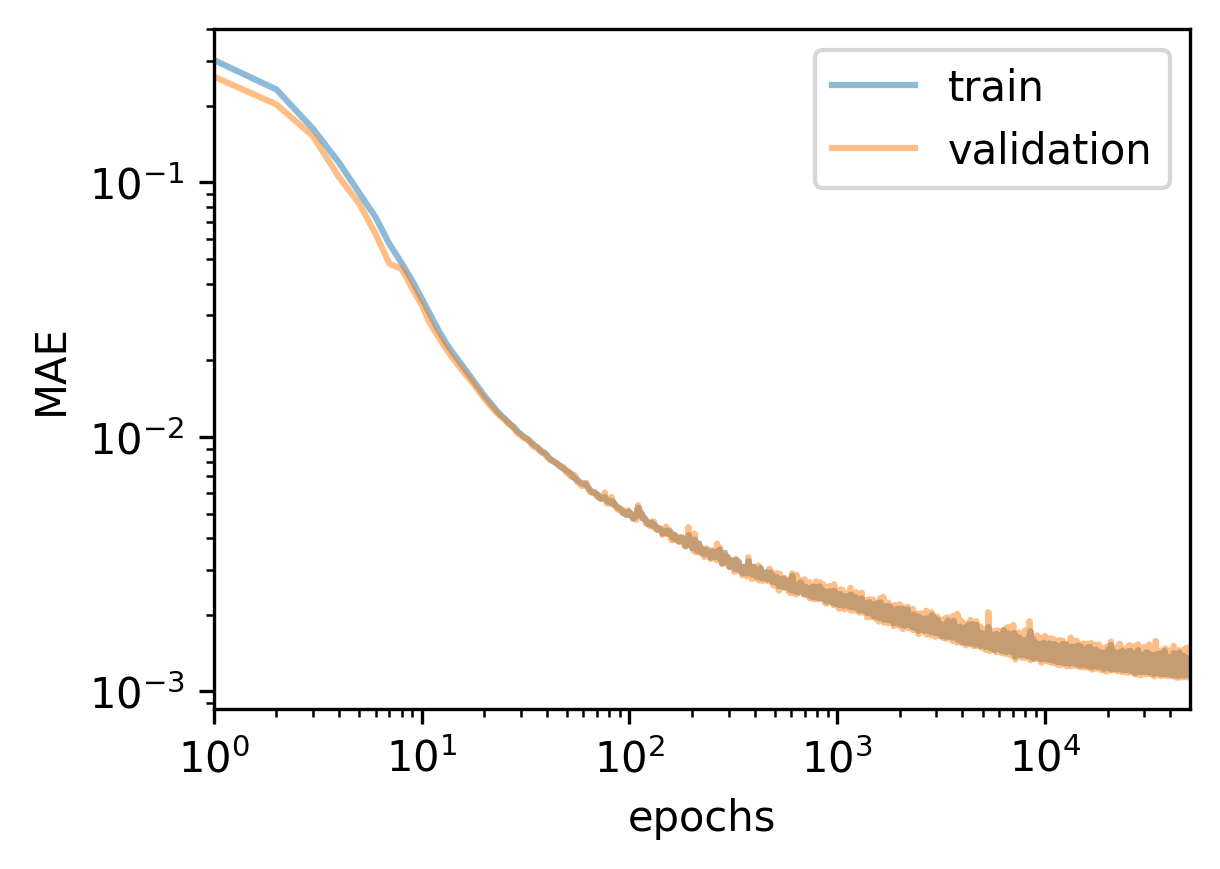
\includegraphics{figures/loss.png}
    \caption{The MAE as a function of epochs for the train and validation datasets.}
    \label{fig:loss}
\end{figure}

After extensive tuning, we opted for an ANN with $N=128$ neurons in each of $H=6$ hidden layers. Each of the hidden layers used an ELU activation function and L2 weight regularisation with $\lambda = \num{1e-6}$. We trained the ANN for \num{50000} epochs with a \num{500} training data batches each containing \num{15472} input-output pairs. To fit the ANN, we used an SGD optimiser with an initial learning rate of \num{1e-4} and momentum of \num{0.999} with an MAE loss function. Training took $\sim \SI{48}{\hour}$ on an NVidia Tesla V100 graphics processing unit (GPU). In Fig. \ref{fig:loss} we show the training and validation MAE as a function of epochs for the final ANN configuration. The training and validation loss were comparable throughout training.

\subsection{Testing}\label{sec:test}

%%%%%%%%%%%%%%%%%%%%%%%%%%%%%%%%%%%%%%%%%%%%%%%%%%

%%%%%%%%%%%%%%%%%%% Validation %%%%%%%%%%%%%%%%%%%

The test dataset contained $\sim \num{2e6}$ stellar models evolved in the same way as the training dataset, but with initial conditions chosen randomly across the range of the grid. We made predictions for the test dataset, deriving luminosity from the output radius and effective temperature, using the final trained ANN as described in Appendix \ref{sec:opt}. We then evaluated the accuracy of the ANN by taking the difference between the test truth and ANN prediction, $x_\mathrm{true} - x_\mathrm{pred}$. 

\begin{figure}[tb]
    \centering
    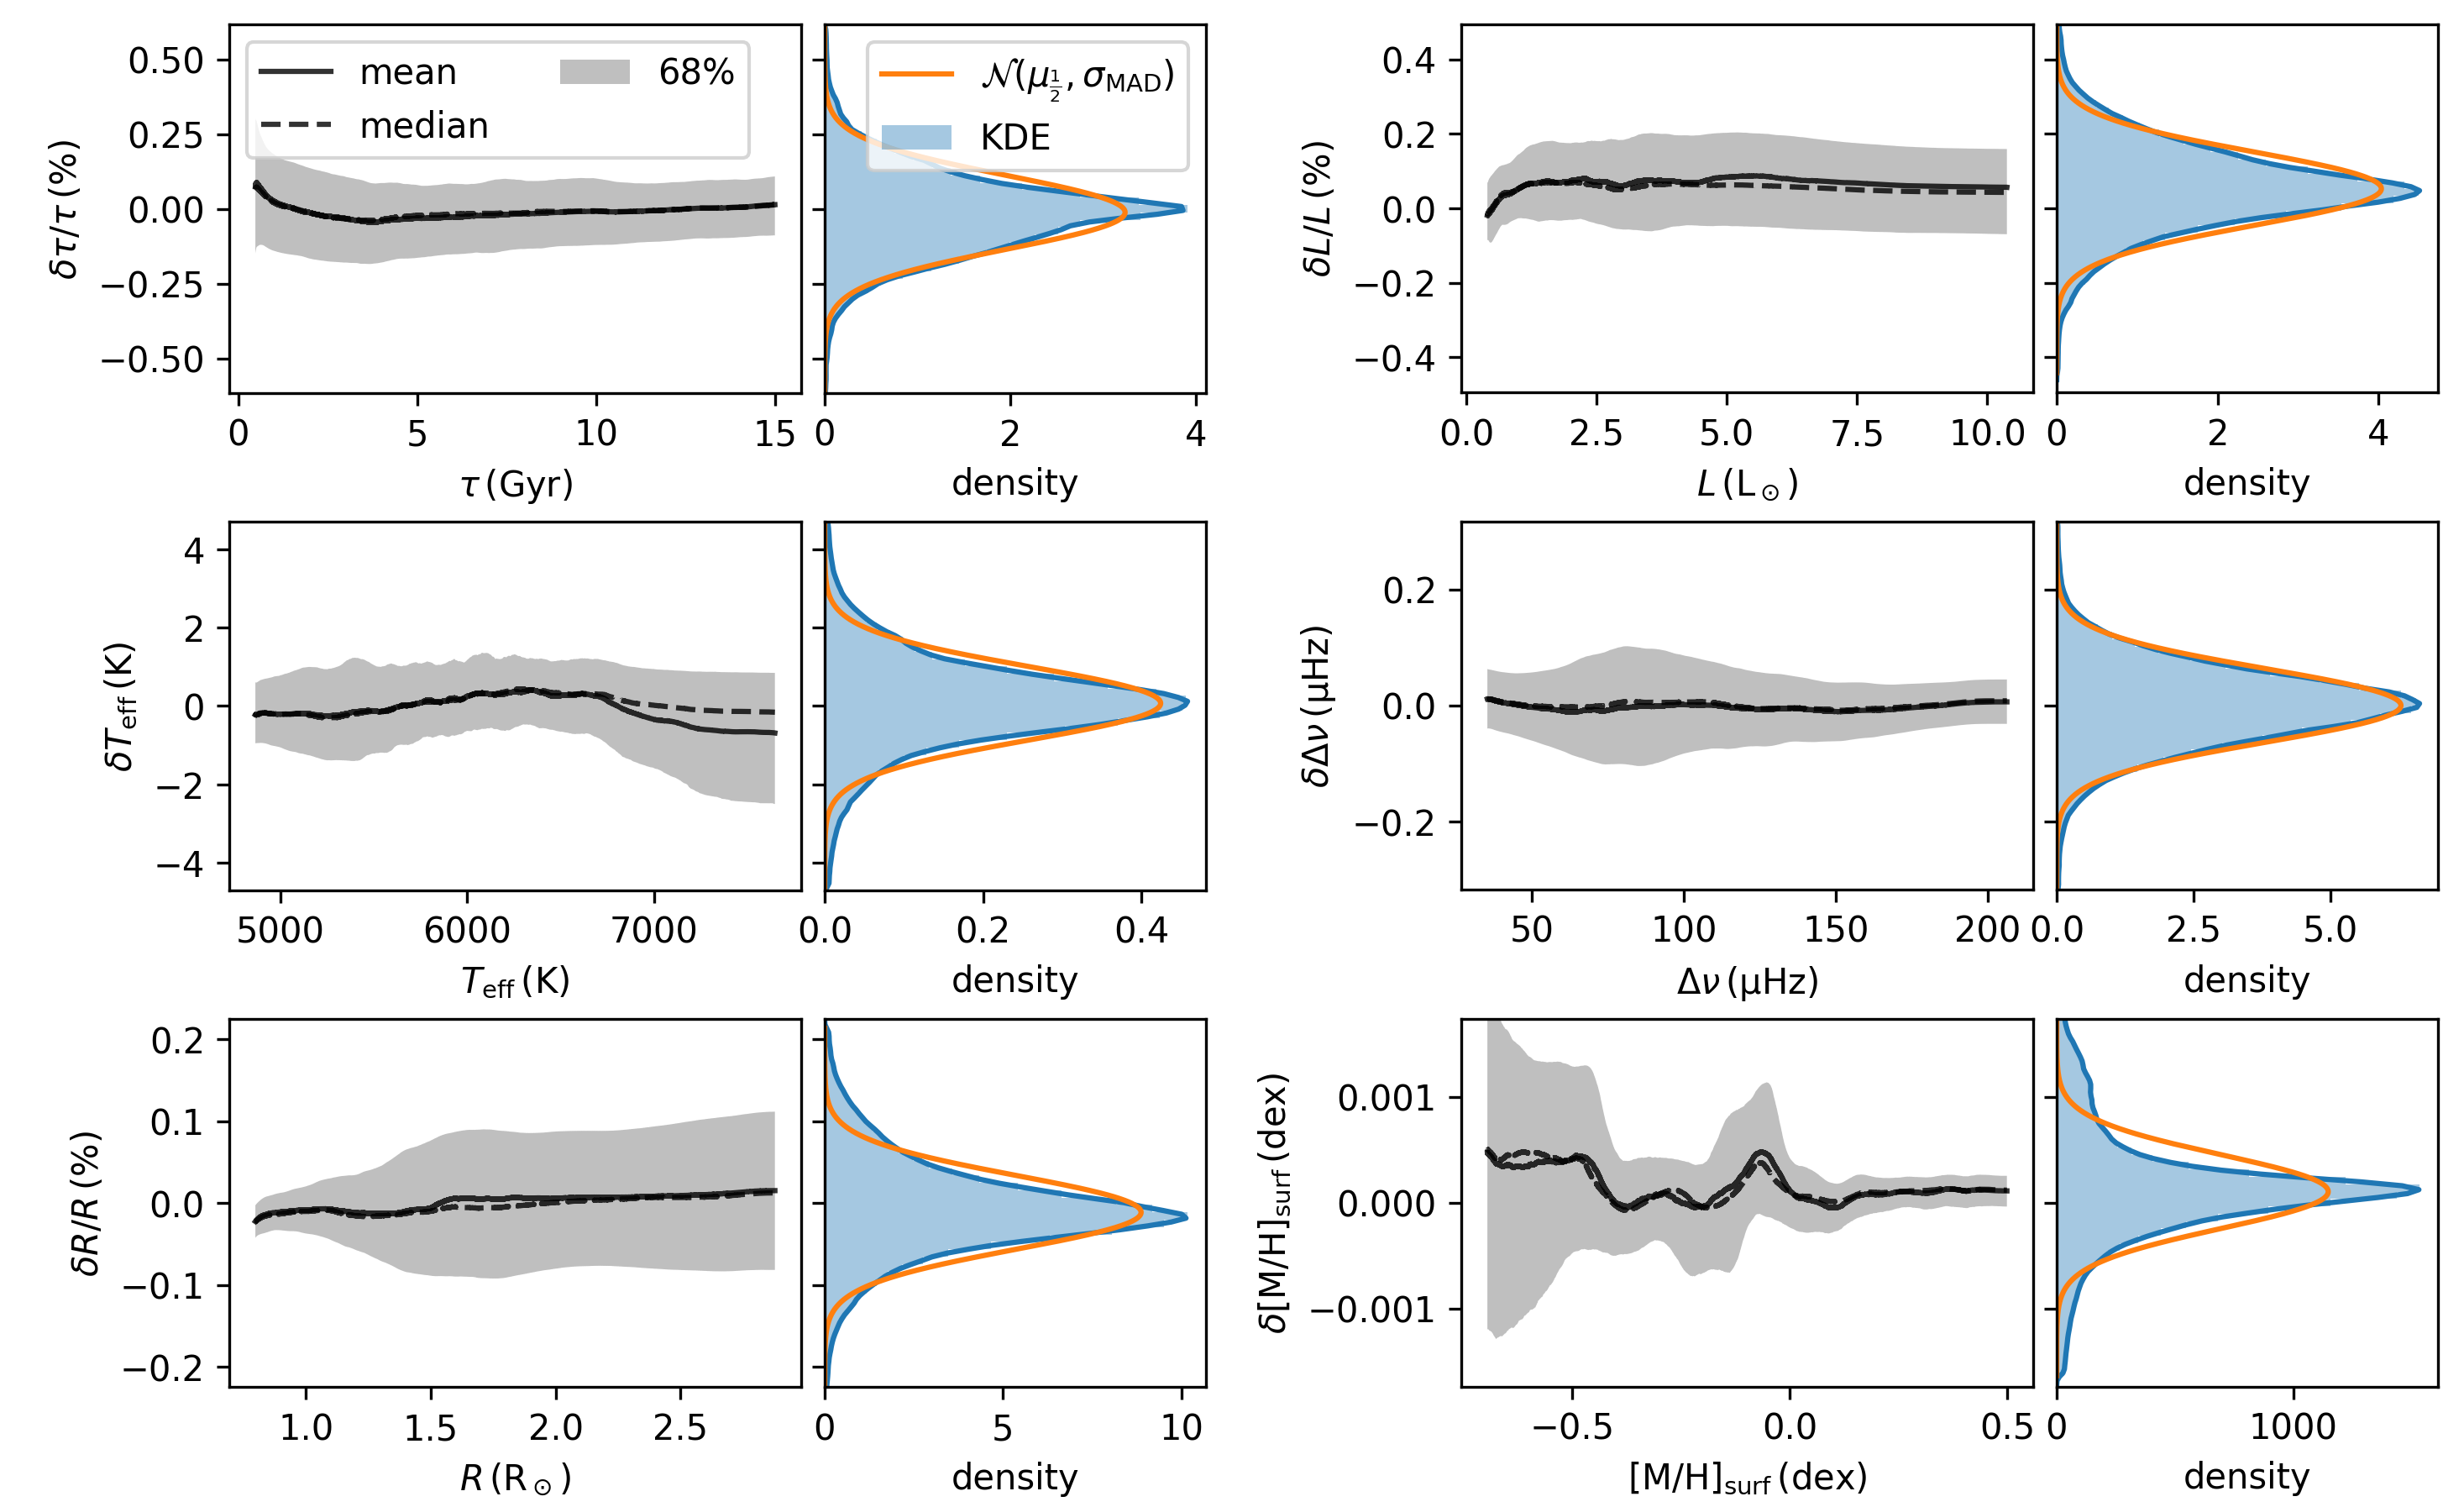
\includegraphics[width=\linewidth]{figures/test_random_wide.png}
    \caption[The error between a given parameter in the test dataset and the ANN prediction for that parameter.]{\emph{Left}: the rolling error between a given parameter in the test dataset ($\mathbb{Y}$) and the ANN prediction for that parameter ($\widetilde{\mathbb{Y}}$) where $\delta \mathbb{Y} = \widetilde{\mathbb{Y}} - \mathbb{Y}$. \emph{Right}: a kernel density estimate (KDE) of the error and a normal distribution centred on the median, $\mu_{1/2}$ with an estimator for the standard deviation from the median absolute deviation, $\sigma_\mathrm{MAD}$.}
    \label{fig:test}
\end{figure}

We found good agreement between the test dataset and ANN predictions, within typical observational uncertainties. We noted that the largest errors lay at the boundaries of the training data and in areas sparsely populated by the grid. This is apparent in Fig. \ref{fig:test} where we plot the test error against each parameter. For example, the spread in error increases for $\metallicity_\mathrm{surf} < -0.5$ where training data is sparse at the edge of the grid. However, the accuracy is very good within the observed range covered by our sample of 81 dwarfs and subgiants. Hence, we chose the median absolute deviation (MAD) as an estimator of the spread in error because it is less sensitive to large errors at the grid boundary than the standard deviation.

\begin{table}
	\centering
	\caption[The median error and median absolute deviation of the error for each ANN output parameter from the test dataset.]{The median error, $\mu_{1/2}$ and median absolute deviation of the error, $\sigma_\mathrm{MAD} = 1.4826\cdot\mathrm{median}(|E(\mathbb{Y}) - \mu_{1/2}|)$ for a given ANN output parameter, $\mathbb{Y}$ from the test dataset. The error, $E(\mathbb{Y})$, is given in the table header, where $\delta \mathbb{Y} = \widetilde{\mathbb{Y}} - \mathbb{Y}$.}
	\label{tab:test}
    \begin{tabular}{lcccccc}
\toprule
Error &  $\delta \tau/\tau\,(\%)$ &  $\delta T_\mathrm{eff}\,(\mathrm{K})$ &  $\delta R/R\,(\%)$ &  $\delta L/L\,(\%)$ &  $\delta \Delta\nu\,(\mathrm{\mu Hz})$ &  $\delta [\mathrm{M}/\mathrm{H}]_\mathrm{surf}\,(\mathrm{dex})$ \\
\midrule
$\mu_{1/2}$           &                    -0.012 &                                  0.070 &              -0.011 &               0.053 &                                0.00022 &                                                         0.00010 \\
$\sigma_\mathrm{MAD}$ &                     0.123 &                                  0.941 &               0.045 &               0.099 &                                0.06341 &                                                         0.00035 \\
\bottomrule
\end{tabular}
    
\end{table}

To represent the accuracy of the ANN, we present the median, $\mu_{1/2}$ and MAD estimator, $\sigma_\mathrm{MAD} = 1.4826\cdot\mathrm{median}(|E(x) - \mu_{1/2}|)$ of the error ($E(x)$) in Table \ref{tab:test}. The median is close to zero for all parameters, showing little systematic bias in the ANN. The MAD is also lower than observational uncertainties quoted in Section \ref{sec:data}. The spread in error for $\dnu$ of $\SI{0.06}{\mu\Hz}$ is comparable to that of observations with the best signal-to-noise. However, the error in $\dnu$ predictions is also comparable to other systematic uncertainties in $\dnu$ discussed in Section \ref{subsec:seismo_model}. Therefore, a robust model which takes account of systematic uncertainties pertaining to $\dnu$, including those from the ANN, will be explored in future work.

\section{Prior Distributions}\label{sec:beta}

\begin{figure}[tb]
    \centering
    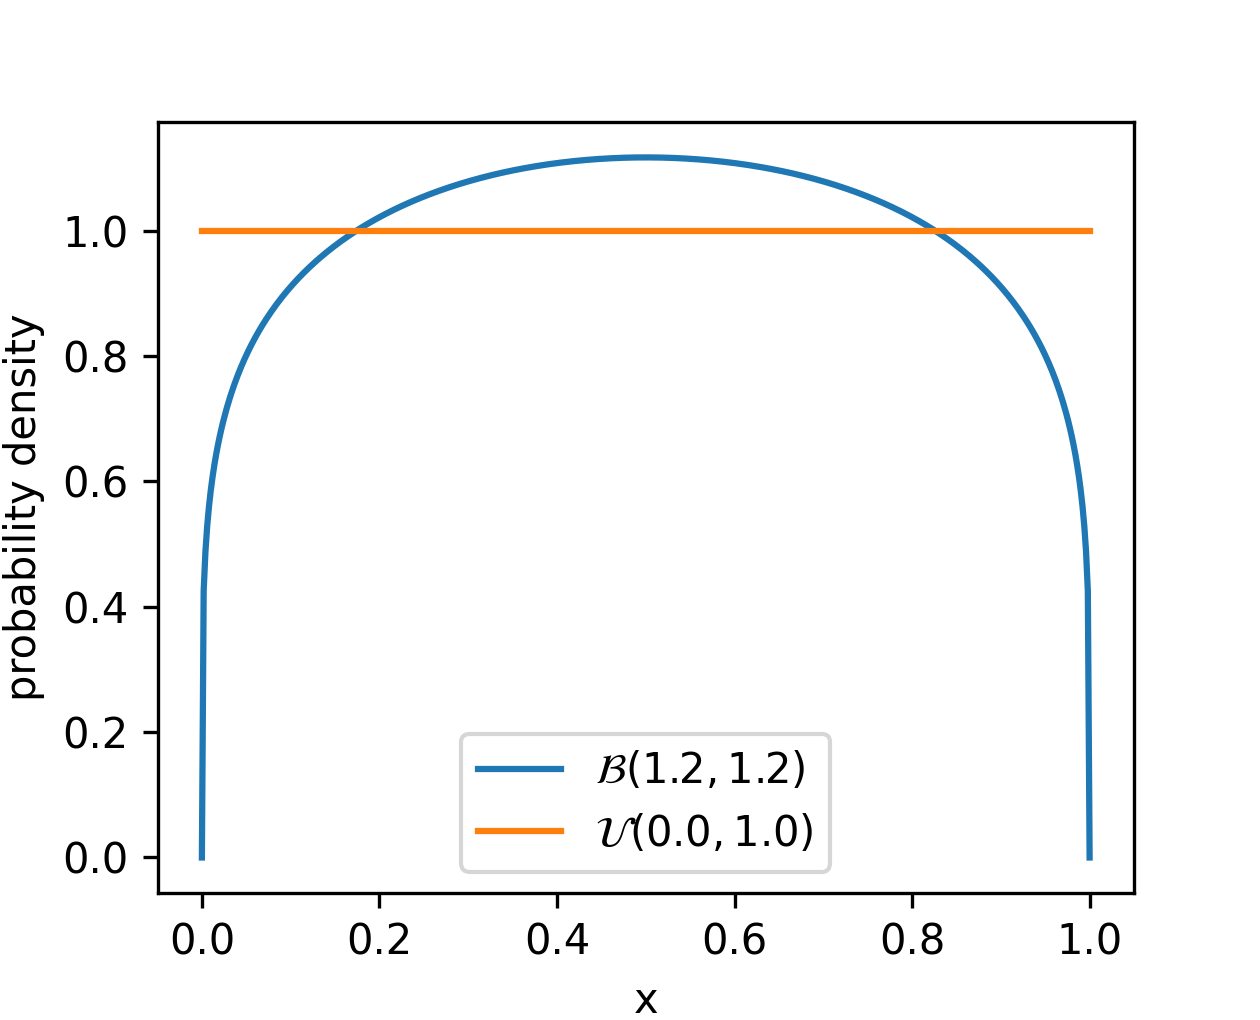
\includegraphics{figures/beta_distribution.png}
    \caption[A beta distribution compared to a uniform distribution.]{A beta distribution ($\mathcal{B}$) with $\alpha = \beta = 1.2$ for some parameter $x$ and a uniform distribution ($\mathcal{U}$) from 0 to 1.}
    \label{fig:beta}
\end{figure}

We chose a transformed beta distribution (see Equation \ref{eq:beta}) as the prior for the non-pooled stellar parameters as an alternative to a uniform distribution. Fig. \ref{fig:beta} shows the beta distribution compared with a uniform distribution for some parameter $x$ from 0 to 1. We found that the continuously differentiable nature of the beta distribution was preferred by the NUTS over the uniform distribution.

\section{The Synthetic Population}\label{sec:test-stars}

%%%%%%%%%%%%%%%%%%%%%%%%%%%%%%%%%%%%%%%%%%%%%%%%%%

%%%%%%%%%%%% THE SYNTHETIC POPULATION %%%%%%%%%%%%

In this section, we present the results for the NP, PP, and MP models run on a synthetic sample of 100 stars with the following initial conditions. We randomly generated initial $M$ and $\metallicity_\mathrm{init}$ uniformly. We drew initial values for $Y_\mathrm{init}$ from a normal distribution centred on the helium enrichment law from Equation \ref{eq:helium} with $\Delta Y / \Delta Z = 1.8$ and $Y_P = 0.247$, and scaled by $\sigma_Y = 0.008$. We also generated initial values for $\mlt$ from a normal distribution centred on $\mu_\alpha = 2.0$ and scaled by $\sigma_\alpha = 0.08$.

We evolved the synthetic stars to randomly chosen ages using \textsc{MESA}. We then took the output $\tau$, $\teff$, $L$, $\dnu$, and $\metallicity_\mathrm{surf}$ from the models and used these as true values for each of the stars. We added random noise to the observed quantities centred on the true values with a standard deviation of 2.2 per cent in $\teff$, 3.5 per cent in $L$, \SI{0.9}{\micro\hertz} in $\dnu$, and \SI{0.07}{\dex} in $\metallicity_\mathrm{surf}$ chosen to be representative of the APOKASC sample.

\subsection{Stellar Parameters}

We found that the NP model recovered the true values for the individual stellar parameters, but the uncertainties were unreliable. The observational quantities alone were not good enough to constrain $Y_\mathrm{init}$ and $\mlt$. As a result, their distributions were truncated at the bounds of their priors. These boundary effects skewed the marginalised posterior means for $Y_\mathrm{init}$ and $\mlt$ towards the centre of the prior (0.28 and 2.0 respectively).

The PP model recovered true values for the synthetic stars with more reliable uncertainty than the NP model. The addition of pooling $Y_\mathrm{init}$ and $\mlt$ between the stars improved their uncertainty which reduced the effects of the prior as seen in the NP model. We found little difference between the results of the PP and MP models.

\begin{figure}[tb]
    \centering
    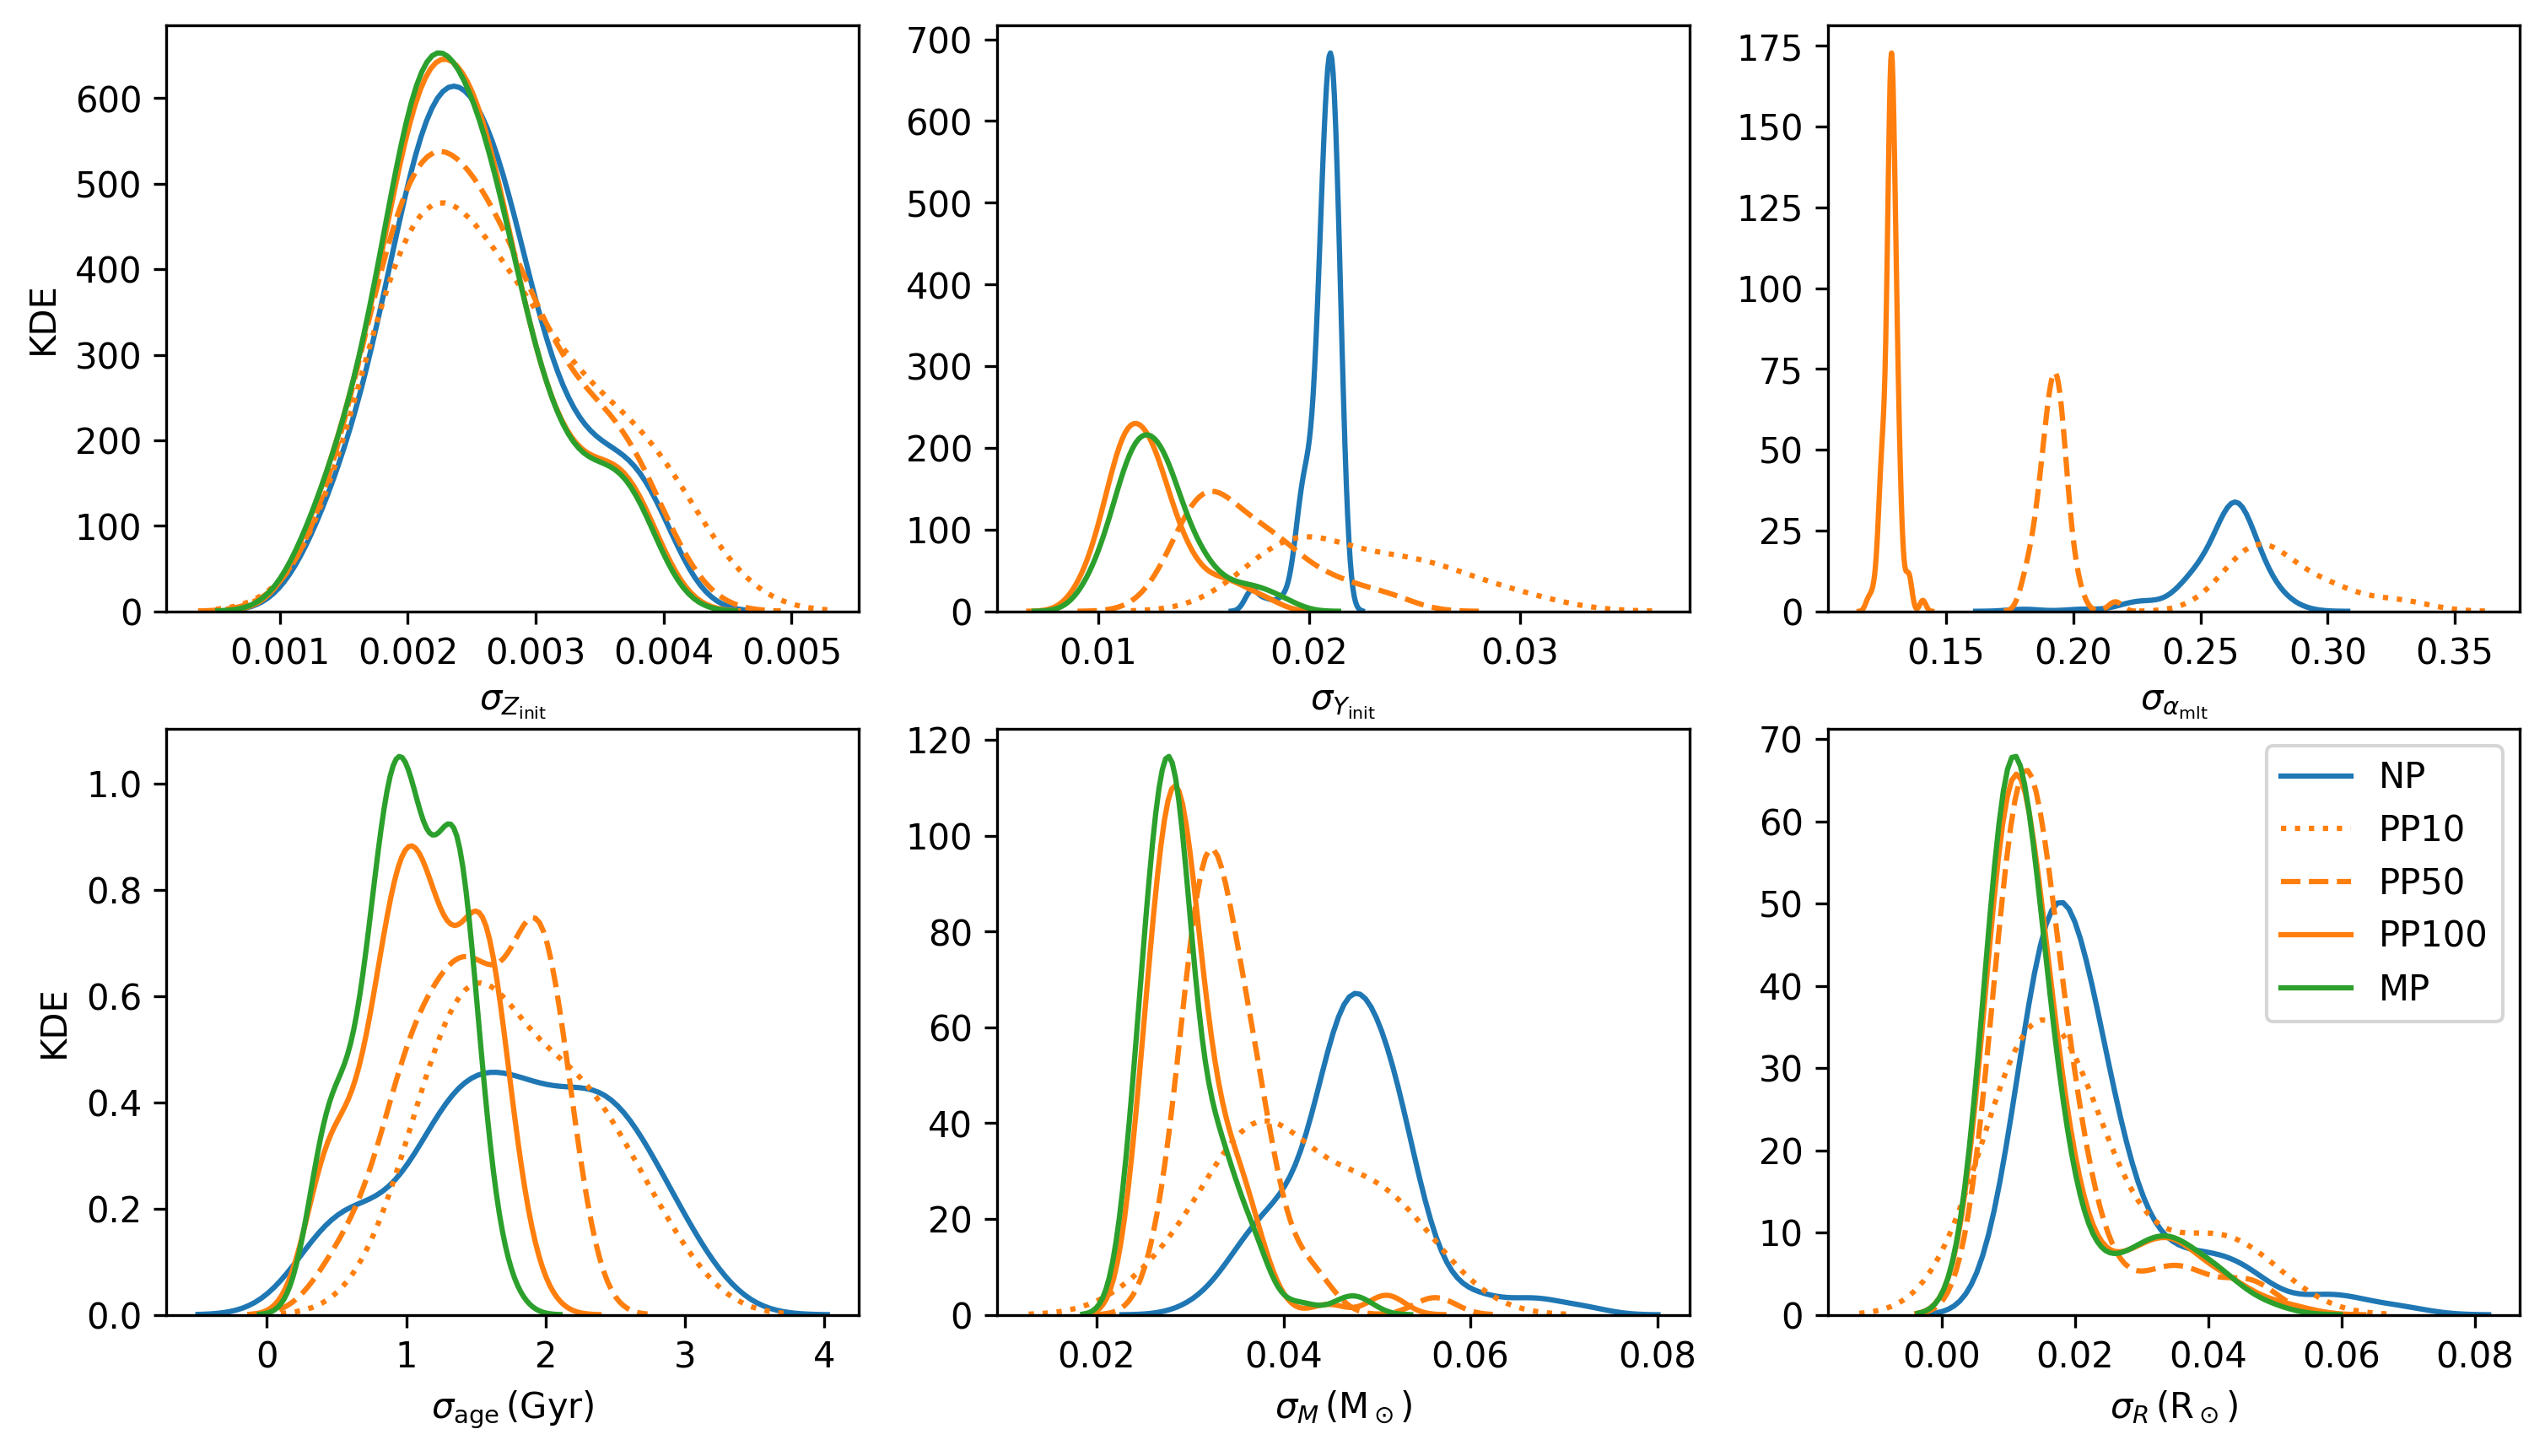
\includegraphics[width=\textwidth]{figures/shrinkage.png}
    \caption[Kernel density estimates of the distributions of statistical uncertainties from each model for the sample of synthetic stars.]{Kernel density estimates (KDEs) of the distributions of statistical uncertainties from each model for the sample of synthetic stars. The PP model was run with 10, 50 and 100 stars and is denoted PP10, PP50, and PP100 respectively. The NP and MP models were both run with the full set of 100 stars.}
    \label{fig:shrinkage}
\end{figure}

We reran the PP model with 10 and 50 stars chosen randomly from the sample of synthetic stars. In Fig. \ref{fig:shrinkage}, we show the uncertainties in the several parameters from the results of each of the models. For the two pooled parameters, $Y_\mathrm{init}$ and $\mlt$, the uncertainty reduction due to pooling is most obvious. We see the PP model repeatedly improves on the uncertainties from the NP model when $N_\mathrm{stars}$ is increased. 

In Fig. \ref{fig:shrinkage} we also see a similar reduction in uncertainty for $\tau$, $M$, and $R$, with all models improve upon the NP model. However, we do not see the same effect in $Z_\mathrm{init}$ for which the uncertainty appears dominated by observations of $\metallicity_\mathrm{surf}$ .

\subsection{Population Parameters}

\begin{figure}
    \centering
    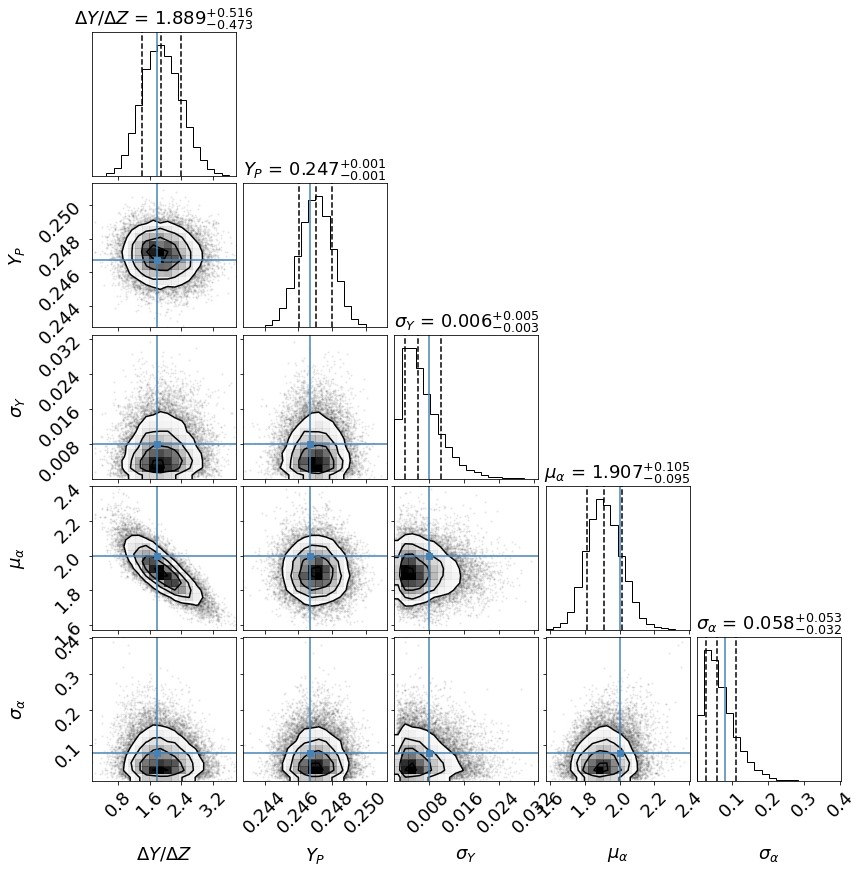
\includegraphics[width=\linewidth]{figures/corner_plot_pp_truths.png}
    \caption[Corner plot showing the marginalised and joint posterior distributions between the PP model hyperparameters for 100 synthetic stars.]{Corner plot showing the marginalised and joint posterior distributions between the PP model hyperparameters for 100 synthetic stars. The true values are shown by the blue lines.}  
    \label{fig:test-corners-pp}   
\end{figure}

In Fig. \ref{fig:test-corners-pp}, we see that the PP model also recovers the hyperparameter truths well, with some noise due to random realisation error. Fitting the model this way has the added benefit over the NP model of improving the inference of the individual stellar parameters, as shown in the previous two sections. We also found that when we ran the PP model with 10 and 50 stars, the uncertainties on the hyperparameters also shrank with increasing $N_\mathrm{stars}$.

\begin{figure}
    \centering
    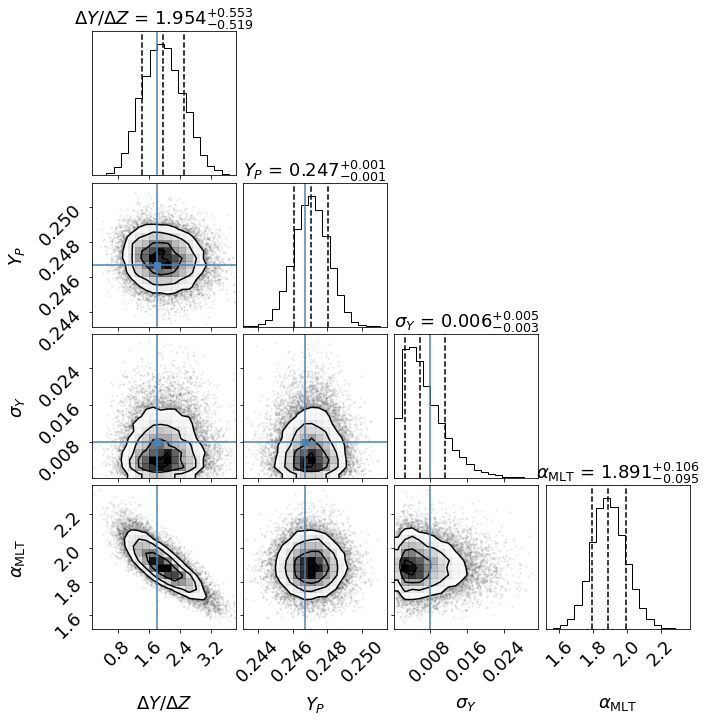
\includegraphics[width=0.82\linewidth]{figures/corner_plot_mp_truths.png}
    \caption{The same as Fig. \ref{fig:test-corners-pp} but for the MP model.}
    \label{fig:test-corners-mp} 
\end{figure}

Fig. \ref{fig:test-corners-mp} shows the hyperparameter results for the MP model. Here, $\mlt$ was assumed to be the same for all stars. This model also recovers the true hyperparameters for helium well, and the assumed value for $\mlt$ is within uncertainty of the true $\mu_\alpha$.

\section{The Sun as a Star}\label{sec:sun-res}

%%%%%%%%%%%%%%%%%%%%%%%%%%%%%%%%%%%%%%%%%%%%%%%%%%

%%%%%%%%%%%%%%% THE SUN AS A STAR %%%%%%%%%%%%%%%%

Our model consistently recovers the Sun when modelled in each of the NP, PP, and MP models. In Table \ref{tab:sun-out} we present the results for the Sun as a star from the NP model to show what we obtain without the influence of any other stars in the sample. We show the marginal and joint posterior distributions for the solar parameters from the NP model in the corner plot in Fig. \ref{fig:sun-results}.

We found some differences between $\mlt$ from our solar model and solar calibrations in the literature produced using \textsc{MESA} with similar input physics. For example, the solar calibration in \citet{Stancliffe.Fossati.ea2016} using \citet{Asplund.Grevesse.ea2009} abundances yields compatible initial abundances, $Z_\mathrm{init} = 0.0149$ and $Y_\mathrm{init} = 0.266$ but $\mlt = 1.783$ which differs from our results by about 10-$\sigma$. This is likely because of a few differences in observed values used for the calibration. \citet{Stancliffe.Fossati.ea2016} used observed helium abundance and convection zone depth measurements from helioseismology. Furthermore, solar calibrations typically include convective envelope overshooting. Presuming overshooting increases mixing in the star, we might expect a lower $\mlt$ to compensate this. Therefore, we stress that the addition of the Sun as a star in our model is with the assumption of our choice of input physics.

\begin{table}
    \centering
    \caption[Solar results from the NP model.]{Solar results from the NP model. The second column shows the median marginalised posterior samples for each parameter with their respective upper and lower 68 per cent credible intervals.}
    \label{tab:sun-out}
    \subcaption*{Input parameters.}
\begin{tabular}{ccccc}
\toprule
                  $f_\mathrm{evol}$ &              $M\,(\si{\solarmass})$ &                           $\mlt$ &                   $Y_\mathrm{init}$ &                      $Z_\mathrm{init}$ \\
\midrule
 $0.517\substack{+0.009 \\ -0.008}$ &  $1.000\substack{+0.001 \\ -0.001}$ &  $2.12\substack{+0.03 \\ -0.03}$ &  $0.262\substack{+0.002 \\ -0.002}$ &  $0.0150\substack{+0.0003 \\ -0.0003}$ \\
\bottomrule
\end{tabular}
\bigskip
\subcaption*{Output parameters.}
\begin{tabular}{ccccc}
    \toprule
                      $\tau\,(\si{\giga\year})$ &      $\teff\,(\si{\kelvin})$ &            $R\,(\si{\solarradius})$ &        $\dnu\,(\si{\micro\hertz})$ & $\metallicity_\mathrm{surf}\,(\si{\dex})$ \\
    \midrule
     $4.6\substack{+0.1 \\ -0.1}$ &  $5777\substack{+12 \\ -12}$ &  $1.001\substack{+0.001 \\ -0.001}$ &  $135.37\substack{+0.14 \\ -0.14}$ &           $0.00\substack{+0.01 \\ -0.01}$ \\
    \bottomrule
    \end{tabular}
\end{table}

\begin{figure}
    \centering
    \includegraphics[width=\textwidth]{figures/corner_plot_sun.png}
    \caption{A corner plot showing the sampled marginal and joint posterior distributions for the Sun as a part of the NP model.}
    \label{fig:sun-results}
\end{figure}

%%%%%%%%%%%%%%%%%%%%%%%%%%%%%%%%%%%%%%%%%%%%%%%%%%


\end{document}
